% Supplementary material, submitted as a separate PDF. Same kit and preamble.

\documentclass[10pt,twocolumn,letterpaper]{article}

\usepackage[review]{cvpr}

%% Packages and macros for the manuscript and the supplementary material.
%% Loaded before hyperref. Based on the CVPR author kit's preamble.tex
%% (original kept in kit/preamble_kit_original.tex).
%% Kept compatible with TeX Live 2018 (the cluster) and Overleaf: no siunitx,
%% no cuted; wide figures use figure*.

\usepackage{multirow}
\usepackage{array}
\usepackage{caption}

%% Inline annotations. Disable before submission (see the README checklist).
\newcommand{\todo}[1]{{\color{red}#1}}
\newcommand{\TODO}[1]{\textbf{\color{red}[TODO: #1]}}
%% Section owner and the registry/protocol IDs behind a paragraph.
\newcommand{\owner}[1]{\textbf{\color{blue}[Owner: #1]}}
\newcommand{\source}[1]{\textbf{\color{teal}[Source: #1]}}
%% \renewcommand{\TODO}[1]{}
%% \renewcommand{\todo}[1]{#1}
%% \renewcommand{\owner}[1]{}
%% \renewcommand{\source}[1]{}

%% Notation used throughout.
\newcommand{\ca}{\mathbf{c}}      % cross-attention seed
\newcommand{\sa}{\mathbf{A}}      % self-attention affinity
\newcommand{\miou}{mIoU}

\DeclareMathOperator*{\argmax}{arg\,max}

\usepackage{longtable}
\usepackage{float}

\definecolor{cvprblue}{rgb}{0.21,0.49,0.74}
\usepackage[pagebackref,breaklinks,colorlinks,allcolors=cvprblue]{hyperref}

\def\paperID{*****}
\def\confName{CVPR}
\def\confYear{2027}

\title{BRACE: Bounded Refinement of Attention from Coarse Envelopes\\for Training-Free Segmentation}
\author{Anonymous CVPR submission}

\begin{document}
\maketitlesupplementary
{\small\setcounter{tocdepth}{2}\tableofcontents}

\section{Method details}
\label{sec:supp_method}
\paragraph{Names in the experiment record.} The registered experiment record (Sec.~\ref{sec:supp_record}) uses internal names: \emph{A3} is the SA-guided layer weighting, \emph{R2} is DenseCRF, \emph{FINE-P2} (also V0, R0) is fine-only propagation with two passes, and \emph{V3} (also R1) is the coarse-to-fine hierarchy with the one-sided cap.

\paragraph{Notation.}
$t$ indexes UNet calls (0--30 for CA, 10--20 for SA), $h$ heads (eight per module) and $m$ modules. $s\in\{16,32,64\}$ is the side of an SA grid, $A^s_{t,h}\in\mathbb R^{s^2\times s^2}$ a row-stochastic SA matrix and $\bar A^s_t$ its head mean. $U$ is bilinear $2\times$ upsampling ($U_{64}$: to $64\times64$), $D$ area downsampling, and $\operatorname{norm}$ min--max normalization. The SA modules are the final transformer block of the decoder at each resolution: \texttt{up\_blocks.1.attentions.2} (16 px), \texttt{up\_blocks.2.attentions.2} (32 px) and \texttt{up\_blocks.3.attentions.2} (64 px). The eleven CA modules are, in sorted \texttt{attn2} order, indices 0, 1 (down, 64 px), 4, 5 (down, 16 px), 6 (mid, 8 px), 7, 8, 9 (up, 16 px) and 13, 14, 15 (up, 64 px). The five 32-pixel modules (2, 3, 10, 11, 12) are excluded.

\paragraph{SA-guided layer weights.}
At each call, $F$ is the conditional query of \texttt{up\_blocks.2.attentions.1}'s CA module, with heads concatenated, and $P_t=\operatorname{softmax}(FF^\top/\sqrt d)$. For CA module $m$, $\tilde S_{t,m}$ is the head-mean SA affinity of the same transformer block, resized to $P_t$'s grid. Following GoCA~\cite{meng2026making}, the key axis is resized bilinearly and the query axis by nearest neighbour. The score $\langle\tilde S_{t,m},P_t\rangle$ is clipped at zero and normalized over $\mathcal M$ within each call (Eq.~2 of the main paper). Figure~\ref{fig:supp_a3} shows the resulting weights. The 8-pixel module receives a quarter of the total weight and the five 16-pixel modules 60\%, while the 64-pixel modules together receive 16\%. The 8-pixel module dominates the first calls, when the image is still coarse.

\begin{figure*}[t]
\centering
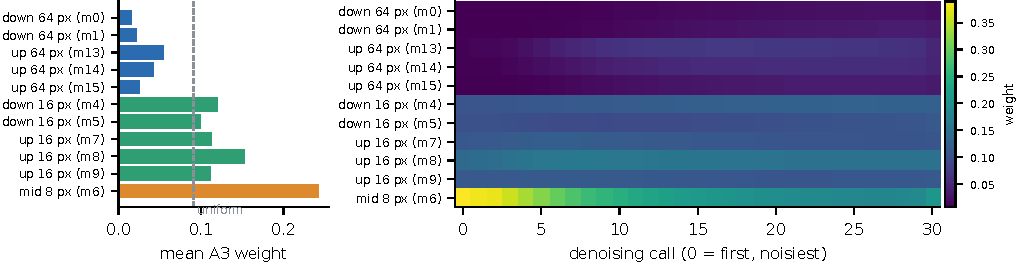
\includegraphics[width=.92\textwidth]{figures/a3_weights.pdf}
\caption{\textbf{SA-guided CA layer weights} (VOC-Sim, all images). Left: mean weight per module, against uniform weighting (dashed). Right: mean weight per denoising call. Weighting by agreement with SA moves 84\% of the weight to the 8- and 16-pixel modules.}
\label{fig:supp_a3}
\end{figure*}

\paragraph{Orientation of the agreement score.}
In our implementation, the resized SA affinity is indexed [key, query], so the score is $\langle\tilde S^\top,P\rangle$ rather than GoCA's $\langle\tilde S,P\rangle$. A paired rerun accumulated both seeds in the same diffusion run (Table~\ref{tab:supp_a3g}). The two seeds agree to Pearson 0.99999 (mean absolute difference 0.0008). The control after DenseCRF changes by $-0.0000$, inside the pre-registered $\pm0.002$ tie band, and the hierarchy's gain is unchanged on the corrected seed. All results use the historical orientation.

\begin{table}[t]
\centering
\footnotesize\setlength{\tabcolsep}{3pt}
\begin{tabular}{@{}lccc@{}}
\toprule
Cell (+ DenseCRF) & VOC forced OOF & folds vs.\ V0 & COCO \\
\midrule
historical SA-guided seed $\rightarrow$ fine only (V0) & .8228 & -- & .6623 \\
GoCA-oriented SA-guided seed $\rightarrow$ fine only (G0) & .8228 & 3/5 & .6617 \\
historical SA-guided seed $\rightarrow$ hierarchy + cap (V3) & .8292 & 5/5 & .6967 \\
GoCA-oriented SA-guided seed $\rightarrow$ hierarchy + cap (G3) & .8304 & 5/5 & .6961 \\
\bottomrule
\end{tabular}
\caption{\textbf{Orientation of the agreement score (paired rerun).} Both seeds come from the same diffusion run. G0 $-$ V0 $=-0.0000$ (CI $[-0.0001,+0.0001]$); G3 $-$ G0 $=+0.0075$ (5/5, CI $[+0.0020,+0.0128]$); G3 $-$ V3 $=+0.0012$ (4/5).}
\label{tab:supp_a3g}
\end{table}


\paragraph{The cap as a projection.}
Let $q\ge0$ be the 32-pixel proposal and $r\ge0$ the 16-pixel parent. Consider the problem
\begin{equation}
\min_{z\ge0}\ \sum_k\Big(z_k\log\frac{z_k}{q_k}-z_k+q_k\Big)\quad\text{s.t.}\quad\sum_{k\in g}z_k\le 4r_g\ \ \forall g .
\end{equation}
The objective and the constraints separate over groups. Within a group, the stationarity condition gives $z_k=q_k e^{-\lambda_g}$ with multiplier $\lambda_g\ge0$. If $\sum_{k\in g}q_k\le4r_g$, then $\lambda_g=0$ and $z=q$; otherwise the constraint is active and $e^{-\lambda_g}=4r_g/\sum_{k\in g}q_k$. This is Eq.~4 of the main paper. Replacing $\le$ by $=$ gives \emph{exact conservation}, $z_k=q_k\,4r_g/\sum_{k\in g}q_k$ for every group. That forces under-budget groups to grow as well, so children must fill a parent's budget even where the parent was wrong. A relaxed variant ($\rho{=}0.5$, Table~\ref{tab:supp_hier}) moves halfway from $q$ towards the conserved solution. The variants with conservation in Table~3 of the main paper operate on per-call distributions (each call normalized to unit mass), whereas the cap operates on the raw maps. This is why the plain hierarchy, rather than the conservation rows, is the cap's direct control: if no group binds, the capped map equals the plain hierarchy exactly.

\paragraph{DenseCRF.}
We call the SimpleCRF wrapper used by OVAM. The unary term is the hard binary mask ($p(\text{fg}){=}1$ inside, $0$ outside), and the parameters are $(w_1,\theta_\alpha,\theta_\beta,w_2,\theta_\gamma,\text{iterations})=(10,80,13,3,3,5)$ on the full-resolution RGB image. Neither these parameters nor the threshold are tuned on COCO-Cap.

\paragraph{Cost.}
All attention is captured during the 30-step generation; nothing is optimized afterwards. The seed reads eleven CA modules at every call, and the hierarchy reads three SA modules at eleven calls. Its largest operation is applying the eight $4096\times4096$ head matrices of the 64-pixel module to one map per call, which is the same operation as fine-only propagation. DenseCRF runs once per image on the CPU.
\clearpage

\section{Building the fine-only baseline}
\label{sec:supp_baseline}
The hierarchy of the main paper replaces the propagation of an earlier, fully registered pipeline: CA seed $\rightarrow$ one 64-pixel SA module, two observation-wise passes $\rightarrow$ DenseCRF, with SA restricted to calls 10--20. This section records how that baseline was selected; it is the ``fine only'' reference throughout the main paper.

\paragraph{One SA module.}
One pass through all sixteen SA modules improves the frozen seed, but the last 64-pixel module (\texttt{up\_blocks.3.attentions.2}) is better. OOF mIoU rises from 0.756 to 0.789 in the combined SA confirmation, all five folds select it, and the paired mean-image gain is $+0.042$ (CI $[+0.037,+0.047]$). Separate screens favoured call 30, resolutions 8+64 and heads $\{1,4,6\}$, but none survived the combination. A Cartesian audit of six CA seeds and twelve SA settings found module 15 the best SA partner for every seed.

\paragraph{Two observation-wise passes.}
For each call--head observation $i$, the fine-only map is
\begin{equation}
p_2=\frac1{|\mathcal I|}\sum_{i\in\mathcal I}A_i^2c .
\end{equation}
The square is taken within each observation before averaging, which is a different operator from $(\frac1{|\mathcal I|}\sum_iA_i)^2c$. A second pass raises OOF mIoU from 0.788 to 0.800, especially for chair ($+0.078$) and person ($+0.030$); a third pass is not promoted. Figure~\ref{fig:supp_depth} shows the trade-off between completion and leakage. In a later diagnostic (A3 seed, calls 10--20, threshold 0.425), pixels first accepted at depth one are 86.5\% true positives on VOC-Sim and 70.8\% on COCO-Cap, but pixels first accepted at depth three are only 39.3\% and 14.0\%.

\begin{figure*}[t]
\centering
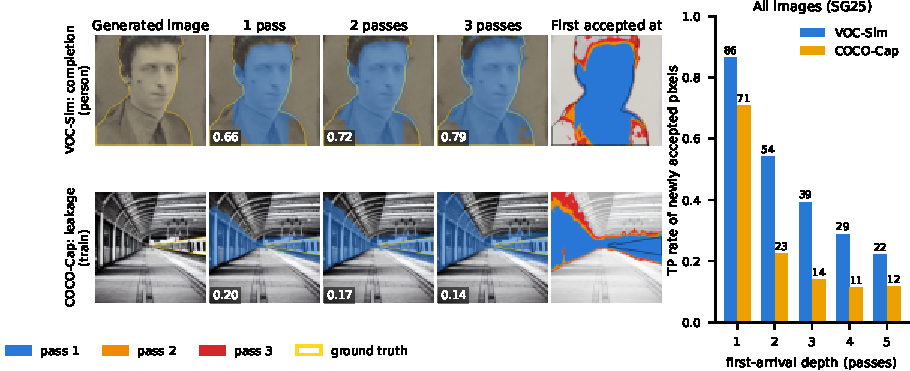
\includegraphics[width=\textwidth]{figures/propagation_depth.pdf}
\caption{\textbf{How far fine SA should propagate.} Left: one, two and three observation-wise passes on a completion example (VOC-Sim, 90th percentile of the two-pass gain) and a leakage example (COCO-Cap, 10th percentile of the three-pass gain), with the pass at which each pixel was first accepted. Right: true-positive rate of newly accepted pixels by depth, pooled over all images. The supplementary gallery (Fig.~\ref{fig:supp_propagation_depth}) applies both rules to both datasets.}
\label{fig:supp_depth}
\end{figure*}

\paragraph{Refinement absorbs propagation gains.}
DenseCRF was selected in all five folds and improved all 20 classes in its screen (0.788$\rightarrow$0.805); with two passes the combined system reached 0.813 OOF. Twenty-four families of graph operators were then registered against one pass (Sec.~\ref{sec:supp_packages}). Observation-reliability operators (consensus edges, sign consensus, robust aggregation, keeping the 50\% most consistent observations) raised one-pass mIoU to 0.797--0.798, which is the level of a second pass. Their per-class gains also correlate with those of the second pass (0.88 and 0.82), and none survived on top of two passes plus DenseCRF. Graph-restricting operators (absorbing walks, confidence locks, reciprocal links, bottlenecks, region labelling) lost. From then on, every candidate was selected on the refined mask.

\paragraph{The SA call window.}
Selecting on the refined mask found one change: SA calls 10--20 instead of 0--30 (Table~\ref{tab:supp_sg22}). Late calls recover some object pixels but also add distant false positives (Fig.~\ref{fig:supp_temporal}), and their utility varies by class.

\begin{table}[t]
\centering
\footnotesize\setlength{\tabcolsep}{3pt}
\begin{tabular}{@{}lccccc@{}}
\toprule
Setting & P2 & R2 & Mid & Forced OOF & COCO \\
\midrule
One pass & -- & -- & -- & .7873 & .6172 \\
Two passes & $\checkmark$ & -- & -- & .7997 & .6246 \\
+ DenseCRF & $\checkmark$ & $\checkmark$ & -- & .8132 & .6372 \\
+ calls 10--20 & $\checkmark$ & $\checkmark$ & $\checkmark$ & .8168 & .6438 \\
\bottomrule
\end{tabular}
\caption{\textbf{The fine-only baseline in one run} (SG22, uniform seed). The registered selector chose MID-P2+R2 in four of five folds (selection path 0.8158 OOF).}
\label{tab:supp_sg22}
\end{table}

\begin{figure*}[t]
\centering
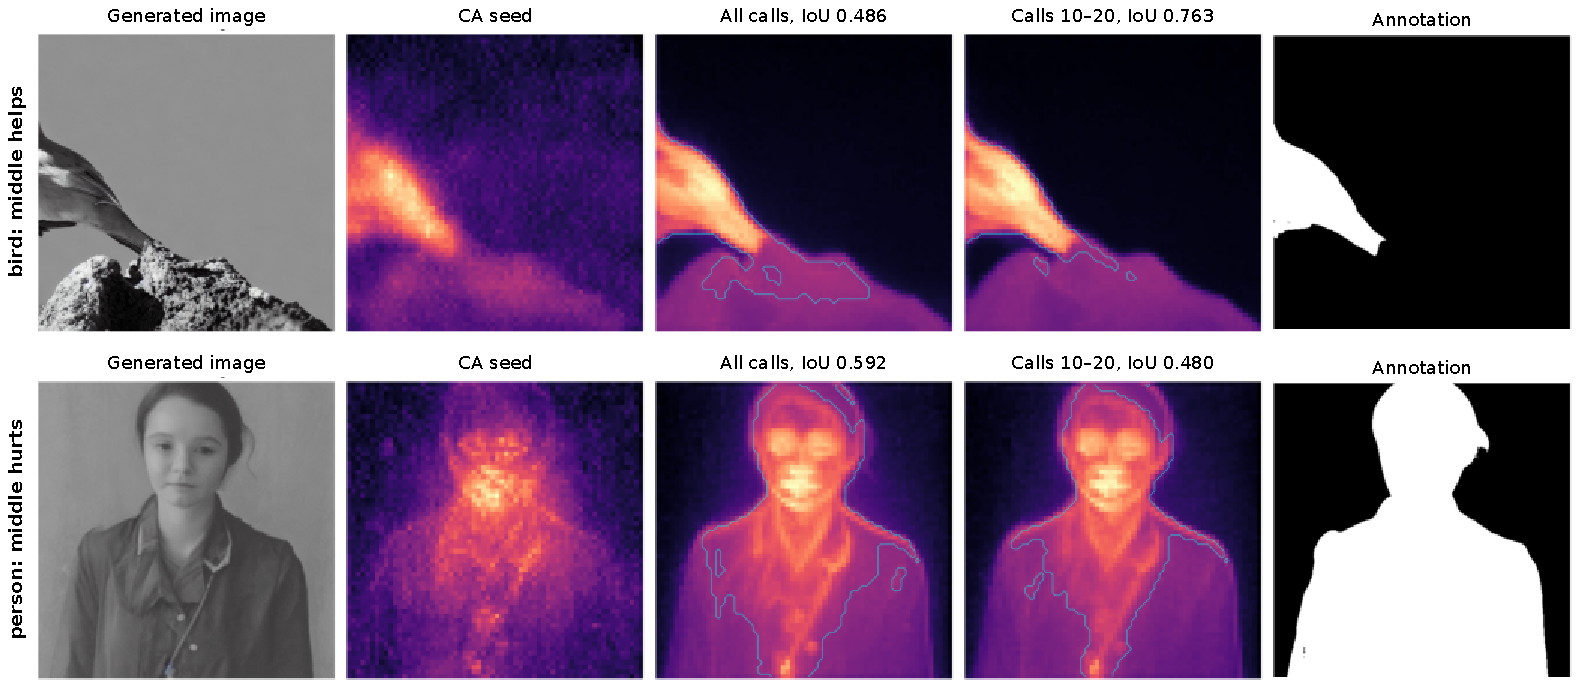
\includegraphics[width=\textwidth]{figures/temporal_tradeoff.pdf}
\caption{\textbf{A temporal window can remove leakage or remove object pixels.} Two VOC-Sim examples from the one-pass, raw-map diagnostic, propagated with SA calls 0--30 or 10--20. Bird gains when a false region is suppressed; person loses when useful extent is suppressed. These are deliberately opposing examples, not images from the final evaluation.}
\label{fig:supp_temporal}
\end{figure*}
\clearpage

\section{Evidence for each stage of the final pipeline}
\label{sec:supp_stages}
Figure~\ref{fig:supp_stages_full} repeats Fig.~2 of the main paper with every intermediate map.

\begin{figure*}[t]
\centering
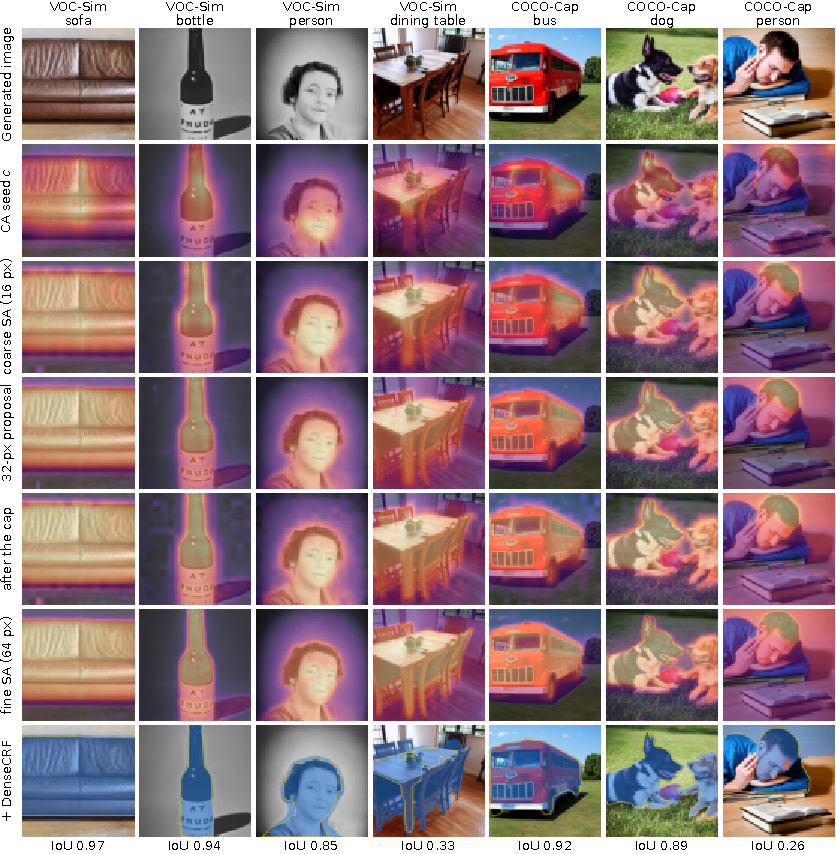
\includegraphics[width=.9\textwidth]{figures/supp_pipeline_c2f.pdf}
\caption{\textbf{Every stage, same fixed-rule images as Fig.~2 of the main paper.} Rows: generated image; A3 seed; coarse 16-pixel SA $r$; 32-pixel proposal $q$; capped map $z$; fine 64-pixel SA $y$; final mask after DenseCRF with the annotation outline. Regenerated maps reproduce the committed per-image scores (largest image-IoU difference 0.005, one COCO-Cap image).}
\label{fig:supp_stages_full}
\end{figure*}

\subsection{Seed}
Figure~\ref{fig:supp_seeds} shows the per-resolution CA maps. 8-pixel CA is blob-like and 16-pixel CA follows object parts, while 64-pixel CA fires on texture and edges throughout the image. A3 down-weights the 64-pixel modules, so its seed is smoother than the uniform one. Table~\ref{tab:supp_sg24} lists every weighting scheme of the same run. Per-pixel content-token rescaling (A1, A4) collapses on COCO-Cap, where the attribution prompt has a single content token, and projected-output head weighting (A2) loses on both benchmarks.

\begin{figure*}[t]
\centering
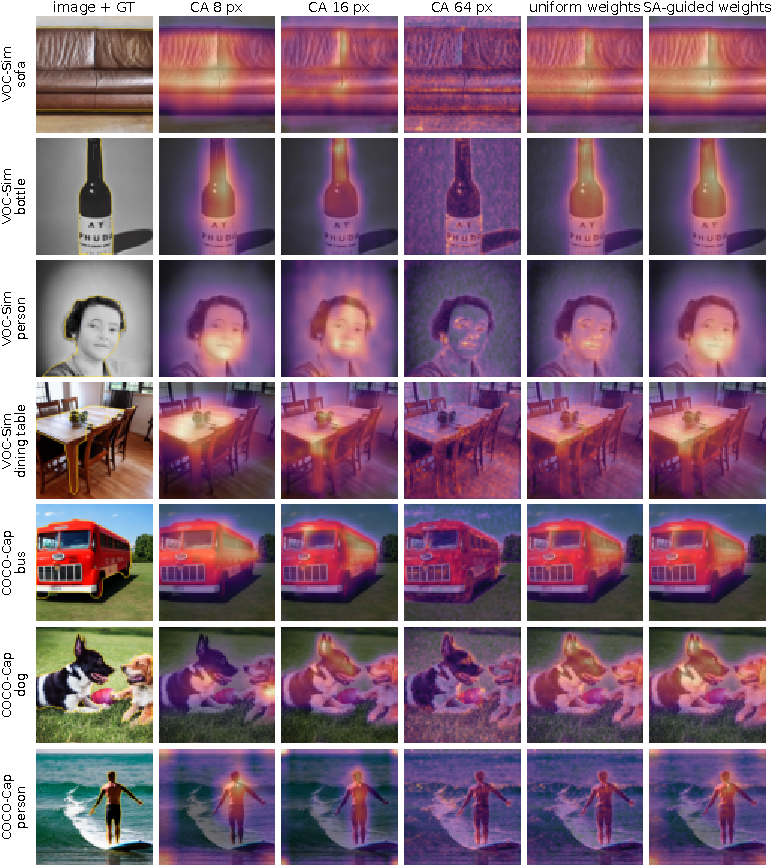
\includegraphics[width=.8\textwidth]{figures/supp_ca_seeds.pdf}
\caption{\textbf{CA by resolution.} Unweighted mean CA of the selected modules at 8, 16 and 64 pixels, the uniform seed and the A3 seed, for the images of Fig.~2 of the main paper.}
\label{fig:supp_seeds}
\end{figure*}

\begin{table}[t]
\centering
\footnotesize\setlength{\tabcolsep}{3pt}
\begin{tabular}{@{}lccc@{}}
\toprule
Weighting & CA only & final (MID-P2+R2) & COCO final \\
\midrule
A0 uniform & .7135 & .8169 & .6437 \\
A1 content-token mass & .6406 & .8005 & .0000 \\
A2 projected head output & .6897 & .8033 & .6366 \\
A3 SA agreement & .7049 & \textbf{.8230} & \textbf{.6620} \\
A4 all three & .6288 & .8004 & .0000 \\
\bottomrule
\end{tabular}
\caption{\textbf{CA weighting schemes} (one run, VOC forced OOF, COCO-Cap frozen). A3 won 4/5 folds against A0 (paired mean-image interval positive). The registered multi-candidate screen chose A3 in only 3/5 folds and kept A0. A3 was adopted afterwards by owner decision.}
\label{tab:supp_sg24}
\end{table}

\subsection{Coarse and fine SA}
Table~\ref{tab:supp_sg25} gives every scale cell of the run behind Fig.~3 of the main paper. Coarse 16-pixel SA alone is far below fine SA on VOC-Sim but competitive on COCO-Cap after R2 (0.665 vs.\ 0.662). Going from 16 to 64 pixels gains on COCO-Cap but not on VOC-Sim, the gap that the cap closes. The reverse order (64$\rightarrow$16) fails, so the order of the scales matters.

\begin{table}[t]
\centering
\footnotesize\setlength{\tabcolsep}{3pt}
\begin{tabular}{@{}lcccc@{}}
\toprule
Propagation (two passes) & VOC & VOC + R2 & COCO & COCO + R2 \\
\midrule
64 px only (fine) & .8097 & .8228 & .6599 & .6621 \\
16 px only (coarse) & .7225 & .7538 & .6282 & .6652 \\
32 px only & .7924 & .8138 & .6693 & .6948 \\
16 $\rightarrow$ 64 & .8020 & .8170 & .6869 & .6975 \\
32 $\rightarrow$ 64 & .8089 & .8217 & .6695 & .6717 \\
64 $\rightarrow$ 16 & .7505 & .7825 & .6403 & .6705 \\
\bottomrule
\end{tabular}
\caption{\textbf{SA scale and order} (one run, A3 seed, calls 10--20; VOC forced OOF, COCO-Cap frozen).}
\label{tab:supp_sg25}
\end{table}

\subsection{The hierarchy: every variant}
Table~\ref{tab:supp_hier} adds the cells omitted from Table~3 of the main paper: budgeted completion (v1 C7--C9), gated completion (v2 V6), and three single changes to the capped hierarchy. The three changes are a cap applied to each head before averaging (W1), a native 16-pixel seed instead of the downsampled one (W2), and a temporal cap of each call by the running mean of earlier calls (W3). None improves on the one-sided cap. The cap binds in 58\% (VOC-Sim) and 65\% (COCO-Cap) of $2\times2$ groups but removes only 7.6\% and 8.3\% of the proposal mass (mean scaling factor of binding groups 0.84).

\begin{table*}[t]
\centering
\footnotesize\setlength{\tabcolsep}{4pt}
\begin{tabular}{@{}llccc@{}}
\toprule
Run & Variant & VOC raw & VOC + R2 & COCO + R2 \\
\midrule
v1 & relaxed conservation, halfway to the projection at both transitions (C5) & .7926 & .8149 & .7059 \\
v1 & exact conservation (both) + background-only completion budget (C7) & .7785 & .8047 & .7054 \\
v1 & exact conservation (both) + semantic/background odds budget (C8) & .7774 & .8031 & .7061 \\
v1 & relaxed conservation + odds budget (C9) & .7951 & .8140 & .7057 \\
v2 & one-sided cap + completion only where $P_1\ge B$ (V6) & .8143 & .8256 & .6792 \\
\midrule
v3 & one-sided cap, reference (R1, = v2 V3) & .8157 & .8293 & .6964 \\
v3 & head-wise cap: $z=\frac18\sum_h\operatorname{cap}(r,A^{32}_hUr)$ (W1) & .8161 & .8294 & .6972 \\
v3 & native 16-px CA seed $c^\ast_{16}$ instead of $D(c)$ (W2) & .8155 & .8281 & .6975 \\
v3 & temporal cap by the mean of earlier calls (W3) & .8116 & .8261 & .6828 \\
\bottomrule
\end{tabular}
\caption{\textbf{Remaining hierarchy variants} (VOC forced OOF, COCO-Cap frozen; each run has its own same-generation references, which agree with Table~3 of the main paper to 0.0003). Against R1 after R2: W1 $+0.0001$ (CI spans 0), W2 $-0.0012$ (2/5), W3 $-0.0032$ (1/5). The head-wise cap removes almost the same mass (7.7\% vs.\ 7.6\%). The native seed correlates 0.996 with $D(c)$. The temporal cap hurts most on small objects ($-0.016$ in the smallest GT-area bin).}
\label{tab:supp_hier}
\end{table*}


\subsection{DenseCRF}
Across the 490 VOC-Sim images, DenseCRF changes the capped pipeline's image IoU by more than 0.005 in 375 images, improving 278. On COCO-Cap it improves 427 of 707 images and 18 of 20 classes (Table~4 of the main paper). Figure~\ref{fig:supp_crf_classes} shows the per-class change.

\begin{figure}[t]
\centering
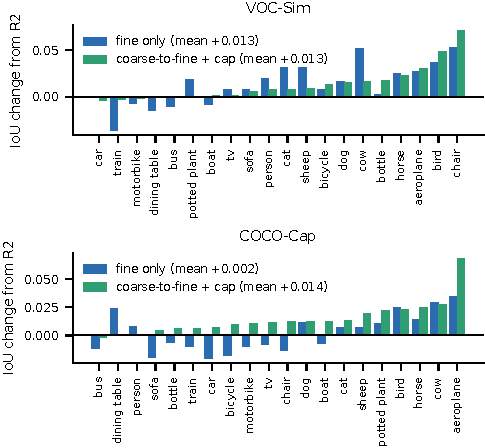
\includegraphics[width=\columnwidth]{figures/supp_crf_classes.pdf}
\caption{\textbf{Per-class effect of DenseCRF} on fine-only and capped coarse-to-fine maps (same run; thresholds from VOC-Sim).}
\label{fig:supp_crf_classes}
\end{figure}
\clearpage

\section{Calibration, thresholds and the sheep failure}
\label{sec:supp_calibration}
\paragraph{Per-image thresholds.}
If the hierarchy's gain is calibration, could a per-image threshold computed from each map recover it, or repair sheep? We tested seven rules on the counts and stored maps of the main run. Each rule's $\tau_I$ is snapped to the 17-point grid, so the existing counts score it exactly, raw and with DenseCRF (the stored maps reproduce the counted mask areas with Pearson $\ge0.9998$). The rules are: T0, the global threshold; T1, Otsu; T2, the crossing of a two-Gaussian fit; T3, $\mu_I+k\sigma_I$; T4, the most stable threshold (smallest area change); T5, the capped map's ranking at the fine-only map's area; and T6, Otsu plus an offset. One-parameter rules choose their parameter inside the training folds. The rule set was registered before the run. Table~\ref{tab:supp_threshold} gives the outcome. No rule improves the capped pipeline. Matching the fine-only map's area (T5) repairs sheep ($-0.007$ instead of $-0.092$) but gives back most of the gain. Otsu helps the fine-only map in four folds but loses 0.021 on COCO-Cap. Two-Gaussian and $\mu{+}k\sigma$ thresholds often fall outside the grid (20--87\% of images).

\begin{table}[t]
\centering
\footnotesize\setlength{\tabcolsep}{2.6pt}
\begin{tabular}{@{}llcccc@{}}
\toprule
Map (+ DenseCRF) & Rule & VOC OOF & vs.\ same map T0 & sheep $\Delta$ & COCO \\
\midrule
fine only & T0 global & .8230 & -- & -- & .6623 \\
fine only & T1 Otsu & .8283 & +.0054 (4/5) & $-$.041 & .6411 \\
fine only & T4 stable & .8255 & +.0026 (2/5) & $-$.042 & .6809 \\
fine only & T6 Otsu$+d$ & .8276 & +.0046 (3/5) & $-$.041 & .6411 \\
\midrule
C2F + cap & T0 global & \textbf{.8293} & -- & $-$.092 & \textbf{.6964} \\
C2F + cap & T1 Otsu & .8238 & $-$.0055 (1/5) & $-$.079 & .6359 \\
C2F + cap & T2 two-Gauss. & .8031 & $-$.0262 (0/5) & $-$.080 & .6258 \\
C2F + cap & T3 $\mu{+}k\sigma$ & .7864 & $-$.0429 (0/5) & $-$.254 & .6498 \\
C2F + cap & T4 stable & .8239 & $-$.0054 (1/5) & $-$.108 & .6722 \\
C2F + cap & T5 fine-only area & .8246 & $-$.0047 (0/5) & $-$.007 & .6659 \\
C2F + cap & T6 Otsu$+d$ & .8297 & +.0004 (2/5) & $-$.090 & .6586 \\
\bottomrule
\end{tabular}
\caption{\textbf{Per-image threshold rules} (after DenseCRF; sheep $\Delta$ vs.\ fine-only T0). Both registered selectors kept the fine-only global threshold. Per-image oracle (best grid threshold per image, using ground truth): 0.896 fine-only vs.\ 0.895 C2F + cap on VOC-Sim.}
\label{tab:supp_threshold}
\end{table}

\paragraph{Sheep.}
The sheep loss is a loss of recall: 294{,}665 fewer true-positive pixels, against only 12{,}173 more false positives. It is concentrated in close-ups where the sheep covers 79--96\% of the frame. Figure~\ref{fig:supp_sheep} shows that the capped map is better on sheep at every threshold above 0.45. Below that, its false positives are twice those of the fine-only map, so sheep cannot use the low threshold it prefers. Across all classes, objects that fill more than 75\% of the frame gain from the cap at every threshold. Sheep is the exception because its surroundings are grouped with it at low thresholds. Figure~\ref{fig:supp_sheep_case} shows the median sheep image.

\begin{figure}[t]
\centering
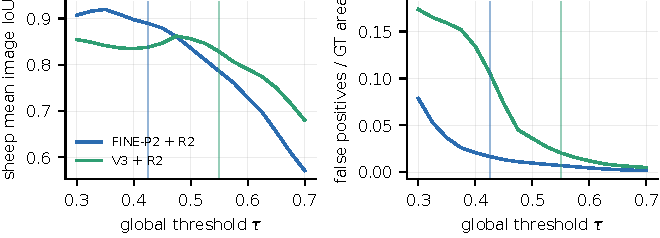
\includegraphics[width=\columnwidth]{figures/supp_sheep_curves.pdf}
\caption{\textbf{Sheep across thresholds} (25 VOC-Sim images, after DenseCRF). Vertical lines: the global thresholds of the two pipelines.}
\label{fig:supp_sheep}
\end{figure}

\begin{figure}[t]
\centering
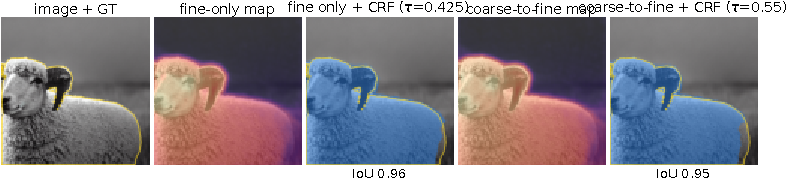
\includegraphics[width=\columnwidth]{figures/supp_sheep_case.pdf}
\caption{\textbf{The median sheep image} (median change of the capped pipeline against fine-only, both after DenseCRF, at their global thresholds).}
\label{fig:supp_sheep_case}
\end{figure}
\clearpage

\section{Selection status of every component}
\label{sec:supp_selection}
Table~\ref{tab:supp_status} lists how each component of the final pipeline entered it. Two components were adopted after the registered rule kept a simpler reference; their registered outcomes are reported here in full.

\begin{table*}[t]
\centering
\footnotesize\setlength{\tabcolsep}{4pt}
\begin{tabular}{@{}>{\raggedright\arraybackslash}p{5.2cm}l>{\raggedright\arraybackslash}p{9.0cm}@{}}
\toprule
Component & How it entered & Registered evidence \\
\midrule
CA without 32-px modules & promoted & 4/5 folds, OOF 0.665$\rightarrow$0.691, paired CI $[+0.015,+0.029]$ \\
All CA heads and calls, conditional query, mean of word pieces & promoted / kept & head and call subsets inside the 0.002 tie band once crossed with scale \\
SA module 15 (64 px) & promoted & 5/5 folds, 0.756$\rightarrow$0.789 \\
Two observation-wise passes & promoted & 0.788$\rightarrow$0.800; confirmed with DenseCRF in 5/5 folds (0.813) \\
DenseCRF, fixed parameters & promoted & 5/5 folds, all 20 classes improved in its screen \\
SA calls 10--20 & promoted & selected after DenseCRF in 4/5 folds (selection path 0.8158 vs.\ 0.8132) \\
SA-guided layer weights & \textbf{owner decision} & forced 4/5 folds, +0.0061 OOF, COCO +0.018; multi-candidate screen chose it in 3/5 folds and kept uniform \\
Coarse-to-fine hierarchy with one-sided cap & \textbf{owner decision} & forced 5/5 folds vs.\ fine-only and plain hierarchy; selectors kept fine-only because the worst class lost 0.057--0.104 in the training folds (guard: 0.050); training-fold gain +0.0039 to +0.0071 \\
\bottomrule
\end{tabular}
\caption{\textbf{Selection status.} ``Owner decision'' marks components adopted after the pre-registered selector retained its reference. Their numbers in the main paper are forced out-of-fold estimates, never in-sample, and their COCO-Cap numbers are frozen transfer.}
\label{tab:supp_status}
\end{table*}

\paragraph{The negative record at a glance.}
Figure~\ref{fig:supp_decision_map} places the 45 registered comparisons of the fine-only phase (studies up to SG28) against the reference of its own run; Sec.~\ref{sec:supp_packages} lists them, and Sec.~\ref{sec:supp_record} gives every cell.

\begin{figure*}[t]
\centering
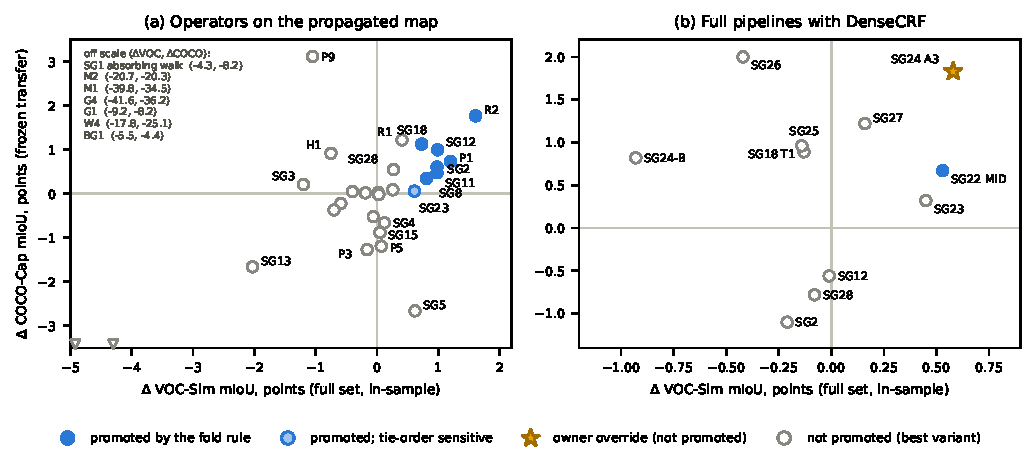
\includegraphics[width=\textwidth]{figures/decision_map.pdf}
\caption{\textbf{The search at a glance.} Each point is one registered experiment family, compared with the reference cell of the same run. $x$: change in VOC-Sim mIoU at each cell's full-VOC threshold (in-sample, descriptive); $y$: change in frozen COCO-Cap transfer. (a) Operators on the propagated map, mostly against one SA pass. The promoted cluster (blue) gains about one point on both datasets, but apart from the second pass and DenseCRF these operators do not improve on two passes plus DenseCRF. (b) Complete pipelines with DenseCRF. Only the middle-call window is promoted, and the SA-guided weighting (star) was adopted by owner decision. Several multi-scale studies raise COCO-Cap transfer but are not selected on VOC-Sim. The map covers the studies up to SG28; later studies, including the hierarchy, are in Secs.~\ref{sec:supp_stages} and \ref{sec:supp_record}.}
\label{fig:supp_decision_map}
\end{figure*}
\clearpage

\section{Protocol}
\label{sec:supp_protocol}
The full protocol, with every registration, result and review in the order they happened, is \texttt{docs/\allowbreak{}ATTENTION\_\allowbreak{}SEGMENTATION\_\allowbreak{}EXPERIMENT\_\allowbreak{}PROTOCOL.md} (130 sections); the registry of experiment families is \texttt{docs/\allowbreak{}ATTENTION\_\allowbreak{}FUSION\_\allowbreak{}AND\_\allowbreak{}TOKEN\_\allowbreak{}IDEAS.md}. This section summarizes the rules that every reported number obeys.

\paragraph{Fixed conditions.}
Stable Diffusion 1.5 generates every image from its released prompt and seed, with 30 scheduler steps, classifier-free guidance 7.5, a float32 model and float16 storage of compact attention. ``Calls 0--30'' are the 31 recorded UNet call indices, inclusive. CA uses the conditional branch for query and key, a softmax over all 77 positions of the padded attribution prompt, and the mean over every tokenizer piece of the class name within each head. All maps are combined on a $64\times64$ grid. Generated images and attention tensors are discarded after scoring; per-image TP, FP and FN at every threshold of the grid are kept, so that folds, bootstrap intervals and later analyses need no regeneration.

\paragraph{Folds.}
\texttt{configs/\allowbreak{}voc\_\allowbreak{}sim\_\allowbreak{}folds.csv} assigns the 490 VOC-Sim images to five class-stratified folds (about five images per class per fold), with a fixed seed, committed before any run. In each outer fold, the method parameter and the mask threshold are chosen on the other four folds and scored on the held-out fold; the reference is treated the same way.

\paragraph{Decision rule (v1.2).}
A candidate is promoted if it improves training-fold mIoU by at least 0.010, or by 0.005--0.0099 with at least 12 of 20 classes improved and no class losing more than 0.05; it must win at least four of five fold votes and give a positive pooled OOF gain. Within 0.002, the simpler setting wins (the reference, then fewer added operations, then fewer free parameters). Each family is screened against its own reference; family winners then go to a combined confirmation.

\paragraph{Registry rules.}
R1: only VOC-Sim selects; COCO-Cap is scored once per frozen pipeline. R2: the frozen CA/SA pair is the reference input. R3: folds and thresholds as above, on the 17-point grid 0.30--0.70. R4--R5: the decision and tie rules above. R6: per-image records, commit and environment for every shard. R7: each package runs in one environment and compares only with its own reference. R8: grids are committed before the run; later changes are logged and labelled post hoc. R9: every package reports fold choices, OOF scores, paired bootstrap intervals, per-class changes and the number of configurations searched. R10: training-free, few-shot and external-segmenter tracks are reported separately. R11: no token is trained on an image of the fold it is scored on.

\paragraph{Deviations.}
Four departures from these rules affect reported numbers, and each is labelled where it appears. (i) The A3 CA weighting was retained by owner decision after the registered selector kept its reference (SG24-A); all later studies (SG25--SG33 and the SG-combined studies) build on it; SG-A3G, which tests the GoCA orientation, is still running. (ii) SG13's candidate cells use a 0--1 threshold grid by 0.005, registered before the run; its controls keep the 17-point grid. (iii) SG22--SG24 shards ran on a mix of V100 and A100 nodes, against R7 (Sec.~\ref{sec:supp_reproducibility}). (iv) SG23's raw promotion depends on the order of tied candidates, which the registration did not fix (Sec.~\ref{sec:supp_reproducibility}).

\section{Every controlled package}
\label{sec:supp_packages}
\owner{each package owner}
\TODO{One subsection per package (CA A/B, CA-C, SA A/B, SA-C, joint audit,
phase 3): fold choices, OOF table, calibration, AP, per-class changes, and the
number of configurations searched. Full per-configuration CSVs are in the
evidence package.}
\source{evidence package A1--A6}

\section{Negative and null results}
\label{sec:supp_negative}
\owner{Claude (artifact audit)}
\TODO{$\sa^\top\ca$; CA-H, SA-T, SA-R and SA-H failing in combination; the
closest joint-audit alternative; the 65{,}535-subset searches as exploratory
maxima.}

\section{Exploratory record}
\label{sec:supp_exploratory}
\owner{Claude (artifact audit)}
\TODO{Tier-B experiments (B1--B17) with the label that their settings were
chosen on the reported images.}
\source{evidence package ledger}

\section{Reproducibility}
\label{sec:supp_reproducibility}
\owner{Claude (artifact audit)}
\TODO{Model, scheduler, seeds and prompts; fold file; environments of every
package; result-package commits; the map from every table and figure to its
source file (paper/README.md).}

\section{Qualitative figures of the fine-only baseline}
\label{sec:supp_gallery}
These figures show the earlier fine-only pipeline of Sec.~\ref{sec:supp_baseline} (uniform seed, two passes through 64-pixel SA, DenseCRF at 0.45). Figure~\ref{fig:supp_gallery} shows, by a fixed rule, the four classes with the lowest class IoU of that pipeline on each dataset, each shown by its median-IoU image. No image was inspected before the choice. The COCO-Cap columns show three different failures. For the chair, propagation leaks into the wooden wall behind it. For the dining table, which fills the frame, the mask covers the plate and bread on it but not its surface. For the bottle, the mask covers both bottles, but only one is annotated, so part of the error is in the label rather than the mask.

\begin{figure*}[t]
\centering
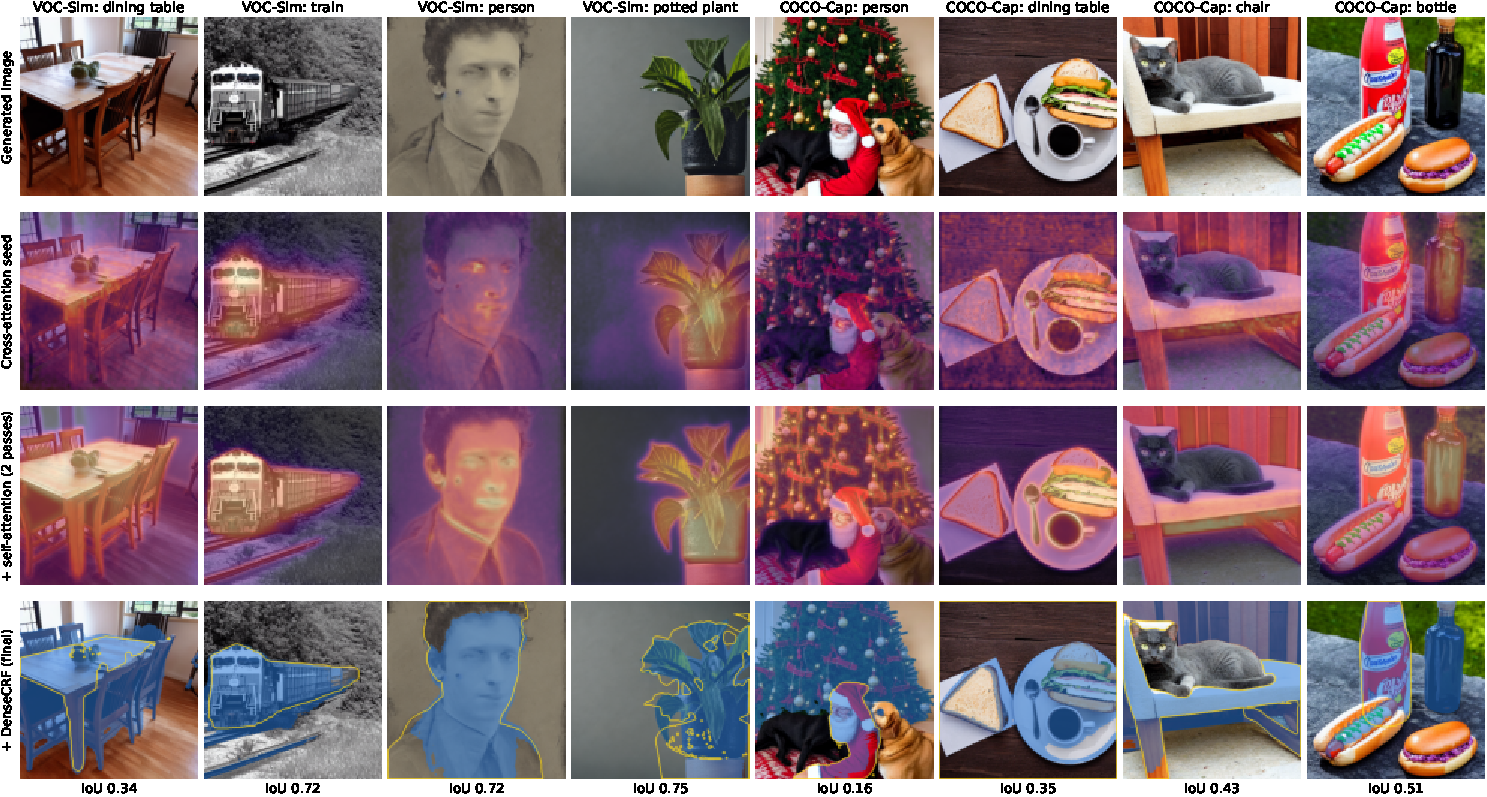
\includegraphics[width=\textwidth]{figures/supp_gallery.pdf}
\caption{\textbf{The weakest classes, one median image each.} Rows: generated image; CA seed; two SA passes; final mask after DenseCRF at 0.45 (blue) with the ground-truth outline (yellow) and the image IoU. Columns: the four lowest class IoUs on VOC-Sim, then on COCO-Cap, from the lowest.}
\label{fig:supp_gallery}
\end{figure*}

\paragraph{CA resolution.} Figure~\ref{fig:supp_ca_example} illustrates the CA resolution decision (Table~2 of the main paper) on one image.

\begin{figure*}[t]
\centering
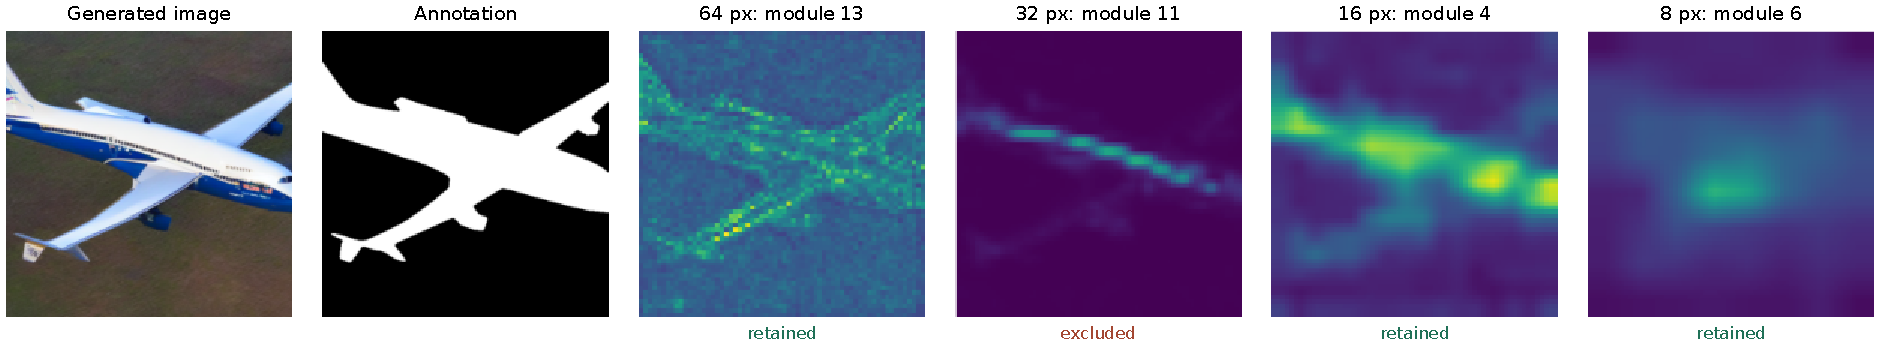
\includegraphics[width=\textwidth]{figures/ca_airplane.pdf}
\caption{\textbf{Why CA resolution is a real design choice.} One VOC-Sim airplane generated image and annotation (left), followed by representative head-averaged CA modules from the same image and all calls. All heatmaps use one color scale. The selected seed retains 8, 16 and 64-pixel modules and omits the 32-pixel group. This visual example motivates the controlled resolution test; the fold-level evidence is in Table~2 of the main paper.}
\label{fig:supp_ca_example}
\end{figure*}

\paragraph{Propagation depth.} Figure~\ref{fig:supp_propagation_depth} applies both selection rules of Fig.~\ref{fig:supp_depth} to both datasets.

\begin{figure*}[t]
\centering
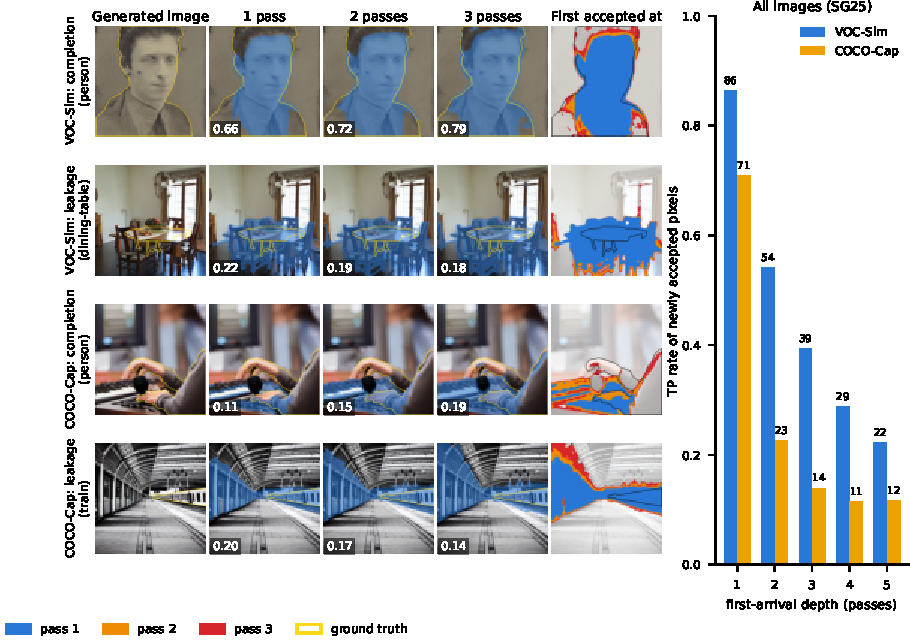
\includegraphics[width=\textwidth]{figures/supp_propagation_depth.pdf}
\caption{\textbf{One, two and three SA passes, both rules on both datasets.} Rows: on each dataset, the image at the 90th percentile of the two-pass gain (completion) and at the 10th percentile of the three-pass gain (leakage), from the all-call raw maps of SG22 at threshold 0.45. Columns and right panel as in Fig.~\ref{fig:supp_depth}.}
\label{fig:supp_propagation_depth}
\end{figure*}

% Complete experiment record. One-column pages; tables come from scripts/paper/supp_experiment_record.py
% (record/*) and from scripts/narmyn/attention/build_evidence.py (evidence/*, copied unchanged).
\onecolumn
\section{Complete experiment record}
\label{sec:supp_record}
This section lists every experiment of the study, including those the paper mentions only in passing. Nothing here is new evidence: every number is read from a committed result file. Three kinds of number appear, and they should not be mixed.
\begin{itemize}
\item \textbf{Out-of-fold (OOF)} VOC-Sim mIoU: a choice made on four folds and scored on the fifth, pooled over the five rotations. This is the number every decision uses.
\item \textbf{Full-VOC} mIoU: a cell at its best threshold on all 490 images. It is in-sample and only describes the cell.
\item \textbf{COCO-Cap} mIoU: frozen transfer at the threshold chosen on VOC-Sim. Nothing is ever chosen on COCO-Cap.
\end{itemize}
Experiments come in three groups: exploratory runs before the fold protocol (B1--B17, Sec.~\ref{sec:supp_record_exploratory}); the controlled screens of the first three phases (A1--A12, P3-C, T-C, Sec.~\ref{sec:supp_record_early}); and the later registered packages (SG1--SG28 and the training-free backlog, Sec.~\ref{sec:supp_record_cells}). Table~\ref{tab:record_ledger} lists all of them; Table~\ref{tab:record_screens} lists every registered fold decision.

\subsection{Ledger and registered decisions}
% Generated by scripts/paper/supp_experiment_record.py; do not edit.
{\scriptsize\setlength{\tabcolsep}{3pt}
\begin{longtable}{@{}l>{\raggedright\arraybackslash}p{5.0cm}>{\raggedright\arraybackslash}p{3.3cm}r>{\raggedright\arraybackslash}p{5.4cm}@{}}
\caption{\textbf{Ledger of every experiment.} B: exploratory, before the fold protocol (in-sample, never used as evidence). A, P3-C, T-C: controlled screens of the first three phases. SG, BL: later registered packages. Sec.: protocol section with the result. Best/decision: for B rows, the best in-sample configuration and mIoU; for controlled rows, the promoted cell(s) or ``none''.}\label{tab:record_ledger}\\
\toprule
ID & Experiment & Status & Cells & Best / decision \\
\midrule
\endfirsthead
\toprule
ID & Experiment & Status & Cells & Best / decision \\
\midrule
\endhead
B1 & CA time windows and resolutions & exploratory, in-sample & 11 & first look at time and resolution \\
B2 & Single and leave-out CA layers & exploratory, in-sample & 24 & layer screening \\
B3 & Joint time x resolution & exploratory, in-sample & 21 & interaction check \\
B4 & Exhaustive CA layer subsets & exploratory, in-sample & 17 & chose BEST\_12 = layers {0, 2, 5, 6, 7, 9, 10, 11, 12, 13, 14, 15} \\
B5 & Threshold x normalization & exploratory, in-sample & 153 & chose percentile 1-99 and threshold 0.45 \\
B6 & Stage-1 suite (heads, time-layer, fusion, cleanup) & exploratory, in-sample & 590 & chose the fixed top-4 CA heads per layer \\
B7 & Self-attention screens and progressive SA & exploratory, in-sample & 5320 & first evidence that SA propagation helps \\
B8 & Full streaming ablations & exploratory, in-sample (choices from B1-B7 frozen) & 6261 & SA at U3.2 (64x64), 4 passes: 0.7777 \\
B9 & Focused SA follow-up & exploratory, in-sample & 1632 & top-4-head seed, 2 passes, t=0.45: 0.7922 \\
B10 & Joint SA head x time x passes x threshold & exploratory, in-sample & 4680 & final method: 4 passes, heads {0,1,2,4,5,6}, calls 15-30, t=0.45, 1\% cleanup: 0.7997 \\
B11 & Component ablation of the final method & exploratory (COCO untuned) & 18 & SA propagation is the largest component \\
B12 & COCO-Cap generalization of the final method & untuned transfer & 6 & 0.5719 $\rightarrow$ 0.6080 \\
B13 & Revised system (1 pass, all 16 CA layers) and its ablation & exploratory; informed by COCO-Cap & 14 & revised system: VOC 0.7824, COCO 0.6322 \\
B14 & CA call windows with all SA heads & exploratory & 4 & no gain over all calls \\
B15 & Clean CA-only screens (pre-sync) & exploratory, in-sample; audited, superseded by A1 & 1573 & ratified as correct; re-run with folds as A1 \\
B16 & OVAM released masks & reference (authors' masks) & 3 & 0.7036 / 0.8247 / 0.6616 \\
B17 & OVAM optimized token and DenseCRF on the final method & exploratory; nothing selected & 32 & token + DenseCRF: VOC 0.8525, COCO 0.6612 \\
A1 & Controlled CA package B: CA-L, CA-H, CA-A & controlled, 5-fold cross-validated & 65961 & CA-L drop modules 10-11; CA-H drop head 1; CA-A keep reference (combined in A3) \\
A2 & Controlled CA package A: CA-T, CA-R (Codex) & controlled, 5-fold cross-validated & 1279 & CA-T keep all calls; CA-R keep 8+16+64 (drop 32x32) (combined in A3) \\
A3 & Controlled CA confirmation (CA-C) and the frozen CA & controlled, 5-fold cross-validated & 6 & frozen CA: CA-R alone (drop the 32x32 modules), all heads \\
A4 & Controlled SA package B: SA-L, SA-H, operator check & controlled, 5-fold cross-validated & 65951 & SA-L only module 15 (U3.2, 64x64); SA-H heads {1, 4, 6}; A x kept (combined in A6) \\
A5 & Controlled SA package A: SA-T, SA-R (Codex) & controlled, 5-fold cross-validated & 1279 & SA-T call 30 only; SA-R resolutions 8+64; both calibration-dependent (combined in A6) \\
A6 & Controlled SA confirmation (SA-C, Codex) and the frozen SA & controlled, 5-fold cross-validated & 13 & frozen SA: module 15 (U3.2) only, all calls, all heads \\
A7 & Joint CA x SA interaction audit (Codex) & controlled, 5-fold cross-validated & 78 & sequential pair kept 5/5; Section 11 unchanged \\
A8 & Phase 3 propagation package (Codex): P1, W3, P2, P6 & controlled, 5-fold cross-validated; threshold chosen in the folds & 40 & two passes mean\_i(A\_i² c) promoted to P3-C \\
A9 & Phase 3 fusion and calibration package: P4, F3, F4, N2-N4, R2 & controlled, 5-fold cross-validated; threshold chosen in the folds & 12 & DenseCRF promoted to P3-C; the rest kept at REF \\
A10 & Released baselines scored with OVAM's procedures & reproduction of published values & 19 & every printed OVAM-notebook value reproduced \\
AN1 & Why a second SA pass helps (analysis, nothing selected) & analysis of committed counts & — & second pass fills under-covered objects; the token seed already covers them; COCO-Cap leakage cancels the gain \\
A11 & Token track B1/B1b: OVAM's optimized tokens on the frozen pipeline & controlled, 5-fold cross-validated; few-shot track (2-3 annotated images per class) & 27 & token promoted on every pipeline: REF 0.787 $\rightarrow$ 0.851 (conditional query) \\
A12 & Token learning B2a/S4/B2b (Codex): retrained tokens, shots, fold-safe token & controlled, fixed T-C pipeline and threshold 0.475; linear-objective variant of OVAM's recipe (audit) & 9 & retrained all-support token = released on VOC-Sim (0.868 vs 0.865), +0.0075 on COCO-Cap; second support gives the gain; released token kept \\
P3-C & P3-C (Sec.~51) & controlled, 5-fold & 30 & promoted: \texttt{P1/\allowbreak{}obs\_\allowbreak{}n2$|$N0/\allowbreak{}global$|$R2/\allowbreak{}crf}, \texttt{P1/\allowbreak{}obs\_\allowbreak{}n2$|$N4/\allowbreak{}otsu$|$R2/\allowbreak{}crf} \\
SG5 & SG5 contrastive cross-attention seed (Sec.~66, 70) & controlled, 5-fold & 40 & promoted: none \\
SG1/SG3 & SG1/SG3 anchored graph refinement (Sec.~68, 71) & controlled, 5-fold & 76 & promoted: none \\
SG3-T & Locked token-SG3 confirmation (Sec.~72, 78, 80) & controlled, 5-fold & 6 & promoted: none \\
SG8 & SG8 observation-consensus propagation (Sec.~73, 78, 80) & controlled, 5-fold & 32 & promoted: \texttt{T/\allowbreak{}A/\allowbreak{}median}, \texttt{W/\allowbreak{}C/\allowbreak{}rho0p80} \\
SG9 & SG9 reciprocal SA propagation (Sec.~74, 78, 80) & controlled, 5-fold & 8 & promoted: none \\
SG10 & SG10 seed-connected bottleneck propagation (Sec.~75, 77, 79) & controlled, 5-fold & 54 & promoted: none \\
SG2 & SG2 consensus-edge SA graph (Sec.~81, 85) & controlled, 5-fold & 56 & promoted: \texttt{T/\allowbreak{}G\_\allowbreak{}cv\_\allowbreak{}g20\_\allowbreak{}n1}, \texttt{W/\allowbreak{}G\_\allowbreak{}cv\_\allowbreak{}g20\_\allowbreak{}n1} \\
SG4 & SG4 SA regions labelled by CA (Sec.~81, 85) & controlled, 5-fold & 40 & promoted: none \\
BL & Training-free Track-A backlog (14 families) (Sec.~82, 83, 86) & controlled, 5-fold & 44 & promoted: none \\
SG11/SG12 & SG11 robust consensus and SG12 reliable observations (Sec.~84, 89) & controlled, 5-fold & 14 & promoted: \texttt{W/\allowbreak{}SG11/\allowbreak{}trim20/\allowbreak{}rho0p80}, \texttt{W/\allowbreak{}SG12/\allowbreak{}top50} \\
SG2+R2 & Locked SG2 + DenseCRF confirmation (Sec.~87, 89) & controlled, 5-fold & 6 & promoted: none \\
SG13 & SG13 target-conditioned region labelling (Sec.~88, 90) & controlled, 5-fold & 7 & promoted: none \\
SG12+R2 & Locked SG12 + DenseCRF confirmation (Sec.~91, 92) & controlled, 5-fold & 5 & promoted: none \\
SG14 & SG14 SG11 x SG12 complementarity (Sec.~91, 92) & controlled, 5-fold & 4 & promoted: \texttt{W/\allowbreak{}SG11/\allowbreak{}trim20/\allowbreak{}rho0p80}, \texttt{W/\allowbreak{}SG14} \\
SG15 & SG15 prior-driven SPEC32 region refinement (Sec.~91, 92, 93) & controlled, 5-fold & 16 & promoted: none \\
SG17 & SG17 reliability-filtered second-pass additions (Sec.~94, 95) & controlled, 5-fold & 4 & promoted: none \\
SG18 & SG18 temporal-windowed one-pass propagation (Sec.~96, 97) & controlled, 5-fold & 5 & promoted: \texttt{W/\allowbreak{}T1} \\
SG18-T1+R2 & SG18 follow-up: T1 window + DenseCRF (Sec.~98) & controlled, 5-fold & 4 & promoted: none \\
SG21 & SG21 structural SA-head weighting (Sec.~101) & controlled, 5-fold & 5 & promoted: none \\
SG22 & SG22 call window x propagation depth factorial (Sec.~102) & controlled, 5-fold & 12 & promoted: \texttt{MID-\allowbreak{}P2+\allowbreak{}R2} \\
SG23 & SG23 call window x reliability rule factorial (Sec.~102) & controlled, 5-fold & 18 & promoted: \texttt{MID-\allowbreak{}SG2} \\
SG24-A & SG24-A automatic CA seed construction (Sec.~103) & controlled, 5-fold & 10 & promoted: none \\
SG24-B & SG24-B CA module set: 11 vs all 16 (Sec.~103) & controlled, 5-fold & 4 & promoted: none \\
SG25 & SG25 multi-resolution SA propagation (+ Pre-SG26 first-arrival diagnostic) (Sec.~104) & controlled, 5-fold & 12 & promoted: none \\
SG26 & SG26 coarse-gated fine SA (Sec.~105) & controlled, 5-fold & 14 & promoted: none \\
SG27 & SG27 late fusion of three SA output maps (Sec.~106, 109) & controlled, 5-fold & 84 & promoted: none \\
SG28 & SG28 PEARL-inspired components (Procrustes alignment, Laplacian smoothing) (Sec.~110, 112) & controlled, 5-fold & 24 & promoted: none \\
\bottomrule
\end{longtable}}

% Generated by scripts/paper/supp_experiment_record.py; do not edit.
{\scriptsize\setlength{\tabcolsep}{2.5pt}
\begin{longtable}{@{}l>{\raggedright\arraybackslash}p{2.6cm}>{\raggedright\arraybackslash}p{2.7cm}r>{\raggedright\arraybackslash}p{3.6cm}rrrl@{}}
\caption{\textbf{Every registered fold decision.} One row per screen, in protocol order. Ref.: the screen's reference cell; Cand.: number of candidates; Fold picks: the cell chosen on each set of four training folds (ref = reference); OOF: pooled out-of-fold VOC-Sim mIoU of the reference and of the selection procedure. A change is promoted only if one candidate wins at least four of five folds and the OOF guard passes. Rows without OOF values come from screens whose record keeps only the votes.}\label{tab:record_screens}\\
\toprule
Pkg. (Sec.) & Screen & Ref. & Cand. & Fold picks & OOF ref & OOF sel. & Gain & Outcome \\
\midrule
\endfirsthead
\toprule
Pkg. (Sec.) & Screen & Ref. & Cand. & Fold picks & OOF ref & OOF sel. & Gain & Outcome \\
\midrule
\endhead
\midrule\multicolumn{9}{@{}l}{\emph{Cross-attention seed}}\\
A1 (21) & CA-\allowbreak{}L & \texttt{L/\allowbreak{}all\_\allowbreak{}16} & 158 & \texttt{L/\allowbreak{}leave2\_\allowbreak{}10\_\allowbreak{}11} 5 & 0.6661 & 0.6923 & +2.62 & promoted \\
A1 (21) & CA-\allowbreak{}H & \texttt{H/\allowbreak{}0\_\allowbreak{}1\_\allowbreak{}2\_\allowbreak{}3\_\allowbreak{}4\_\allowbreak{}5\_\allowbreak{}6\_\allowbreak{}7} & 254 & \texttt{H/\allowbreak{}0\_\allowbreak{}2\_\allowbreak{}3\_\allowbreak{}4\_\allowbreak{}5\_\allowbreak{}6\_\allowbreak{}7} 4; ref 1 & 0.6661 & 0.6741 & +0.80 & promoted \\
A1 (21) & CA-\allowbreak{}A & \texttt{A/\allowbreak{}cond\_\allowbreak{}padded\_\allowbreak{}all} & 11 & ref 5 & 0.6661 & 0.6661 & +0.00 & kept \\
A2 (20) & CA-\allowbreak{}T & \texttt{time/\allowbreak{}all\_\allowbreak{}00\_\allowbreak{}30} & 78 & ref 5 & 0.6661 & 0.6661 & +0.00 & kept \\
A2 (20) & CA-\allowbreak{}R & \texttt{resolution/\allowbreak{}r8\_\allowbreak{}r16\_\allowbreak{}r32\_\allowbreak{}r64} & 14 & \texttt{resolution/\allowbreak{}r8\_\allowbreak{}r16\_\allowbreak{}r64} 5 & 0.6661 & 0.6957 & +2.96 & promoted \\
A3 (27) & CA-\allowbreak{}C & \texttt{C/\allowbreak{}reference} & 5 & \texttt{C/\allowbreak{}R} 4; \texttt{C/\allowbreak{}L} 1 & 0.6653 & 0.6914 & +2.60 & promoted \\
\midrule\multicolumn{9}{@{}l}{\emph{Self-attention module}}\\
A4 (30) & SA-\allowbreak{}L & \texttt{SL/\allowbreak{}all\_\allowbreak{}16} & 158 & \texttt{SL/\allowbreak{}single\_\allowbreak{}15} 5 & 0.7553 & 0.7884 & +3.31 & promoted \\
A4 (30) & SA-\allowbreak{}H & \texttt{SH/\allowbreak{}0\_\allowbreak{}1\_\allowbreak{}2\_\allowbreak{}3\_\allowbreak{}4\_\allowbreak{}5\_\allowbreak{}6\_\allowbreak{}7} & 254 & \texttt{SH/\allowbreak{}1\_\allowbreak{}4\_\allowbreak{}6} 5 & 0.7553 & 0.7610 & +0.57 & promoted \\
A5 (31) & SA-\allowbreak{}T & \texttt{time/\allowbreak{}all\_\allowbreak{}00\_\allowbreak{}30} & 78 & \texttt{time/\allowbreak{}step\_\allowbreak{}30} 5 & 0.7556 & 0.7710 & +1.53 & promoted \\
A5 (31) & SA-\allowbreak{}R & \texttt{resolution/\allowbreak{}r8\_\allowbreak{}r16\_\allowbreak{}r32\_\allowbreak{}r64} & 14 & \texttt{resolution/\allowbreak{}r8\_\allowbreak{}r64} 5 & 0.7556 & 0.7676 & +1.19 & promoted \\
A6 (33) & SA-\allowbreak{}C & \texttt{C/\allowbreak{}reference} & 11 & \texttt{C/\allowbreak{}L} 5 & 0.7556 & 0.7887 & +3.30 & promoted \\
A7 (36) & Joint CA-\allowbreak{}SA & \texttt{CA=\allowbreak{}C/\allowbreak{}R$|$SA=\allowbreak{}C/\allowbreak{}L} & 77 & ref 5 & 0.7887 & 0.7887 & +0.00 & kept \\
\midrule\multicolumn{9}{@{}l}{\emph{Propagation, refinement and tokens}}\\
A8 (43) & P1 observation-\allowbreak{}wise powers & \texttt{REF/\allowbreak{}one\_\allowbreak{}pass} & 3 & \texttt{P1/\allowbreak{}obs\_\allowbreak{}n2} 4; \texttt{P1/\allowbreak{}obs\_\allowbreak{}n3} 1 & 0.7875 & 0.7991 & +1.16 & promoted \\
A8 (43) & W3 average-\allowbreak{}before powers & \texttt{REF/\allowbreak{}one\_\allowbreak{}pass} & 4 & ref 4; \texttt{W3/\allowbreak{}mean\_\allowbreak{}n2} 1 & 0.7875 & 0.7875 & -0.00 & kept \\
A8 (43) & P2 observation-\allowbreak{}wise restart & \texttt{REF/\allowbreak{}one\_\allowbreak{}pass} & 12 & ref 4; \texttt{P2/\allowbreak{}obs\_\allowbreak{}b10\_\allowbreak{}n4} 1 & 0.7875 & 0.7877 & +0.02 & kept \\
A8 (43) & P2 average-\allowbreak{}before restart & \texttt{REF/\allowbreak{}one\_\allowbreak{}pass} & 12 & ref 5 & 0.7875 & 0.7875 & +0.00 & kept \\
A8 (43) & P6 sparse affinity & \texttt{REF/\allowbreak{}one\_\allowbreak{}pass} & 7 & ref 5 & 0.7875 & 0.7875 & +0.00 & kept \\
A9 (44) & P4 residual mix & \texttt{REF/\allowbreak{}one\_\allowbreak{}pass} & 4 & ref 5 & 0.7875 & 0.7875 & +0.00 & kept \\
A9 (44) & F3/\allowbreak{}F4 gating & \texttt{REF/\allowbreak{}one\_\allowbreak{}pass} & 2 & ref 5 & 0.7875 & 0.7875 & +0.00 & kept \\
A9 (44) & N2-\allowbreak{}N4 calibration & \texttt{REF/\allowbreak{}one\_\allowbreak{}pass} & 3 & ref 5 & 0.7875 & 0.7875 & +0.00 & kept \\
A9 (44) & R2 DenseCRF & \texttt{REF/\allowbreak{}one\_\allowbreak{}pass} & 1 & \texttt{R2/\allowbreak{}crf} 5 & 0.7875 & 0.8049 & +1.75 & promoted \\
P3-C (51) & P3-\allowbreak{}C mandatory confirmation & \texttt{REF/\allowbreak{}one\_\allowbreak{}pass$|$N0/\allowbreak{}global$|$R0/\allowbreak{}none} & 4 & \texttt{P1/\allowbreak{}obs\_\allowbreak{}n2$|$N0/\allowbreak{}global$|$R2/\allowbreak{}crf} 5 & 0.7875 & 0.8135 & +2.60 & promoted \\
P3-C (51) & P3-\allowbreak{}C expanded confirmation & \texttt{REF/\allowbreak{}one\_\allowbreak{}pass$|$N0/\allowbreak{}global$|$R0/\allowbreak{}none} & 30 & \texttt{P1/\allowbreak{}obs\_\allowbreak{}n2$|$N4/\allowbreak{}otsu$|$R2/\allowbreak{}crf} 5 & 0.7875 & 0.8207 & +3.32 & promoted \\
A11 (50) & B1 released token, OVAM form (unconditional query) & \texttt{W/\allowbreak{}REF} & 1 & \texttt{TU/\allowbreak{}REF} 5 & 0.7873 & 0.8428 & +5.55 & promoted \\
A11 (50) & B1 released token, conditional query & \texttt{W/\allowbreak{}REF} & 1 & \texttt{TC/\allowbreak{}REF} 5 & 0.7873 & 0.8507 & +6.34 & promoted \\
T-C (52) & T-\allowbreak{}C mandatory confirmation (token on REF, P1, R2, P1+\allowbreak{}R2) & \texttt{TC/\allowbreak{}REF} & 3 & \texttt{TC/\allowbreak{}R2} 4; \texttt{TC/\allowbreak{}P1+\allowbreak{}R2} 1 & 0.8507 & 0.8635 & +1.28 & promoted \\
\midrule\multicolumn{9}{@{}l}{\emph{Graph, seed and observation operators}}\\
SG5 (70) & SG5-\allowbreak{}W seed under REF & \texttt{W/\allowbreak{}REF} & 5 & ref 5 & 0.7873 & 0.7873 & +0.00 & kept \\
SG5 (70) & SG5-\allowbreak{}W in the training-\allowbreak{}free pipeline (FTF) & \texttt{W/\allowbreak{}P1+\allowbreak{}R2} & 5 & ref 5 & 0.8134 & 0.8134 & +0.00 & kept \\
SG5 (70) & SG5-\allowbreak{}T seed under REF & \texttt{TC/\allowbreak{}REF} & 1 & ref 5 & 0.8496 & 0.8496 & +0.00 & kept \\
SG5 (70) & SG5-\allowbreak{}T in the few-\allowbreak{}shot pipeline (T-\allowbreak{}C) & \texttt{TC/\allowbreak{}R2} & 1 & ref 5 & 0.8647 & 0.8647 & +0.00 & kept \\
SG1/SG3 (71) & W-\allowbreak{}SG1 & \texttt{W/\allowbreak{}REF} & 12 & ref 5 & 0.7873 & 0.7873 & +0.00 & kept \\
SG1/SG3 (71) & W-\allowbreak{}SG3 & \texttt{W/\allowbreak{}REF} & 24 & ref 5 & 0.7873 & 0.7873 & +0.00 & kept \\
SG1/SG3 (71) & T-\allowbreak{}SG1 & \texttt{T/\allowbreak{}REF} & 12 & ref 5 & 0.8507 & 0.8507 & +0.00 & kept \\
SG1/SG3 (71) & T-\allowbreak{}SG3 & \texttt{T/\allowbreak{}REF} & 24 & ref 3; \texttt{T/\allowbreak{}SG3/\allowbreak{}f95\_\allowbreak{}b05\_\allowbreak{}r0\_\allowbreak{}n1} 2 & 0.8507 & 0.8534 & +0.27 & kept \\
SG8 (78) & W-\allowbreak{}A & \texttt{W/\allowbreak{}REF} & 3 & \texttt{W/\allowbreak{}A/\allowbreak{}trim20} 3; \texttt{W/\allowbreak{}A/\allowbreak{}median} 2 & 0.7875 & 0.7942 & +0.67 & kept (votes) \\
SG8 (78) & W-\allowbreak{}B & \texttt{W/\allowbreak{}REF} & 4 & ref 5 & 0.7875 & 0.7875 & +0.00 & kept \\
SG8 (78) & W-\allowbreak{}C & \texttt{W/\allowbreak{}REF} & 4 & \texttt{W/\allowbreak{}C/\allowbreak{}rho0p80} 4; \texttt{W/\allowbreak{}C/\allowbreak{}rho0p70} 1 & 0.7875 & 0.7970 & +0.95 & promoted \\
SG8 (78) & W-\allowbreak{}D & \texttt{W/\allowbreak{}REF} & 4 & ref 5 & 0.7875 & 0.7875 & +0.00 & kept \\
SG8 (78) & T-\allowbreak{}A & \texttt{T/\allowbreak{}REF} & 3 & \texttt{T/\allowbreak{}A/\allowbreak{}median} 4; ref 1 & 0.8508 & 0.8544 & +0.36 & promoted \\
SG8 (78) & T-\allowbreak{}B & \texttt{T/\allowbreak{}REF} & 4 & ref 5 & 0.8508 & 0.8508 & +0.00 & kept \\
SG8 (78) & T-\allowbreak{}C & \texttt{T/\allowbreak{}REF} & 4 & ref 5 & 0.8508 & 0.8508 & +0.00 & kept \\
SG8 (78) & T-\allowbreak{}D & \texttt{T/\allowbreak{}REF} & 4 & ref 5 & 0.8508 & 0.8508 & +0.00 & kept \\
SG9 (78) & W & \texttt{W/\allowbreak{}REF} & 3 & ref 5 & 0.7875 & 0.7875 & +0.00 & kept \\
SG9 (78) & T & \texttt{T/\allowbreak{}REF} & 3 & ref 5 & 0.8508 & 0.8508 & +0.00 & kept \\
SG10 (79) & SG10-\allowbreak{}W & \texttt{W/\allowbreak{}REF} & 16 & ref 5 & 0.7873 & 0.7873 & +0.00 & kept \\
SG10 (79) & SG10-\allowbreak{}T & \texttt{T/\allowbreak{}REF} & 16 & ref 5 & 0.8496 & 0.8496 & +0.00 & kept \\
SG2 (85) & SG2-\allowbreak{}W-\allowbreak{}1pass & \texttt{W/\allowbreak{}REF} & 12 & \texttt{W/\allowbreak{}G\_\allowbreak{}cv\_\allowbreak{}g20\_\allowbreak{}n1} 5 & 0.7873 & 0.7984 & +1.11 & promoted \\
SG2 (85) & SG2-\allowbreak{}W-\allowbreak{}2pass & \texttt{W/\allowbreak{}P1} & 12 & ref 5 & 0.7997 & 0.7997 & +0.00 & kept \\
SG2 (85) & SG2-\allowbreak{}T-\allowbreak{}1pass & \texttt{T/\allowbreak{}REF} & 12 & \texttt{T/\allowbreak{}G\_\allowbreak{}cv\_\allowbreak{}g20\_\allowbreak{}n1} 5 & 0.8496 & 0.8568 & +0.72 & promoted \\
SG2 (85) & SG2-\allowbreak{}T-\allowbreak{}2pass & \texttt{T/\allowbreak{}P1} & 12 & ref 5 & 0.8534 & 0.8534 & +0.00 & kept \\
SG4 (85) & SG4-\allowbreak{}W & \texttt{W/\allowbreak{}REF} & 18 & ref 5 & 0.7873 & 0.7873 & +0.00 & kept \\
SG4 (85) & SG4-\allowbreak{}T & \texttt{T/\allowbreak{}REF} & 18 & ref 5 & 0.8496 & 0.8496 & +0.00 & kept \\
BL (83) & P3 & \texttt{REF/\allowbreak{}one\_\allowbreak{}pass} & 4 & ref 5 & 0.7875 & 0.7875 & +0.00 & kept \\
BL (83) & P5 & \texttt{REF/\allowbreak{}one\_\allowbreak{}pass} & 4 & ref 5 & 0.7875 & 0.7875 & +0.00 & kept \\
BL (83) & P9 & \texttt{REF/\allowbreak{}one\_\allowbreak{}pass} & 6 & ref 5 & 0.7875 & 0.7875 & +0.00 & kept \\
BL (83) & F2 & \texttt{REF/\allowbreak{}one\_\allowbreak{}pass} & 4 & ref 5 & 0.7875 & 0.7875 & +0.00 & kept \\
BL (83) & BG1 & \texttt{REF/\allowbreak{}one\_\allowbreak{}pass} & 5 & ref 5 & 0.7875 & 0.7875 & +0.00 & kept \\
BL (83) & W1 & \texttt{REF/\allowbreak{}one\_\allowbreak{}pass} & 3 & ref 5 & 0.7875 & 0.7875 & +0.00 & kept \\
BL (83) & W2 & \texttt{REF/\allowbreak{}one\_\allowbreak{}pass} & 3 & ref 5 & 0.7875 & 0.7875 & +0.00 & kept \\
BL (83) & W4 & \texttt{REF/\allowbreak{}one\_\allowbreak{}pass} & 1 & ref 5 & 0.7875 & 0.7875 & +0.00 & kept \\
BL (83) & H1 & \texttt{REF/\allowbreak{}one\_\allowbreak{}pass} & 1 & ref 5 & 0.7875 & 0.7875 & +0.00 & kept \\
BL (83) & G1 & \texttt{REF/\allowbreak{}one\_\allowbreak{}pass} & 2 & ref 5 & 0.7875 & 0.7875 & +0.00 & kept \\
BL (83) & G4 & \texttt{REF/\allowbreak{}one\_\allowbreak{}pass} & 3 & ref 5 & 0.7875 & 0.7875 & +0.00 & kept \\
BL (83) & M1 & \texttt{REF/\allowbreak{}one\_\allowbreak{}pass} & 1 & ref 5 & 0.7875 & 0.7875 & +0.00 & kept \\
BL (83) & M2 & \texttt{REF/\allowbreak{}one\_\allowbreak{}pass} & 3 & ref 5 & 0.7875 & 0.7875 & +0.00 & kept \\
BL (83) & R1 & \texttt{REF/\allowbreak{}one\_\allowbreak{}pass} & 3 & ref 5 & 0.7875 & 0.7875 & +0.00 & kept \\
SG11/SG12 (89) & SG11 & \texttt{W/\allowbreak{}REF} & 6 & \texttt{W/\allowbreak{}SG11/\allowbreak{}trim20/\allowbreak{}rho0p80} 5 & 0.7873 & 0.7984 & +1.11 & promoted \\
SG11/SG12 (89) & SG12 & \texttt{W/\allowbreak{}REF} & 4 & \texttt{W/\allowbreak{}SG12/\allowbreak{}top50} 5 & 0.7873 & 0.7967 & +0.94 & promoted \\
SG2+R2 (89) & primary\_\allowbreak{}vs\_\allowbreak{}FTF & \texttt{W/\allowbreak{}P1+\allowbreak{}R2} & 1 & ref 5 & 0.8132 & 0.8132 & +0.00 & kept \\
SG2+R2 (89) & secondary\_\allowbreak{}vs\_\allowbreak{}one\_\allowbreak{}pass\_\allowbreak{}CRF & \texttt{W/\allowbreak{}REF+\allowbreak{}R2} & 1 & ref 3; \texttt{W/\allowbreak{}SG2+\allowbreak{}R2} 2 & 0.8047 & 0.8057 & +0.10 & kept \\
SG13 (90) & R1 & \texttt{W/\allowbreak{}REF} & 1 & ref 5 & 0.7875 & 0.7875 & +0.00 & kept \\
SG13 (90) & R2 & \texttt{W/\allowbreak{}REF} & 1 & ref 5 & 0.7875 & 0.7875 & +0.00 & kept \\
SG13 (90) & R3 & \texttt{W/\allowbreak{}REF} & 1 & ref 5 & 0.7875 & 0.7875 & +0.00 & kept \\
SG13 (90) & joint & \texttt{W/\allowbreak{}REF} & 3 & ref 5 & 0.7875 & 0.7875 & +0.00 & kept \\
SG12+R2 (92) & primary & \texttt{W/\allowbreak{}P1+\allowbreak{}R2} & 1 & ref 5 & 0.8132 & 0.8132 & +0.00 & kept \\
SG14 (92) & versus\_\allowbreak{}W/\allowbreak{}REF & \texttt{W/\allowbreak{}REF} & 1 & \texttt{W/\allowbreak{}SG14} 5 & 0.7873 & 0.7987 & +1.14 & promoted \\
SG14 (92) & versus\_\allowbreak{}W/\allowbreak{}SG11/\allowbreak{}trim20/\allowbreak{}rho0p80 & \texttt{W/\allowbreak{}SG11/\allowbreak{}trim20/\allowbreak{}rho0p80} & 1 & ref 5 & 0.7984 & 0.7984 & +0.00 & kept \\
SG14 (92) & versus\_\allowbreak{}W/\allowbreak{}SG12/\allowbreak{}top50 & \texttt{W/\allowbreak{}SG12/\allowbreak{}top50} & 1 & ref 5 & 0.7967 & 0.7967 & +0.00 & kept \\
SG14 (92) & joint & \texttt{W/\allowbreak{}REF} & 3 & \texttt{W/\allowbreak{}SG11/\allowbreak{}trim20/\allowbreak{}rho0p80} 5 & 0.7873 & 0.7984 & +1.11 & promoted \\
SG15 (92) & W/\allowbreak{}P1\_\allowbreak{}SG15-\allowbreak{}A & \texttt{W/\allowbreak{}P1} & 3 & ref 5 & 0.7997 & 0.7997 & +0.00 & kept \\
SG15 (92) & W/\allowbreak{}P1\_\allowbreak{}SG15-\allowbreak{}B & \texttt{W/\allowbreak{}P1} & 1 & ref 5 & 0.7997 & 0.7997 & +0.00 & kept \\
SG15 (92) & W/\allowbreak{}SG11/\allowbreak{}trim20/\allowbreak{}rho0p80\_\allowbreak{}SG15-\allowbreak{}A & \texttt{W/\allowbreak{}SG11/\allowbreak{}trim20/\allowbreak{}rho0p80} & 3 & ref 5 & 0.7984 & 0.7984 & +0.00 & kept \\
SG15 (92) & W/\allowbreak{}SG11/\allowbreak{}trim20/\allowbreak{}rho0p80\_\allowbreak{}SG15-\allowbreak{}B & \texttt{W/\allowbreak{}SG11/\allowbreak{}trim20/\allowbreak{}rho0p80} & 1 & ref 5 & 0.7984 & 0.7984 & +0.00 & kept \\
SG15 (92) & W/\allowbreak{}SG12/\allowbreak{}top50\_\allowbreak{}SG15-\allowbreak{}A & \texttt{W/\allowbreak{}SG12/\allowbreak{}top50} & 3 & ref 5 & 0.7967 & 0.7967 & +0.00 & kept \\
SG15 (92) & W/\allowbreak{}SG12/\allowbreak{}top50\_\allowbreak{}SG15-\allowbreak{}B & \texttt{W/\allowbreak{}SG12/\allowbreak{}top50} & 1 & ref 5 & 0.7967 & 0.7967 & +0.00 & kept \\
\midrule\multicolumn{9}{@{}l}{\emph{Temporal, structural, CA-weighting and multi-scale studies}}\\
SG17 (95) & screen & \texttt{W/\allowbreak{}P1} & 3 & ref 5 & 0.7998 & 0.7998 & +0.00 & kept \\
SG18 (97) & screen & \texttt{W/\allowbreak{}REF} & 3 & \texttt{W/\allowbreak{}T1} 5 & 0.7873 & 0.7939 & +0.66 & promoted \\
SG18-T1+R2 (98) & screen & \texttt{W/\allowbreak{}P1+\allowbreak{}R2} & 1 & ref 5 & 0.8135 & 0.8135 & +0.00 & kept \\
SG21 (101) & screen & \texttt{SG18/\allowbreak{}T1} & 4 & ref 5 & 0.7939 & 0.7939 & +0.00 & kept \\
SG22 (102) & raw & \texttt{ALL-\allowbreak{}P2} & 3 & ref 3; \texttt{MID-\allowbreak{}P2} 2 & 0.7997 & 0.8003 & +0.07 & kept \\
SG22 (102) & crf & \texttt{ALL-\allowbreak{}P2+\allowbreak{}R2} & 3 & \texttt{MID-\allowbreak{}P2+\allowbreak{}R2} 4; ref 1 & 0.8132 & 0.8158 & +0.26 & promoted \\
SG23 (102) & raw & \texttt{MID-\allowbreak{}R0} & 3 & \texttt{MID-\allowbreak{}SG2} 5 & 0.7939 & 0.7999 & +0.60 & promoted \\
SG23 (102) & crf & \texttt{ALL-\allowbreak{}P2+\allowbreak{}R2} & 8 & ref 4; \texttt{MID-\allowbreak{}SG2+\allowbreak{}R2} 1 & 0.8133 & 0.8126 & -0.07 & kept \\
SG24-A (103) & CA & \texttt{A0/\allowbreak{}CA} & 4 & ref 5 & 0.7135 & 0.7135 & +0.00 & kept \\
SG24-A (103) & FINAL & \texttt{A0/\allowbreak{}FINAL} & 4 & \texttt{A3/\allowbreak{}FINAL} 3; ref 2 & 0.8169 & 0.8162 & -0.07 & kept (votes) \\
SG24-B (103) & CA & \texttt{B0-\allowbreak{}A3/\allowbreak{}CA} & 1 & ref 5 & 0.7050 & 0.7050 & +0.00 & kept \\
SG24-B (103) & FINAL & \texttt{B0-\allowbreak{}A3/\allowbreak{}FINAL} & 1 & ref 5 & 0.8230 & 0.8230 & +0.00 & kept \\
SG25 (104) & raw & \texttt{FINE-\allowbreak{}P2} & 5 & ref 5 & 0.8097 & 0.8097 & +0.00 & kept \\
SG25 (104) & final & \texttt{FINE-\allowbreak{}P2+\allowbreak{}R2} & 5 & ref 5 & 0.8228 & 0.8228 & +0.00 & kept \\
SG26 (105) & raw & \texttt{S0} & 6 & ref 5 & 0.8097 & 0.8097 & +0.00 & kept \\
SG26 (105) & final & \texttt{S0+\allowbreak{}R2} & 6 & ref 5 & 0.8228 & 0.8228 & +0.00 & kept \\
SG27 (109) & raw & \texttt{S0} & 41 & ref 5 & 0.8097 & 0.8097 & +0.00 & kept \\
SG27 (109) & final & \texttt{S0+\allowbreak{}R2} & 41 & ref 5 & 0.8228 & 0.8228 & +0.00 & kept \\
SG28 (112) & raw/\allowbreak{}all & \texttt{P0} & 11 & ref 5 & 0.8097 & 0.8097 & +0.00 & kept \\
SG28 (112) & raw/\allowbreak{}PA & \texttt{P0} & 3 & ref 5 & 0.8097 & 0.8097 & +0.00 & kept \\
SG28 (112) & raw/\allowbreak{}plain\_\allowbreak{}and\_\allowbreak{}boundary & \texttt{P0} & 2 & ref 5 & 0.8097 & 0.8097 & +0.00 & kept \\
SG28 (112) & raw/\allowbreak{}confidence & \texttt{P0} & 3 & ref 5 & 0.8097 & 0.8097 & +0.00 & kept \\
SG28 (112) & raw/\allowbreak{}confidence\_\allowbreak{}and\_\allowbreak{}boundary & \texttt{P0} & 3 & ref 5 & 0.8097 & 0.8097 & +0.00 & kept \\
SG28 (112) & final/\allowbreak{}all & \texttt{P0+\allowbreak{}R2} & 11 & ref 5 & 0.8228 & 0.8228 & +0.00 & kept \\
SG28 (112) & final/\allowbreak{}PA & \texttt{P0+\allowbreak{}R2} & 3 & ref 5 & 0.8228 & 0.8228 & +0.00 & kept \\
SG28 (112) & final/\allowbreak{}plain\_\allowbreak{}and\_\allowbreak{}boundary & \texttt{P0+\allowbreak{}R2} & 2 & ref 5 & 0.8228 & 0.8228 & +0.00 & kept \\
SG28 (112) & final/\allowbreak{}confidence & \texttt{P0+\allowbreak{}R2} & 3 & ref 5 & 0.8228 & 0.8228 & +0.00 & kept \\
SG28 (112) & final/\allowbreak{}confidence\_\allowbreak{}and\_\allowbreak{}boundary & \texttt{P0+\allowbreak{}R2} & 3 & ref 5 & 0.8228 & 0.8228 & +0.00 & kept \\
\midrule\multicolumn{9}{@{}l}{\emph{Paper-inspired propagation, hierarchy and combined studies}}\\
SG29 (115) & raw & \texttt{N0} & 6 & ref 5 & 0.8098 & 0.8098 & +0.00 & kept \\
SG29 (115) & final & \texttt{N0+\allowbreak{}R2} & 6 & ref 5 & 0.8229 & 0.8229 & +0.00 & kept \\
SG30 (118) & raw & \texttt{S0} & 7 & ref 5 & 0.8098 & 0.8098 & +0.00 & kept \\
SG30 (118) & final & \texttt{S0+\allowbreak{}R2} & 7 & ref 5 & 0.8231 & 0.8231 & +0.00 & kept \\
SG31 (119, 120) & raw & \texttt{S0} & 10 & ref 5 & 0.8097 & 0.8097 & +0.00 & kept \\
SG31 (119, 120) & final & \texttt{S0+\allowbreak{}R2} & 10 & ref 5 & 0.8228 & 0.8228 & +0.00 & kept \\
SG32 (121) & raw & \texttt{S0} & 11 & ref 5 & 0.8097 & 0.8097 & +0.00 & kept \\
SG32 (121) & final & \texttt{S0+\allowbreak{}R2} & 11 & ref 5 & 0.8229 & 0.8229 & +0.00 & kept \\
SG33 (122) & raw & \texttt{S0} & 11 & \texttt{M2} 4; ref 1 & 0.8098 & 0.8159 & +0.62 & promoted \\
SG33 (122) & final & \texttt{S0+\allowbreak{}R2} & 11 & ref 5 & 0.8229 & 0.8229 & +0.00 & kept \\
SG-combined-v1 (123) & raw & \texttt{C0} & 9 & ref 5 & 0.8097 & 0.8097 & +0.00 & kept \\
SG-combined-v1 (123) & final & \texttt{C0+\allowbreak{}R2} & 9 & ref 5 & 0.8228 & 0.8228 & +0.00 & kept \\
SG-combined C10 (124, 127) & raw & \texttt{S0} & 3 & \texttt{C10a} 4; ref 1 & 0.8098 & 0.8159 & +0.61 & promoted \\
SG-combined C10 (124, 127) & final & \texttt{S0+\allowbreak{}R2} & 3 & ref 5 & 0.8231 & 0.8231 & +0.00 & kept \\
SG-combined-v2 (126, 127) & raw & \texttt{V0} & 6 & ref 5 & 0.8098 & 0.8098 & +0.00 & kept \\
SG-combined-v2 (126, 127) & final & \texttt{V0+\allowbreak{}R2} & 6 & ref 5 & 0.8231 & 0.8231 & +0.00 & kept \\
\bottomrule
\end{longtable}}


\subsection{The main pipelines, class by class}
% Generated by scripts/paper/supp_experiment_record.py; do not edit.
\begin{table}[H]\centering\scriptsize\setlength{\tabcolsep}{3.5pt}
\begin{tabular}{@{}lrrrrrrrrrr@{}}
\toprule
Class & \multicolumn{5}{c}{VOC-Sim} & \multicolumn{5}{c}{COCO-Cap} \\
\cmidrule(lr){2-6}\cmidrule(l){7-11}
 & 1 pass & 2 passes & FTF & MID & A3 & 1 pass & 2 passes & FTF & MID & A3 \\
\midrule
aeroplane & 83.5 & 86.7 & 89.6 & 89.7 & 88.4 & 56.4 & 58.7 & 63.4 & 64.9 & 71.7 \\
bicycle & 73.7 & 74.8 & 76.2 & 76.0 & 76.3 & 58.1 & 56.9 & 57.6 & 59.1 & 57.1 \\
bird & 84.0 & 83.9 & 88.4 & 89.8 & 91.3 & 71.3 & 72.2 & 75.6 & 75.8 & 77.9 \\
boat & 81.2 & 83.6 & 84.0 & 85.4 & 83.9 & 51.7 & 51.7 & 52.7 & 53.4 & 56.3 \\
bottle & 85.6 & 86.4 & 87.7 & 89.4 & 85.3 & 45.7 & 46.4 & 47.8 & 48.9 & 49.6 \\
bus & 90.9 & 90.5 & 90.6 & 91.0 & 89.7 & 92.0 & 90.5 & 90.6 & 91.0 & 90.3 \\
car & 82.5 & 82.6 & 82.7 & 83.2 & 84.6 & 56.7 & 55.7 & 55.5 & 56.1 & 63.3 \\
cat & 81.3 & 82.6 & 83.3 & 82.7 & 83.9 & 82.9 & 84.6 & 86.0 & 85.6 & 85.4 \\
chair & 62.9 & 70.9 & 77.6 & 80.1 & 77.9 & 41.9 & 43.6 & 45.0 & 47.1 & 44.6 \\
cow & 84.3 & 84.4 & 85.5 & 86.2 & 92.2 & 80.1 & 81.4 & 84.2 & 84.7 & 85.5 \\
dining table & 45.3 & 44.9 & 45.0 & 46.4 & 45.6 & 37.4 & 38.6 & 36.5 & 35.6 & 47.0 \\
dog & 90.3 & 90.2 & 91.5 & 91.8 & 93.2 & 74.5 & 74.3 & 75.6 & 75.6 & 75.6 \\
horse & 86.6 & 87.5 & 89.6 & 89.8 & 89.8 & 63.5 & 64.5 & 67.3 & 68.0 & 67.4 \\
motorbike & 84.0 & 85.1 & 84.9 & 85.7 & 85.7 & 61.7 & 61.8 & 62.9 & 63.9 & 62.4 \\
person & 70.6 & 73.4 & 73.8 & 72.2 & 77.5 & 22.0 & 23.5 & 23.2 & 23.8 & 26.6 \\
potted plant & 73.1 & 74.9 & 75.2 & 75.3 & 73.9 & 64.3 & 67.1 & 69.8 & 69.8 & 69.7 \\
sheep & 80.0 & 79.9 & 81.0 & 80.7 & 84.0 & 84.6 & 86.3 & 87.5 & 88.4 & 87.3 \\
sofa & 93.7 & 94.8 & 95.8 & 96.0 & 96.4 & 59.0 & 60.5 & 60.8 & 62.1 & 66.2 \\
train & 64.3 & 66.3 & 66.4 & 67.7 & 68.9 & 60.8 & 61.4 & 62.5 & 63.7 & 68.7 \\
tv & 79.3 & 77.9 & 77.6 & 77.9 & 80.2 & 69.7 & 69.2 & 70.0 & 70.1 & 71.5 \\
\midrule
mean & 78.9 & 80.1 & 81.3 & 81.8 & 82.4 & 61.7 & 62.5 & 63.7 & 64.4 & 66.2 \\
\bottomrule
\end{tabular}
\caption{\textbf{Per-class IoU of the main pipelines} (IoU $\times 100$), each at its full-VOC threshold (1 pass 0.425, 2 passes 0.450, FTF 0.450, MID 0.450, A3 0.425). 1 pass, 2 passes, FTF (two passes + DenseCRF) and MID (FTF with SA calls 10--20) are cells of the SG22 run; A3 is the SG24-A working default (owner override; not promoted by its selector). COCO-Cap uses the VOC threshold; nothing is chosen on it.}\label{tab:record_classes}
\end{table}


\subsection{Early controlled phases: CA seed, SA module, propagation, tokens}
\label{sec:supp_record_early}
The first phases chose the CA seed (A1--A3), the SA module (A4--A7), the propagation and refinement (A8, A9, P3-C) and the few-shot token pipeline (A11, T-C, A12). Their screens hold up to 1{,}279 cells each, so they are summarized by structured subsets: every single module or head, every leave-one-out set, the best subsets, and the full grids as figures. The tables and figures below are generated by the evidence package (\texttt{scripts/narmyn/attention/build\_evidence.py}).

\begin{table}[H]\centering\scriptsize\setlength{\tabcolsep}{3pt}
\begin{tabular}{>{\raggedright\arraybackslash}p{1.40cm}>{\raggedright\arraybackslash}p{2.27cm}>{\raggedright\arraybackslash}p{2.52cm}>{\raggedright\arraybackslash}p{1.54cm}>{\raggedright\arraybackslash}p{1.73cm}>{\raggedright\arraybackslash}p{4.72cm}}
\toprule
Setting & Value used so far & Chosen in & Images used to choose & Evidence & Controlled status \\
\midrule
CA layers & 12 of 16 (drop 1, 3, 4, 8) & B4 exhaustive search & 99 dev images & ledger B4; Fig. a1\_\allowbreak{}exhaustive & A1 CA-L (CV): drop modules 10, 11; A3 CA-C: subsumed by CA-R (frozen: 11 modules at 8, 16, 64) \\
CA heads & fixed top-4 per layer & B6 stage-1 suite & 99 dev images & ledger B6 & A1 CA-H (CV): drop head 1; A3 CA-C: adds nothing on top of CA-R (tie), so all 8 heads frozen \\
CA attribution & OVAM: unconditional query, unpadded softmax, first piece & inherited from OVAM & --- & Table a1\_\allowbreak{}ca\_\allowbreak{}a & A1 CA-A (CV): reference (conditional, padded, all pieces) kept; OVAM's cell is $-$0.0156 CA-only \\
CA calls & all 31 (0--30) & B1/\allowbreak{}B8 windows; B14 & 99 dev /\allowbreak{} 490 & ledger B1, B8, B14; Fig. a2\_\allowbreak{}ca\_\allowbreak{}t\_\allowbreak{}calls & A2 CA-T (CV): keep all calls 0--30 \\
CA resolutions & all four (8, 16, 32, 64) & B1/\allowbreak{}B8 resolution screens & 99 dev /\allowbreak{} 490 & Table a2\_\allowbreak{}ca\_\allowbreak{}r; Fig. a2\_\allowbreak{}ca\_\allowbreak{}r\_\allowbreak{}subsets & A2 CA-R (CV): keep 8+16+64; A3 CA-C: frozen (4/\allowbreak{}5 votes, OOF +0.026) \\
CA normalization, threshold & percentile 1--99, $\geq$ 0.45 & B5 & 99 dev images & ledger B5 & protocol fixes min--max, 0.45 for the CA phase \\
SA module & U3.2 (up\_\allowbreak{}blocks.3.attentions.2 attn1, 64$\times$64) & B8 SA screens & 490 (in-sample) & ledger B8 & A4 SA-L (CV): only module 15 (U3.2); A6 SA-C: frozen (5/\allowbreak{}5, OOF +0.033) \\
SA passes & 4 (revised: 1) & B10; revised from B11/\allowbreak{}B13 & 490; 1-pass informed by COCO-Cap & Fig. b\_\allowbreak{}joint\_\allowbreak{}passes\_\allowbreak{}time & A8 P1 (CV): two passes promoted (OOF +0.012); P3-C: frozen with DenseCRF (FTF) \\
SA heads & \{0,1,2,4,5,6\} & B10 & 490 (in-sample) & Fig. b\_\allowbreak{}joint\_\allowbreak{}heads\_\allowbreak{}threshold & A4 SA-H (CV): heads \{1, 4, 6\}; A6 SA-C: does not survive, all 8 heads frozen \\
SA calls & 15--30 & B10 & 490 (in-sample) & Fig. b\_\allowbreak{}joint\_\allowbreak{}passes\_\allowbreak{}time & A5 SA-T (CV): call 30 only; A6 SA-C: does not survive, all calls 0--30 frozen \\
Mask threshold & 0.45 & B5, B9, B10 & 99 dev /\allowbreak{} 490 & Fig. b\_\allowbreak{}joint\_\allowbreak{}heads\_\allowbreak{}threshold & CA/\allowbreak{}SA phases: fixed at 0.45; phase 3: chosen in the folds (0.30-0.70), REF picks 0.425-0.45 \\
Cleanup & remove components < 1\% & B10 & 490 (in-sample) & Table b\_\allowbreak{}component\_\allowbreak{}ablations & deferred phase \\
DenseCRF & not in the final method & B17 (nothing selected) & --- & Table b\_\allowbreak{}token\_\allowbreak{}crf & A9 R2 (CV): promoted (OOF +0.017, 20/\allowbreak{}20 classes); P3-C: frozen with two passes (FTF, OOF 0.813) \\
Optimized token & not in the final method & B17 (nothing selected; tokens trained by OVAM on separate images) & --- & Table b\_\allowbreak{}token\_\allowbreak{}crf & A11 B1 (CV): released token promoted, OOF +0.063 (few-shot track); T-C: token + one pass + DenseCRF frozen (OOF 0.864); A12: retrained tokens do not replace it \\
\bottomrule
\end{tabular}
\caption{Where each setting of the method came from}\label{tab:decision_trail}
\end{table}

\begin{table}[H]\centering\scriptsize\setlength{\tabcolsep}{3pt}
\begin{tabular}{>{\raggedright\arraybackslash}p{1.40cm}>{\raggedright\arraybackslash}p{1.40cm}>{\raggedright\arraybackslash}p{1.40cm}>{\raggedright\arraybackslash}p{1.40cm}rrr>{\raggedright\arraybackslash}p{1.40cm}>{\raggedright\arraybackslash}p{1.40cm}>{\raggedright\arraybackslash}p{1.40cm}}
\toprule
Screen & Package & Reference & Vote winner (votes) & OOF mIoU reference & OOF mIoU choice & OOF gain & Paired $\Delta$ image IoU [95\% CI] & $\Delta$ mIoU @0.35 /\allowbreak{} 0.45 /\allowbreak{} 0.55 & Outcome \\
\midrule
CA-T & A (Codex) & time/\allowbreak{}all\_\allowbreak{}00\_\allowbreak{}30 & time/\allowbreak{}all\_\allowbreak{}00\_\allowbreak{}30 (5/\allowbreak{}5) & 0.6661 & 0.6661 & 0.0000 & +0.0000 [+0.0000, +0.0000] & +0.0000 /\allowbreak{} +0.0000 /\allowbreak{} +0.0000 & reference won the fold vote \\
CA-R & A (Codex) & resolution/\allowbreak{}r8\_\allowbreak{}r16\_\allowbreak{}r32\_\allowbreak{}r64 & resolution/\allowbreak{}r8\_\allowbreak{}r16\_\allowbreak{}r64 (5/\allowbreak{}5) & 0.6661 & 0.6957 & 0.0296 & +0.0211 [+0.0139, +0.0286] & +0.0009 /\allowbreak{} +0.0296 /\allowbreak{} +0.0442 & fold vote and OOF guard passed \\
CA-L & B (Claude) & L/\allowbreak{}all\_\allowbreak{}16 & L/\allowbreak{}leave2\_\allowbreak{}10\_\allowbreak{}11 (5/\allowbreak{}5) & 0.6661 & 0.6923 & 0.0262 & +0.0209 [+0.0155, +0.0265] & -0.0021 /\allowbreak{} +0.0262 /\allowbreak{} +0.0501 & fold vote and OOF guard passed \\
CA-H & B (Claude) & H/\allowbreak{}0\_\allowbreak{}1\_\allowbreak{}2\_\allowbreak{}3\_\allowbreak{}4\_\allowbreak{}5\_\allowbreak{}6\_\allowbreak{}7 & H/\allowbreak{}0\_\allowbreak{}2\_\allowbreak{}3\_\allowbreak{}4\_\allowbreak{}5\_\allowbreak{}6\_\allowbreak{}7 (4/\allowbreak{}5) & 0.6661 & 0.6741 & 0.0080 & +0.0089 [+0.0047, +0.0131] & -0.0002 /\allowbreak{} +0.0104 /\allowbreak{} +0.0193 & fold vote and OOF guard passed \\
CA-A & B (Claude) & A/\allowbreak{}cond\_\allowbreak{}padded\_\allowbreak{}all & A/\allowbreak{}cond\_\allowbreak{}padded\_\allowbreak{}all (5/\allowbreak{}5) & 0.6661 & 0.6661 & 0.0000 & +0.0000 [+0.0000, +0.0000] & +0.0000 /\allowbreak{} +0.0000 /\allowbreak{} +0.0000 & reference won the fold vote \\
CA-C & C (Claude) & C/\allowbreak{}reference & C/\allowbreak{}R (4/\allowbreak{}5) & 0.6653 & 0.6914 & 0.0260 & +0.0217 [+0.0145, +0.0293] & +0.0010 /\allowbreak{} +0.0303 /\allowbreak{} +0.0447 & fold vote and OOF guard passed \\
\bottomrule
\end{tabular}
\caption{Controlled CA screens (VOC-Sim, 5 folds, selection at threshold 0.45). The single-axis screens promote candidates; only the combined confirmation (CA-C) freezes the CA.}\label{tab:a_cv_summary}
\end{table}


\paragraph{CA seed (A1--A3).}
\begin{table}[H]\centering\scriptsize\setlength{\tabcolsep}{3pt}
\begin{tabular}{>{\raggedright\arraybackslash}p{4.00cm}rrrrr>{\raggedright\arraybackslash}p{1.77cm}}
\toprule
Configuration & mIoU@0.45 & $\Delta$ vs reference & mIoU@0.35 & mIoU@0.55 & Mean AP & Fold votes \\
\midrule
reference (16 modules, 8 heads) & 0.6653 & 0.0000 & 0.7057 & 0.5430 & 0.9218 & 0/\allowbreak{}5 \\
CA-R: without 32$\times$32 (11 modules) & 0.6956 & 0.0303 & 0.7067 & 0.5877 & 0.9131 & 4/\allowbreak{}5 \\
CA-L: without modules 10, 11 & 0.6921 & 0.0267 & 0.7035 & 0.5938 & 0.9201 & 1/\allowbreak{}5 \\
CA-H: without head 1 & 0.6761 & 0.0108 & 0.7056 & 0.5623 & 0.9205 & 0/\allowbreak{}5 \\
CA-R + CA-H & 0.6960 & 0.0307 & 0.7058 & 0.5879 & 0.9127 & 0/\allowbreak{}5 \\
CA-L + CA-H & 0.6924 & 0.0270 & 0.7020 & 0.5948 & 0.9190 & 0/\allowbreak{}5 \\
\bottomrule
\end{tabular}
\caption{CA-C: the combined confirmation (one run, in-sample values; fold votes from the 5-fold selection)}\label{tab:a3_ca_c}
\end{table}

\begin{table}[H]\centering\scriptsize\setlength{\tabcolsep}{3pt}
\begin{tabular}{>{\raggedright\arraybackslash}p{4.83cm}rr>{\raggedright\arraybackslash}p{5.99cm}}
\toprule
Combined candidate & mIoU@0.45 & $\Delta$ vs combined & Reading \\
\midrule
combined CA-R + CA-H & 0.6960 & 0.0000 & --- \\
without CA-R (= CA-L + CA-H) & 0.6924 & -0.0036 & CA-R contributes \\
without CA-H (= CA-R alone) & 0.6956 & -0.0004 & within the 0.002 tie: CA-H is not kept \\
without CA-L & 0.6960 & 0.0000 & CA-L is contained in CA-R \\
\bottomrule
\end{tabular}
\caption{CA-C leave-one-out of the combined candidate (in-sample)}\label{tab:a3_ca_c_loo}
\end{table}

\begin{table}[H]\centering\scriptsize\setlength{\tabcolsep}{3pt}
\begin{tabular}{r>{\raggedright\arraybackslash}p{1.40cm}rrrr}
\toprule
Held-out fold & Chosen on the other four & Train mIoU chosen & Train mIoU reference & Held-out mIoU chosen & Held-out mIoU reference \\
\midrule
0 & CA-R: without 32$\times$32 (11 modules) & 0.6967 & 0.6644 & 0.6905 & 0.6708 \\
1 & CA-R: without 32$\times$32 (11 modules) & 0.6912 & 0.6610 & 0.7116 & 0.6827 \\
2 & CA-R: without 32$\times$32 (11 modules) & 0.6957 & 0.6641 & 0.6973 & 0.6714 \\
3 & CA-R: without 32$\times$32 (11 modules) & 0.6975 & 0.6661 & 0.6868 & 0.6676 \\
4 & CA-L: without modules 10, 11 & 0.6977 & 0.6715 & 0.6702 & 0.6429 \\
\bottomrule
\end{tabular}
\caption{CA-C: the choice made on each set of four folds and its held-out score}\label{tab:a3_ca_c_folds}
\end{table}

\begin{table}[H]\centering\scriptsize\setlength{\tabcolsep}{3pt}
\begin{tabular}{>{\raggedright\arraybackslash}p{3.22cm}rrrrrr}
\toprule
Configuration & mIoU@0.45 & $\Delta$ vs reference & mIoU@0.35 & mIoU@0.55 & Mean AP & SD across folds \\
\midrule
all 00 30 & 0.6661 & 0.0000 & 0.7059 & 0.5434 & 0.9218 & 0.0133 \\
window 00 04 & 0.5622 & -0.1039 & 0.5373 & 0.5393 & 0.8041 & 0.0168 \\
window 05 09 & 0.6469 & -0.0192 & 0.6742 & 0.5465 & 0.8976 & 0.0131 \\
window 10 14 & 0.6224 & -0.0437 & 0.6943 & 0.4670 & 0.9086 & 0.0122 \\
window 15 20 & 0.5796 & -0.0865 & 0.6887 & 0.4031 & 0.9048 & 0.0096 \\
window 21 25 & 0.5224 & -0.1437 & 0.6623 & 0.3409 & 0.8979 & 0.0122 \\
window 26 30 & 0.4524 & -0.2137 & 0.6159 & 0.2789 & 0.8955 & 0.0081 \\
trailing 05 30 & 0.6320 & -0.0341 & 0.7077 & 0.4803 & 0.9206 & 0.0106 \\
trailing 10 30 & 0.5893 & -0.0768 & 0.6941 & 0.4209 & 0.9132 & 0.0097 \\
trailing 15 30 & 0.5491 & -0.1170 & 0.6767 & 0.3730 & 0.9064 & 0.0114 \\
trailing 21 30 & 0.4998 & -0.1663 & 0.6509 & 0.3215 & 0.8997 & 0.0108 \\
trailing 26 30 & 0.4524 & -0.2137 & 0.6159 & 0.2789 & 0.8955 & 0.0081 \\
cumulative 00 04 & 0.5622 & -0.1039 & 0.5373 & 0.5393 & 0.8041 & 0.0168 \\
cumulative 00 09 & 0.6387 & -0.0274 & 0.6137 & 0.5860 & 0.8755 & 0.0153 \\
cumulative 00 14 & 0.6668 & 0.0007 & 0.6617 & 0.5899 & 0.9034 & 0.0134 \\
cumulative 00 20 & 0.6752 & 0.0091 & 0.6886 & 0.5763 & 0.9157 & 0.0136 \\
cumulative 00 25 & 0.6727 & 0.0066 & 0.7001 & 0.5601 & 0.9198 & 0.0138 \\
\bottomrule
\end{tabular}
\caption{CA-T: call windows (in-sample; all 79 configurations, including every single call and leave-one-call-out, in controlled\_\allowbreak{}ca\_\allowbreak{}package\_\allowbreak{}a.csv)}\label{tab:a2_ca_t}
\end{table}

\begin{table}[H]\centering\scriptsize\setlength{\tabcolsep}{3pt}
\begin{tabular}{>{\raggedright\arraybackslash}p{2.87cm}rrrrrr}
\toprule
Configuration & mIoU@0.45 & $\Delta$ vs reference & mIoU@0.35 & mIoU@0.55 & Mean AP & SD across folds \\
\midrule
8+16+64 & 0.6957 & 0.0296 & 0.7068 & 0.5876 & 0.9131 & 0.0092 \\
8+16 & 0.6933 & 0.0272 & 0.7148 & 0.5942 & 0.9171 & 0.0094 \\
8+16+32+64 & 0.6661 & 0.0000 & 0.7059 & 0.5434 & 0.9218 & 0.0133 \\
8+16+32 & 0.6562 & -0.0099 & 0.7082 & 0.5323 & 0.9240 & 0.0112 \\
16 & 0.6489 & -0.0172 & 0.7099 & 0.5086 & 0.9059 & 0.0142 \\
16+64 & 0.6449 & -0.0212 & 0.6906 & 0.4925 & 0.8902 & 0.0130 \\
16+32+64 & 0.6138 & -0.0523 & 0.6849 & 0.4590 & 0.9031 & 0.0125 \\
16+32 & 0.6004 & -0.0657 & 0.6877 & 0.4461 & 0.9092 & 0.0127 \\
8+32+64 & 0.5632 & -0.1029 & 0.6403 & 0.4193 & 0.8929 & 0.0093 \\
8 & 0.5626 & -0.1035 & 0.6021 & 0.4787 & 0.8462 & 0.0084 \\
8+64 & 0.5435 & -0.1226 & 0.6001 & 0.4002 & 0.8307 & 0.0037 \\
8+32 & 0.5328 & -0.1333 & 0.6212 & 0.4106 & 0.8969 & 0.0089 \\
32+64 & 0.3693 & -0.2968 & 0.5075 & 0.2045 & 0.8043 & 0.0109 \\
32 & 0.2995 & -0.3666 & 0.4422 & 0.1740 & 0.8221 & 0.0115 \\
64 & 0.1734 & -0.4927 & 0.3285 & 0.0631 & 0.5604 & 0.0084 \\
\bottomrule
\end{tabular}
\caption{CA-R: all 15 resolution subsets (in-sample; reference 8+16+32+64)}\label{tab:a2_ca_r}
\end{table}

{\scriptsize\setlength{\tabcolsep}{3pt}
\begin{longtable}{>{\raggedright\arraybackslash}p{3.73cm}rrrrrr}
\caption{CA-L: structured groups, single modules and leave-one-out (in-sample mIoU; all 159 configurations in controlled\_\allowbreak{}ca\_\allowbreak{}package\_\allowbreak{}b.csv)}\label{tab:a1_ca_l}\\
\toprule
Configuration & mIoU@0.45 & $\Delta$ vs all 16 & mIoU@0.35 & mIoU@0.55 & Mean AP & SD across folds \\
\midrule
\endfirsthead
\toprule
Configuration & mIoU@0.45 & $\Delta$ vs all 16 & mIoU@0.35 & mIoU@0.55 & Mean AP & SD across folds \\
\midrule
\endhead
all\_\allowbreak{}16 & 0.6661 & 0.0000 & 0.7058 & 0.5435 & 0.9218 & 0.0134 \\
non\_\allowbreak{}middle\_\allowbreak{}15 & 0.6139 & -0.0521 & 0.6848 & 0.4590 & 0.9031 & 0.0125 \\
down\_\allowbreak{}only & 0.6125 & -0.0535 & 0.6589 & 0.4798 & 0.8603 & 0.0212 \\
middle\_\allowbreak{}only & 0.5626 & -0.1034 & 0.6021 & 0.4788 & 0.8462 & 0.0084 \\
up\_\allowbreak{}only & 0.4186 & -0.2475 & 0.5741 & 0.2580 & 0.8709 & 0.0055 \\
down\_\allowbreak{}middle & 0.6819 & 0.0158 & 0.6842 & 0.5953 & 0.9025 & 0.0142 \\
middle\_\allowbreak{}up & 0.5688 & -0.0972 & 0.6720 & 0.4147 & 0.9066 & 0.0061 \\
only 00 D0.0 (64$^2$) & 0.0487 & -0.6173 & 0.1040 & 0.0208 & 0.5032 & 0.0031 \\
only 01 D0.1 (64$^2$) & 0.1171 & -0.5489 & 0.2396 & 0.0354 & 0.3713 & 0.0041 \\
only 02 D1.0 (32$^2$) & 0.2999 & -0.3662 & 0.4240 & 0.1899 & 0.7657 & 0.0155 \\
only 03 D1.1 (32$^2$) & 0.1168 & -0.5493 & 0.2255 & 0.0535 & 0.5648 & 0.0074 \\
only 04 D2.0 (16$^2$) & 0.5066 & -0.1594 & 0.5931 & 0.3739 & 0.8481 & 0.0105 \\
only 05 D2.1 (16$^2$) & 0.4227 & -0.2433 & 0.5552 & 0.2784 & 0.8224 & 0.0175 \\
only 06 M (8$^2$) & 0.5626 & -0.1034 & 0.6021 & 0.4788 & 0.8462 & 0.0084 \\
only 07 U1.0 (16$^2$) & 0.4265 & -0.2396 & 0.5272 & 0.3059 & 0.8349 & 0.0095 \\
only 08 U1.1 (16$^2$) & 0.2729 & -0.3931 & 0.3845 & 0.1758 & 0.7389 & 0.0152 \\
only 09 U1.2 (16$^2$) & 0.1986 & -0.4675 & 0.2944 & 0.1248 & 0.7807 & 0.0097 \\
only 10 U2.0 (32$^2$) & 0.0188 & -0.6472 & 0.0310 & 0.0117 & 0.6985 & 0.0016 \\
only 11 U2.1 (32$^2$) & 0.0885 & -0.5776 & 0.1556 & 0.0481 & 0.8507 & 0.0084 \\
only 12 U2.2 (32$^2$) & 0.1097 & -0.5564 & 0.1974 & 0.0581 & 0.8283 & 0.0056 \\
only 13 U3.0 (64$^2$) & 0.0773 & -0.5887 & 0.1870 & 0.0260 & 0.5357 & 0.0058 \\
only 14 U3.1 (64$^2$) & 0.0236 & -0.6424 & 0.0613 & 0.0088 & 0.5582 & 0.0024 \\
only 15 U3.2 (64$^2$) & 0.0238 & -0.6422 & 0.0659 & 0.0087 & 0.5604 & 0.0022 \\
without 00 D0.0 & 0.6649 & -0.0012 & 0.7052 & 0.5425 & 0.9214 & 0.0128 \\
without 01 D0.1 & 0.6608 & -0.0053 & 0.7094 & 0.5322 & 0.9236 & 0.0132 \\
without 02 D1.0 & 0.6485 & -0.0176 & 0.7066 & 0.5137 & 0.9180 & 0.0102 \\
without 03 D1.1 & 0.6655 & -0.0006 & 0.7080 & 0.5420 & 0.9228 & 0.0134 \\
without 04 D2.0 & 0.6442 & -0.0219 & 0.6983 & 0.5082 & 0.9169 & 0.0120 \\
without 05 D2.1 & 0.6582 & -0.0078 & 0.7016 & 0.5278 & 0.9174 & 0.0119 \\
without 06 M & 0.6139 & -0.0521 & 0.6848 & 0.4590 & 0.9031 & 0.0125 \\
without 07 U1.0 & 0.6443 & -0.0217 & 0.6921 & 0.5207 & 0.9141 & 0.0144 \\
without 08 U1.1 & 0.6557 & -0.0104 & 0.7004 & 0.5275 & 0.9220 & 0.0132 \\
without 09 U1.2 & 0.6677 & 0.0016 & 0.7042 & 0.5460 & 0.9200 & 0.0137 \\
without 10 U2.0 & 0.6788 & 0.0127 & 0.7060 & 0.5671 & 0.9218 & 0.0128 \\
without 11 U2.1 & 0.6806 & 0.0145 & 0.7052 & 0.5691 & 0.9202 & 0.0150 \\
without 12 U2.2 & 0.6750 & 0.0089 & 0.7059 & 0.5580 & 0.9200 & 0.0134 \\
without 13 U3.0 & 0.6541 & -0.0120 & 0.7020 & 0.5300 & 0.9210 & 0.0115 \\
without 14 U3.1 & 0.6716 & 0.0055 & 0.7093 & 0.5509 & 0.9237 & 0.0137 \\
without 15 U3.2 & 0.6710 & 0.0049 & 0.7075 & 0.5500 & 0.9223 & 0.0141 \\
\bottomrule
\end{longtable}}

\begin{table}[H]\centering\scriptsize\setlength{\tabcolsep}{3pt}
\begin{tabular}{>{\raggedright\arraybackslash}p{3.73cm}rrrrrr}
\toprule
Configuration & mIoU@0.45 & $\Delta$ vs all 16 & mIoU@0.35 & mIoU@0.55 & Mean AP & SD across folds \\
\midrule
without 10 U2.0 \& 11 U2.1 & 0.6923 & 0.0262 & 0.7036 & 0.5937 & 0.9201 & 0.0132 \\
without 10 U2.0 \& 12 U2.2 & 0.6870 & 0.0209 & 0.7060 & 0.5832 & 0.9199 & 0.0124 \\
without 11 U2.1 \& 12 U2.2 & 0.6860 & 0.0200 & 0.7016 & 0.5825 & 0.9179 & 0.0147 \\
without 11 U2.1 \& 14 U3.1 & 0.6852 & 0.0191 & 0.7076 & 0.5771 & 0.9220 & 0.0156 \\
without 11 U2.1 \& 15 U3.2 & 0.6851 & 0.0190 & 0.7062 & 0.5756 & 0.9207 & 0.0154 \\
without 10 U2.0 \& 14 U3.1 & 0.6831 & 0.0170 & 0.7088 & 0.5743 & 0.9236 & 0.0131 \\
without 10 U2.0 \& 15 U3.2 & 0.6828 & 0.0168 & 0.7070 & 0.5731 & 0.9222 & 0.0134 \\
without 09 U1.2 \& 11 U2.1 & 0.6826 & 0.0165 & 0.7026 & 0.5725 & 0.9183 & 0.0151 \\
without 09 U1.2 \& 10 U2.0 & 0.6806 & 0.0145 & 0.7037 & 0.5697 & 0.9200 & 0.0131 \\
without 03 D1.1 \& 11 U2.1 & 0.6803 & 0.0142 & 0.7078 & 0.5678 & 0.9213 & 0.0148 \\
\bottomrule
\end{tabular}
\caption{CA-L: the ten best leave-two-out configurations (in-sample)}\label{tab:a1_ca_l_leave2}
\end{table}

\begin{table}[H]\centering\scriptsize\setlength{\tabcolsep}{3pt}
\begin{tabular}{rrrr>{\raggedright\arraybackslash}p{3.82cm}}
\toprule
Head & Alone & All but this head & $\Delta$ vs all 8 & Folds retaining it \\
\midrule
0 & 0.2557 & 0.6484 & -0.0177 & 5/\allowbreak{}5 \\
1 & 0.0975 & 0.6765 & 0.0104 & 1/\allowbreak{}5 \\
2 & 0.3638 & 0.6471 & -0.0190 & 5/\allowbreak{}5 \\
3 & 0.3556 & 0.6549 & -0.0112 & 5/\allowbreak{}5 \\
4 & 0.4344 & 0.6448 & -0.0213 & 5/\allowbreak{}5 \\
5 & 0.4179 & 0.6516 & -0.0144 & 5/\allowbreak{}5 \\
6 & 0.3208 & 0.6456 & -0.0205 & 5/\allowbreak{}5 \\
7 & 0.3165 & 0.6581 & -0.0080 & 5/\allowbreak{}5 \\
\bottomrule
\end{tabular}
\caption{CA-H: each head alone and leave-one-out (in-sample mIoU at 0.45), and fold retention}\label{tab:a1_ca_h_heads}
\end{table}

\begin{table}[H]\centering\scriptsize\setlength{\tabcolsep}{3pt}
\begin{tabular}{r>{\raggedright\arraybackslash}p{1.73cm}>{\raggedright\arraybackslash}p{3.25cm}r}
\toprule
Round & Removed & Heads left & mIoU@0.45 \\
\midrule
0 & --- & 0 1 2 3 4 5 6 7 & 0.6661 \\
1 & 1 & 0 2 3 4 5 6 7 & 0.6765 \\
2 & 5 & 0 2 3 4 6 7 & 0.6718 \\
3 & 7 & 0 2 3 4 6 & 0.6609 \\
4 & 0 & 2 3 4 6 & 0.6388 \\
5 & 2 & 3 4 6 & 0.6005 \\
6 & 6 & 3 4 & 0.5444 \\
7 & 3 & 4 & 0.4344 \\
\bottomrule
\end{tabular}
\caption{CA-H: greedy backward elimination (in-sample)}\label{tab:a1_ca_h_greedy}
\end{table}

\begin{table}[H]\centering\scriptsize\setlength{\tabcolsep}{3pt}
\begin{tabular}{>{\raggedright\arraybackslash}p{3.25cm}rrrrrr}
\toprule
Head subset & Heads & mIoU@0.45 & $\Delta$ vs all 8 & mIoU@0.35 & mIoU@0.55 & Mean AP \\
\midrule
0 2 3 4 5 6 7 & 7 & 0.6765 & 0.0104 & 0.7055 & 0.5629 & 0.9206 \\
0 2 3 4 6 7 & 6 & 0.6718 & 0.0058 & 0.7110 & 0.5406 & 0.9121 \\
0 2 3 4 5 6 & 6 & 0.6676 & 0.0015 & 0.7044 & 0.5514 & 0.9138 \\
0 1 2 3 4 5 6 7 & 8 & 0.6661 & -0.0000 & 0.7057 & 0.5435 & 0.9218 \\
0 2 3 4 5 7 & 6 & 0.6629 & -0.0031 & 0.7038 & 0.5377 & 0.9173 \\
0 3 4 5 6 7 & 6 & 0.6626 & -0.0035 & 0.6928 & 0.5373 & 0.9084 \\
2 3 4 5 6 7 & 6 & 0.6625 & -0.0035 & 0.7035 & 0.5405 & 0.9236 \\
0 2 4 5 6 7 & 6 & 0.6615 & -0.0046 & 0.7011 & 0.5424 & 0.9140 \\
0 2 3 4 6 & 5 & 0.6609 & -0.0052 & 0.7095 & 0.5248 & 0.9005 \\
0 1 2 3 4 5 6 & 7 & 0.6581 & -0.0080 & 0.7044 & 0.5371 & 0.9167 \\
0 2 3 5 6 7 & 6 & 0.6571 & -0.0090 & 0.6935 & 0.5325 & 0.9092 \\
2 3 4 5 6 & 5 & 0.6564 & -0.0097 & 0.7032 & 0.5324 & 0.9173 \\
0 1 2 4 5 6 7 & 7 & 0.6549 & -0.0112 & 0.7021 & 0.5274 & 0.9155 \\
0 2 3 4 5 & 5 & 0.6541 & -0.0120 & 0.7022 & 0.5275 & 0.9137 \\
0 1 2 3 4 6 7 & 7 & 0.6516 & -0.0144 & 0.7059 & 0.5060 & 0.9142 \\
\bottomrule
\end{tabular}
\caption{CA-H: the 15 best of 255 head subsets (in-sample; all 255 in controlled\_\allowbreak{}ca\_\allowbreak{}package\_\allowbreak{}b.csv)}\label{tab:a1_ca_h_top}
\end{table}

\begin{table}[H]\centering\scriptsize\setlength{\tabcolsep}{3pt}
\begin{tabular}{>{\raggedright\arraybackslash}p{2.09cm}>{\raggedright\arraybackslash}p{1.49cm}>{\raggedright\arraybackslash}p{1.98cm}rrrrr}
\toprule
Query branch & Softmax & Class pieces & mIoU@0.45 & $\Delta$ vs reference & mIoU@0.35 & mIoU@0.55 & Mean AP \\
\midrule
conditional & unpadded & all & 0.6678 & 0.0018 & 0.7054 & 0.5480 & 0.9245 \\
conditional & padded & all & 0.6661 & 0.0000 & 0.7057 & 0.5435 & 0.9218 \\
unconditional & padded & all & 0.6612 & -0.0048 & 0.6992 & 0.5489 & 0.9222 \\
unconditional & unpadded & all & 0.6610 & -0.0050 & 0.6986 & 0.5506 & 0.9241 \\
conditional & unpadded & last & 0.6597 & -0.0063 & 0.6998 & 0.5414 & 0.9246 \\
conditional & padded & last & 0.6579 & -0.0082 & 0.7000 & 0.5365 & 0.9219 \\
unconditional & padded & last & 0.6541 & -0.0119 & 0.6938 & 0.5436 & 0.9223 \\
unconditional & unpadded & last & 0.6539 & -0.0122 & 0.6935 & 0.5454 & 0.9243 \\
unconditional & unpadded & first & 0.6505 & -0.0156 & 0.6970 & 0.5252 & 0.9127 \\
conditional & unpadded & first & 0.6479 & -0.0182 & 0.6962 & 0.5172 & 0.9107 \\
unconditional & padded & first & 0.6474 & -0.0187 & 0.6967 & 0.5199 & 0.9106 \\
conditional & padded & first & 0.6451 & -0.0210 & 0.6953 & 0.5112 & 0.9080 \\
\bottomrule
\end{tabular}
\caption{CA-A: the 12 attribution conventions (in-sample; reference = conditional, padded, all)}\label{tab:a1_ca_a}
\end{table}


\begin{figure}[H]\centering
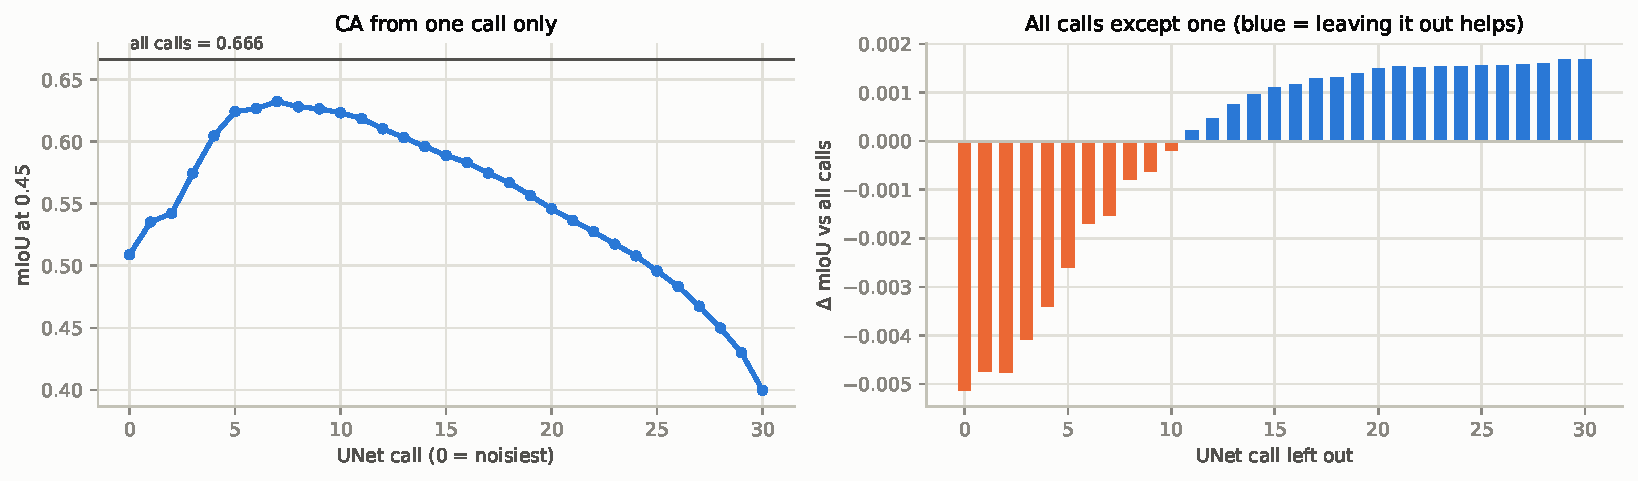
\includegraphics[width=0.8\linewidth]{evidence/figures/a2_ca_t_calls.pdf}
\caption{CA-T: CA from a single UNet call, and all calls except one.}\label{fig:rec_a2_ca_t_calls}
\end{figure}
\begin{figure}[H]\centering
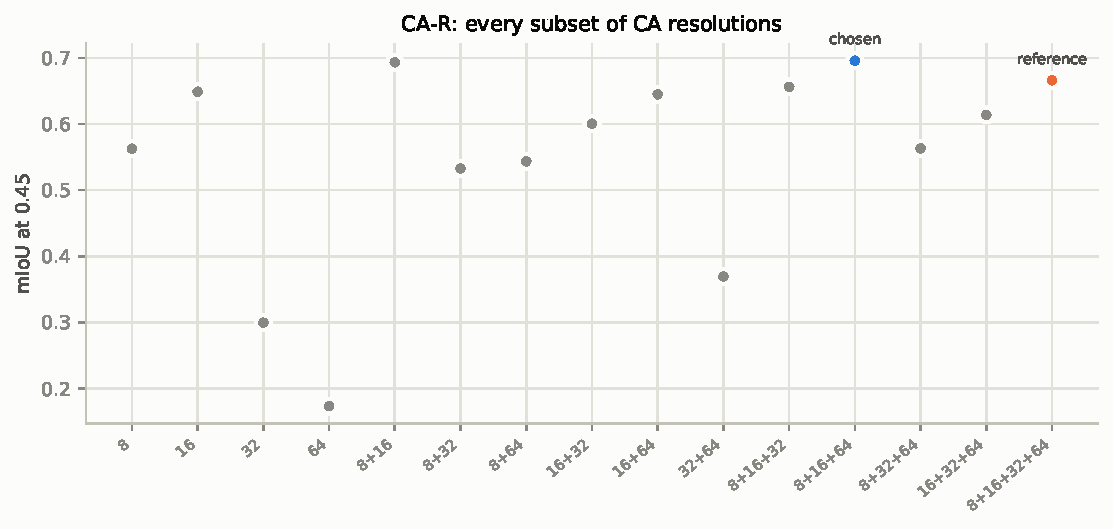
\includegraphics[width=0.55\linewidth]{evidence/figures/a2_ca_r_subsets.pdf}
\caption{CA-R: every subset of CA resolutions.}\label{fig:rec_a2_ca_r_subsets}
\end{figure}
\begin{figure}[H]\centering
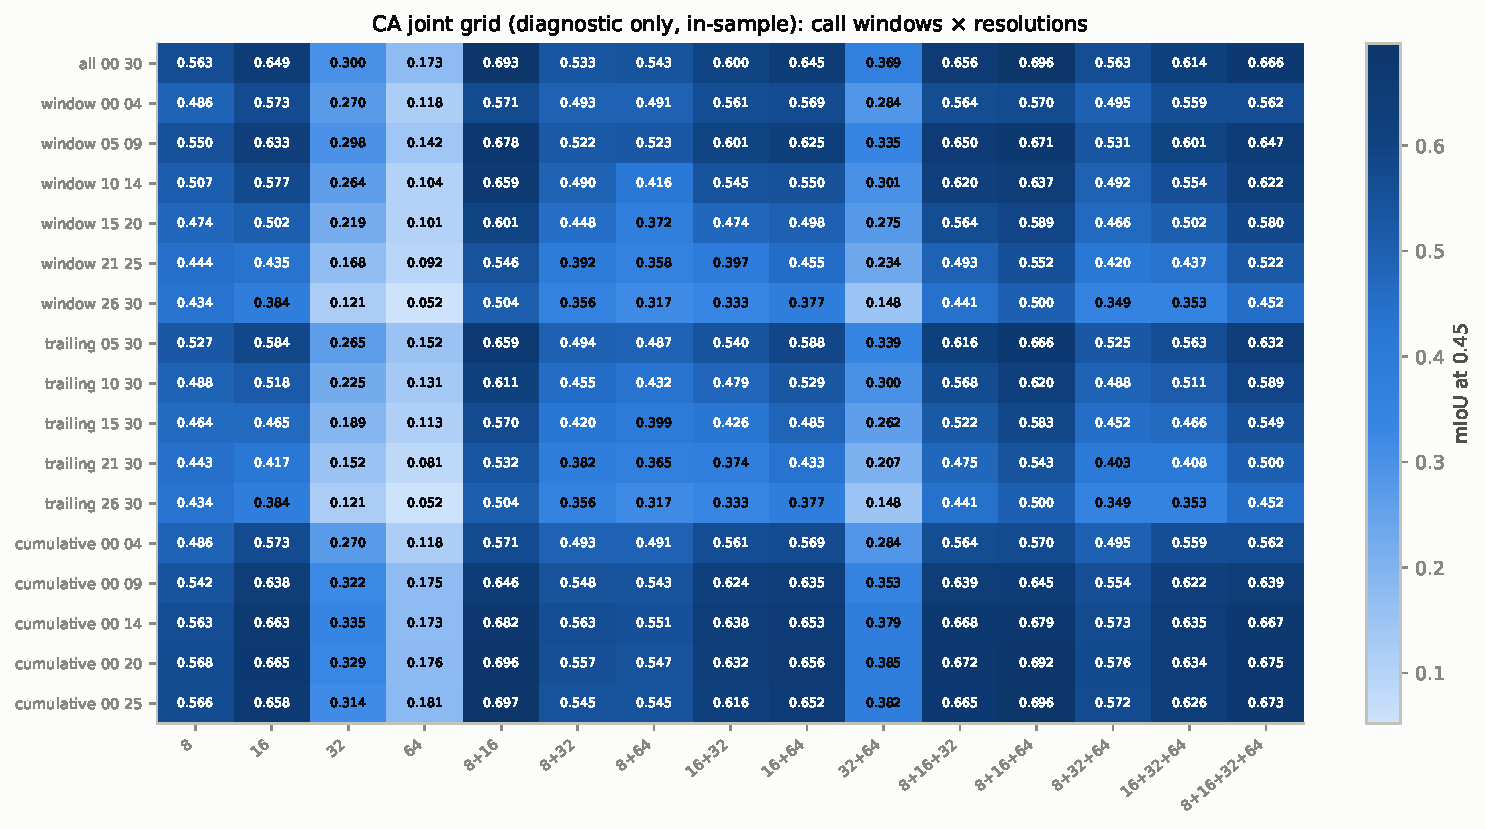
\includegraphics[width=0.75\linewidth]{evidence/figures/a2_joint_grid.pdf}
\caption{Joint grid of CA call windows and resolutions (diagnostic only).}\label{fig:rec_a2_joint_grid}
\end{figure}
\begin{figure}[H]\centering
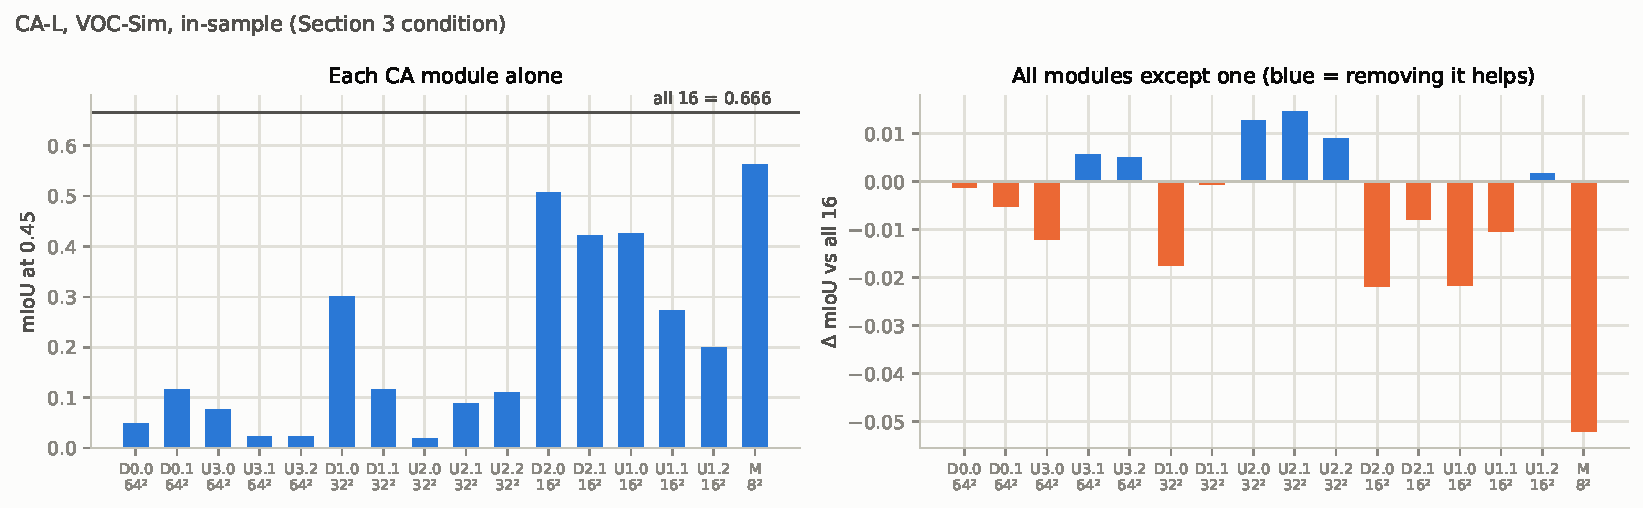
\includegraphics[width=0.8\linewidth]{evidence/figures/a1_ca_l_single_leave1.pdf}
\caption{CA-L: each CA module alone (left) and all modules except one (right).}\label{fig:rec_a1_ca_l_single_leave1}
\end{figure}
\begin{figure}[H]\centering
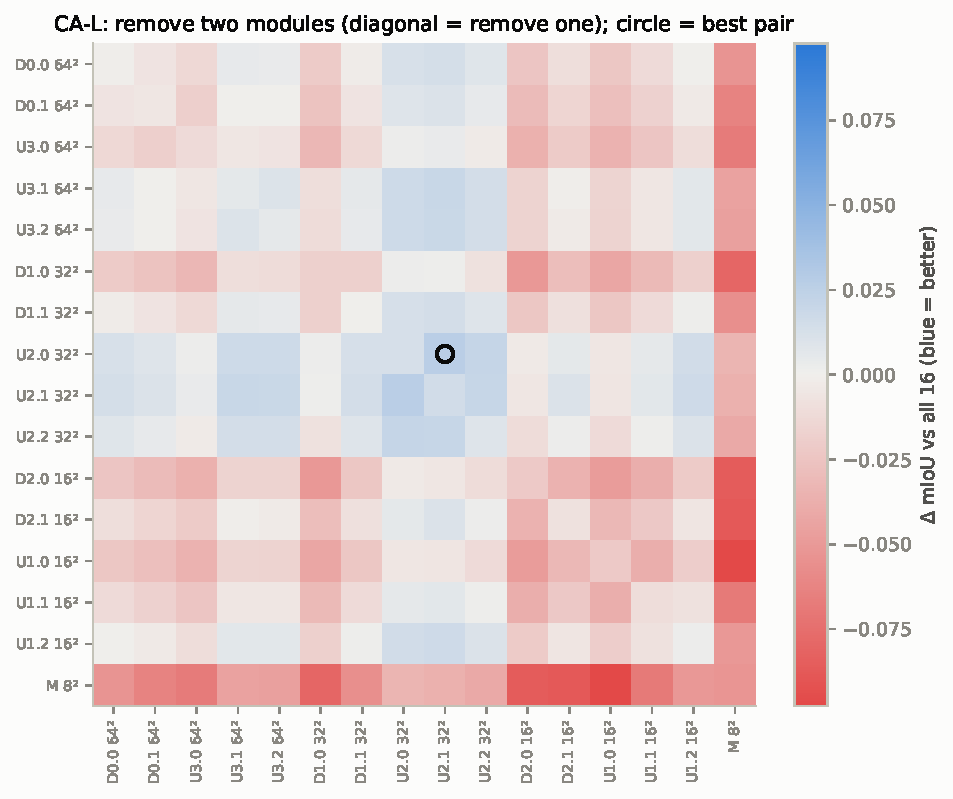
\includegraphics[width=0.55\linewidth]{evidence/figures/a1_ca_l_leave2_heatmap.pdf}
\caption{CA-L: all 120 leave-two-out configurations; the diagonal is leave-one-out.}\label{fig:rec_a1_ca_l_leave2_heatmap}
\end{figure}
\begin{figure}[H]\centering
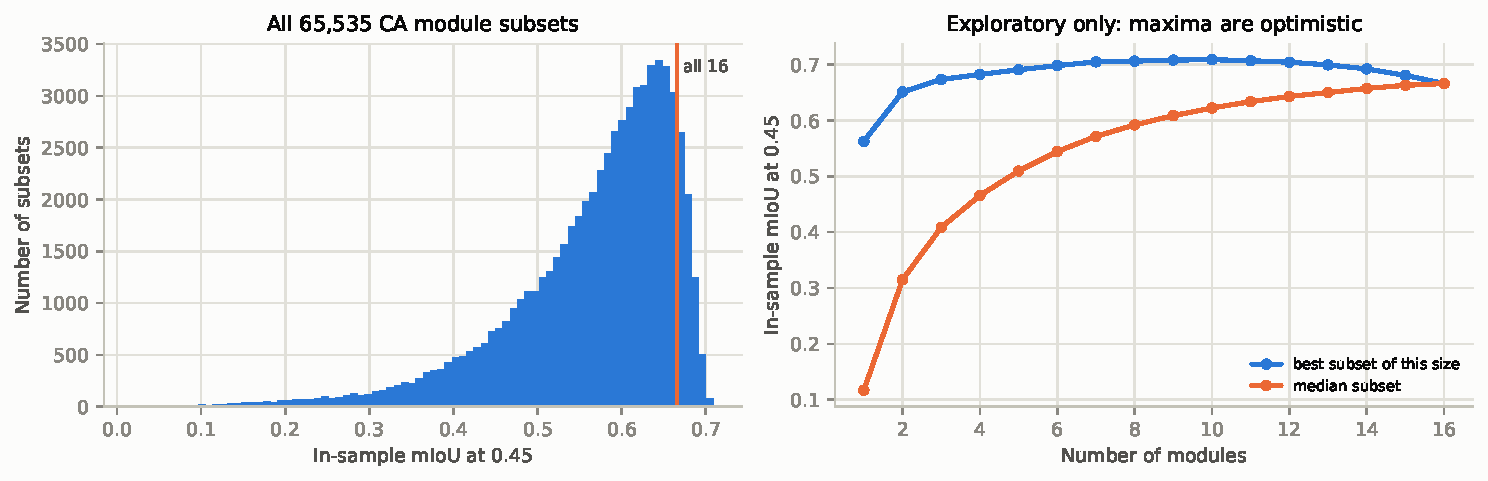
\includegraphics[width=0.8\linewidth]{evidence/figures/a1_exhaustive.pdf}
\caption{All 65{,}535 CA module subsets (exploratory; the maximum is not eligible for selection).}\label{fig:rec_a1_exhaustive}
\end{figure}
\begin{figure}[H]\centering
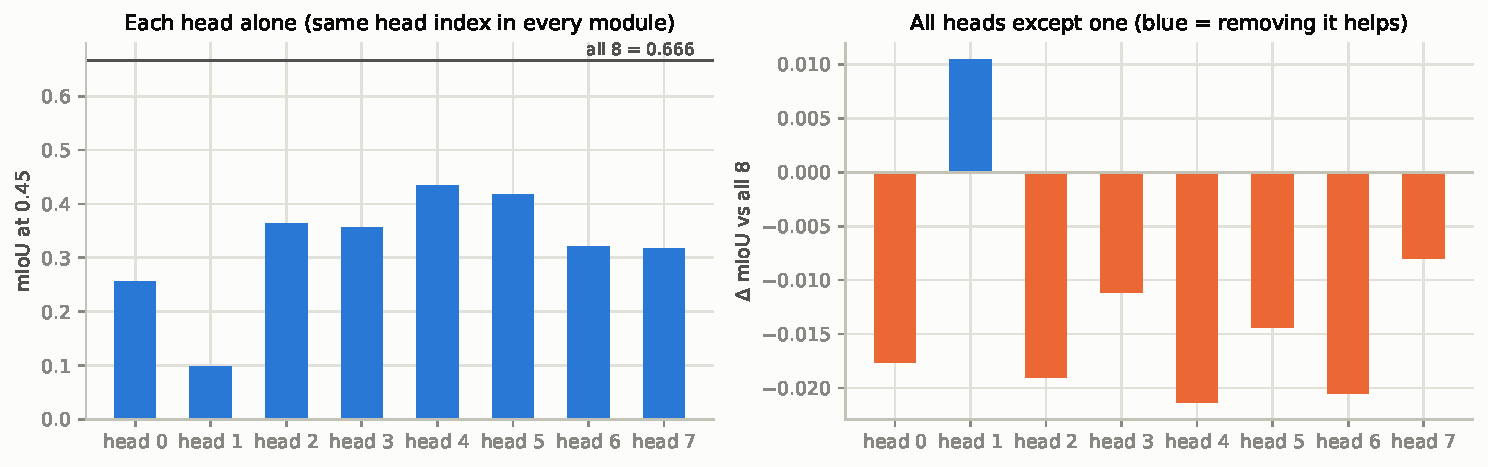
\includegraphics[width=0.8\linewidth]{evidence/figures/a1_ca_h_single_leave1.pdf}
\caption{CA-H: each head alone and all heads except one (the same head index in every module).}\label{fig:rec_a1_ca_h_single_leave1}
\end{figure}
\begin{figure}[H]\centering
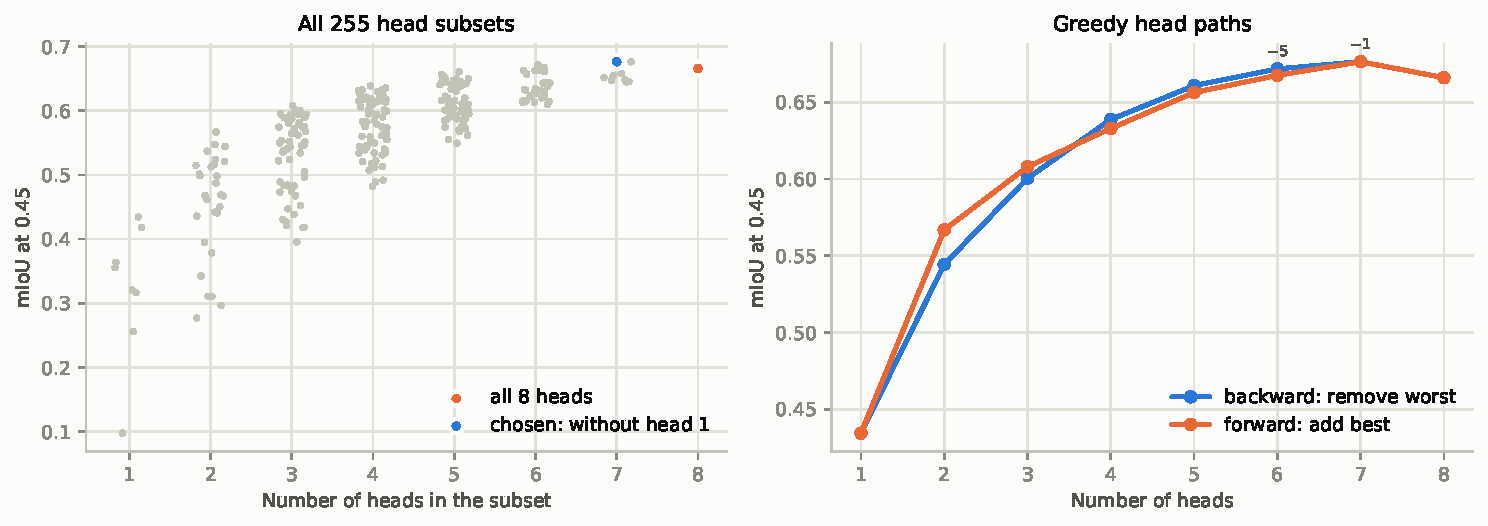
\includegraphics[width=0.8\linewidth]{evidence/figures/a1_ca_h_subsets_greedy.pdf}
\caption{CA-H: all 255 head subsets by size, and the greedy removal and addition paths.}\label{fig:rec_a1_ca_h_subsets_greedy}
\end{figure}
\begin{figure}[H]\centering
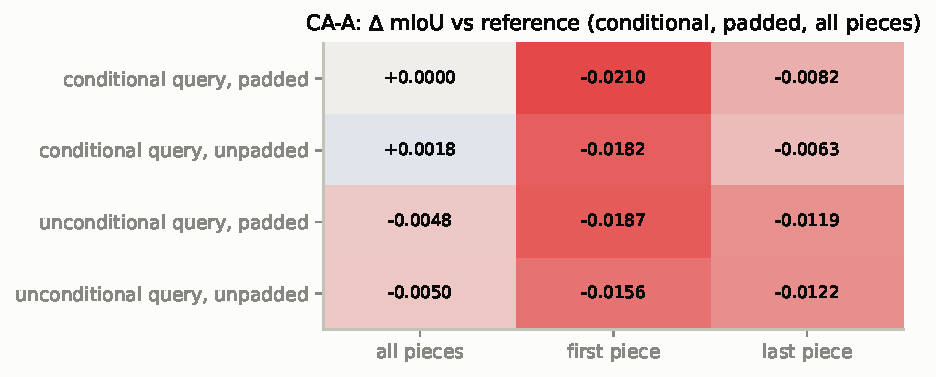
\includegraphics[width=0.5\linewidth]{evidence/figures/a1_ca_a_grid.pdf}
\caption{CA-A: change in mIoU of each attribution convention against the reference.}\label{fig:rec_a1_ca_a_grid}
\end{figure}
\begin{figure}[H]\centering
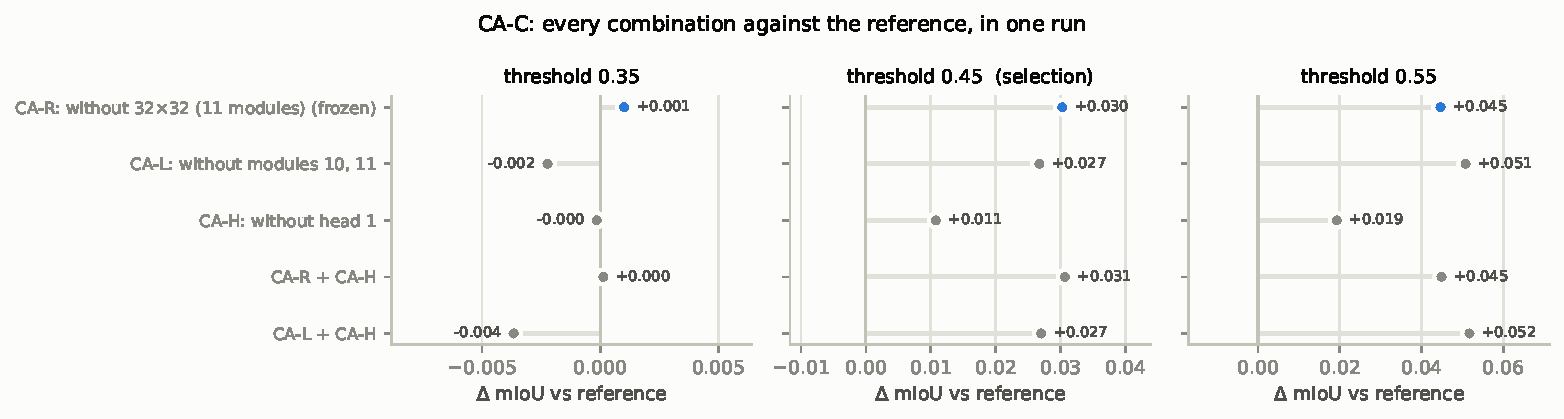
\includegraphics[width=0.8\linewidth]{evidence/figures/a3_ca_c_thresholds.pdf}
\caption{CA-C: change in mIoU of every combination against the reference at thresholds 0.35, 0.45 and 0.55 (blue = frozen).}\label{fig:rec_a3_ca_c_thresholds}
\end{figure}
\begin{figure}[H]\centering
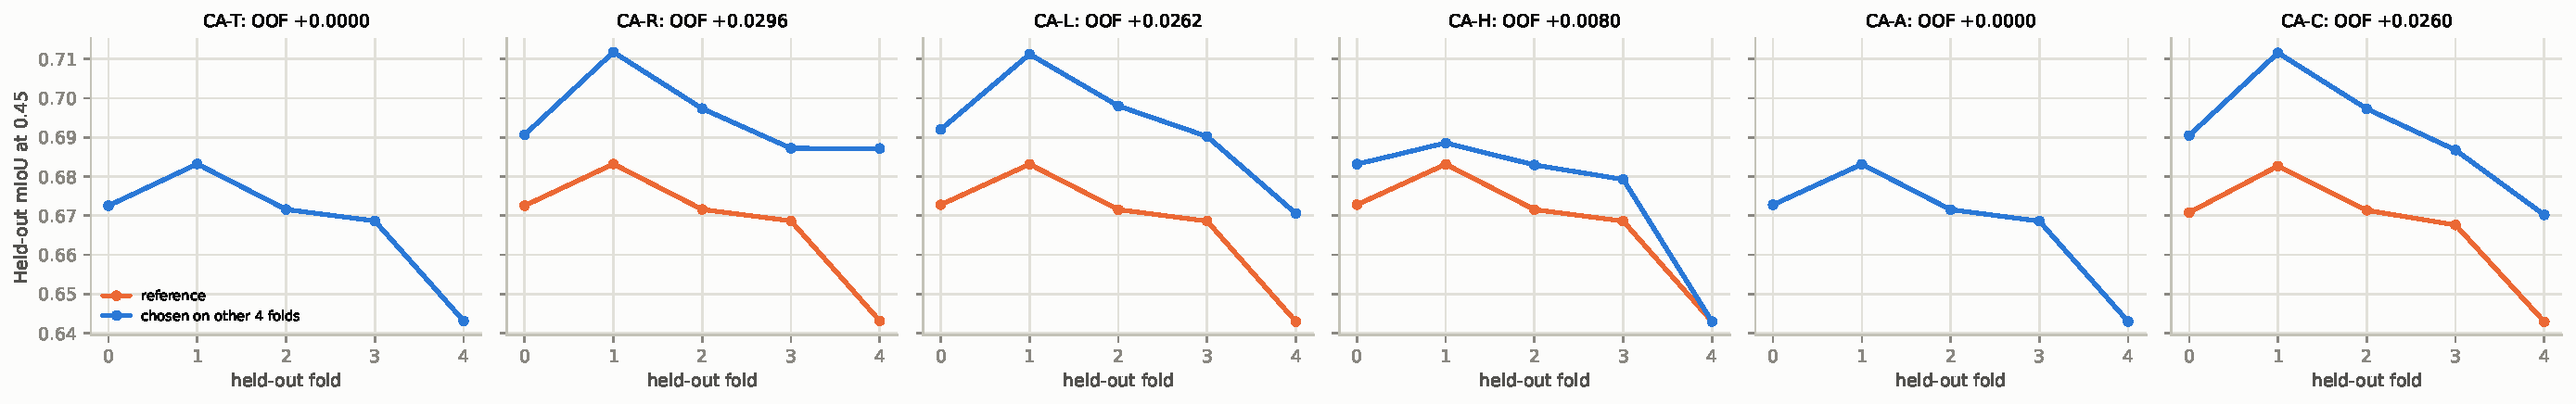
\includegraphics[width=0.8\linewidth]{evidence/figures/a_heldout_folds.pdf}
\caption{Controlled CA screens: held-out mIoU of the setting chosen on the other four folds, against the reference, per fold.}\label{fig:rec_a_heldout_folds}
\end{figure}
\begin{figure}[H]\centering
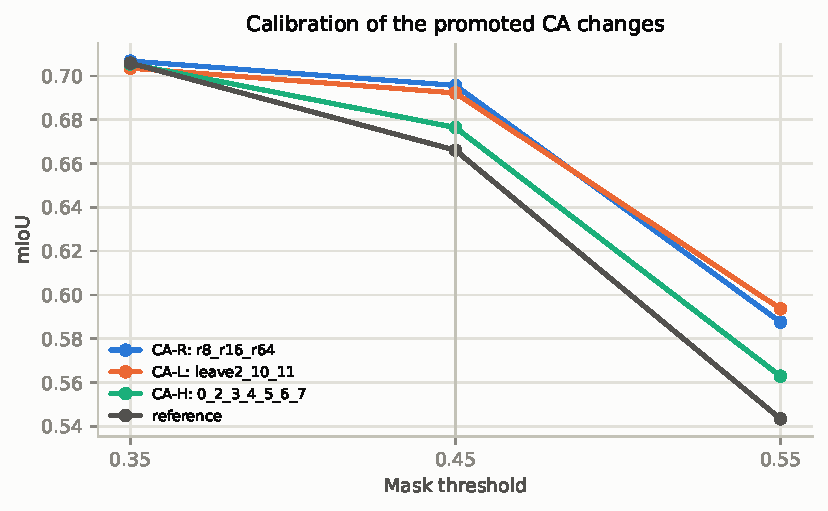
\includegraphics[width=0.45\linewidth]{evidence/figures/a_calibration.pdf}
\caption{Calibration of the promoted CA changes at thresholds 0.35, 0.45 and 0.55.}\label{fig:rec_a_calibration}
\end{figure}

\paragraph{SA module (A4--A7).}
\begin{table}[H]\centering\scriptsize\setlength{\tabcolsep}{3pt}
\begin{tabular}{>{\raggedright\arraybackslash}p{4.26cm}rrrrr>{\raggedright\arraybackslash}p{1.51cm}}
\toprule
Configuration & mIoU@0.45 & $\Delta$ vs reference & mIoU@0.35 & mIoU@0.55 & Mean AP & Fold votes \\
\midrule
reference (16 SA modules, 31 calls, 8 heads) & 0.7556 & 0.0000 & 0.7213 & 0.7466 & 0.9536 & 0/\allowbreak{}5 \\
T: call 30 only & 0.7710 & 0.0153 & 0.7465 & 0.7457 & 0.9551 & 0/\allowbreak{}5 \\
R: resolutions 8+64 & 0.7676 & 0.0119 & 0.7414 & 0.7399 & 0.9542 & 0/\allowbreak{}5 \\
L: module 15 only (U3.2) & 0.7887 & 0.0330 & 0.7691 & 0.7532 & 0.9560 & 5/\allowbreak{}5 \\
H: heads 1, 4, 6 & 0.7613 & 0.0057 & 0.7295 & 0.7470 & 0.9552 & 0/\allowbreak{}5 \\
T + R & 0.7749 & 0.0193 & 0.7659 & 0.7244 & 0.9517 & 0/\allowbreak{}5 \\
T + L & 0.7820 & 0.0264 & 0.7704 & 0.7260 & 0.9474 & 0/\allowbreak{}5 \\
T + H & 0.7732 & 0.0175 & 0.7534 & 0.7412 & 0.9563 & 0/\allowbreak{}5 \\
R + H & 0.7656 & 0.0099 & 0.7389 & 0.7343 & 0.9534 & 0/\allowbreak{}5 \\
L + H & 0.7871 & 0.0314 & 0.7637 & 0.7554 & 0.9587 & 0/\allowbreak{}5 \\
T + R + H & 0.7692 & 0.0136 & 0.7669 & 0.7098 & 0.9512 & 0/\allowbreak{}5 \\
T + L + H & 0.7825 & 0.0268 & 0.7658 & 0.7330 & 0.9514 & 0/\allowbreak{}5 \\
\bottomrule
\end{tabular}
\caption{SA-C: the combined confirmation (one run, in-sample values; fold votes from the 5-fold selection)}\label{tab:a6_sa_c}
\end{table}

\begin{table}[H]\centering\scriptsize\setlength{\tabcolsep}{3pt}
\begin{tabular}{>{\raggedright\arraybackslash}p{3.06cm}>{\raggedright\arraybackslash}p{2.11cm}>{\raggedright\arraybackslash}p{1.73cm}r}
\toprule
Component & With & Without & $\Delta$ mIoU@0.45 \\
\midrule
T within T+L+H & T + L + H & L + H & -0.0046 \\
L within T+L+H & T + L + H & T + H & 0.0093 \\
H within T+L+H & T + L + H & T + L & 0.0005 \\
R within T+R+H & T + R + H & T + H & -0.0040 \\
\bottomrule
\end{tabular}
\caption{SA-C: removing one component from the full combination (in-sample)}\label{tab:a6_sa_c_components}
\end{table}

\begin{table}[H]\centering\scriptsize\setlength{\tabcolsep}{3pt}
\begin{tabular}{r>{\raggedright\arraybackslash}p{1.40cm}rrrr}
\toprule
Held-out fold & Chosen on the other four & Train mIoU chosen & Train mIoU reference & Held-out mIoU chosen & Held-out mIoU reference \\
\midrule
0 & L: module 15 only (U3.2) & 0.7892 & 0.7580 & 0.7892 & 0.7465 \\
1 & L: module 15 only (U3.2) & 0.7825 & 0.7490 & 0.8116 & 0.7780 \\
2 & L: module 15 only (U3.2) & 0.7899 & 0.7571 & 0.7869 & 0.7518 \\
3 & L: module 15 only (U3.2) & 0.7908 & 0.7578 & 0.7825 & 0.7460 \\
4 & L: module 15 only (U3.2) & 0.7910 & 0.7559 & 0.7757 & 0.7484 \\
\bottomrule
\end{tabular}
\caption{SA-C: the choice made on each set of four folds and its held-out score}\label{tab:a6_sa_c_folds}
\end{table}

\begin{table}[H]\centering\scriptsize\setlength{\tabcolsep}{3pt}
\begin{tabular}{>{\raggedright\arraybackslash}p{2.68cm}rrr}
\toprule
Class & Reference & Module 15 only & $\Delta$ \\
\midrule
chair & 0.5289 & 0.6503 & 0.1214 \\
aeroplane & 0.7309 & 0.8450 & 0.1141 \\
bicycle & 0.6788 & 0.7471 & 0.0683 \\
boat & 0.7638 & 0.8318 & 0.0680 \\
bird & 0.7859 & 0.8531 & 0.0673 \\
bottle & 0.8126 & 0.8665 & 0.0539 \\
horse & 0.8300 & 0.8696 & 0.0396 \\
motorbike & 0.8157 & 0.8527 & 0.0370 \\
dog & 0.8692 & 0.8960 & 0.0268 \\
car & 0.8152 & 0.8420 & 0.0268 \\
train & 0.6470 & 0.6697 & 0.0227 \\
sofa & 0.9230 & 0.9447 & 0.0217 \\
dining-table & 0.4511 & 0.4677 & 0.0166 \\
cow & 0.8055 & 0.8184 & 0.0129 \\
cat & 0.7688 & 0.7816 & 0.0127 \\
bus & 0.9064 & 0.9184 & 0.0120 \\
sheep & 0.7564 & 0.7660 & 0.0096 \\
potted-plant & 0.7064 & 0.7091 & 0.0027 \\
tv & 0.7953 & 0.7768 & -0.0184 \\
person & 0.7218 & 0.6664 & -0.0554 \\
\bottomrule
\end{tabular}
\caption{SA-C: per-class IoU of the selected SA configuration against the inclusive SA reference (threshold 0.45)}\label{tab:a6_sa_c_classes}
\end{table}

\begin{table}[H]\centering\scriptsize\setlength{\tabcolsep}{3pt}
\begin{tabular}{>{\raggedright\arraybackslash}p{3.22cm}rrrrrr}
\toprule
Configuration & mIoU@0.45 & $\Delta$ vs reference & mIoU@0.35 & mIoU@0.55 & Mean AP & SD across folds \\
\midrule
all 00 30 & 0.7556 & 0.0000 & 0.7213 & 0.7466 & 0.9536 & 0.0121 \\
window 00 04 & 0.6105 & -0.1452 & 0.5513 & 0.6432 & 0.8907 & 0.0175 \\
window 05 09 & 0.7290 & -0.0266 & 0.6893 & 0.7286 & 0.9424 & 0.0130 \\
window 10 14 & 0.7569 & 0.0012 & 0.7241 & 0.7470 & 0.9535 & 0.0118 \\
window 15 20 & 0.7636 & 0.0079 & 0.7354 & 0.7477 & 0.9548 & 0.0110 \\
window 21 25 & 0.7661 & 0.0105 & 0.7412 & 0.7453 & 0.9544 & 0.0100 \\
window 26 30 & 0.7687 & 0.0131 & 0.7447 & 0.7447 & 0.9545 & 0.0098 \\
trailing 05 30 & 0.7617 & 0.0060 & 0.7318 & 0.7473 & 0.9549 & 0.0114 \\
trailing 10 30 & 0.7650 & 0.0093 & 0.7376 & 0.7474 & 0.9552 & 0.0108 \\
trailing 15 30 & 0.7663 & 0.0107 & 0.7407 & 0.7465 & 0.9549 & 0.0103 \\
trailing 21 30 & 0.7675 & 0.0119 & 0.7432 & 0.7452 & 0.9545 & 0.0098 \\
trailing 26 30 & 0.7687 & 0.0131 & 0.7447 & 0.7447 & 0.9545 & 0.0098 \\
cumulative 00 04 & 0.6105 & -0.1452 & 0.5513 & 0.6432 & 0.8907 & 0.0175 \\
cumulative 00 09 & 0.6956 & -0.0600 & 0.6390 & 0.7114 & 0.9318 & 0.0151 \\
cumulative 00 14 & 0.7276 & -0.0280 & 0.6813 & 0.7337 & 0.9454 & 0.0136 \\
cumulative 00 20 & 0.7441 & -0.0116 & 0.7042 & 0.7429 & 0.9508 & 0.0132 \\
cumulative 00 25 & 0.7510 & -0.0046 & 0.7143 & 0.7454 & 0.9526 & 0.0126 \\
\bottomrule
\end{tabular}
\caption{SA-T: call windows (in-sample; all 79 configurations, including every single call and leave-one-call-out, in controlled\_\allowbreak{}sa\_\allowbreak{}package\_\allowbreak{}a.csv)}\label{tab:a5_sa_t}
\end{table}

\begin{table}[H]\centering\scriptsize\setlength{\tabcolsep}{3pt}
\begin{tabular}{>{\raggedright\arraybackslash}p{2.87cm}rrrrrr}
\toprule
Configuration & mIoU@0.45 & $\Delta$ vs reference & mIoU@0.35 & mIoU@0.55 & Mean AP & SD across folds \\
\midrule
64 & 0.7678 & 0.0121 & 0.7474 & 0.7309 & 0.9539 & 0.0124 \\
8+64 & 0.7676 & 0.0119 & 0.7414 & 0.7399 & 0.9542 & 0.0128 \\
32+64 & 0.7627 & 0.0070 & 0.7388 & 0.7369 & 0.9550 & 0.0125 \\
8+32+64 & 0.7619 & 0.0063 & 0.7356 & 0.7399 & 0.9549 & 0.0125 \\
16+64 & 0.7578 & 0.0021 & 0.7199 & 0.7507 & 0.9531 & 0.0120 \\
16+32+64 & 0.7568 & 0.0012 & 0.7237 & 0.7457 & 0.9538 & 0.0120 \\
8+16+32+64 & 0.7556 & 0.0000 & 0.7213 & 0.7466 & 0.9536 & 0.0121 \\
8+16+64 & 0.7554 & -0.0002 & 0.7158 & 0.7516 & 0.9529 & 0.0123 \\
32 & 0.7532 & -0.0024 & 0.7275 & 0.7353 & 0.9534 & 0.0119 \\
8+32 & 0.7510 & -0.0047 & 0.7214 & 0.7387 & 0.9528 & 0.0122 \\
16+32 & 0.7434 & -0.0123 & 0.7066 & 0.7426 & 0.9503 & 0.0113 \\
8+16+32 & 0.7413 & -0.0144 & 0.7033 & 0.7430 & 0.9499 & 0.0116 \\
16 & 0.7187 & -0.0370 & 0.6749 & 0.7352 & 0.9402 & 0.0108 \\
8+16 & 0.7156 & -0.0400 & 0.6706 & 0.7343 & 0.9399 & 0.0112 \\
8 & 0.6764 & -0.0793 & 0.6237 & 0.6992 & 0.9030 & 0.0137 \\
\bottomrule
\end{tabular}
\caption{SA-R: all 15 resolution subsets (in-sample; reference 8+16+32+64)}\label{tab:a5_sa_r}
\end{table}

\begin{table}[H]\centering\scriptsize\setlength{\tabcolsep}{3pt}
\begin{tabular}{>{\raggedright\arraybackslash}p{1.40cm}>{\raggedright\arraybackslash}p{1.40cm}>{\raggedright\arraybackslash}p{1.40cm}rrr>{\raggedright\arraybackslash}p{1.40cm}>{\raggedright\arraybackslash}p{1.40cm}>{\raggedright\arraybackslash}p{1.42cm}}
\toprule
Screen & Reference & Vote winner (votes) & OOF mIoU reference & OOF mIoU choice & OOF gain & Paired $\Delta$ image IoU [95\% CI] & $\Delta$ mIoU @0.35 /\allowbreak{} 0.45 /\allowbreak{} 0.55 & Outcome \\
\midrule
SA-L & SL/\allowbreak{}all\_\allowbreak{}16 & SL/\allowbreak{}single\_\allowbreak{}15 (5/\allowbreak{}5) & 0.7553 & 0.7884 & 0.0331 & +0.0417 [+0.0365, +0.0469] & +0.0477 /\allowbreak{} +0.0331 /\allowbreak{} +0.0068 & fold vote and OOF guard passed \\
SA-H & SH/\allowbreak{}0\_\allowbreak{}1\_\allowbreak{}2\_\allowbreak{}3\_\allowbreak{}4\_\allowbreak{}5\_\allowbreak{}6\_\allowbreak{}7 & SH/\allowbreak{}1\_\allowbreak{}4\_\allowbreak{}6 (5/\allowbreak{}5) & 0.7553 & 0.7610 & 0.0057 & +0.0065 [+0.0056, +0.0074] & +0.0083 /\allowbreak{} +0.0057 /\allowbreak{} +0.0004 & fold vote and OOF guard passed \\
\bottomrule
\end{tabular}
\caption{Controlled SA package B (frozen CA seed; VOC-Sim, 5 folds, selection at 0.45). SA-C combines these with SA-T/\allowbreak{}SA-R.}\label{tab:a4_cv_summary}
\end{table}

{\scriptsize\setlength{\tabcolsep}{3pt}
\begin{longtable}{>{\raggedright\arraybackslash}p{3.73cm}rrrrrr}
\caption{SA-L: structured groups, single SA modules and leave-one-out (in-sample; all 159 in controlled\_\allowbreak{}sa\_\allowbreak{}package\_\allowbreak{}b.csv)}\label{tab:a4_sa_l}\\
\toprule
Configuration & mIoU@0.45 & $\Delta$ vs all 16 & mIoU@0.35 & mIoU@0.55 & Mean AP & SD across folds \\
\midrule
\endfirsthead
\toprule
Configuration & mIoU@0.45 & $\Delta$ vs all 16 & mIoU@0.35 & mIoU@0.55 & Mean AP & SD across folds \\
\midrule
\endhead
all\_\allowbreak{}16 & 0.7553 & 0.0000 & 0.7212 & 0.7463 & 0.9535 & 0.0124 \\
non\_\allowbreak{}middle\_\allowbreak{}15 & 0.7565 & 0.0012 & 0.7237 & 0.7454 & 0.9537 & 0.0122 \\
down\_\allowbreak{}only & 0.7472 & -0.0081 & 0.7038 & 0.7503 & 0.9507 & 0.0124 \\
middle\_\allowbreak{}only & 0.6763 & -0.0790 & 0.6236 & 0.6990 & 0.9029 & 0.0138 \\
up\_\allowbreak{}only & 0.7556 & 0.0003 & 0.7301 & 0.7357 & 0.9525 & 0.0120 \\
down\_\allowbreak{}middle & 0.7448 & -0.0105 & 0.6990 & 0.7534 & 0.9506 & 0.0126 \\
middle\_\allowbreak{}up & 0.7539 & -0.0014 & 0.7261 & 0.7376 & 0.9523 & 0.0121 \\
only 00 D0.0 (64$^2$) & 0.7311 & -0.0243 & 0.6994 & 0.6993 & 0.9292 & 0.0149 \\
only 01 D0.1 (64$^2$) & 0.7458 & -0.0095 & 0.7121 & 0.7224 & 0.9384 & 0.0142 \\
only 02 D1.0 (32$^2$) & 0.7371 & -0.0182 & 0.6891 & 0.7442 & 0.9485 & 0.0127 \\
only 03 D1.1 (32$^2$) & 0.7412 & -0.0141 & 0.7007 & 0.7425 & 0.9500 & 0.0113 \\
only 04 D2.0 (16$^2$) & 0.7116 & -0.0437 & 0.6703 & 0.7232 & 0.9400 & 0.0132 \\
only 05 D2.1 (16$^2$) & 0.7112 & -0.0442 & 0.6671 & 0.7274 & 0.9403 & 0.0110 \\
only 06 M (8$^2$) & 0.6763 & -0.0790 & 0.6236 & 0.6990 & 0.9029 & 0.0138 \\
only 07 U1.0 (16$^2$) & 0.7203 & -0.0351 & 0.6686 & 0.7411 & 0.9395 & 0.0114 \\
only 08 U1.1 (16$^2$) & 0.7125 & -0.0428 & 0.6714 & 0.7253 & 0.9280 & 0.0107 \\
only 09 U1.2 (16$^2$) & 0.7155 & -0.0398 & 0.6718 & 0.7316 & 0.9368 & 0.0101 \\
only 10 U2.0 (32$^2$) & 0.7387 & -0.0166 & 0.7303 & 0.7017 & 0.9494 & 0.0112 \\
only 11 U2.1 (32$^2$) & 0.7416 & -0.0138 & 0.7325 & 0.7045 & 0.9473 & 0.0110 \\
only 12 U2.2 (32$^2$) & 0.7698 & 0.0145 & 0.7375 & 0.7532 & 0.9557 & 0.0120 \\
only 13 U3.0 (64$^2$) & 0.7397 & -0.0156 & 0.7394 & 0.6857 & 0.9476 & 0.0127 \\
only 14 U3.1 (64$^2$) & 0.7546 & -0.0007 & 0.7440 & 0.7120 & 0.9526 & 0.0130 \\
only 15 U3.2 (64$^2$) & 0.7884 & 0.0331 & 0.7689 & 0.7531 & 0.9559 & 0.0123 \\
without 00 D0.0 & 0.7536 & -0.0018 & 0.7201 & 0.7448 & 0.9531 & 0.0121 \\
without 01 D0.1 & 0.7533 & -0.0020 & 0.7199 & 0.7442 & 0.9532 & 0.0124 \\
without 02 D1.0 & 0.7556 & 0.0003 & 0.7224 & 0.7455 & 0.9534 & 0.0123 \\
without 03 D1.1 & 0.7556 & 0.0003 & 0.7216 & 0.7460 & 0.9534 & 0.0124 \\
without 04 D2.0 & 0.7570 & 0.0016 & 0.7236 & 0.7462 & 0.9537 & 0.0123 \\
without 05 D2.1 & 0.7566 & 0.0012 & 0.7233 & 0.7459 & 0.9537 & 0.0123 \\
without 06 M & 0.7565 & 0.0012 & 0.7237 & 0.7454 & 0.9537 & 0.0122 \\
without 07 U1.0 & 0.7559 & 0.0005 & 0.7233 & 0.7449 & 0.9537 & 0.0125 \\
without 08 U1.1 & 0.7571 & 0.0018 & 0.7247 & 0.7453 & 0.9542 & 0.0126 \\
without 09 U1.2 & 0.7565 & 0.0011 & 0.7233 & 0.7455 & 0.9537 & 0.0124 \\
without 10 U2.0 & 0.7560 & 0.0006 & 0.7193 & 0.7494 & 0.9535 & 0.0125 \\
without 11 U2.1 & 0.7556 & 0.0003 & 0.7193 & 0.7489 & 0.9537 & 0.0125 \\
without 12 U2.2 & 0.7540 & -0.0013 & 0.7195 & 0.7454 & 0.9531 & 0.0123 \\
without 13 U3.0 & 0.7550 & -0.0003 & 0.7177 & 0.7502 & 0.9537 & 0.0124 \\
without 14 U3.1 & 0.7543 & -0.0011 & 0.7181 & 0.7482 & 0.9532 & 0.0122 \\
without 15 U3.2 & 0.7517 & -0.0036 & 0.7171 & 0.7440 & 0.9526 & 0.0123 \\
\bottomrule
\end{longtable}}

\begin{table}[H]\centering\scriptsize\setlength{\tabcolsep}{3pt}
\begin{tabular}{>{\raggedright\arraybackslash}p{5.47cm}rrrrr}
\toprule
Configuration & mIoU@0.45 & $\Delta$ vs SA reference & mIoU@0.35 & mIoU@0.55 & Mean AP \\
\midrule
frozen CA seed alone (no SA) & 0.6956 & -0.0597 & 0.7067 & 0.5877 & 0.9131 \\
SA reference: all 16 SA modules, 8 heads, y = A x & 0.7553 & 0.0000 & 0.7212 & 0.7463 & 0.9535 \\
operator check: y = Aᵀx & 0.4741 & -0.2813 & 0.5914 & 0.3273 & 0.9179 \\
SA-L choice: single\_\allowbreak{}15 & 0.7884 & 0.0331 & 0.7689 & 0.7531 & 0.9559 \\
SA-H choice: heads 1, 4, 6 & 0.7610 & 0.0057 & 0.7294 & 0.7467 & 0.9552 \\
\bottomrule
\end{tabular}
\caption{SA package B: what one SA pass adds to the frozen CA seed, the transposed operator, and the two choices (in-sample)}\label{tab:a4_checks}
\end{table}

\begin{table}[H]\centering\scriptsize\setlength{\tabcolsep}{3pt}
\begin{tabular}{rrrr>{\raggedright\arraybackslash}p{3.82cm}}
\toprule
Head & Alone & All but this head & $\Delta$ vs all 8 & Folds retaining it \\
\midrule
0 & 0.7541 & 0.7552 & -0.0002 & 0/\allowbreak{}5 \\
1 & 0.7577 & 0.7548 & -0.0005 & 5/\allowbreak{}5 \\
2 & 0.7512 & 0.7558 & 0.0005 & 0/\allowbreak{}5 \\
3 & 0.7486 & 0.7561 & 0.0007 & 0/\allowbreak{}5 \\
4 & 0.7625 & 0.7540 & -0.0014 & 5/\allowbreak{}5 \\
5 & 0.7460 & 0.7567 & 0.0014 & 0/\allowbreak{}5 \\
6 & 0.7605 & 0.7544 & -0.0010 & 5/\allowbreak{}5 \\
7 & 0.7513 & 0.7555 & 0.0002 & 0/\allowbreak{}5 \\
\bottomrule
\end{tabular}
\caption{SA-H: each SA head alone and leave-one-out (in-sample mIoU at 0.45), and fold retention}\label{tab:a4_sa_h_heads}
\end{table}

\begin{table}[H]\centering\scriptsize\setlength{\tabcolsep}{3pt}
\begin{tabular}{>{\raggedright\arraybackslash}p{2.49cm}rrrrrr}
\toprule
Head subset & Heads & mIoU@0.45 & $\Delta$ vs all 8 & mIoU@0.35 & mIoU@0.55 & Mean AP \\
\midrule
4 & 1 & 0.7625 & 0.0072 & 0.7301 & 0.7473 & 0.9564 \\
4 6 & 2 & 0.7623 & 0.0070 & 0.7288 & 0.7498 & 0.9550 \\
1 4 6 & 3 & 0.7610 & 0.0057 & 0.7294 & 0.7467 & 0.9552 \\
1 4 & 2 & 0.7606 & 0.0053 & 0.7302 & 0.7446 & 0.9561 \\
6 & 1 & 0.7605 & 0.0052 & 0.7255 & 0.7499 & 0.9523 \\
0 4 6 & 3 & 0.7604 & 0.0051 & 0.7238 & 0.7522 & 0.9544 \\
0 1 4 6 & 4 & 0.7600 & 0.0047 & 0.7258 & 0.7494 & 0.9547 \\
4 6 7 & 3 & 0.7597 & 0.0044 & 0.7278 & 0.7463 & 0.9544 \\
0 1 4 & 3 & 0.7594 & 0.0040 & 0.7249 & 0.7490 & 0.9553 \\
1 6 & 2 & 0.7594 & 0.0040 & 0.7281 & 0.7453 & 0.9539 \\
\bottomrule
\end{tabular}
\caption{SA-H: the 10 best of 255 SA head subsets (in-sample; all 255 in controlled\_\allowbreak{}sa\_\allowbreak{}package\_\allowbreak{}b.csv)}\label{tab:a4_sa_h_top}
\end{table}


\begin{figure}[H]\centering
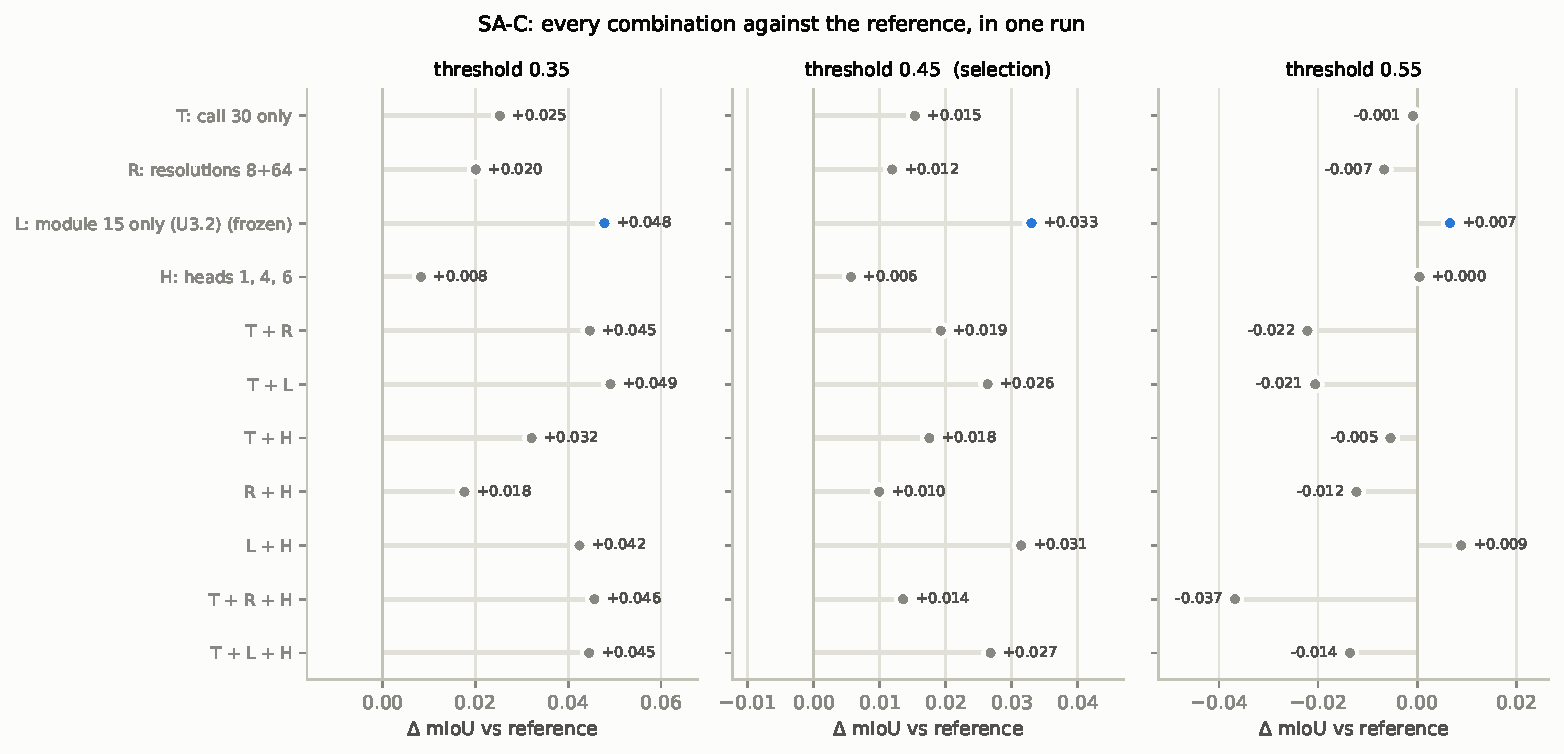
\includegraphics[width=0.8\linewidth]{evidence/figures/a6_sa_c_thresholds.pdf}
\caption{SA-C: change in mIoU of every combination against the SA reference at thresholds 0.35, 0.45 and 0.55 (blue = frozen).}\label{fig:rec_a6_sa_c_thresholds}
\end{figure}
\begin{figure}[H]\centering
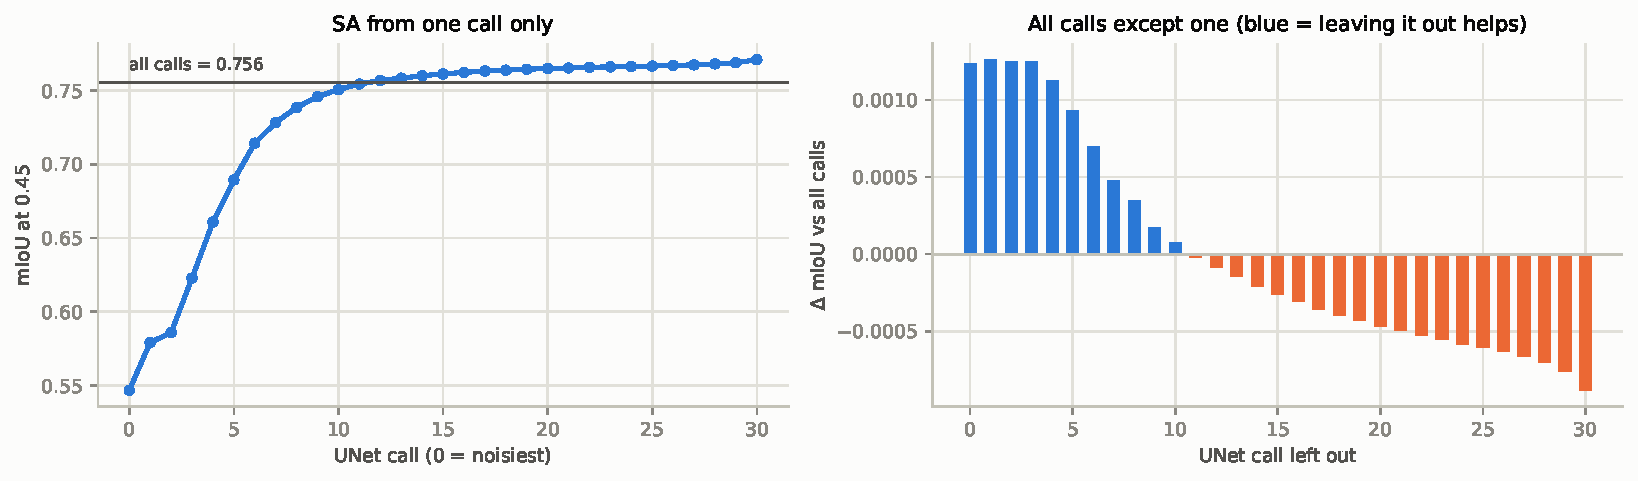
\includegraphics[width=0.8\linewidth]{evidence/figures/a5_sa_t_calls.pdf}
\caption{SA-T: SA from a single UNet call, and all calls except one.}\label{fig:rec_a5_sa_t_calls}
\end{figure}
\begin{figure}[H]\centering
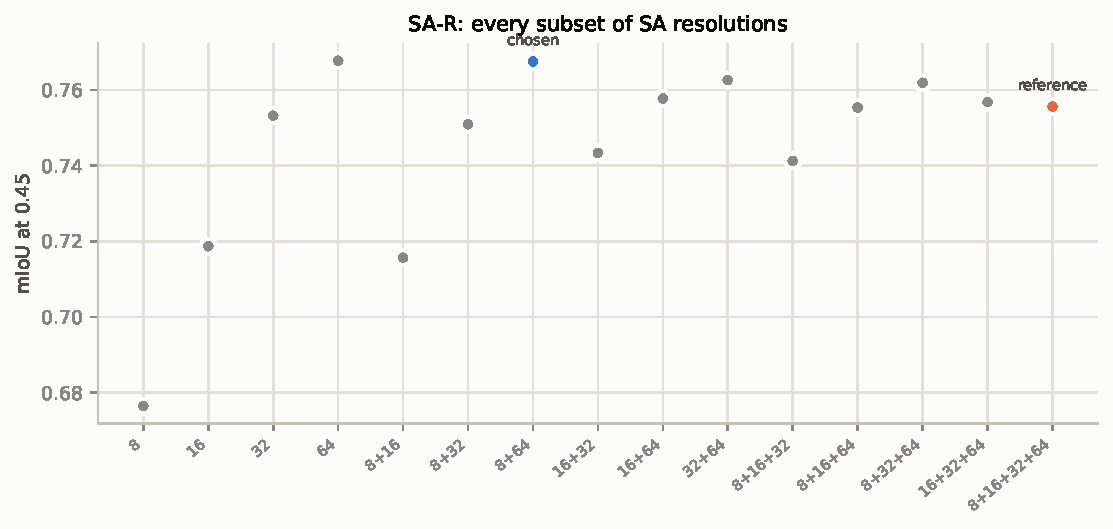
\includegraphics[width=0.55\linewidth]{evidence/figures/a5_sa_r_subsets.pdf}
\caption{SA-R: every subset of SA resolutions.}\label{fig:rec_a5_sa_r_subsets}
\end{figure}
\begin{figure}[H]\centering
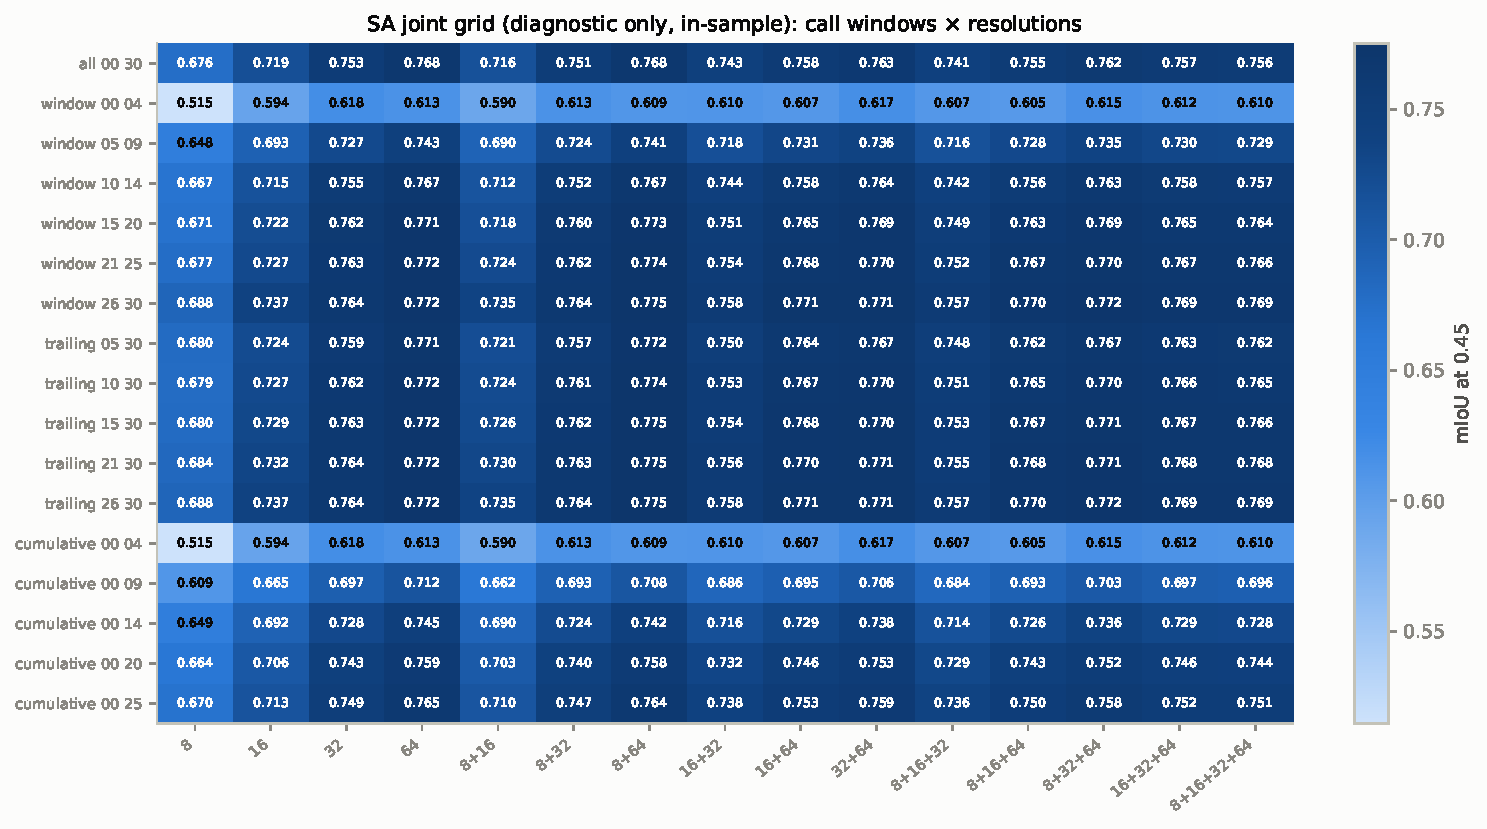
\includegraphics[width=0.75\linewidth]{evidence/figures/a5_joint_grid.pdf}
\caption{SA joint grid of call windows and resolutions (diagnostic only).}\label{fig:rec_a5_joint_grid}
\end{figure}
\begin{figure}[H]\centering
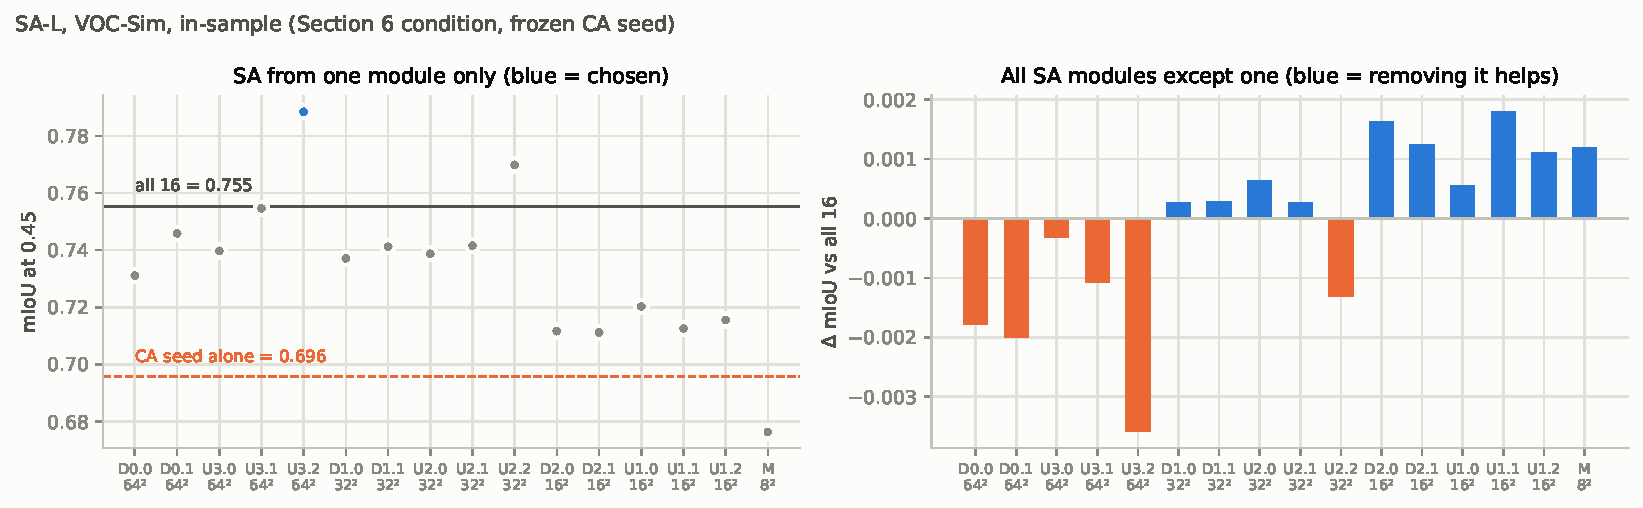
\includegraphics[width=0.8\linewidth]{evidence/figures/a4_sa_l_single_leave1.pdf}
\caption{SA-L: SA from one module only, and all SA modules except one (frozen CA seed).}\label{fig:rec_a4_sa_l_single_leave1}
\end{figure}
\begin{figure}[H]\centering
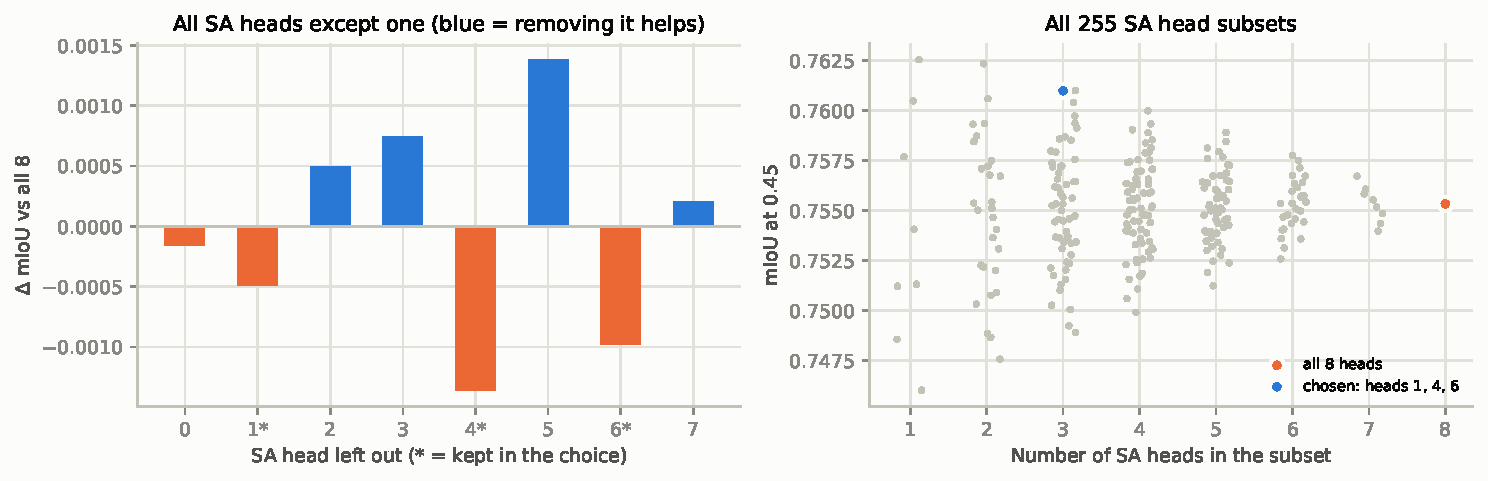
\includegraphics[width=0.8\linewidth]{evidence/figures/a4_sa_h.pdf}
\caption{SA-H: leaving out one SA head, and all 255 SA head subsets by size.}\label{fig:rec_a4_sa_h}
\end{figure}
\begin{figure}[H]\centering
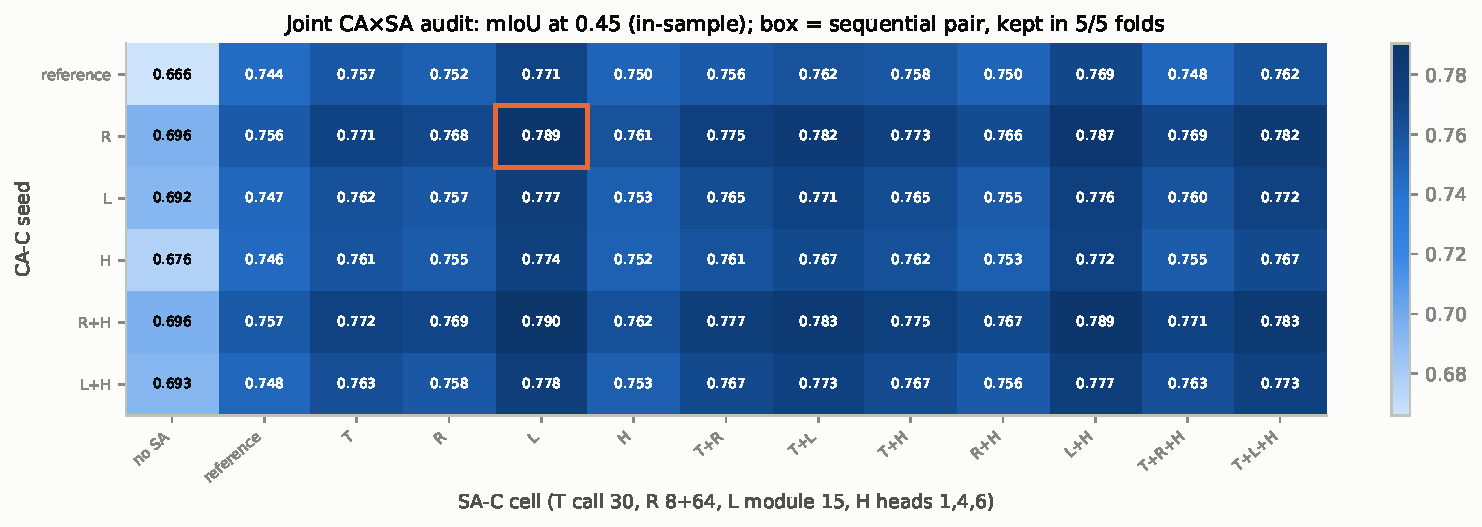
\includegraphics[width=0.8\linewidth]{evidence/figures/a7_joint_audit.pdf}
\caption{Joint CA$\times$SA audit: mIoU of all 78 cells (in-sample); the box is the frozen pair.}\label{fig:rec_a7_joint_audit}
\end{figure}

\paragraph{Propagation, refinement and tokens (A8--A12).}
\begin{table}[H]\centering\scriptsize\setlength{\tabcolsep}{3pt}
\begin{tabular}{>{\raggedright\arraybackslash}p{1.40cm}>{\raggedright\arraybackslash}p{1.40cm}rrr>{\raggedright\arraybackslash}p{1.51cm}>{\raggedright\arraybackslash}p{1.40cm}r>{\raggedright\arraybackslash}p{1.40cm}}
\toprule
Screen & Fold choice (votes) & OOF mIoU REF & OOF mIoU choice & OOF gain & Paired $\Delta$ image IoU [95\% CI]; better/\allowbreak{}worse & $\Delta$ mIoU @0.35 /\allowbreak{} 0.45 /\allowbreak{} 0.55 & Candidates & Outcome \\
\midrule
P1 observation-wise powers & P1/\allowbreak{}obs\_\allowbreak{}n2 (4/\allowbreak{}5) & 0.7875 & 0.7991 & 0.0116 & +0.0140 [+0.0097, +0.0180]; 359/\allowbreak{}131 & +0.0087 /\allowbreak{} +0.0121 /\allowbreak{} +0.0243 & 3 & fold vote and OOF guard passed \\
W3 average-before powers & REF/\allowbreak{}one\_\allowbreak{}pass (4/\allowbreak{}5) & 0.7875 & 0.7875 & -0.0000 & --- & --- & 4 & reference won the fold vote \\
P2 observation-wise restart & REF/\allowbreak{}one\_\allowbreak{}pass (4/\allowbreak{}5) & 0.7875 & 0.7877 & 0.0002 & --- & --- & 12 & reference won the fold vote \\
P2 average-before restart & REF/\allowbreak{}one\_\allowbreak{}pass (5/\allowbreak{}5) & 0.7875 & 0.7875 & 0.0000 & --- & --- & 12 & reference won the fold vote \\
P6 sparse affinity & REF/\allowbreak{}one\_\allowbreak{}pass (5/\allowbreak{}5) & 0.7875 & 0.7875 & 0.0000 & --- & --- & 7 & reference won the fold vote \\
\bottomrule
\end{tabular}
\caption{Phase 3 propagation package (Codex) (VOC-Sim, 5 folds; method parameter and threshold chosen on the training folds)}\label{tab:a8_cv_summary}
\end{table}

\begin{table}[H]\centering\scriptsize\setlength{\tabcolsep}{3pt}
\begin{tabular}{>{\raggedright\arraybackslash}p{1.40cm}>{\raggedright\arraybackslash}p{1.40cm}rrr>{\raggedright\arraybackslash}p{1.60cm}>{\raggedright\arraybackslash}p{1.40cm}r>{\raggedright\arraybackslash}p{1.40cm}}
\toprule
Screen & Fold choice (votes) & OOF mIoU REF & OOF mIoU choice & OOF gain & Paired $\Delta$ image IoU [95\% CI]; better/\allowbreak{}worse & $\Delta$ mIoU @0.35 /\allowbreak{} 0.45 /\allowbreak{} 0.55 & Candidates & Outcome \\
\midrule
P4 residual mix & REF/\allowbreak{}one\_\allowbreak{}pass (5/\allowbreak{}5) & 0.7875 & 0.7875 & 0.0000 & --- & --- & 4 & reference won the fold vote \\
F3/\allowbreak{}F4 gating & REF/\allowbreak{}one\_\allowbreak{}pass (5/\allowbreak{}5) & 0.7875 & 0.7875 & 0.0000 & --- & --- & 2 & reference won the fold vote \\
N2-N4 calibration & REF/\allowbreak{}one\_\allowbreak{}pass (5/\allowbreak{}5) & 0.7875 & 0.7875 & 0.0000 & --- & --- & 3 & reference won the fold vote \\
R2 DenseCRF & R2/\allowbreak{}crf (5/\allowbreak{}5) & 0.7875 & 0.8049 & 0.0175 & +0.0222 [+0.0185, +0.0260]; 361/\allowbreak{}129 & +0.0215 /\allowbreak{} +0.0141 /\allowbreak{} +0.0063 & 1 & fold vote and OOF guard passed \\
\bottomrule
\end{tabular}
\caption{Phase 3 fusion and calibration package (VOC-Sim, 5 folds; method parameter and threshold chosen on the training folds)}\label{tab:a9_cv_summary}
\end{table}

\begin{table}[H]\centering\scriptsize\setlength{\tabcolsep}{3pt}
\begin{tabular}{>{\raggedright\arraybackslash}p{1.57cm}>{\raggedright\arraybackslash}p{1.40cm}rrr>{\raggedright\arraybackslash}p{1.40cm}>{\raggedright\arraybackslash}p{1.40cm}r>{\raggedright\arraybackslash}p{1.40cm}}
\toprule
Screen & Fold choice (votes) & OOF mIoU REF & OOF mIoU choice & OOF gain & Paired $\Delta$ image IoU [95\% CI]; better/\allowbreak{}worse & $\Delta$ mIoU @0.35 /\allowbreak{} 0.45 /\allowbreak{} 0.55 & Candidates & Outcome \\
\midrule
B1 released token, OVAM form (unconditional query) & TU/\allowbreak{}REF (5/\allowbreak{}5) & 0.7873 & 0.8428 & 0.0555 & +0.0470 [+0.0380, +0.0560]; 369/\allowbreak{}121 & +0.0324 /\allowbreak{} +0.0518 /\allowbreak{} +0.0819 & 1 & fold vote and OOF guard passed \\
B1 released token, conditional query & TC/\allowbreak{}REF (5/\allowbreak{}5) & 0.7873 & 0.8507 & 0.0634 & +0.0529 [+0.0440, +0.0621]; 375/\allowbreak{}115 & +0.0414 /\allowbreak{} +0.0596 /\allowbreak{} +0.0852 & 1 & fold vote and OOF guard passed \\
\bottomrule
\end{tabular}
\caption{Token track B1 (released token vs class word on REF) (VOC-Sim, 5 folds; method parameter and threshold chosen on the training folds)}\label{tab:a11_cv_summary}
\end{table}

\begin{table}[H]\centering\scriptsize\setlength{\tabcolsep}{3pt}
\begin{tabular}{>{\raggedright\arraybackslash}p{1.92cm}rrr}
\toprule
Pipeline & Class word & Token, OVAM form & Token, conditional \\
\midrule
seed & 0.6956 & 0.7893 & 0.7962 \\
REF & 0.7884 & 0.8402 & 0.8480 \\
P1 & 0.8006 & 0.8444 & 0.8519 \\
R2 & 0.8024 & 0.8567 & 0.8650 \\
P1+R2 & 0.8132 & 0.8589 & 0.8664 \\
\bottomrule
\end{tabular}
\caption{Token track: class word vs OVAM's released token on every pipeline (mIoU at 0.45, in-sample; OOF values in protocol Section 50)}\label{tab:a11_token_pipelines}
\end{table}

\begin{table}[H]\centering\scriptsize\setlength{\tabcolsep}{3pt}
\begin{tabular}{>{\raggedright\arraybackslash}p{5.91cm}>{\raggedright\arraybackslash}p{1.40cm}rr}
\toprule
Token & Cell & VOC-Sim mIoU (T-C, 0.475) & Images \\
\midrule
released (OVAM, 2-3 supports) & REL & 0.8653 & 490 \\
support 1 & A1 & 0.8333 & 490 \\
support 2 & A2 & 0.8630 & 490 \\
support 3 (19 classes) & A3 & 0.8451 & 468 \\
supports 1+2 & A12 & 0.8689 & 490 \\
supports 1+3 (19 classes) & A13 & 0.8589 & 468 \\
supports 2+3 (19 classes) & A23 & 0.8713 & 468 \\
all supports & AALL & 0.8684 & 490 \\
fold-safe one-support (B2b) & B2B & 0.8564 & 490 \\
\bottomrule
\end{tabular}
\caption{A12: retrained tokens in the frozen T-C pipeline (linear-objective variant of OVAM's recipe)}\label{tab:a12_token_learning}
\end{table}

\begin{table}[H]\centering\scriptsize\setlength{\tabcolsep}{3pt}
\begin{tabular}{>{\raggedright\arraybackslash}p{4.75cm}rr>{\raggedright\arraybackslash}p{2.63cm}r}
\toprule
Comparison & $\Delta$ mIoU & Paired $\Delta$ image IoU & 95\% CI & Classes improved \\
\midrule
all supports vs released, VOC-Sim & 0.0032 & 0.0018 & [-0.0033, +0.0064] & 14 \\
fold-safe one-support vs released, VOC-Sim & -0.0089 & -0.0035 & [-0.0119, +0.0042] & 5 \\
all supports vs released, COCO-Cap & 0.0075 & 0.0096 & [+0.0039, +0.0154] & 14 \\
\bottomrule
\end{tabular}
\caption{A12: retrained against released tokens (paired bootstrap over images)}\label{tab:a12_comparisons}
\end{table}

\begin{table}[H]\centering\scriptsize\setlength{\tabcolsep}{3pt}
\begin{tabular}{>{\raggedright\arraybackslash}p{3.33cm}>{\raggedright\arraybackslash}p{3.28cm}r}
\toprule
Attention objective (unconditional, no middle block) & Epoch-0 loss vs OVAM, median abs. diff. (57 images) & Token cosine to OVAM after 800 epochs (6 images) \\
\midrule
token softmax (OVAM's library default) & 1.8e-06 & 0.9961 \\
linear (B2 recipe) & 1.8e-02 & 0.8731 \\
\bottomrule
\end{tabular}
\caption{A12: which attention objective reproduces OVAM's released optimization (protocol Section 69)}\label{tab:a12_recipe_audit}
\end{table}

\begin{table}[H]\centering\scriptsize\setlength{\tabcolsep}{3pt}
\begin{tabular}{>{\raggedright\arraybackslash}p{1.92cm}rrrr}
\toprule
Passes & mIoU@0.45 & Recall & Precision & FP per object pixel \\
\midrule
seed & 0.6957 & 0.8220 & 0.8434 & 0.1996 \\
1 pass & 0.7887 & 0.9123 & 0.8650 & 0.1827 \\
2 passes & 0.8007 & 0.9239 & 0.8655 & 0.1822 \\
3 passes & 0.8014 & 0.9271 & 0.8624 & 0.1874 \\
4 passes & 0.8004 & 0.9291 & 0.8589 & 0.1936 \\
\bottomrule
\end{tabular}
\caption{AN1: error decomposition by propagation pass (VOC-Sim, class word, threshold 0.45, in-sample)}\label{tab:an1_by_pass}
\end{table}

\begin{table}[H]\centering\scriptsize\setlength{\tabcolsep}{3pt}
\begin{tabular}{>{\raggedright\arraybackslash}p{2.15cm}rrr}
\toprule
Setting & Seed recall & Mean second-pass gain (image IoU) & Spearman: seed recall vs gain \\
\midrule
voc\_\allowbreak{}word & 0.8403 & 0.0127 & -0.2369 \\
voc\_\allowbreak{}token & 0.9424 & 0.0054 & -0.0340 \\
coco\_\allowbreak{}word & 0.7582 & 0.0020 & -0.0929 \\
coco\_\allowbreak{}token & 0.9131 & 0.0001 & 0.0994 \\
\bottomrule
\end{tabular}
\caption{AN1: seed coverage and the second-pass gain}\label{tab:an1_coverage}
\end{table}

\begin{table}[H]\centering\scriptsize\setlength{\tabcolsep}{3pt}
\begin{tabular}{>{\raggedright\arraybackslash}p{1.68cm}>{\raggedright\arraybackslash}p{2.49cm}>{\raggedright\arraybackslash}p{2.64cm}>{\raggedright\arraybackslash}p{1.40cm}rr}
\toprule
Transition & New TP (> 16 px from previous mask) & New FP (separate; > 16 px from object) & FP removed & New FP per new TP & Net per object pixel \\
\midrule
VOC-Sim, word, 1$\rightarrow$2 & 1.09 M (26\%) & 0.70 M (7\%; 61\%) & 0.62 M & 0.6437 & 0.0159 \\
VOC-Sim, word, 2$\rightarrow$3 & 0.46 M (12\%) & 0.51 M (8\%; 66\%) & 0.26 M & 1.1227 & 0.0005 \\
VOC-Sim, token, 1$\rightarrow$2 & 0.34 M (15\%) & 0.51 M (3\%; 54\%) & 0.53 M & 1.4793 & 0.0033 \\
COCO-Cap, word, 1$\rightarrow$2 & 1.20 M (23\%) & 2.73 M (14\%; 83\%) & 0.61 M & 2.2679 & -0.0251 \\
COCO-Cap, word, 2$\rightarrow$3 & 0.44 M (15\%) & 1.53 M (18\%; 82\%) & 0.33 M & 3.5165 & -0.0212 \\
COCO-Cap, token, 1$\rightarrow$2 & 0.36 M (18\%) & 1.65 M (17\%; 83\%) & 0.70 M & 4.6210 & -0.0195 \\
\bottomrule
\end{tabular}
\caption{AN1 part 2: where each pass's new pixels land (threshold 0.45, annotation resolution, summed over images)}\label{tab:an1_spatial}
\end{table}


\begin{figure}[H]\centering
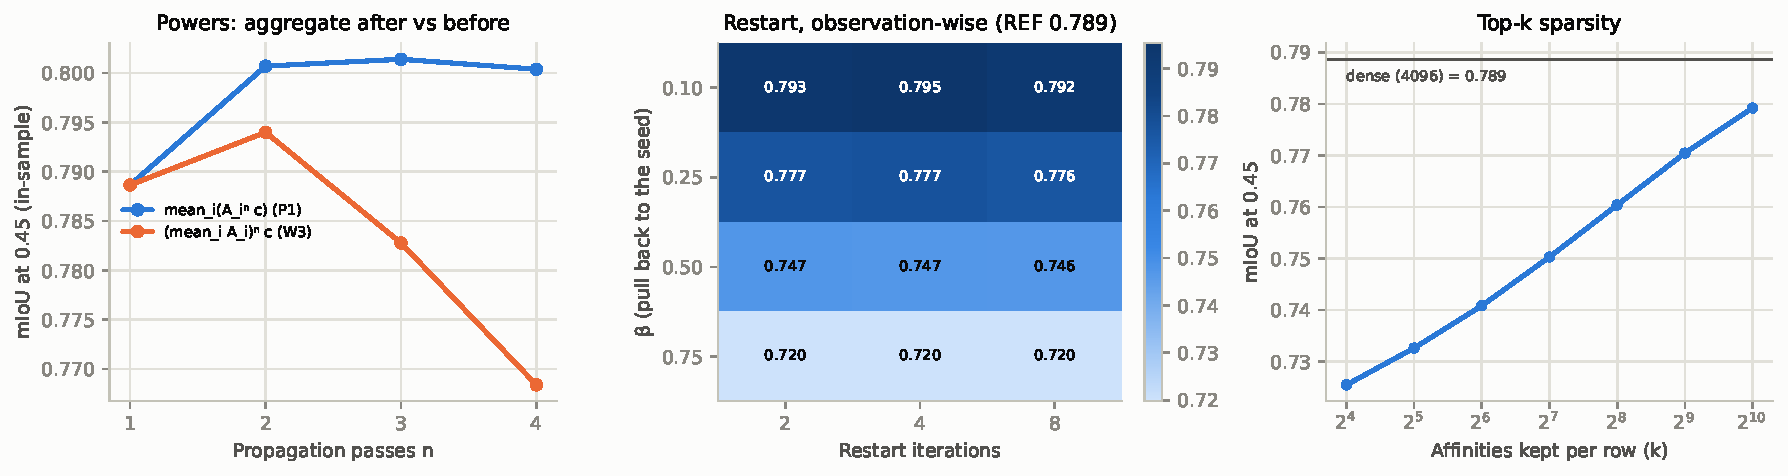
\includegraphics[width=0.8\linewidth]{evidence/figures/a8_propagation.pdf}
\caption{Propagation: passes under both aggregation orders, restart, and top-$k$ sparsity (in-sample).}\label{fig:rec_a8_propagation}
\end{figure}
\begin{figure}[H]\centering
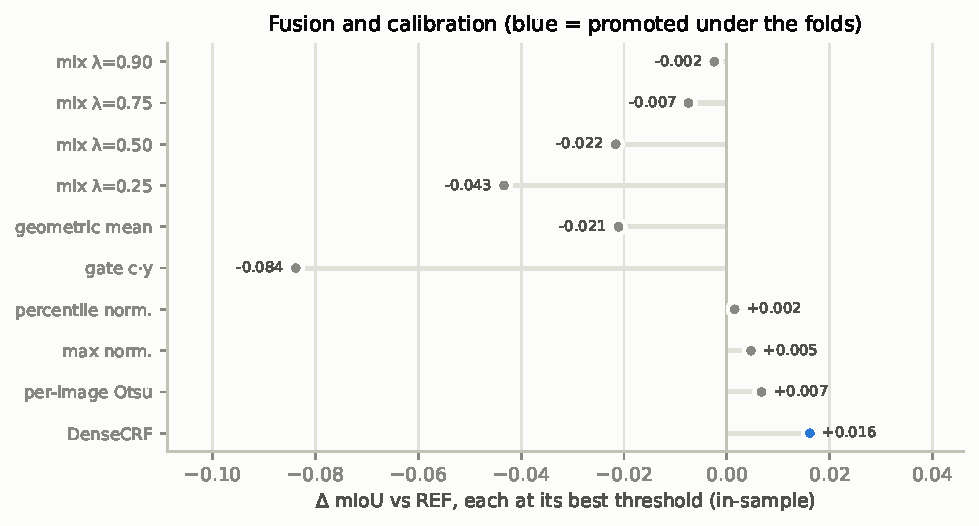
\includegraphics[width=0.55\linewidth]{evidence/figures/a9_fusion.pdf}
\caption{Fusion and calibration: change against REF, each at its best threshold (in-sample).}\label{fig:rec_a9_fusion}
\end{figure}
\begin{figure}[H]\centering
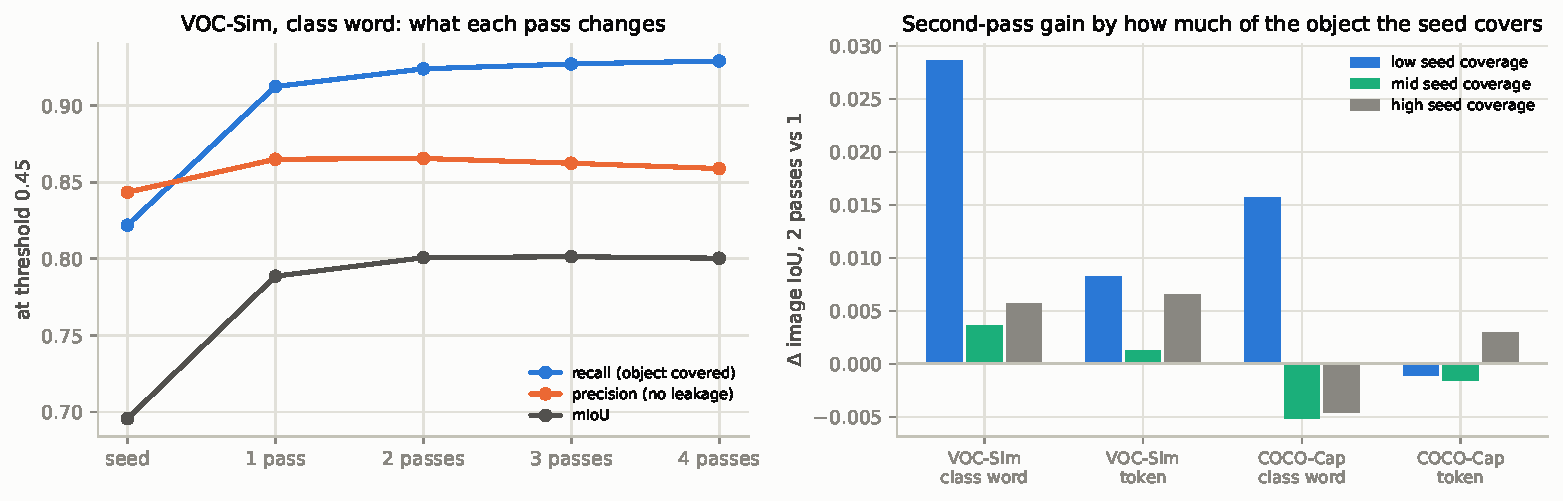
\includegraphics[width=0.8\linewidth]{evidence/figures/an1_propagation_depth.pdf}
\caption{AN1: what each pass changes, and the second-pass gain by seed coverage.}\label{fig:rec_an1_propagation_depth}
\end{figure}
\begin{figure}[H]\centering
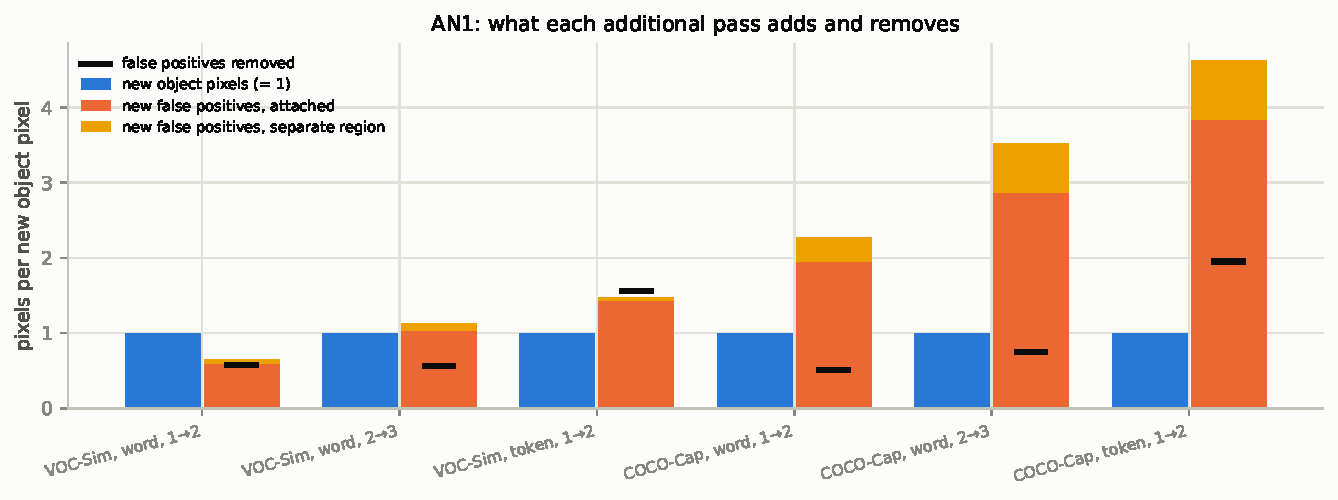
\includegraphics[width=0.8\linewidth]{evidence/figures/an1_spatial.pdf}
\caption{AN1 part 2: new object pixels, new false positives (attached or separate) and removed false positives, per new object pixel.}\label{fig:rec_an1_spatial}
\end{figure}
\begin{figure}[H]\centering
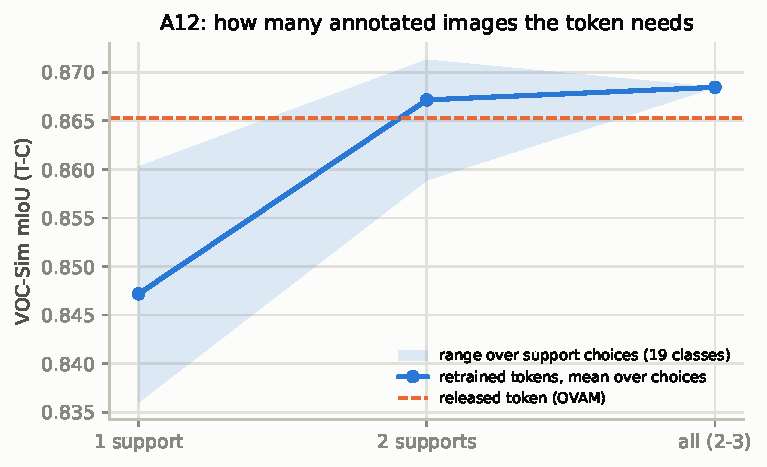
\includegraphics[width=0.45\linewidth]{evidence/figures/a12_shots.pdf}
\caption{A12: VOC-Sim mIoU against the number of annotated support images per class (T-C pipeline).}\label{fig:rec_a12_shots}
\end{figure}

\subsection{Every cell of every later package}
\label{sec:supp_record_cells}
Each package below is described in its own registration and result sections of the protocol (Sec.\ numbers in the headings). For every cell the tables give its best full-VOC threshold $t^*$, VOC-Sim mIoU there (in-sample), the change against the reference of the screen that lists the cell, a threshold-only OOF mIoU ($t^*$ chosen on four folds, scored on the fifth; the cell itself is fixed, so this is not the OOF of a selection), and COCO-Cap mIoU at the VOC $t^*$. Small differences from the paper's tables come from the one-pass reference being recomputed in each run (0.7873--0.7875 OOF across environments).

% Generated by scripts/paper/supp_experiment_record.py; do not edit.
\subsubsection{Cross-attention seed}
\paragraph{A3: A3 (Sec.~27).}
{\scriptsize\setlength{\tabcolsep}{4pt}
\begin{longtable}{@{}>{\raggedright\arraybackslash}p{5.2cm}rrrr@{}}
\caption{\textbf{A3: every cell} (6 cells). Screen references (\texttt{C/reference}) in bold; promoted cell marked $\star$. $\Delta$ in mIoU points against the reference of the screen that lists the cell.}\label{tab:record_caconfirmation}\\
\toprule
Cell & $t^*$ & VOC & $\Delta$ & OOF \\
\midrule
\endfirsthead
\toprule
Cell & $t^*$ & VOC & $\Delta$ & OOF \\
\midrule
\endhead
\midrule\multicolumn{5}{r}{\emph{continued}}\\
\endfoot
\bottomrule
\endlastfoot
\textbf{\texttt{C/\allowbreak{}reference}} & 0.350 & 0.7057 & +0.00 & 0.7057 \\
\texttt{C/\allowbreak{}R}$^\star$ & 0.350 & 0.7067 & +0.10 & 0.7067 \\
\texttt{C/\allowbreak{}L} & 0.350 & 0.7035 & -0.22 & 0.7035 \\
\texttt{C/\allowbreak{}H} & 0.350 & 0.7056 & -0.01 & 0.7056 \\
\texttt{C/\allowbreak{}R+\allowbreak{}H} & 0.350 & 0.7058 & +0.01 & 0.7058 \\
\texttt{C/\allowbreak{}L+\allowbreak{}H} & 0.350 & 0.7020 & -0.37 & 0.7020 \\
\end{longtable}}

\subsubsection{Self-attention module}
\paragraph{A6: A6 (Sec.~33).}
{\scriptsize\setlength{\tabcolsep}{4pt}
\begin{longtable}{@{}>{\raggedright\arraybackslash}p{5.2cm}rrrr@{}}
\caption{\textbf{A6: every cell} (13 cells). Screen references (\texttt{C/reference}) in bold; promoted cell marked $\star$. $\Delta$ in mIoU points against the reference of the screen that lists the cell.}\label{tab:record_saconfirmation}\\
\toprule
Cell & $t^*$ & VOC & $\Delta$ & OOF \\
\midrule
\endfirsthead
\toprule
Cell & $t^*$ & VOC & $\Delta$ & OOF \\
\midrule
\endhead
\midrule\multicolumn{5}{r}{\emph{continued}}\\
\endfoot
\bottomrule
\endlastfoot
\texttt{CHECK/\allowbreak{}ca\_\allowbreak{}seed} & 0.350 & 0.7068 & -4.88 & 0.7068 \\
\textbf{\texttt{C/\allowbreak{}reference}} & 0.450 & 0.7556 & +0.00 & 0.7556 \\
\texttt{C/\allowbreak{}T} & 0.450 & 0.7710 & +1.53 & 0.7710 \\
\texttt{C/\allowbreak{}R} & 0.450 & 0.7676 & +1.19 & 0.7676 \\
\texttt{C/\allowbreak{}L}$^\star$ & 0.450 & 0.7887 & +3.30 & 0.7887 \\
\texttt{C/\allowbreak{}H} & 0.450 & 0.7613 & +0.57 & 0.7613 \\
\texttt{C/\allowbreak{}T+\allowbreak{}R} & 0.450 & 0.7749 & +1.93 & 0.7749 \\
\texttt{C/\allowbreak{}T+\allowbreak{}L} & 0.450 & 0.7820 & +2.64 & 0.7820 \\
\texttt{C/\allowbreak{}T+\allowbreak{}H} & 0.450 & 0.7732 & +1.75 & 0.7732 \\
\texttt{C/\allowbreak{}R+\allowbreak{}H} & 0.450 & 0.7656 & +0.99 & 0.7656 \\
\texttt{C/\allowbreak{}L+\allowbreak{}H} & 0.450 & 0.7871 & +3.14 & 0.7871 \\
\texttt{C/\allowbreak{}T+\allowbreak{}R+\allowbreak{}H} & 0.450 & 0.7692 & +1.36 & 0.7692 \\
\texttt{C/\allowbreak{}T+\allowbreak{}L+\allowbreak{}H} & 0.450 & 0.7825 & +2.68 & 0.7825 \\
\end{longtable}}

\paragraph{A7: A7 (Sec.~36).}
{\scriptsize\setlength{\tabcolsep}{4pt}
\begin{longtable}{@{}>{\raggedright\arraybackslash}p{5.2cm}rrrr@{}}
\caption{\textbf{A7: every cell} (78 cells). Screen references (\texttt{CA=C/R$|$SA=C/L}) in bold; promoted cell marked $\star$. $\Delta$ in mIoU points against the reference of the screen that lists the cell.}\label{tab:record_jointcasacartesian}\\
\toprule
Cell & $t^*$ & VOC & $\Delta$ & OOF \\
\midrule
\endfirsthead
\toprule
Cell & $t^*$ & VOC & $\Delta$ & OOF \\
\midrule
\endhead
\midrule\multicolumn{5}{r}{\emph{continued}}\\
\endfoot
\bottomrule
\endlastfoot
\texttt{CA=\allowbreak{}C/\allowbreak{}reference$|$SA=\allowbreak{}none} & 0.350 & 0.7059 & -8.28 & 0.7059 \\
\texttt{CA=\allowbreak{}C/\allowbreak{}reference$|$SA=\allowbreak{}C/\allowbreak{}reference} & 0.450 & 0.7444 & -4.43 & 0.7444 \\
\texttt{CA=\allowbreak{}C/\allowbreak{}reference$|$SA=\allowbreak{}C/\allowbreak{}T} & 0.450 & 0.7573 & -3.14 & 0.7573 \\
\texttt{CA=\allowbreak{}C/\allowbreak{}reference$|$SA=\allowbreak{}C/\allowbreak{}R} & 0.450 & 0.7521 & -3.65 & 0.7521 \\
\texttt{CA=\allowbreak{}C/\allowbreak{}reference$|$SA=\allowbreak{}C/\allowbreak{}L} & 0.450 & 0.7705 & -1.81 & 0.7705 \\
\texttt{CA=\allowbreak{}C/\allowbreak{}reference$|$SA=\allowbreak{}C/\allowbreak{}H} & 0.450 & 0.7495 & -3.91 & 0.7495 \\
\texttt{CA=\allowbreak{}C/\allowbreak{}reference$|$SA=\allowbreak{}C/\allowbreak{}T+\allowbreak{}R} & 0.350 & 0.7580 & -3.07 & 0.7497 \\
\texttt{CA=\allowbreak{}C/\allowbreak{}reference$|$SA=\allowbreak{}C/\allowbreak{}T+\allowbreak{}L} & 0.450 & 0.7616 & -2.71 & 0.7546 \\
\texttt{CA=\allowbreak{}C/\allowbreak{}reference$|$SA=\allowbreak{}C/\allowbreak{}T+\allowbreak{}H} & 0.450 & 0.7582 & -3.05 & 0.7582 \\
\texttt{CA=\allowbreak{}C/\allowbreak{}reference$|$SA=\allowbreak{}C/\allowbreak{}R+\allowbreak{}H} & 0.450 & 0.7496 & -3.91 & 0.7496 \\
\texttt{CA=\allowbreak{}C/\allowbreak{}reference$|$SA=\allowbreak{}C/\allowbreak{}L+\allowbreak{}H} & 0.450 & 0.7688 & -1.98 & 0.7688 \\
\texttt{CA=\allowbreak{}C/\allowbreak{}reference$|$SA=\allowbreak{}C/\allowbreak{}T+\allowbreak{}R+\allowbreak{}H} & 0.350 & 0.7581 & -3.05 & 0.7581 \\
\texttt{CA=\allowbreak{}C/\allowbreak{}reference$|$SA=\allowbreak{}C/\allowbreak{}T+\allowbreak{}L+\allowbreak{}H} & 0.450 & 0.7621 & -2.66 & 0.7567 \\
\texttt{CA=\allowbreak{}C/\allowbreak{}R$|$SA=\allowbreak{}none} & 0.350 & 0.7068 & -8.18 & 0.7068 \\
\texttt{CA=\allowbreak{}C/\allowbreak{}R$|$SA=\allowbreak{}C/\allowbreak{}reference} & 0.450 & 0.7556 & -3.30 & 0.7556 \\
\texttt{CA=\allowbreak{}C/\allowbreak{}R$|$SA=\allowbreak{}C/\allowbreak{}T} & 0.450 & 0.7710 & -1.77 & 0.7710 \\
\texttt{CA=\allowbreak{}C/\allowbreak{}R$|$SA=\allowbreak{}C/\allowbreak{}R} & 0.450 & 0.7676 & -2.11 & 0.7676 \\
\textbf{\texttt{CA=\allowbreak{}C/\allowbreak{}R$|$SA=\allowbreak{}C/\allowbreak{}L}} & 0.450 & 0.7887 & +0.00 & 0.7887 \\
\texttt{CA=\allowbreak{}C/\allowbreak{}R$|$SA=\allowbreak{}C/\allowbreak{}H} & 0.450 & 0.7613 & -2.74 & 0.7613 \\
\texttt{CA=\allowbreak{}C/\allowbreak{}R$|$SA=\allowbreak{}C/\allowbreak{}T+\allowbreak{}R} & 0.450 & 0.7749 & -1.38 & 0.7749 \\
\texttt{CA=\allowbreak{}C/\allowbreak{}R$|$SA=\allowbreak{}C/\allowbreak{}T+\allowbreak{}L} & 0.450 & 0.7820 & -0.66 & 0.7820 \\
\texttt{CA=\allowbreak{}C/\allowbreak{}R$|$SA=\allowbreak{}C/\allowbreak{}T+\allowbreak{}H} & 0.450 & 0.7732 & -1.55 & 0.7732 \\
\texttt{CA=\allowbreak{}C/\allowbreak{}R$|$SA=\allowbreak{}C/\allowbreak{}R+\allowbreak{}H} & 0.450 & 0.7656 & -2.31 & 0.7656 \\
\texttt{CA=\allowbreak{}C/\allowbreak{}R$|$SA=\allowbreak{}C/\allowbreak{}L+\allowbreak{}H} & 0.450 & 0.7871 & -0.16 & 0.7871 \\
\texttt{CA=\allowbreak{}C/\allowbreak{}R$|$SA=\allowbreak{}C/\allowbreak{}T+\allowbreak{}R+\allowbreak{}H} & 0.450 & 0.7692 & -1.94 & 0.7692 \\
\texttt{CA=\allowbreak{}C/\allowbreak{}R$|$SA=\allowbreak{}C/\allowbreak{}T+\allowbreak{}L+\allowbreak{}H} & 0.450 & 0.7825 & -0.62 & 0.7825 \\
\texttt{CA=\allowbreak{}C/\allowbreak{}L$|$SA=\allowbreak{}none} & 0.350 & 0.7037 & -8.49 & 0.7037 \\
\texttt{CA=\allowbreak{}C/\allowbreak{}L$|$SA=\allowbreak{}C/\allowbreak{}reference} & 0.450 & 0.7473 & -4.14 & 0.7473 \\
\texttt{CA=\allowbreak{}C/\allowbreak{}L$|$SA=\allowbreak{}C/\allowbreak{}T} & 0.450 & 0.7622 & -2.65 & 0.7622 \\
\texttt{CA=\allowbreak{}C/\allowbreak{}L$|$SA=\allowbreak{}C/\allowbreak{}R} & 0.450 & 0.7571 & -3.15 & 0.7571 \\
\texttt{CA=\allowbreak{}C/\allowbreak{}L$|$SA=\allowbreak{}C/\allowbreak{}L} & 0.450 & 0.7773 & -1.13 & 0.7773 \\
\texttt{CA=\allowbreak{}C/\allowbreak{}L$|$SA=\allowbreak{}C/\allowbreak{}H} & 0.450 & 0.7529 & -3.57 & 0.7529 \\
\texttt{CA=\allowbreak{}C/\allowbreak{}L$|$SA=\allowbreak{}C/\allowbreak{}T+\allowbreak{}R} & 0.450 & 0.7650 & -2.36 & 0.7650 \\
\texttt{CA=\allowbreak{}C/\allowbreak{}L$|$SA=\allowbreak{}C/\allowbreak{}T+\allowbreak{}L} & 0.450 & 0.7714 & -1.73 & 0.7714 \\
\texttt{CA=\allowbreak{}C/\allowbreak{}L$|$SA=\allowbreak{}C/\allowbreak{}T+\allowbreak{}H} & 0.450 & 0.7651 & -2.36 & 0.7651 \\
\texttt{CA=\allowbreak{}C/\allowbreak{}L$|$SA=\allowbreak{}C/\allowbreak{}R+\allowbreak{}H} & 0.450 & 0.7552 & -3.34 & 0.7552 \\
\texttt{CA=\allowbreak{}C/\allowbreak{}L$|$SA=\allowbreak{}C/\allowbreak{}L+\allowbreak{}H} & 0.450 & 0.7760 & -1.27 & 0.7760 \\
\texttt{CA=\allowbreak{}C/\allowbreak{}L$|$SA=\allowbreak{}C/\allowbreak{}T+\allowbreak{}R+\allowbreak{}H} & 0.450 & 0.7603 & -2.84 & 0.7564 \\
\texttt{CA=\allowbreak{}C/\allowbreak{}L$|$SA=\allowbreak{}C/\allowbreak{}T+\allowbreak{}L+\allowbreak{}H} & 0.450 & 0.7720 & -1.67 & 0.7720 \\
\texttt{CA=\allowbreak{}C/\allowbreak{}H$|$SA=\allowbreak{}none} & 0.350 & 0.7057 & -8.30 & 0.7057 \\
\texttt{CA=\allowbreak{}C/\allowbreak{}H$|$SA=\allowbreak{}C/\allowbreak{}reference} & 0.450 & 0.7465 & -4.22 & 0.7465 \\
\texttt{CA=\allowbreak{}C/\allowbreak{}H$|$SA=\allowbreak{}C/\allowbreak{}T} & 0.450 & 0.7606 & -2.81 & 0.7606 \\
\texttt{CA=\allowbreak{}C/\allowbreak{}H$|$SA=\allowbreak{}C/\allowbreak{}R} & 0.450 & 0.7551 & -3.35 & 0.7551 \\
\texttt{CA=\allowbreak{}C/\allowbreak{}H$|$SA=\allowbreak{}C/\allowbreak{}L} & 0.450 & 0.7738 & -1.48 & 0.7738 \\
\texttt{CA=\allowbreak{}C/\allowbreak{}H$|$SA=\allowbreak{}C/\allowbreak{}H} & 0.450 & 0.7519 & -3.67 & 0.7519 \\
\texttt{CA=\allowbreak{}C/\allowbreak{}H$|$SA=\allowbreak{}C/\allowbreak{}T+\allowbreak{}R} & 0.450 & 0.7612 & -2.75 & 0.7564 \\
\texttt{CA=\allowbreak{}C/\allowbreak{}H$|$SA=\allowbreak{}C/\allowbreak{}T+\allowbreak{}L} & 0.450 & 0.7670 & -2.17 & 0.7670 \\
\texttt{CA=\allowbreak{}C/\allowbreak{}H$|$SA=\allowbreak{}C/\allowbreak{}T+\allowbreak{}H} & 0.450 & 0.7624 & -2.63 & 0.7624 \\
\texttt{CA=\allowbreak{}C/\allowbreak{}H$|$SA=\allowbreak{}C/\allowbreak{}R+\allowbreak{}H} & 0.450 & 0.7528 & -3.59 & 0.7528 \\
\texttt{CA=\allowbreak{}C/\allowbreak{}H$|$SA=\allowbreak{}C/\allowbreak{}L+\allowbreak{}H} & 0.450 & 0.7722 & -1.64 & 0.7722 \\
\texttt{CA=\allowbreak{}C/\allowbreak{}H$|$SA=\allowbreak{}C/\allowbreak{}T+\allowbreak{}R+\allowbreak{}H} & 0.350 & 0.7588 & -2.99 & 0.7588 \\
\texttt{CA=\allowbreak{}C/\allowbreak{}H$|$SA=\allowbreak{}C/\allowbreak{}T+\allowbreak{}L+\allowbreak{}H} & 0.450 & 0.7674 & -2.13 & 0.7674 \\
\texttt{CA=\allowbreak{}C/\allowbreak{}R+\allowbreak{}H$|$SA=\allowbreak{}none} & 0.350 & 0.7059 & -8.28 & 0.7059 \\
\texttt{CA=\allowbreak{}C/\allowbreak{}R+\allowbreak{}H$|$SA=\allowbreak{}C/\allowbreak{}reference} & 0.450 & 0.7568 & -3.19 & 0.7568 \\
\texttt{CA=\allowbreak{}C/\allowbreak{}R+\allowbreak{}H$|$SA=\allowbreak{}C/\allowbreak{}T} & 0.450 & 0.7723 & -1.63 & 0.7723 \\
\texttt{CA=\allowbreak{}C/\allowbreak{}R+\allowbreak{}H$|$SA=\allowbreak{}C/\allowbreak{}R} & 0.450 & 0.7691 & -1.96 & 0.7691 \\
\texttt{CA=\allowbreak{}C/\allowbreak{}R+\allowbreak{}H$|$SA=\allowbreak{}C/\allowbreak{}L} & 0.450 & 0.7904 & +0.17 & 0.7904 \\
\texttt{CA=\allowbreak{}C/\allowbreak{}R+\allowbreak{}H$|$SA=\allowbreak{}C/\allowbreak{}H} & 0.450 & 0.7623 & -2.63 & 0.7623 \\
\texttt{CA=\allowbreak{}C/\allowbreak{}R+\allowbreak{}H$|$SA=\allowbreak{}C/\allowbreak{}T+\allowbreak{}R} & 0.450 & 0.7765 & -1.22 & 0.7765 \\
\texttt{CA=\allowbreak{}C/\allowbreak{}R+\allowbreak{}H$|$SA=\allowbreak{}C/\allowbreak{}T+\allowbreak{}L} & 0.450 & 0.7826 & -0.60 & 0.7826 \\
\texttt{CA=\allowbreak{}C/\allowbreak{}R+\allowbreak{}H$|$SA=\allowbreak{}C/\allowbreak{}T+\allowbreak{}H} & 0.450 & 0.7748 & -1.39 & 0.7748 \\
\texttt{CA=\allowbreak{}C/\allowbreak{}R+\allowbreak{}H$|$SA=\allowbreak{}C/\allowbreak{}R+\allowbreak{}H} & 0.450 & 0.7671 & -2.16 & 0.7671 \\
\texttt{CA=\allowbreak{}C/\allowbreak{}R+\allowbreak{}H$|$SA=\allowbreak{}C/\allowbreak{}L+\allowbreak{}H} & 0.450 & 0.7888 & +0.01 & 0.7888 \\
\texttt{CA=\allowbreak{}C/\allowbreak{}R+\allowbreak{}H$|$SA=\allowbreak{}C/\allowbreak{}T+\allowbreak{}R+\allowbreak{}H} & 0.450 & 0.7711 & -1.76 & 0.7711 \\
\texttt{CA=\allowbreak{}C/\allowbreak{}R+\allowbreak{}H$|$SA=\allowbreak{}C/\allowbreak{}T+\allowbreak{}L+\allowbreak{}H} & 0.450 & 0.7831 & -0.55 & 0.7831 \\
\texttt{CA=\allowbreak{}C/\allowbreak{}L+\allowbreak{}H$|$SA=\allowbreak{}none} & 0.350 & 0.7023 & -8.64 & 0.7023 \\
\texttt{CA=\allowbreak{}C/\allowbreak{}L+\allowbreak{}H$|$SA=\allowbreak{}C/\allowbreak{}reference} & 0.450 & 0.7475 & -4.11 & 0.7475 \\
\texttt{CA=\allowbreak{}C/\allowbreak{}L+\allowbreak{}H$|$SA=\allowbreak{}C/\allowbreak{}T} & 0.450 & 0.7632 & -2.54 & 0.7632 \\
\texttt{CA=\allowbreak{}C/\allowbreak{}L+\allowbreak{}H$|$SA=\allowbreak{}C/\allowbreak{}R} & 0.450 & 0.7576 & -3.11 & 0.7576 \\
\texttt{CA=\allowbreak{}C/\allowbreak{}L+\allowbreak{}H$|$SA=\allowbreak{}C/\allowbreak{}L} & 0.450 & 0.7780 & -1.07 & 0.7780 \\
\texttt{CA=\allowbreak{}C/\allowbreak{}L+\allowbreak{}H$|$SA=\allowbreak{}C/\allowbreak{}H} & 0.450 & 0.7533 & -3.54 & 0.7533 \\
\texttt{CA=\allowbreak{}C/\allowbreak{}L+\allowbreak{}H$|$SA=\allowbreak{}C/\allowbreak{}T+\allowbreak{}R} & 0.450 & 0.7670 & -2.17 & 0.7670 \\
\texttt{CA=\allowbreak{}C/\allowbreak{}L+\allowbreak{}H$|$SA=\allowbreak{}C/\allowbreak{}T+\allowbreak{}L} & 0.450 & 0.7730 & -1.57 & 0.7730 \\
\texttt{CA=\allowbreak{}C/\allowbreak{}L+\allowbreak{}H$|$SA=\allowbreak{}C/\allowbreak{}T+\allowbreak{}H} & 0.450 & 0.7666 & -2.21 & 0.7666 \\
\texttt{CA=\allowbreak{}C/\allowbreak{}L+\allowbreak{}H$|$SA=\allowbreak{}C/\allowbreak{}R+\allowbreak{}H} & 0.450 & 0.7558 & -3.29 & 0.7558 \\
\texttt{CA=\allowbreak{}C/\allowbreak{}L+\allowbreak{}H$|$SA=\allowbreak{}C/\allowbreak{}L+\allowbreak{}H} & 0.450 & 0.7765 & -1.22 & 0.7765 \\
\texttt{CA=\allowbreak{}C/\allowbreak{}L+\allowbreak{}H$|$SA=\allowbreak{}C/\allowbreak{}T+\allowbreak{}R+\allowbreak{}H} & 0.450 & 0.7631 & -2.55 & 0.7631 \\
\texttt{CA=\allowbreak{}C/\allowbreak{}L+\allowbreak{}H$|$SA=\allowbreak{}C/\allowbreak{}T+\allowbreak{}L+\allowbreak{}H} & 0.450 & 0.7733 & -1.54 & 0.7733 \\
\end{longtable}}

\subsubsection{Propagation, refinement and tokens}
\paragraph{A8: A8 (Sec.~43).}
{\scriptsize\setlength{\tabcolsep}{4pt}
\begin{longtable}{@{}>{\raggedright\arraybackslash}p{5.2cm}rrrr@{}}
\caption{\textbf{A8: every cell} (40 cells). Screen references (\texttt{REF/one\_pass}) in bold; promoted cell marked $\star$. $\Delta$ in mIoU points against the reference of the screen that lists the cell.}\label{tab:record_propagationpackage}\\
\toprule
Cell & $t^*$ & VOC & $\Delta$ & OOF \\
\midrule
\endfirsthead
\toprule
Cell & $t^*$ & VOC & $\Delta$ & OOF \\
\midrule
\endhead
\midrule\multicolumn{5}{r}{\emph{continued}}\\
\endfoot
\bottomrule
\endlastfoot
\texttt{CHECK/\allowbreak{}ca\_\allowbreak{}seed} & 0.400 & 0.7136 & -7.52 & 0.7130 \\
\textbf{\texttt{REF/\allowbreak{}one\_\allowbreak{}pass}} & 0.425 & 0.7888 & +0.00 & 0.7875 \\
\texttt{P1/\allowbreak{}obs\_\allowbreak{}n2}$^\star$ & 0.450 & 0.8007 & +1.19 & 0.7998 \\
\texttt{P1/\allowbreak{}obs\_\allowbreak{}n3} & 0.475 & 0.8019 & +1.31 & 0.8004 \\
\texttt{P1/\allowbreak{}obs\_\allowbreak{}n4} & 0.475 & 0.8005 & +1.17 & 0.7992 \\
\texttt{W3/\allowbreak{}mean\_\allowbreak{}n1} & 0.425 & 0.7888 & +0.00 & 0.7875 \\
\texttt{W3/\allowbreak{}mean\_\allowbreak{}n2} & 0.475 & 0.7950 & +0.62 & 0.7950 \\
\texttt{W3/\allowbreak{}mean\_\allowbreak{}n3} & 0.475 & 0.7857 & -0.31 & 0.7841 \\
\texttt{W3/\allowbreak{}mean\_\allowbreak{}n4} & 0.475 & 0.7706 & -1.82 & 0.7706 \\
\texttt{P2/\allowbreak{}obs\_\allowbreak{}b10\_\allowbreak{}n2} & 0.450 & 0.7934 & +0.46 & 0.7922 \\
\texttt{P2/\allowbreak{}obs\_\allowbreak{}b10\_\allowbreak{}n4} & 0.450 & 0.7954 & +0.66 & 0.7954 \\
\texttt{P2/\allowbreak{}obs\_\allowbreak{}b10\_\allowbreak{}n8} & 0.450 & 0.7922 & +0.34 & 0.7922 \\
\texttt{P2/\allowbreak{}obs\_\allowbreak{}b25\_\allowbreak{}n2} & 0.425 & 0.7788 & -1.00 & 0.7788 \\
\texttt{P2/\allowbreak{}obs\_\allowbreak{}b25\_\allowbreak{}n4} & 0.425 & 0.7791 & -0.97 & 0.7791 \\
\texttt{P2/\allowbreak{}obs\_\allowbreak{}b25\_\allowbreak{}n8} & 0.425 & 0.7775 & -1.12 & 0.7775 \\
\texttt{P2/\allowbreak{}obs\_\allowbreak{}b50\_\allowbreak{}n2} & 0.400 & 0.7536 & -3.52 & 0.7536 \\
\texttt{P2/\allowbreak{}obs\_\allowbreak{}b50\_\allowbreak{}n4} & 0.400 & 0.7532 & -3.56 & 0.7524 \\
\texttt{P2/\allowbreak{}obs\_\allowbreak{}b50\_\allowbreak{}n8} & 0.400 & 0.7530 & -3.58 & 0.7522 \\
\texttt{P2/\allowbreak{}obs\_\allowbreak{}b75\_\allowbreak{}n2} & 0.400 & 0.7321 & -5.67 & 0.7321 \\
\texttt{P2/\allowbreak{}obs\_\allowbreak{}b75\_\allowbreak{}n4} & 0.400 & 0.7320 & -5.67 & 0.7320 \\
\texttt{P2/\allowbreak{}obs\_\allowbreak{}b75\_\allowbreak{}n8} & 0.400 & 0.7320 & -5.68 & 0.7320 \\
\texttt{P2/\allowbreak{}mean\_\allowbreak{}b10\_\allowbreak{}n2} & 0.450 & 0.7888 & -0.00 & 0.7888 \\
\texttt{P2/\allowbreak{}mean\_\allowbreak{}b10\_\allowbreak{}n4} & 0.450 & 0.7825 & -0.63 & 0.7814 \\
\texttt{P2/\allowbreak{}mean\_\allowbreak{}b10\_\allowbreak{}n8} & 0.450 & 0.7763 & -1.25 & 0.7763 \\
\texttt{P2/\allowbreak{}mean\_\allowbreak{}b25\_\allowbreak{}n2} & 0.425 & 0.7752 & -1.36 & 0.7752 \\
\texttt{P2/\allowbreak{}mean\_\allowbreak{}b25\_\allowbreak{}n4} & 0.425 & 0.7706 & -1.81 & 0.7706 \\
\texttt{P2/\allowbreak{}mean\_\allowbreak{}b25\_\allowbreak{}n8} & 0.425 & 0.7676 & -2.12 & 0.7676 \\
\texttt{P2/\allowbreak{}mean\_\allowbreak{}b50\_\allowbreak{}n2} & 0.400 & 0.7515 & -3.73 & 0.7508 \\
\texttt{P2/\allowbreak{}mean\_\allowbreak{}b50\_\allowbreak{}n4} & 0.400 & 0.7498 & -3.90 & 0.7490 \\
\texttt{P2/\allowbreak{}mean\_\allowbreak{}b50\_\allowbreak{}n8} & 0.400 & 0.7495 & -3.93 & 0.7486 \\
\texttt{P2/\allowbreak{}mean\_\allowbreak{}b75\_\allowbreak{}n2} & 0.400 & 0.7316 & -5.72 & 0.7316 \\
\texttt{P2/\allowbreak{}mean\_\allowbreak{}b75\_\allowbreak{}n4} & 0.400 & 0.7313 & -5.75 & 0.7313 \\
\texttt{P2/\allowbreak{}mean\_\allowbreak{}b75\_\allowbreak{}n8} & 0.400 & 0.7313 & -5.75 & 0.7313 \\
\texttt{P6/\allowbreak{}topk\_\allowbreak{}0016} & 0.425 & 0.7270 & -6.18 & 0.7270 \\
\texttt{P6/\allowbreak{}topk\_\allowbreak{}0032} & 0.425 & 0.7335 & -5.53 & 0.7335 \\
\texttt{P6/\allowbreak{}topk\_\allowbreak{}0064} & 0.425 & 0.7409 & -4.79 & 0.7402 \\
\texttt{P6/\allowbreak{}topk\_\allowbreak{}0128} & 0.450 & 0.7503 & -3.85 & 0.7503 \\
\texttt{P6/\allowbreak{}topk\_\allowbreak{}0256} & 0.450 & 0.7604 & -2.84 & 0.7604 \\
\texttt{P6/\allowbreak{}topk\_\allowbreak{}0512} & 0.450 & 0.7704 & -1.83 & 0.7704 \\
\texttt{P6/\allowbreak{}topk\_\allowbreak{}1024} & 0.450 & 0.7792 & -0.96 & 0.7792 \\
\end{longtable}}

\paragraph{A9: A9 (Sec.~44).}
{\scriptsize\setlength{\tabcolsep}{4pt}
\begin{longtable}{@{}>{\raggedright\arraybackslash}p{5.2cm}rrrr@{}}
\caption{\textbf{A9: every cell} (12 cells). Screen references (\texttt{REF/one\_pass}) in bold; promoted cell marked $\star$. $\Delta$ in mIoU points against the reference of the screen that lists the cell.}\label{tab:record_fusioncalibration}\\
\toprule
Cell & $t^*$ & VOC & $\Delta$ & OOF \\
\midrule
\endfirsthead
\toprule
Cell & $t^*$ & VOC & $\Delta$ & OOF \\
\midrule
\endhead
\midrule\multicolumn{5}{r}{\emph{continued}}\\
\endfoot
\bottomrule
\endlastfoot
\texttt{CHECK/\allowbreak{}ca\_\allowbreak{}seed} & 0.400 & 0.7134 & -7.54 & 0.7127 \\
\textbf{\texttt{REF/\allowbreak{}one\_\allowbreak{}pass}} & 0.425 & 0.7888 & +0.00 & 0.7875 \\
\texttt{P4/\allowbreak{}lam25} & 0.400 & 0.7454 & -4.33 & 0.7454 \\
\texttt{P4/\allowbreak{}lam50} & 0.425 & 0.7671 & -2.16 & 0.7659 \\
\texttt{P4/\allowbreak{}lam75} & 0.425 & 0.7813 & -0.74 & 0.7813 \\
\texttt{P4/\allowbreak{}lam90} & 0.425 & 0.7863 & -0.24 & 0.7851 \\
\texttt{F3/\allowbreak{}gate} & 0.300 & 0.7049 & -8.38 & 0.7049 \\
\texttt{F4/\allowbreak{}geomean} & 0.425 & 0.7677 & -2.11 & 0.7664 \\
\texttt{N2/\allowbreak{}percentile} & 0.475 & 0.7903 & +0.15 & 0.7890 \\
\texttt{N3/\allowbreak{}max} & 0.600 & 0.7935 & +0.47 & 0.7935 \\
\texttt{N4/\allowbreak{}otsu} & 0.450 & 0.7955 & +0.68 & 0.7955 \\
\texttt{R2/\allowbreak{}crf}$^\star$ & 0.425 & 0.8049 & +1.61 & 0.8049 \\
\end{longtable}}

\paragraph{P3-C: P3-C (Sec.~51).}
{\scriptsize\setlength{\tabcolsep}{4pt}
\begin{longtable}{@{}>{\raggedright\arraybackslash}p{5.2cm}rrrr@{}}
\caption{\textbf{P3-C: every cell} (30 cells). Screen references (\texttt{REF/one\_pass$|$N0/global$|$R0/none}) in bold; promoted cell marked $\star$. $\Delta$ in mIoU points against the reference of the screen that lists the cell.}\label{tab:record_phase3confirmation}\\
\toprule
Cell & $t^*$ & VOC & $\Delta$ & OOF \\
\midrule
\endfirsthead
\toprule
Cell & $t^*$ & VOC & $\Delta$ & OOF \\
\midrule
\endhead
\midrule\multicolumn{5}{r}{\emph{continued}}\\
\endfoot
\bottomrule
\endlastfoot
\textbf{\texttt{REF/\allowbreak{}one\_\allowbreak{}pass$|$N0/\allowbreak{}global$|$R0/\allowbreak{}none}} & 0.425 & 0.7888 & +0.00 & 0.7875 \\
\texttt{REF/\allowbreak{}one\_\allowbreak{}pass$|$N0/\allowbreak{}global$|$R2/\allowbreak{}crf} & 0.425 & 0.8050 & +1.62 & 0.8050 \\
\texttt{REF/\allowbreak{}one\_\allowbreak{}pass$|$N2/\allowbreak{}percentile$|$R0/\allowbreak{}none} & 0.450 & 0.7903 & +0.15 & 0.7890 \\
\texttt{REF/\allowbreak{}one\_\allowbreak{}pass$|$N2/\allowbreak{}percentile$|$R2/\allowbreak{}crf} & 0.450 & 0.8066 & +1.78 & 0.8056 \\
\texttt{REF/\allowbreak{}one\_\allowbreak{}pass$|$N4/\allowbreak{}otsu$|$R0/\allowbreak{}none} & 0.450 & 0.7955 & +0.67 & 0.7955 \\
\texttt{REF/\allowbreak{}one\_\allowbreak{}pass$|$N4/\allowbreak{}otsu$|$R2/\allowbreak{}crf} & 0.450 & 0.8131 & +2.43 & 0.8131 \\
\texttt{P1/\allowbreak{}obs\_\allowbreak{}n2$|$N0/\allowbreak{}global$|$R0/\allowbreak{}none} & 0.450 & 0.8007 & +1.19 & 0.7998 \\
\texttt{P1/\allowbreak{}obs\_\allowbreak{}n2$|$N0/\allowbreak{}global$|$R2/\allowbreak{}crf}$^\star$ & 0.450 & 0.8135 & +2.47 & 0.8135 \\
\texttt{P1/\allowbreak{}obs\_\allowbreak{}n2$|$N2/\allowbreak{}percentile$|$R0/\allowbreak{}none} & 0.475 & 0.8019 & +1.31 & 0.8006 \\
\texttt{P1/\allowbreak{}obs\_\allowbreak{}n2$|$N2/\allowbreak{}percentile$|$R2/\allowbreak{}crf} & 0.450 & 0.8156 & +2.68 & 0.8143 \\
\texttt{P1/\allowbreak{}obs\_\allowbreak{}n2$|$N4/\allowbreak{}otsu$|$R0/\allowbreak{}none} & 0.450 & 0.8051 & +1.63 & 0.8051 \\
\texttt{P1/\allowbreak{}obs\_\allowbreak{}n2$|$N4/\allowbreak{}otsu$|$R2/\allowbreak{}crf}$^\star$ & 0.450 & 0.8207 & +3.19 & 0.8207 \\
\texttt{P1/\allowbreak{}obs\_\allowbreak{}n3$|$N0/\allowbreak{}global$|$R0/\allowbreak{}none} & 0.475 & 0.8019 & +1.31 & 0.8004 \\
\texttt{P1/\allowbreak{}obs\_\allowbreak{}n3$|$N0/\allowbreak{}global$|$R2/\allowbreak{}crf} & 0.450 & 0.8136 & +2.48 & 0.8125 \\
\texttt{P1/\allowbreak{}obs\_\allowbreak{}n3$|$N2/\allowbreak{}percentile$|$R0/\allowbreak{}none} & 0.475 & 0.8038 & +1.51 & 0.8022 \\
\texttt{P1/\allowbreak{}obs\_\allowbreak{}n3$|$N2/\allowbreak{}percentile$|$R2/\allowbreak{}crf} & 0.450 & 0.8167 & +2.80 & 0.8153 \\
\texttt{P1/\allowbreak{}obs\_\allowbreak{}n3$|$N4/\allowbreak{}otsu$|$R0/\allowbreak{}none} & 0.450 & 0.8017 & +1.29 & 0.8017 \\
\texttt{P1/\allowbreak{}obs\_\allowbreak{}n3$|$N4/\allowbreak{}otsu$|$R2/\allowbreak{}crf} & 0.450 & 0.8168 & +2.80 & 0.8168 \\
\texttt{P2/\allowbreak{}obs\_\allowbreak{}b10\_\allowbreak{}n4$|$N0/\allowbreak{}global$|$R0/\allowbreak{}none} & 0.450 & 0.7954 & +0.66 & 0.7954 \\
\texttt{P2/\allowbreak{}obs\_\allowbreak{}b10\_\allowbreak{}n4$|$N0/\allowbreak{}global$|$R2/\allowbreak{}crf} & 0.425 & 0.8102 & +2.14 & 0.8090 \\
\texttt{P2/\allowbreak{}obs\_\allowbreak{}b10\_\allowbreak{}n4$|$N2/\allowbreak{}percentile$|$R0/\allowbreak{}none} & 0.475 & 0.7978 & +0.90 & 0.7978 \\
\texttt{P2/\allowbreak{}obs\_\allowbreak{}b10\_\allowbreak{}n4$|$N2/\allowbreak{}percentile$|$R2/\allowbreak{}crf} & 0.450 & 0.8136 & +2.49 & 0.8136 \\
\texttt{P2/\allowbreak{}obs\_\allowbreak{}b10\_\allowbreak{}n4$|$N4/\allowbreak{}otsu$|$R0/\allowbreak{}none} & 0.450 & 0.7993 & +1.05 & 0.7993 \\
\texttt{P2/\allowbreak{}obs\_\allowbreak{}b10\_\allowbreak{}n4$|$N4/\allowbreak{}otsu$|$R2/\allowbreak{}crf} & 0.450 & 0.8168 & +2.80 & 0.8168 \\
\texttt{W3/\allowbreak{}mean\_\allowbreak{}n2$|$N0/\allowbreak{}global$|$R0/\allowbreak{}none} & 0.475 & 0.7950 & +0.62 & 0.7950 \\
\texttt{W3/\allowbreak{}mean\_\allowbreak{}n2$|$N0/\allowbreak{}global$|$R2/\allowbreak{}crf} & 0.450 & 0.8064 & +1.76 & 0.8064 \\
\texttt{W3/\allowbreak{}mean\_\allowbreak{}n2$|$N2/\allowbreak{}percentile$|$R0/\allowbreak{}none} & 0.500 & 0.7957 & +0.69 & 0.7944 \\
\texttt{W3/\allowbreak{}mean\_\allowbreak{}n2$|$N2/\allowbreak{}percentile$|$R2/\allowbreak{}crf} & 0.475 & 0.8072 & +1.84 & 0.8066 \\
\texttt{W3/\allowbreak{}mean\_\allowbreak{}n2$|$N4/\allowbreak{}otsu$|$R0/\allowbreak{}none} & 0.450 & 0.7973 & +0.85 & 0.7973 \\
\texttt{W3/\allowbreak{}mean\_\allowbreak{}n2$|$N4/\allowbreak{}otsu$|$R2/\allowbreak{}crf} & 0.450 & 0.8115 & +2.27 & 0.8115 \\
\end{longtable}}

\paragraph{A11: A11 (Sec.~50).}
{\scriptsize\setlength{\tabcolsep}{4pt}
\begin{longtable}{@{}>{\raggedright\arraybackslash}p{5.2cm}rrrr@{}}
\caption{\textbf{A11: every cell} (27 cells). Screen references (\texttt{W/REF}) in bold; promoted cell marked $\star$. $\Delta$ in mIoU points against the reference of the screen that lists the cell.}\label{tab:record_tokens}\\
\toprule
Cell & $t^*$ & VOC & $\Delta$ & OOF \\
\midrule
\endfirsthead
\toprule
Cell & $t^*$ & VOC & $\Delta$ & OOF \\
\midrule
\endhead
\midrule\multicolumn{5}{r}{\emph{continued}}\\
\endfoot
\bottomrule
\endlastfoot
\texttt{W/\allowbreak{}seed} & 0.400 & 0.7134 & -7.52 & 0.7128 \\
\textbf{\texttt{W/\allowbreak{}REF}} & 0.425 & 0.7886 & +0.00 & 0.7873 \\
\texttt{W/\allowbreak{}P1} & 0.450 & 0.8006 & +1.20 & 0.7997 \\
\texttt{W/\allowbreak{}R2} & 0.425 & 0.8047 & +1.61 & 0.8047 \\
\texttt{W/\allowbreak{}P1+\allowbreak{}R2} & 0.450 & 0.8132 & +2.46 & 0.8132 \\
\texttt{TU/\allowbreak{}seed} & 0.475 & 0.7915 & +0.29 & 0.7915 \\
\texttt{TU/\allowbreak{}REF}$^\star$ & 0.475 & 0.8435 & +5.48 & 0.8428 \\
\texttt{TU/\allowbreak{}P1} & 0.475 & 0.8476 & +5.90 & 0.8462 \\
\texttt{TU/\allowbreak{}R2} & 0.475 & 0.8580 & +6.94 & 0.8580 \\
\texttt{TU/\allowbreak{}P1+\allowbreak{}R2} & 0.475 & 0.8603 & +7.17 & 0.8603 \\
\texttt{TC/\allowbreak{}seed} & 0.475 & 0.7967 & +0.81 & 0.7967 \\
\texttt{TC/\allowbreak{}REF}$^\star$ & 0.475 & 0.8507 & +6.21 & 0.8507 \\
\texttt{TC/\allowbreak{}P1} & 0.475 & 0.8543 & +6.57 & 0.8543 \\
\texttt{TC/\allowbreak{}R2} & 0.475 & 0.8652 & +7.66 & 0.8643 \\
\texttt{TC/\allowbreak{}P1+\allowbreak{}R2} & 0.475 & 0.8669 & +7.83 & 0.8654 \\
\texttt{T1U/\allowbreak{}REF} & 0.475 & 0.8233 & +3.47 & 0.8233 \\
\texttt{T1U/\allowbreak{}P1} & 0.500 & 0.8247 & +3.61 & 0.8238 \\
\texttt{T2U/\allowbreak{}REF} & 0.500 & 0.8500 & +6.14 & 0.8500 \\
\texttt{T2U/\allowbreak{}P1} & 0.500 & 0.8546 & +6.60 & 0.8546 \\
\texttt{T3U/\allowbreak{}REF} & 0.500 & 0.8385 & +4.99 & 0.8385 \\
\texttt{T3U/\allowbreak{}P1} & 0.500 & 0.8403 & +5.16 & 0.8403 \\
\texttt{T1C/\allowbreak{}REF} & 0.475 & 0.8309 & +4.23 & 0.8309 \\
\texttt{T1C/\allowbreak{}P1} & 0.500 & 0.8338 & +4.52 & 0.8334 \\
\texttt{T2C/\allowbreak{}REF} & 0.500 & 0.8536 & +6.50 & 0.8529 \\
\texttt{T2C/\allowbreak{}P1} & 0.500 & 0.8578 & +6.92 & 0.8572 \\
\texttt{T3C/\allowbreak{}REF} & 0.500 & 0.8419 & +5.33 & 0.8419 \\
\texttt{T3C/\allowbreak{}P1} & 0.500 & 0.8430 & +5.43 & 0.8430 \\
\end{longtable}}

\subsubsection{Graph, seed and observation operators}
\paragraph{SG5: SG5 contrastive cross-attention seed (Sec.~66, 70).}
Tests whether contrasting the class-word cross-attention (CA) probability against other prompt positions closes the coverage gap between the class-word seed (seed recall 0.82) and OVAM's released token (0.93) without losing precision. Only the per-head map entering the frozen CA average changes; every seed is then run through the same five fixed pipelines. Training-free for the W-variants; the token variants use OVAM's released token, frozen.

\emph{Cell names.} Each name is $<$seed$>$/$<$pipeline$>$. Seeds: W = class word, p\_T (mean softmax probability of the class word pieces over the 77 padded prompt keys; frozen convention); WS = log p\_T - log p\_SoT (contrast with the start token); WK = p\_T/(p\_T + p\_SoT) (class word in OVAM's two-key form); WN = log p\_T - log mean of p over all non-target positions; WE = log p\_T - log mean of p over $<$EoT$>$ and padding positions; WY = mean of p\_T over the class word and its fixed synonyms (same template; 8 classes have no synonym, so WY = W for them); TC = OVAM released token with keys [$<$SoT$>$, token], p\_tok (few-shot reference, T-C); TS = log p\_tok - log p\_SoT. Pipelines: seed = CA map alone, no propagation; REF = one observation-wise SA pass through module 15, mean\_i(A\_i c); P1 = two passes, mean\_i(A\_i\^{}2 c); R2 = REF followed by OVAM's fixed DenseCRF (note: here 'R2' alone means REF+DenseCRF); P1+R2 = two passes + DenseCRF (FTF for W). 8 seeds x 5 pipelines = 40 cells.

\emph{Reference.} Four separate screens: W/REF (seed effect under one pass; candidates WS/WK/WN/WE/WY at REF), W/P1+R2 = FTF (candidates the same five at P1+R2), TC/REF (candidate TS/REF) and TC/R2 = T-C few-shot pipeline (candidate TS/R2). The seed and P1 cells of non-screened pipelines are reported only.

\emph{Decision.} The reference won 5/5 folds in all four screens and nothing was frozen (OOF W/REF 0.7873, W/P1+R2 0.8134, TC/REF 0.8496, TC/R2 0.8647). The log-ratio seeds raise seed recall to 0.96-0.98 but cut precision to 0.47-0.67 (Section 70).

{\scriptsize\setlength{\tabcolsep}{4pt}
\begin{longtable}{@{}>{\raggedright\arraybackslash}p{5.2cm}rrrrrr@{}}
\caption{\textbf{SG5: every cell} (40 cells). Screen references (\texttt{TC/R2}, \texttt{TC/REF}, \texttt{W/P1+R2}, \texttt{W/REF}) in bold; promoted cell marked $\star$. $\Delta$ in mIoU points against the reference of the screen that lists the cell.}\label{tab:record_sg5contrastiveseed}\\
\toprule
Cell & $t^*$ & VOC & $\Delta$ & OOF & COCO & $\Delta$ \\
\midrule
\endfirsthead
\toprule
Cell & $t^*$ & VOC & $\Delta$ & OOF & COCO & $\Delta$ \\
\midrule
\endhead
\midrule\multicolumn{7}{r}{\emph{continued}}\\
\endfoot
\bottomrule
\endlastfoot
\texttt{W/\allowbreak{}seed} & 0.400 & 0.7133 & -7.53 & 0.7127 & 0.5629 & -5.44 \\
\textbf{\texttt{W/\allowbreak{}REF}} & 0.425 & 0.7886 & +0.00 & 0.7873 & 0.6173 & +0.00 \\
\texttt{W/\allowbreak{}P1} & 0.450 & 0.8005 & +1.19 & 0.7997 & 0.6244 & +0.71 \\
\texttt{W/\allowbreak{}R2} & 0.425 & 0.8049 & +1.63 & 0.8049 & 0.6349 & +1.76 \\
\textbf{\texttt{W/\allowbreak{}P1+\allowbreak{}R2}} & 0.450 & 0.8134 & +0.00 & 0.8134 & 0.6370 & +0.00 \\
\texttt{WS/\allowbreak{}seed} & 0.550 & 0.7002 & -8.84 & 0.7002 & 0.5408 & -7.65 \\
\texttt{WS/\allowbreak{}REF} & 0.525 & 0.7839 & -0.47 & 0.7820 & 0.5778 & -3.95 \\
\texttt{WS/\allowbreak{}P1} & 0.525 & 0.7926 & +0.40 & 0.7912 & 0.5772 & -4.00 \\
\texttt{WS/\allowbreak{}R2} & 0.525 & 0.8019 & +1.33 & 0.7983 & 0.5933 & -2.40 \\
\texttt{WS/\allowbreak{}P1+\allowbreak{}R2} & 0.500 & 0.8059 & -0.75 & 0.8028 & 0.5742 & -6.29 \\
\texttt{WK/\allowbreak{}seed} & 0.375 & 0.7090 & -7.96 & 0.7090 & 0.5514 & -6.59 \\
\texttt{WK/\allowbreak{}REF} & 0.450 & 0.7733 & -1.53 & 0.7719 & 0.6144 & -0.29 \\
\texttt{WK/\allowbreak{}P1} & 0.450 & 0.7850 & -0.37 & 0.7850 & 0.6091 & -0.82 \\
\texttt{WK/\allowbreak{}R2} & 0.425 & 0.7886 & -0.00 & 0.7869 & 0.6208 & +0.35 \\
\texttt{WK/\allowbreak{}P1+\allowbreak{}R2} & 0.425 & 0.7978 & -1.57 & 0.7956 & 0.6093 & -2.77 \\
\texttt{WN/\allowbreak{}seed} & 0.600 & 0.6999 & -8.87 & 0.6999 & 0.5461 & -7.12 \\
\texttt{WN/\allowbreak{}REF} & 0.550 & 0.7948 & +0.62 & 0.7933 & 0.5907 & -2.66 \\
\texttt{WN/\allowbreak{}P1} & 0.550 & 0.8024 & +1.37 & 0.8001 & 0.5894 & -2.79 \\
\texttt{WN/\allowbreak{}R2} & 0.550 & 0.8127 & +2.41 & 0.8127 & 0.6050 & -1.23 \\
\texttt{WN/\allowbreak{}P1+\allowbreak{}R2} & 0.525 & 0.8165 & +0.31 & 0.8165 & 0.5880 & -4.91 \\
\texttt{WE/\allowbreak{}seed} & 0.650 & 0.5930 & -19.56 & 0.5930 & 0.4582 & -15.91 \\
\texttt{WE/\allowbreak{}REF} & 0.625 & 0.7375 & -5.11 & 0.7364 & 0.5569 & -6.04 \\
\texttt{WE/\allowbreak{}P1} & 0.625 & 0.7470 & -4.16 & 0.7459 & 0.5552 & -6.21 \\
\texttt{WE/\allowbreak{}R2} & 0.600 & 0.7499 & -3.88 & 0.7491 & 0.5599 & -5.74 \\
\texttt{WE/\allowbreak{}P1+\allowbreak{}R2} & 0.600 & 0.7542 & -5.92 & 0.7527 & 0.5547 & -8.23 \\
\texttt{WY/\allowbreak{}seed} & 0.400 & 0.7111 & -7.75 & 0.7111 & 0.5589 & -5.84 \\
\texttt{WY/\allowbreak{}REF} & 0.450 & 0.7822 & -0.64 & 0.7813 & 0.6201 & +0.28 \\
\texttt{WY/\allowbreak{}P1} & 0.450 & 0.7939 & +0.53 & 0.7929 & 0.6178 & +0.05 \\
\texttt{WY/\allowbreak{}R2} & 0.425 & 0.7978 & +0.92 & 0.7978 & 0.6283 & +1.10 \\
\texttt{WY/\allowbreak{}P1+\allowbreak{}R2} & 0.425 & 0.8059 & -0.75 & 0.8053 & 0.6202 & -1.68 \\
\texttt{TC/\allowbreak{}seed} & 0.475 & 0.7960 & +0.73 & 0.7960 & 0.6380 & +2.07 \\
\textbf{\texttt{TC/\allowbreak{}REF}} & 0.475 & 0.8501 & +0.00 & 0.8496 & 0.6680 & +0.00 \\
\texttt{TC/\allowbreak{}P1} & 0.475 & 0.8534 & +6.48 & 0.8534 & 0.6606 & +4.33 \\
\textbf{\texttt{TC/\allowbreak{}R2}} & 0.475 & 0.8647 & +0.00 & 0.8647 & 0.6848 & +0.00 \\
\texttt{TC/\allowbreak{}P1+\allowbreak{}R2} & 0.475 & 0.8661 & +7.75 & 0.8661 & 0.6743 & +5.70 \\
\texttt{TS/\allowbreak{}seed} & 0.575 & 0.8014 & +1.27 & 0.8014 & 0.6307 & +1.34 \\
\texttt{TS/\allowbreak{}REF} & 0.550 & 0.8517 & +0.16 & 0.8517 & 0.6547 & -1.33 \\
\texttt{TS/\allowbreak{}P1} & 0.550 & 0.8528 & +6.41 & 0.8521 & 0.6513 & +3.40 \\
\texttt{TS/\allowbreak{}R2} & 0.550 & 0.8645 & -0.02 & 0.8636 & 0.6687 & -1.61 \\
\texttt{TS/\allowbreak{}P1+\allowbreak{}R2} & 0.525 & 0.8646 & +7.60 & 0.8646 & 0.6517 & +3.44 \\
\end{longtable}}

\paragraph{SG1/SG3: SG1/SG3 anchored graph refinement (Sec.~68, 71).}
Asks whether confident foreground/background anchors can keep the object completion of SA propagation while limiting leakage. SG1 solves a foreground-before-background absorbing walk (hitting probability) on the mean SA graph; SG3 is a finite-step confidence-locked baseline. The anchor quantiles, an optional image-border background band and (for SG3) the number of steps are varied, on both the class-word (W) and released-token (T) tracks.

\emph{Cell names.} $<$track$>$/$<$family$>$/f$<$FF$>$\_b$<$BB$>$\_r$<$R$>$[\_n$<$N$>$]. Track W = class-word CA seed, T = OVAM released token. The graph is the mean row-stochastic SA affinity (all 31 calls x 8 heads of module 15). fFF = foreground anchors are pixels at or above quantile 0.FF of the min-max-normalized 64x64 seed (f80/f90/f95 = top 20/10/5\%). bBB = background anchors at or below quantile 0.BB (b05/b10 = bottom 5/10\%). rR = border width: r0 none, r1 also adds a one-pixel image border to the background anchors (foreground wins at overlap). SG1 = clamp anchors to 1/0 and iterate the mean graph, re-clamping each step, until max change $<$ 1e-4 or 200 iterations. SG3 = start from the CA seed, apply nN mean-graph steps (n1 or n2), restoring the original CA values at both anchor sets after each step. REF = observation-wise one pass mean\_i(A\_i c); P1 = observation-wise two passes mean\_i(A\_i\^{}2 c). 12 SG1 + 24 SG3 + 2 references = 38 cells per track, 76 total.

\emph{Reference.} W/REF for screens W-SG1 and W-SG3, T/REF for T-SG1 and T-SG3 (each family screened independently against its track's one-pass map). P1 is recomputed and reported only.

\emph{Decision.} No family met the 4/5 rule; W-SG1, W-SG3 and T-SG1 kept REF 5/5 (OOF 0.7873 word, 0.8507 token); T-SG3 kept T/REF with 3/5 votes (candidate chosen in 2 folds, selected-path OOF 0.8507 $\rightarrow$ 0.8534, +0.0027). Best token cell T/SG3/f95\_b05\_r0\_n1 led to the locked confirmation (Section 72).

{\scriptsize\setlength{\tabcolsep}{4pt}
\begin{longtable}{@{}>{\raggedright\arraybackslash}p{5.2cm}rrrrrr@{}}
\caption{\textbf{SG1/SG3: every cell} (76 cells). Screen references (\texttt{T/REF}, \texttt{W/REF}) in bold; promoted cell marked $\star$. $\Delta$ in mIoU points against the reference of the screen that lists the cell.}\label{tab:record_sg1sg3graphrefinement}\\
\toprule
Cell & $t^*$ & VOC & $\Delta$ & OOF & COCO & $\Delta$ \\
\midrule
\endfirsthead
\toprule
Cell & $t^*$ & VOC & $\Delta$ & OOF & COCO & $\Delta$ \\
\midrule
\endhead
\midrule\multicolumn{7}{r}{\emph{continued}}\\
\endfoot
\bottomrule
\endlastfoot
\textbf{\texttt{W/\allowbreak{}REF}} & 0.425 & 0.7886 & +0.00 & 0.7873 & 0.6172 & +0.00 \\
\texttt{W/\allowbreak{}P1} & 0.450 & 0.8006 & +1.20 & 0.7997 & 0.6245 & +0.73 \\
\texttt{W/\allowbreak{}SG1/\allowbreak{}f80\_\allowbreak{}b05\_\allowbreak{}r0} & 0.700 & 0.6494 & -13.92 & 0.6494 & 0.3784 & -23.88 \\
\texttt{W/\allowbreak{}SG1/\allowbreak{}f80\_\allowbreak{}b05\_\allowbreak{}r1} & 0.625 & 0.7095 & -7.91 & 0.7095 & 0.4758 & -14.14 \\
\texttt{W/\allowbreak{}SG1/\allowbreak{}f80\_\allowbreak{}b10\_\allowbreak{}r0} & 0.650 & 0.7172 & -7.14 & 0.7133 & 0.4526 & -16.45 \\
\texttt{W/\allowbreak{}SG1/\allowbreak{}f80\_\allowbreak{}b10\_\allowbreak{}r1} & 0.575 & 0.7178 & -7.08 & 0.7178 & 0.4814 & -13.58 \\
\texttt{W/\allowbreak{}SG1/\allowbreak{}f90\_\allowbreak{}b05\_\allowbreak{}r0} & 0.650 & 0.7137 & -7.50 & 0.7137 & 0.4906 & -12.66 \\
\texttt{W/\allowbreak{}SG1/\allowbreak{}f90\_\allowbreak{}b05\_\allowbreak{}r1} & 0.475 & 0.7372 & -5.14 & 0.7372 & 0.5322 & -8.49 \\
\texttt{W/\allowbreak{}SG1/\allowbreak{}f90\_\allowbreak{}b10\_\allowbreak{}r0} & 0.525 & 0.7375 & -5.11 & 0.7375 & 0.5054 & -11.17 \\
\texttt{W/\allowbreak{}SG1/\allowbreak{}f90\_\allowbreak{}b10\_\allowbreak{}r1} & 0.425 & 0.7456 & -4.30 & 0.7456 & 0.5350 & -8.22 \\
\texttt{W/\allowbreak{}SG1/\allowbreak{}f95\_\allowbreak{}b05\_\allowbreak{}r0} & 0.500 & 0.6909 & -9.77 & 0.6861 & 0.4838 & -13.34 \\
\texttt{W/\allowbreak{}SG1/\allowbreak{}f95\_\allowbreak{}b05\_\allowbreak{}r1} & 0.325 & 0.7268 & -6.18 & 0.7178 & 0.5356 & -8.16 \\
\texttt{W/\allowbreak{}SG1/\allowbreak{}f95\_\allowbreak{}b10\_\allowbreak{}r0} & 0.375 & 0.7224 & -6.62 & 0.7224 & 0.5051 & -11.21 \\
\texttt{W/\allowbreak{}SG1/\allowbreak{}f95\_\allowbreak{}b10\_\allowbreak{}r1} & 0.300 & 0.7366 & -5.20 & 0.7366 & 0.5597 & -5.74 \\
\texttt{W/\allowbreak{}SG3/\allowbreak{}f80\_\allowbreak{}b05\_\allowbreak{}r0\_\allowbreak{}n1} & 0.400 & 0.7624 & -2.62 & 0.7624 & 0.5970 & -2.01 \\
\texttt{W/\allowbreak{}SG3/\allowbreak{}f80\_\allowbreak{}b05\_\allowbreak{}r0\_\allowbreak{}n2} & 0.425 & 0.7583 & -3.03 & 0.7583 & 0.5953 & -2.19 \\
\texttt{W/\allowbreak{}SG3/\allowbreak{}f80\_\allowbreak{}b05\_\allowbreak{}r1\_\allowbreak{}n1} & 0.400 & 0.7602 & -2.85 & 0.7602 & 0.5954 & -2.18 \\
\texttt{W/\allowbreak{}SG3/\allowbreak{}f80\_\allowbreak{}b05\_\allowbreak{}r1\_\allowbreak{}n2} & 0.400 & 0.7567 & -3.19 & 0.7557 & 0.5975 & -1.96 \\
\texttt{W/\allowbreak{}SG3/\allowbreak{}f80\_\allowbreak{}b10\_\allowbreak{}r0\_\allowbreak{}n1} & 0.400 & 0.7622 & -2.64 & 0.7622 & 0.5964 & -2.07 \\
\texttt{W/\allowbreak{}SG3/\allowbreak{}f80\_\allowbreak{}b10\_\allowbreak{}r0\_\allowbreak{}n2} & 0.425 & 0.7596 & -2.90 & 0.7587 & 0.5942 & -2.29 \\
\texttt{W/\allowbreak{}SG3/\allowbreak{}f80\_\allowbreak{}b10\_\allowbreak{}r1\_\allowbreak{}n1} & 0.400 & 0.7601 & -2.85 & 0.7601 & 0.5949 & -2.23 \\
\texttt{W/\allowbreak{}SG3/\allowbreak{}f80\_\allowbreak{}b10\_\allowbreak{}r1\_\allowbreak{}n2} & 0.400 & 0.7588 & -2.99 & 0.7588 & 0.5976 & -1.95 \\
\texttt{W/\allowbreak{}SG3/\allowbreak{}f90\_\allowbreak{}b05\_\allowbreak{}r0\_\allowbreak{}n1} & 0.400 & 0.7747 & -1.39 & 0.7747 & 0.6131 & -0.41 \\
\texttt{W/\allowbreak{}SG3/\allowbreak{}f90\_\allowbreak{}b05\_\allowbreak{}r0\_\allowbreak{}n2} & 0.400 & 0.7678 & -2.08 & 0.7678 & 0.6121 & -0.50 \\
\texttt{W/\allowbreak{}SG3/\allowbreak{}f90\_\allowbreak{}b05\_\allowbreak{}r1\_\allowbreak{}n1} & 0.400 & 0.7724 & -1.62 & 0.7724 & 0.6111 & -0.60 \\
\texttt{W/\allowbreak{}SG3/\allowbreak{}f90\_\allowbreak{}b05\_\allowbreak{}r1\_\allowbreak{}n2} & 0.400 & 0.7683 & -2.03 & 0.7683 & 0.6114 & -0.57 \\
\texttt{W/\allowbreak{}SG3/\allowbreak{}f90\_\allowbreak{}b10\_\allowbreak{}r0\_\allowbreak{}n1} & 0.400 & 0.7745 & -1.41 & 0.7745 & 0.6125 & -0.47 \\
\texttt{W/\allowbreak{}SG3/\allowbreak{}f90\_\allowbreak{}b10\_\allowbreak{}r0\_\allowbreak{}n2} & 0.400 & 0.7705 & -1.81 & 0.7705 & 0.6117 & -0.55 \\
\texttt{W/\allowbreak{}SG3/\allowbreak{}f90\_\allowbreak{}b10\_\allowbreak{}r1\_\allowbreak{}n1} & 0.400 & 0.7723 & -1.63 & 0.7723 & 0.6106 & -0.65 \\
\texttt{W/\allowbreak{}SG3/\allowbreak{}f90\_\allowbreak{}b10\_\allowbreak{}r1\_\allowbreak{}n2} & 0.400 & 0.7699 & -1.87 & 0.7699 & 0.6108 & -0.64 \\
\texttt{W/\allowbreak{}SG3/\allowbreak{}f95\_\allowbreak{}b05\_\allowbreak{}r0\_\allowbreak{}n1} & 0.400 & 0.7767 & -1.20 & 0.7767 & 0.6193 & +0.21 \\
\texttt{W/\allowbreak{}SG3/\allowbreak{}f95\_\allowbreak{}b05\_\allowbreak{}r0\_\allowbreak{}n2} & 0.400 & 0.7657 & -2.29 & 0.7657 & 0.6044 & -1.28 \\
\texttt{W/\allowbreak{}SG3/\allowbreak{}f95\_\allowbreak{}b05\_\allowbreak{}r1\_\allowbreak{}n1} & 0.400 & 0.7744 & -1.42 & 0.7744 & 0.6172 & +0.01 \\
\texttt{W/\allowbreak{}SG3/\allowbreak{}f95\_\allowbreak{}b05\_\allowbreak{}r1\_\allowbreak{}n2} & 0.400 & 0.7656 & -2.30 & 0.7656 & 0.6038 & -1.34 \\
\texttt{W/\allowbreak{}SG3/\allowbreak{}f95\_\allowbreak{}b10\_\allowbreak{}r0\_\allowbreak{}n1} & 0.400 & 0.7765 & -1.21 & 0.7765 & 0.6187 & +0.15 \\
\texttt{W/\allowbreak{}SG3/\allowbreak{}f95\_\allowbreak{}b10\_\allowbreak{}r0\_\allowbreak{}n2} & 0.400 & 0.7678 & -2.08 & 0.7678 & 0.6030 & -1.42 \\
\texttt{W/\allowbreak{}SG3/\allowbreak{}f95\_\allowbreak{}b10\_\allowbreak{}r1\_\allowbreak{}n1} & 0.400 & 0.7743 & -1.43 & 0.7743 & 0.6167 & -0.04 \\
\texttt{W/\allowbreak{}SG3/\allowbreak{}f95\_\allowbreak{}b10\_\allowbreak{}r1\_\allowbreak{}n2} & 0.375 & 0.7680 & -2.06 & 0.7665 & 0.6173 & +0.02 \\
\textbf{\texttt{T/\allowbreak{}REF}} & 0.475 & 0.8507 & +0.00 & 0.8507 & 0.6681 & +0.00 \\
\texttt{T/\allowbreak{}P1} & 0.475 & 0.8543 & +6.57 & 0.8543 & 0.6606 & +4.35 \\
\texttt{T/\allowbreak{}SG1/\allowbreak{}f80\_\allowbreak{}b05\_\allowbreak{}r0} & 0.700 & 0.6732 & -17.75 & 0.6732 & 0.3921 & -27.60 \\
\texttt{T/\allowbreak{}SG1/\allowbreak{}f80\_\allowbreak{}b05\_\allowbreak{}r1} & 0.600 & 0.7216 & -12.91 & 0.7216 & 0.4751 & -19.30 \\
\texttt{T/\allowbreak{}SG1/\allowbreak{}f80\_\allowbreak{}b10\_\allowbreak{}r0} & 0.650 & 0.7266 & -12.41 & 0.7244 & 0.4710 & -19.70 \\
\texttt{T/\allowbreak{}SG1/\allowbreak{}f80\_\allowbreak{}b10\_\allowbreak{}r1} & 0.550 & 0.7295 & -12.12 & 0.7265 & 0.4825 & -18.56 \\
\texttt{T/\allowbreak{}SG1/\allowbreak{}f90\_\allowbreak{}b05\_\allowbreak{}r0} & 0.625 & 0.7363 & -11.44 & 0.7363 & 0.4950 & -17.30 \\
\texttt{T/\allowbreak{}SG1/\allowbreak{}f90\_\allowbreak{}b05\_\allowbreak{}r1} & 0.475 & 0.7602 & -9.05 & 0.7542 & 0.5568 & -11.12 \\
\texttt{T/\allowbreak{}SG1/\allowbreak{}f90\_\allowbreak{}b10\_\allowbreak{}r0} & 0.500 & 0.7559 & -9.47 & 0.7544 & 0.5103 & -15.78 \\
\texttt{T/\allowbreak{}SG1/\allowbreak{}f90\_\allowbreak{}b10\_\allowbreak{}r1} & 0.400 & 0.7672 & -8.35 & 0.7640 & 0.5330 & -13.51 \\
\texttt{T/\allowbreak{}SG1/\allowbreak{}f95\_\allowbreak{}b05\_\allowbreak{}r0} & 0.475 & 0.7197 & -13.09 & 0.7138 & 0.4863 & -18.18 \\
\texttt{T/\allowbreak{}SG1/\allowbreak{}f95\_\allowbreak{}b05\_\allowbreak{}r1} & 0.325 & 0.7559 & -9.48 & 0.7559 & 0.5693 & -9.88 \\
\texttt{T/\allowbreak{}SG1/\allowbreak{}f95\_\allowbreak{}b10\_\allowbreak{}r0} & 0.375 & 0.7448 & -10.59 & 0.7448 & 0.5338 & -13.42 \\
\texttt{T/\allowbreak{}SG1/\allowbreak{}f95\_\allowbreak{}b10\_\allowbreak{}r1} & 0.300 & 0.7607 & -9.00 & 0.7607 & 0.5870 & -8.11 \\
\texttt{T/\allowbreak{}SG3/\allowbreak{}f80\_\allowbreak{}b05\_\allowbreak{}r0\_\allowbreak{}n1} & 0.450 & 0.8396 & -1.11 & 0.8396 & 0.6635 & -0.46 \\
\texttt{T/\allowbreak{}SG3/\allowbreak{}f80\_\allowbreak{}b05\_\allowbreak{}r0\_\allowbreak{}n2} & 0.475 & 0.8357 & -1.50 & 0.8344 & 0.6662 & -0.19 \\
\texttt{T/\allowbreak{}SG3/\allowbreak{}f80\_\allowbreak{}b05\_\allowbreak{}r1\_\allowbreak{}n1} & 0.450 & 0.8372 & -1.35 & 0.8372 & 0.6616 & -0.65 \\
\texttt{T/\allowbreak{}SG3/\allowbreak{}f80\_\allowbreak{}b05\_\allowbreak{}r1\_\allowbreak{}n2} & 0.450 & 0.8348 & -1.58 & 0.8348 & 0.6581 & -0.99 \\
\texttt{T/\allowbreak{}SG3/\allowbreak{}f80\_\allowbreak{}b10\_\allowbreak{}r0\_\allowbreak{}n1} & 0.450 & 0.8391 & -1.16 & 0.8391 & 0.6631 & -0.49 \\
\texttt{T/\allowbreak{}SG3/\allowbreak{}f80\_\allowbreak{}b10\_\allowbreak{}r0\_\allowbreak{}n2} & 0.450 & 0.8362 & -1.45 & 0.8362 & 0.6589 & -0.92 \\
\texttt{T/\allowbreak{}SG3/\allowbreak{}f80\_\allowbreak{}b10\_\allowbreak{}r1\_\allowbreak{}n1} & 0.450 & 0.8368 & -1.39 & 0.8368 & 0.6613 & -0.67 \\
\texttt{T/\allowbreak{}SG3/\allowbreak{}f80\_\allowbreak{}b10\_\allowbreak{}r1\_\allowbreak{}n2} & 0.450 & 0.8350 & -1.57 & 0.8350 & 0.6582 & -0.99 \\
\texttt{T/\allowbreak{}SG3/\allowbreak{}f90\_\allowbreak{}b05\_\allowbreak{}r0\_\allowbreak{}n1} & 0.450 & 0.8535 & +0.29 & 0.8535 & 0.6839 & +1.58 \\
\texttt{T/\allowbreak{}SG3/\allowbreak{}f90\_\allowbreak{}b05\_\allowbreak{}r0\_\allowbreak{}n2} & 0.450 & 0.8473 & -0.34 & 0.8473 & 0.6804 & +1.24 \\
\texttt{T/\allowbreak{}SG3/\allowbreak{}f90\_\allowbreak{}b05\_\allowbreak{}r1\_\allowbreak{}n1} & 0.450 & 0.8510 & +0.03 & 0.8510 & 0.6818 & +1.38 \\
\texttt{T/\allowbreak{}SG3/\allowbreak{}f90\_\allowbreak{}b05\_\allowbreak{}r1\_\allowbreak{}n2} & 0.450 & 0.8458 & -0.49 & 0.8447 & 0.6792 & +1.11 \\
\texttt{T/\allowbreak{}SG3/\allowbreak{}f90\_\allowbreak{}b10\_\allowbreak{}r0\_\allowbreak{}n1} & 0.450 & 0.8531 & +0.24 & 0.8531 & 0.6835 & +1.55 \\
\texttt{T/\allowbreak{}SG3/\allowbreak{}f90\_\allowbreak{}b10\_\allowbreak{}r0\_\allowbreak{}n2} & 0.425 & 0.8474 & -0.32 & 0.8463 & 0.6736 & +0.56 \\
\texttt{T/\allowbreak{}SG3/\allowbreak{}f90\_\allowbreak{}b10\_\allowbreak{}r1\_\allowbreak{}n1} & 0.450 & 0.8507 & +0.00 & 0.8507 & 0.6816 & +1.35 \\
\texttt{T/\allowbreak{}SG3/\allowbreak{}f90\_\allowbreak{}b10\_\allowbreak{}r1\_\allowbreak{}n2} & 0.425 & 0.8474 & -0.32 & 0.8474 & 0.6736 & +0.56 \\
\texttt{T/\allowbreak{}SG3/\allowbreak{}f95\_\allowbreak{}b05\_\allowbreak{}r0\_\allowbreak{}n1} & 0.450 & 0.8562 & +0.56 & 0.8562 & 0.6920 & +2.39 \\
\texttt{T/\allowbreak{}SG3/\allowbreak{}f95\_\allowbreak{}b05\_\allowbreak{}r0\_\allowbreak{}n2} & 0.425 & 0.8461 & -0.46 & 0.8461 & 0.6812 & +1.31 \\
\texttt{T/\allowbreak{}SG3/\allowbreak{}f95\_\allowbreak{}b05\_\allowbreak{}r1\_\allowbreak{}n1} & 0.450 & 0.8537 & +0.30 & 0.8537 & 0.6899 & +2.18 \\
\texttt{T/\allowbreak{}SG3/\allowbreak{}f95\_\allowbreak{}b05\_\allowbreak{}r1\_\allowbreak{}n2} & 0.425 & 0.8467 & -0.40 & 0.8467 & 0.6813 & +1.32 \\
\texttt{T/\allowbreak{}SG3/\allowbreak{}f95\_\allowbreak{}b10\_\allowbreak{}r0\_\allowbreak{}n1} & 0.450 & 0.8558 & +0.51 & 0.8558 & 0.6916 & +2.35 \\
\texttt{T/\allowbreak{}SG3/\allowbreak{}f95\_\allowbreak{}b10\_\allowbreak{}r0\_\allowbreak{}n2} & 0.425 & 0.8487 & -0.19 & 0.8487 & 0.6816 & +1.35 \\
\texttt{T/\allowbreak{}SG3/\allowbreak{}f95\_\allowbreak{}b10\_\allowbreak{}r1\_\allowbreak{}n1} & 0.450 & 0.8534 & +0.27 & 0.8534 & 0.6896 & +2.15 \\
\texttt{T/\allowbreak{}SG3/\allowbreak{}f95\_\allowbreak{}b10\_\allowbreak{}r1\_\allowbreak{}n2} & 0.425 & 0.8482 & -0.25 & 0.8482 & 0.6814 & +1.34 \\
\end{longtable}}

\paragraph{SG3-T: Locked token-SG3 confirmation (Sec.~72, 78, 80).}
A locked confirmation of the strongest SG1/SG3 signal: the fixed token confidence-lock T/SG3/f95\_b05\_r0\_n1, with and without OVAM's DenseCRF, against the one- and two-pass token references. No graph parameter is selected; only each fixed cell's mask threshold is chosen inside the folds.

\emph{Cell names.} All on the T track (OVAM released optimized token, keys [$<$SoT$>$, token]). REF = observation-wise one SA pass; P1 = observation-wise two passes; SG3 = fixed confidence-locked candidate f95\_b05\_r0\_n1: top-5\% foreground and bottom-5\% background anchors, no border band, one mean-graph step through SA module 15 with anchor values restored to the CA seed; +R2 = followed by OVAM's fixed DenseCRF. 6 cells.

\emph{Reference.} Registered fixed comparisons: P1 vs REF, P1+R2 vs REF+R2, SG3 vs REF, SG3+R2 vs REF+R2, and SG3+R2 vs P1+R2; the key test is T/SG3+R2 vs T/REF+R2.

\emph{Decision.} T/SG3 vs T/REF OOF 0.8507 $\rightarrow$ 0.8562 (+0.0056, paired +0.0059 [+0.0013, +0.0105]); T/SG3+R2 vs T/REF+R2 0.8643 $\rightarrow$ 0.8674 (+0.0030, paired CI [-0.0020, +0.0076]); vs T/P1+R2 +0.0020 (CI crosses zero). COCO T/SG3+R2 0.7006 vs T/REF+R2 0.6850, transfer only; not promoted (Sections 78, 80).

{\scriptsize\setlength{\tabcolsep}{4pt}
\begin{longtable}{@{}>{\raggedright\arraybackslash}p{5.2cm}rrrrrr@{}}
\caption{\textbf{SG3-T: every cell} (6 cells). Screen references (none recorded) in bold; promoted cell marked $\star$. $\Delta$ in mIoU points against the reference of the screen that lists the cell.}\label{tab:record_tokensg3confirmation}\\
\toprule
Cell & $t^*$ & VOC & $\Delta$ & OOF & COCO & $\Delta$ \\
\midrule
\endfirsthead
\toprule
Cell & $t^*$ & VOC & $\Delta$ & OOF & COCO & $\Delta$ \\
\midrule
\endhead
\midrule\multicolumn{7}{r}{\emph{continued}}\\
\endfoot
\bottomrule
\endlastfoot
\texttt{T/\allowbreak{}REF} & 0.475 & 0.8507 & -- & 0.8507 & 0.6681 & -- \\
\texttt{T/\allowbreak{}REF+\allowbreak{}R2} & 0.475 & 0.8652 & -- & 0.8643 & 0.6850 & -- \\
\texttt{T/\allowbreak{}P1} & 0.475 & 0.8543 & -- & 0.8543 & 0.6606 & -- \\
\texttt{T/\allowbreak{}P1+\allowbreak{}R2} & 0.475 & 0.8669 & -- & 0.8654 & 0.6743 & -- \\
\texttt{T/\allowbreak{}SG3} & 0.450 & 0.8562 & -- & 0.8562 & 0.6920 & -- \\
\texttt{T/\allowbreak{}SG3+\allowbreak{}R2} & 0.425 & 0.8684 & -- & 0.8674 & 0.7006 & -- \\
\end{longtable}}

\paragraph{SG8: SG8 observation-consensus propagation (Sec.~73, 78, 80).}
Asks whether agreement among the 248 individual SA observations (31 denoising calls x 8 heads of module 15) identifies pixels where propagation is reliable. Each z\_i = A\_i c is computed separately (affinities are never averaged before propagation) and combined by four independent families: robust aggregation, variance-guided retention of the seed, symmetric sign agreement, and expansion-only agreement. Screened separately on the class-word (W) and released-token (T) tracks.

\emph{Cell names.} $<$track$>$/$<$family$>$/$<$parameter$>$; track W = class word, T = OVAM released token. REF = ordinary mean mu = mean\_i z\_i (one pass). A = per-pixel robust aggregate instead of the mean: trim10 / trim20 = trimmed mean removing floor(0.1*248)=24 / floor(0.2*248)=49 observations from each tail; median = median (mean of the two central values). B/tauXpYY = variance-guided CA retention, u*c + (1-u)*mu with u = sigma/(sigma+tau), sigma = per-pixel population std of the z\_i; tau in {0.02, 0.05, 0.10, 0.20} ('p' = decimal point). C/rhoXpYY = symmetric sign agreement: mu where r\_up $\geq$ rho or r\_down $\geq$ rho, else keep the seed c, where r\_up / r\_down = fraction of observations with z\_i $>$ c / z\_i $<$ c; rho in {0.60, 0.70, 0.80, 0.90}. D/rhoXpYY = expansion-only agreement: max(c, mu) where r\_up $\geq$ rho, else c; same rho values. 16 cells per track, 32 total.

\emph{Reference.} W/REF and T/REF (the ordinary observation-wise one-pass mean); each family A-D is its own screen against its track's REF.

\emph{Decision.} Two screens froze. W-C froze W/C/rho0p80 (4/5, OOF 0.7875 $\rightarrow$ 0.7970, +0.0095; COCO 0.6213 vs 0.6178) and T-A froze T/A/median (4/5, OOF 0.8508 $\rightarrow$ 0.8544, +0.0036; COCO 0.6742 vs 0.6683). W-A had a positive path (+0.0067) but only 3/5 votes; B and D lost; T-C kept REF.

{\scriptsize\setlength{\tabcolsep}{4pt}
\begin{longtable}{@{}>{\raggedright\arraybackslash}p{5.2cm}rrrrrr@{}}
\caption{\textbf{SG8: every cell} (32 cells). Screen references (\texttt{T/REF}, \texttt{W/REF}) in bold; promoted cell marked $\star$. $\Delta$ in mIoU points against the reference of the screen that lists the cell.}\label{tab:record_sg8observationconsensus}\\
\toprule
Cell & $t^*$ & VOC & $\Delta$ & OOF & COCO & $\Delta$ \\
\midrule
\endfirsthead
\toprule
Cell & $t^*$ & VOC & $\Delta$ & OOF & COCO & $\Delta$ \\
\midrule
\endhead
\midrule\multicolumn{7}{r}{\emph{continued}}\\
\endfoot
\bottomrule
\endlastfoot
\textbf{\texttt{W/\allowbreak{}REF}} & 0.425 & 0.7888 & +0.00 & 0.7875 & 0.6178 & +0.00 \\
\texttt{W/\allowbreak{}A/\allowbreak{}trim10} & 0.425 & 0.7924 & +0.37 & 0.7913 & 0.6187 & +0.09 \\
\texttt{W/\allowbreak{}A/\allowbreak{}trim20} & 0.450 & 0.7952 & +0.64 & 0.7941 & 0.6294 & +1.16 \\
\texttt{W/\allowbreak{}A/\allowbreak{}median} & 0.425 & 0.7971 & +0.83 & 0.7956 & 0.6230 & +0.53 \\
\texttt{W/\allowbreak{}B/\allowbreak{}tau0p02} & 0.375 & 0.7410 & -4.78 & 0.7410 & 0.5861 & -3.17 \\
\texttt{W/\allowbreak{}B/\allowbreak{}tau0p05} & 0.375 & 0.7574 & -3.14 & 0.7574 & 0.6003 & -1.75 \\
\texttt{W/\allowbreak{}B/\allowbreak{}tau0p10} & 0.375 & 0.7688 & -1.99 & 0.7688 & 0.6103 & -0.75 \\
\texttt{W/\allowbreak{}B/\allowbreak{}tau0p20} & 0.375 & 0.7773 & -1.15 & 0.7773 & 0.6157 & -0.21 \\
\texttt{W/\allowbreak{}C/\allowbreak{}rho0p60} & 0.450 & 0.7949 & +0.61 & 0.7949 & 0.6239 & +0.61 \\
\texttt{W/\allowbreak{}C/\allowbreak{}rho0p70} & 0.450 & 0.7970 & +0.82 & 0.7953 & 0.6219 & +0.41 \\
\texttt{W/\allowbreak{}C/\allowbreak{}rho0p80}$^\star$ & 0.425 & 0.7969 & +0.81 & 0.7969 & 0.6213 & +0.35 \\
\texttt{W/\allowbreak{}C/\allowbreak{}rho0p90} & 0.400 & 0.7896 & +0.08 & 0.7896 & 0.6132 & -0.46 \\
\texttt{W/\allowbreak{}D/\allowbreak{}rho0p60} & 0.300 & 0.7284 & -6.04 & 0.7284 & 0.5732 & -4.46 \\
\texttt{W/\allowbreak{}D/\allowbreak{}rho0p70} & 0.300 & 0.7295 & -5.93 & 0.7295 & 0.5719 & -4.59 \\
\texttt{W/\allowbreak{}D/\allowbreak{}rho0p80} & 0.300 & 0.7298 & -5.90 & 0.7298 & 0.5680 & -4.98 \\
\texttt{W/\allowbreak{}D/\allowbreak{}rho0p90} & 0.300 & 0.7269 & -6.19 & 0.7260 & 0.5631 & -5.47 \\
\textbf{\texttt{T/\allowbreak{}REF}} & 0.475 & 0.8508 & +0.00 & 0.8508 & 0.6683 & +0.00 \\
\texttt{T/\allowbreak{}A/\allowbreak{}trim10} & 0.475 & 0.8532 & +0.24 & 0.8532 & 0.6701 & +0.18 \\
\texttt{T/\allowbreak{}A/\allowbreak{}trim20} & 0.475 & 0.8549 & +0.42 & 0.8549 & 0.6718 & +0.35 \\
\texttt{T/\allowbreak{}A/\allowbreak{}median}$^\star$ & 0.475 & 0.8560 & +0.52 & 0.8560 & 0.6742 & +0.59 \\
\texttt{T/\allowbreak{}B/\allowbreak{}tau0p02} & 0.450 & 0.8197 & -3.11 & 0.8197 & 0.6583 & -1.00 \\
\texttt{T/\allowbreak{}B/\allowbreak{}tau0p05} & 0.450 & 0.8327 & -1.80 & 0.8327 & 0.6709 & +0.26 \\
\texttt{T/\allowbreak{}B/\allowbreak{}tau0p10} & 0.450 & 0.8415 & -0.93 & 0.8415 & 0.6780 & +0.97 \\
\texttt{T/\allowbreak{}B/\allowbreak{}tau0p20} & 0.450 & 0.8475 & -0.32 & 0.8475 & 0.6805 & +1.22 \\
\texttt{T/\allowbreak{}C/\allowbreak{}rho0p60} & 0.475 & 0.8495 & -0.13 & 0.8495 & 0.6691 & +0.08 \\
\texttt{T/\allowbreak{}C/\allowbreak{}rho0p70} & 0.475 & 0.8526 & +0.19 & 0.8526 & 0.6741 & +0.58 \\
\texttt{T/\allowbreak{}C/\allowbreak{}rho0p80} & 0.450 & 0.8522 & +0.15 & 0.8522 & 0.6721 & +0.38 \\
\texttt{T/\allowbreak{}C/\allowbreak{}rho0p90} & 0.450 & 0.8476 & -0.32 & 0.8476 & 0.6760 & +0.77 \\
\texttt{T/\allowbreak{}D/\allowbreak{}rho0p60} & 0.375 & 0.8030 & -4.78 & 0.8030 & 0.6345 & -3.38 \\
\texttt{T/\allowbreak{}D/\allowbreak{}rho0p70} & 0.375 & 0.8049 & -4.58 & 0.8049 & 0.6336 & -3.47 \\
\texttt{T/\allowbreak{}D/\allowbreak{}rho0p80} & 0.400 & 0.8048 & -4.60 & 0.8048 & 0.6367 & -3.16 \\
\texttt{T/\allowbreak{}D/\allowbreak{}rho0p90} & 0.400 & 0.8046 & -4.61 & 0.8046 & 0.6345 & -3.38 \\
\end{longtable}}

\paragraph{SG9: SG9 reciprocal SA propagation (Sec.~74, 78, 80).}
Tests whether propagation edges supported in both spatial directions are more reliable than asymmetric long-range shortcuts. Each of the 248 per-observation affinities A\_i is made reciprocal before a single observation-wise pass; three reciprocity operators are compared with the original A on the class-word and released-token tracks.

\emph{Cell names.} $<$track$>$/$<$operator$>$; W = class word, T = OVAM released token. REF = original row-stochastic A\_i (one pass, mean\_i A\_i c). R1\_geometric = sqrt(A\_i * A\_i\^{}T) elementwise, then row-normalized. R2\_minimum = min(A\_i, A\_i\^{}T) elementwise, then row-normalized. R3\_soft\_gate = A\_i * sqrt(A\_i\^{}T), then row-normalized. Every operator is formed per call/head before propagation; one pass only. 4 cells per track, 8 total.

\emph{Reference.} W/REF and T/REF (one track-wise screen each); tie preference R3 $>$ R1 $>$ R2.

\emph{Decision.} REF won 5/5 on both tracks and nothing froze (OOF W 0.7875, T 0.8508). R1/R2 changed full-VOC mIoU only slightly (W 0.7913/0.7904 vs 0.7888) and R3 lowered it (0.7743).

{\scriptsize\setlength{\tabcolsep}{4pt}
\begin{longtable}{@{}>{\raggedright\arraybackslash}p{5.2cm}rrrrrr@{}}
\caption{\textbf{SG9: every cell} (8 cells). Screen references (\texttt{T/REF}, \texttt{W/REF}) in bold; promoted cell marked $\star$. $\Delta$ in mIoU points against the reference of the screen that lists the cell.}\label{tab:record_sg9reciprocalpropagation}\\
\toprule
Cell & $t^*$ & VOC & $\Delta$ & OOF & COCO & $\Delta$ \\
\midrule
\endfirsthead
\toprule
Cell & $t^*$ & VOC & $\Delta$ & OOF & COCO & $\Delta$ \\
\midrule
\endhead
\midrule\multicolumn{7}{r}{\emph{continued}}\\
\endfoot
\bottomrule
\endlastfoot
\textbf{\texttt{W/\allowbreak{}REF}} & 0.425 & 0.7888 & +0.00 & 0.7875 & 0.6178 & +0.00 \\
\texttt{W/\allowbreak{}R1\_\allowbreak{}geometric} & 0.425 & 0.7913 & +0.26 & 0.7901 & 0.6187 & +0.09 \\
\texttt{W/\allowbreak{}R2\_\allowbreak{}minimum} & 0.425 & 0.7904 & +0.16 & 0.7889 & 0.6197 & +0.19 \\
\texttt{W/\allowbreak{}R3\_\allowbreak{}soft\_\allowbreak{}gate} & 0.400 & 0.7743 & -1.45 & 0.7731 & 0.6079 & -0.98 \\
\textbf{\texttt{T/\allowbreak{}REF}} & 0.475 & 0.8508 & +0.00 & 0.8508 & 0.6683 & +0.00 \\
\texttt{T/\allowbreak{}R1\_\allowbreak{}geometric} & 0.475 & 0.8528 & +0.20 & 0.8528 & 0.6703 & +0.20 \\
\texttt{T/\allowbreak{}R2\_\allowbreak{}minimum} & 0.475 & 0.8524 & +0.16 & 0.8524 & 0.6713 & +0.30 \\
\texttt{T/\allowbreak{}R3\_\allowbreak{}soft\_\allowbreak{}gate} & 0.475 & 0.8439 & -0.69 & 0.8439 & 0.6717 & +0.34 \\
\end{longtable}}

\paragraph{SG10: SG10 seed-connected bottleneck propagation (Sec.~75, 77, 79).}
Tests whether pixels that propagation correctly adds are more strongly connected to the confident seed (by the widest-path, max-min bottleneck strength in the mean SA graph) than false-positive leakage. The ordinary one-pass map is kept as evidence and modulated by the rank-normalized bottleneck score; the operator, graph and seed-source quantile are varied on the class-word and released-token tracks.

\emph{Cell names.} $<$track$>$/$<$cell$>$; W = class word, T = OVAM released token. seed = CA map alone; REF = mu = mean\_i(A\_i c), one observation-wise pass; P1 = two passes (reported only). Candidates $<$Op$>$\_$<$G$>$\_q$<$QQ$>$: qQQ = seed sources S\_F are pixels with c $\geq$ the QQth percentile (q90/q95 = top 10/5\%), used as sources only, never clamped. G1 = mean affinity A\_bar as a directed graph; G2 = sqrt(A\_bar * A\_bar\^{}T) (symmetric). Bn = exact widest-path strength from S\_F on the dense 4096-node graph, converted to percentile rank (frozen from a smoke test before any score). Op: B1 = mu*Bn; B2a25 / B2a50 = mu*(alpha + (1-alpha)*Bn) with alpha 0.25 / 0.50; B3 = c + Bn*(mu - c) where mu $>$ c, else mu (expansion gated by connectivity). L\_$<$Op$>$\_q$<$QQ$>$ = the same operators on a local graph (G2 weights restricted to 4-neighbour edges); diagnostic only, never selectable. 16 candidates + seed, REF, P1 + 8 L cells = 27 per track, 54 total.

\emph{Reference.} W/REF for SG10-W and T/REF for SG10-T, over the 16 candidates each (seed, P1 and L\_* are reported only).

\emph{Decision.} The reference won 5/5 in both screens and nothing froze (OOF W/REF 0.7873, T/REF 0.8496). The best cell, B3, stays below REF (W 0.7824-0.7827 vs 0.7886), and the bottleneck AUC for new TP vs new FP is at or below chance (Section 79).

{\scriptsize\setlength{\tabcolsep}{4pt}
\begin{longtable}{@{}>{\raggedright\arraybackslash}p{5.2cm}rrrrrr@{}}
\caption{\textbf{SG10: every cell} (54 cells). Screen references (\texttt{T/REF}, \texttt{W/REF}) in bold; promoted cell marked $\star$. $\Delta$ in mIoU points against the reference of the screen that lists the cell.}\label{tab:record_sg10seedconnectedbottleneck}\\
\toprule
Cell & $t^*$ & VOC & $\Delta$ & OOF & COCO & $\Delta$ \\
\midrule
\endfirsthead
\toprule
Cell & $t^*$ & VOC & $\Delta$ & OOF & COCO & $\Delta$ \\
\midrule
\endhead
\midrule\multicolumn{7}{r}{\emph{continued}}\\
\endfoot
\bottomrule
\endlastfoot
\texttt{W/\allowbreak{}seed} & 0.400 & 0.7133 & -7.53 & 0.7127 & 0.5629 & -5.44 \\
\textbf{\texttt{W/\allowbreak{}REF}} & 0.425 & 0.7886 & +0.00 & 0.7873 & 0.6173 & +0.00 \\
\texttt{W/\allowbreak{}P1} & 0.450 & 0.8005 & +1.19 & 0.7997 & 0.6244 & +0.71 \\
\texttt{W/\allowbreak{}B1\_\allowbreak{}G1\_\allowbreak{}q90} & 0.375 & 0.6657 & -12.30 & 0.6646 & 0.5098 & -10.75 \\
\texttt{W/\allowbreak{}B2a25\_\allowbreak{}G1\_\allowbreak{}q90} & 0.350 & 0.6970 & -9.16 & 0.6960 & 0.5276 & -8.97 \\
\texttt{W/\allowbreak{}B2a50\_\allowbreak{}G1\_\allowbreak{}q90} & 0.350 & 0.7351 & -5.35 & 0.7341 & 0.5552 & -6.21 \\
\texttt{W/\allowbreak{}B3\_\allowbreak{}G1\_\allowbreak{}q90} & 0.550 & 0.7824 & -0.62 & 0.7824 & 0.6148 & -0.25 \\
\texttt{W/\allowbreak{}B1\_\allowbreak{}G1\_\allowbreak{}q95} & 0.350 & 0.6585 & -13.01 & 0.6585 & 0.4936 & -12.37 \\
\texttt{W/\allowbreak{}B2a25\_\allowbreak{}G1\_\allowbreak{}q95} & 0.350 & 0.6925 & -9.62 & 0.6925 & 0.5250 & -9.23 \\
\texttt{W/\allowbreak{}B2a50\_\allowbreak{}G1\_\allowbreak{}q95} & 0.350 & 0.7334 & -5.52 & 0.7334 & 0.5555 & -6.18 \\
\texttt{W/\allowbreak{}B3\_\allowbreak{}G1\_\allowbreak{}q95} & 0.550 & 0.7827 & -0.59 & 0.7827 & 0.6148 & -0.25 \\
\texttt{W/\allowbreak{}B1\_\allowbreak{}G2\_\allowbreak{}q90} & 0.375 & 0.6642 & -12.44 & 0.6627 & 0.5103 & -10.70 \\
\texttt{W/\allowbreak{}B2a25\_\allowbreak{}G2\_\allowbreak{}q90} & 0.350 & 0.6955 & -9.31 & 0.6955 & 0.5274 & -8.99 \\
\texttt{W/\allowbreak{}B2a50\_\allowbreak{}G2\_\allowbreak{}q90} & 0.350 & 0.7336 & -5.50 & 0.7326 & 0.5555 & -6.18 \\
\texttt{W/\allowbreak{}B3\_\allowbreak{}G2\_\allowbreak{}q90} & 0.550 & 0.7824 & -0.62 & 0.7824 & 0.6151 & -0.22 \\
\texttt{W/\allowbreak{}B1\_\allowbreak{}G2\_\allowbreak{}q95} & 0.350 & 0.6565 & -13.21 & 0.6565 & 0.4939 & -12.34 \\
\texttt{W/\allowbreak{}B2a25\_\allowbreak{}G2\_\allowbreak{}q95} & 0.350 & 0.6907 & -9.79 & 0.6907 & 0.5249 & -9.24 \\
\texttt{W/\allowbreak{}B2a50\_\allowbreak{}G2\_\allowbreak{}q95} & 0.350 & 0.7317 & -5.69 & 0.7317 & 0.5561 & -6.12 \\
\texttt{W/\allowbreak{}B3\_\allowbreak{}G2\_\allowbreak{}q95} & 0.550 & 0.7827 & -0.59 & 0.7827 & 0.6151 & -0.22 \\
\texttt{W/\allowbreak{}L\_\allowbreak{}B1\_\allowbreak{}q90} & 0.375 & 0.6737 & -11.50 & 0.6737 & 0.5232 & -9.41 \\
\texttt{W/\allowbreak{}L\_\allowbreak{}B2a25\_\allowbreak{}q90} & 0.375 & 0.7015 & -8.71 & 0.7008 & 0.5494 & -6.79 \\
\texttt{W/\allowbreak{}L\_\allowbreak{}B2a50\_\allowbreak{}q90} & 0.375 & 0.7374 & -5.12 & 0.7365 & 0.5767 & -4.06 \\
\texttt{W/\allowbreak{}L\_\allowbreak{}B3\_\allowbreak{}q90} & 0.550 & 0.7819 & -0.67 & 0.7805 & 0.6182 & +0.09 \\
\texttt{W/\allowbreak{}L\_\allowbreak{}B1\_\allowbreak{}q95} & 0.350 & 0.6656 & -12.30 & 0.6649 & 0.5072 & -11.01 \\
\texttt{W/\allowbreak{}L\_\allowbreak{}B2a25\_\allowbreak{}q95} & 0.350 & 0.6968 & -9.18 & 0.6956 & 0.5387 & -7.86 \\
\texttt{W/\allowbreak{}L\_\allowbreak{}B2a50\_\allowbreak{}q95} & 0.375 & 0.7352 & -5.34 & 0.7339 & 0.5773 & -4.00 \\
\texttt{W/\allowbreak{}L\_\allowbreak{}B3\_\allowbreak{}q95} & 0.550 & 0.7821 & -0.65 & 0.7813 & 0.6191 & +0.18 \\
\texttt{T/\allowbreak{}seed} & 0.475 & 0.7960 & +0.73 & 0.7960 & 0.6380 & +2.07 \\
\textbf{\texttt{T/\allowbreak{}REF}} & 0.475 & 0.8501 & +0.00 & 0.8496 & 0.6680 & +0.00 \\
\texttt{T/\allowbreak{}P1} & 0.475 & 0.8534 & +6.48 & 0.8534 & 0.6606 & +4.33 \\
\texttt{T/\allowbreak{}B1\_\allowbreak{}G1\_\allowbreak{}q90} & 0.350 & 0.7082 & -14.19 & 0.7082 & 0.5331 & -13.49 \\
\texttt{T/\allowbreak{}B2a25\_\allowbreak{}G1\_\allowbreak{}q90} & 0.350 & 0.7452 & -10.49 & 0.7452 & 0.5606 & -10.73 \\
\texttt{T/\allowbreak{}B2a50\_\allowbreak{}G1\_\allowbreak{}q90} & 0.375 & 0.7935 & -5.66 & 0.7935 & 0.6025 & -6.55 \\
\texttt{T/\allowbreak{}B3\_\allowbreak{}G1\_\allowbreak{}q90} & 0.575 & 0.8448 & -0.53 & 0.8448 & 0.6675 & -0.04 \\
\texttt{T/\allowbreak{}B1\_\allowbreak{}G1\_\allowbreak{}q95} & 0.350 & 0.7005 & -14.96 & 0.7005 & 0.5255 & -14.25 \\
\texttt{T/\allowbreak{}B2a25\_\allowbreak{}G1\_\allowbreak{}q95} & 0.350 & 0.7404 & -10.97 & 0.7404 & 0.5573 & -11.07 \\
\texttt{T/\allowbreak{}B2a50\_\allowbreak{}G1\_\allowbreak{}q95} & 0.375 & 0.7915 & -5.86 & 0.7915 & 0.6027 & -6.52 \\
\texttt{T/\allowbreak{}B3\_\allowbreak{}G1\_\allowbreak{}q95} & 0.575 & 0.8449 & -0.52 & 0.8449 & 0.6674 & -0.06 \\
\texttt{T/\allowbreak{}B1\_\allowbreak{}G2\_\allowbreak{}q90} & 0.350 & 0.7072 & -14.29 & 0.7072 & 0.5325 & -13.54 \\
\texttt{T/\allowbreak{}B2a25\_\allowbreak{}G2\_\allowbreak{}q90} & 0.350 & 0.7437 & -10.64 & 0.7431 & 0.5596 & -10.84 \\
\texttt{T/\allowbreak{}B2a50\_\allowbreak{}G2\_\allowbreak{}q90} & 0.375 & 0.7929 & -5.72 & 0.7929 & 0.6015 & -6.64 \\
\texttt{T/\allowbreak{}B3\_\allowbreak{}G2\_\allowbreak{}q90} & 0.575 & 0.8450 & -0.51 & 0.8450 & 0.6674 & -0.06 \\
\texttt{T/\allowbreak{}B1\_\allowbreak{}G2\_\allowbreak{}q95} & 0.350 & 0.6994 & -15.07 & 0.6994 & 0.5257 & -14.22 \\
\texttt{T/\allowbreak{}B2a25\_\allowbreak{}G2\_\allowbreak{}q95} & 0.350 & 0.7389 & -11.12 & 0.7389 & 0.5563 & -11.17 \\
\texttt{T/\allowbreak{}B2a50\_\allowbreak{}G2\_\allowbreak{}q95} & 0.375 & 0.7908 & -5.93 & 0.7908 & 0.6016 & -6.64 \\
\texttt{T/\allowbreak{}B3\_\allowbreak{}G2\_\allowbreak{}q95} & 0.575 & 0.8451 & -0.50 & 0.8451 & 0.6673 & -0.06 \\
\texttt{T/\allowbreak{}L\_\allowbreak{}B1\_\allowbreak{}q90} & 0.350 & 0.7113 & -7.73 & 0.7104 & 0.5423 & -7.50 \\
\texttt{T/\allowbreak{}L\_\allowbreak{}B2a25\_\allowbreak{}q90} & 0.350 & 0.7479 & -4.07 & 0.7472 & 0.5677 & -4.96 \\
\texttt{T/\allowbreak{}L\_\allowbreak{}B2a50\_\allowbreak{}q90} & 0.375 & 0.7927 & +0.40 & 0.7927 & 0.6063 & -1.10 \\
\texttt{T/\allowbreak{}L\_\allowbreak{}B3\_\allowbreak{}q90} & 0.575 & 0.8448 & +5.61 & 0.8448 & 0.6697 & +5.24 \\
\texttt{T/\allowbreak{}L\_\allowbreak{}B1\_\allowbreak{}q95} & 0.350 & 0.7032 & -8.54 & 0.7032 & 0.5365 & -8.08 \\
\texttt{T/\allowbreak{}L\_\allowbreak{}B2a25\_\allowbreak{}q95} & 0.350 & 0.7434 & -4.53 & 0.7434 & 0.5651 & -5.22 \\
\texttt{T/\allowbreak{}L\_\allowbreak{}B2a50\_\allowbreak{}q95} & 0.375 & 0.7911 & +0.25 & 0.7911 & 0.6071 & -1.02 \\
\texttt{T/\allowbreak{}L\_\allowbreak{}B3\_\allowbreak{}q95} & 0.575 & 0.8449 & +5.62 & 0.8449 & 0.6692 & +5.19 \\
\end{longtable}}

\paragraph{SG2: SG2 consensus-edge SA graph (Sec.~81, 85).}
Tests whether reweighting each SA edge by how consistently the 248 observations agree on it reduces leakage while keeping object completion. Edges are reweighted, never pruned, by a reliability score r raised to a power gamma, either in one consensus mean graph or per observation, with one or two propagation passes; run on class-word and released-token tracks (the token track is diagnostic only under Section 82).

\emph{Cell names.} $<$track$>$/$<$form$>$\_$<$rel$>$\_g$<$GG$>$\_n$<$N$>$; W = class word, T = OVAM released token (diagnostic). rel = per-edge reliability: cv = mean\_i A\_i / sqrt(mean\_i A\_i\^{}2) = 1/sqrt(1+CV\^{}2) (1 when all observations agree); occ = (number of observations with A\_i(p,q) $>$ 1/4096, plus 0.5) / 249 (share of observations where the edge is above uniform). gGG = exponent gamma: g05 = 0.5, g10 = 1, g20 = 2; weights A * r\^{}gamma. form: G = one consensus graph W = rownorm(A\_bar * r\^{}gamma), map W c (n1) or W(W c) (n2); O = per observation A\textasciitilde{}\_i = rownorm(A\_i * r\^{}gamma), map mean\_i A\textasciitilde{}\_i c (n1) or mean\_i A\textasciitilde{}\_i\^{}2 c (n2). nN = passes (1 or 2). Other cells: seed = CA alone; REF = mean\_i(A\_i c); P1 = mean\_i(A\_i\^{}2 c); MG2 = A\_bar\^{}2 c (mean graph squared; diagnostic). 24 candidates + 4 = 28 per track, 56 total.

\emph{Reference.} Four screens: one-pass candidates (n1) against REF and two-pass candidates (n2) against P1, per track. Tie order gamma 0.5 $>$ 1 $>$ 2, then cv $>$ occ, then G $>$ O.

\emph{Decision.} SG2-W-1pass froze W/G\_cv\_g20\_n1 (5/5, OOF 0.7873 $\rightarrow$ 0.7984, +0.0111; COCO 0.6234 vs 0.6173, paired +0.0158 [+0.0129, +0.0187]); SG2-W-2pass kept W/P1 (0.7997). The token diagnostic also froze T/G\_cv\_g20\_n1 (0.8496 $\rightarrow$ 0.8568); T 2-pass kept T/P1. The frozen one-pass cell matches, but does not beat, P1 (0.8005 full VOC).

{\scriptsize\setlength{\tabcolsep}{4pt}
\begin{longtable}{@{}>{\raggedright\arraybackslash}p{5.2cm}rrrrrr@{}}
\caption{\textbf{SG2: every cell} (56 cells). Screen references (\texttt{T/P1}, \texttt{T/REF}, \texttt{W/P1}, \texttt{W/REF}) in bold; promoted cell marked $\star$. $\Delta$ in mIoU points against the reference of the screen that lists the cell.}\label{tab:record_sg2consensusedges}\\
\toprule
Cell & $t^*$ & VOC & $\Delta$ & OOF & COCO & $\Delta$ \\
\midrule
\endfirsthead
\toprule
Cell & $t^*$ & VOC & $\Delta$ & OOF & COCO & $\Delta$ \\
\midrule
\endhead
\midrule\multicolumn{7}{r}{\emph{continued}}\\
\endfoot
\bottomrule
\endlastfoot
\texttt{W/\allowbreak{}seed} & 0.400 & 0.7133 & -7.53 & 0.7127 & 0.5629 & -5.44 \\
\textbf{\texttt{W/\allowbreak{}REF}} & 0.425 & 0.7886 & +0.00 & 0.7873 & 0.6173 & +0.00 \\
\textbf{\texttt{W/\allowbreak{}P1}} & 0.450 & 0.8005 & +0.00 & 0.7997 & 0.6244 & +0.00 \\
\texttt{W/\allowbreak{}MG2} & 0.475 & 0.7949 & +0.63 & 0.7949 & 0.6179 & +0.06 \\
\texttt{W/\allowbreak{}G\_\allowbreak{}cv\_\allowbreak{}g05\_\allowbreak{}n1} & 0.450 & 0.7918 & +0.32 & 0.7910 & 0.6260 & +0.87 \\
\texttt{W/\allowbreak{}G\_\allowbreak{}cv\_\allowbreak{}g10\_\allowbreak{}n1} & 0.450 & 0.7946 & +0.60 & 0.7946 & 0.6252 & +0.79 \\
\texttt{W/\allowbreak{}G\_\allowbreak{}cv\_\allowbreak{}g20\_\allowbreak{}n1}$^\star$ & 0.450 & 0.7984 & +0.98 & 0.7984 & 0.6234 & +0.61 \\
\texttt{W/\allowbreak{}G\_\allowbreak{}occ\_\allowbreak{}g05\_\allowbreak{}n1} & 0.425 & 0.7859 & -0.28 & 0.7841 & 0.6182 & +0.09 \\
\texttt{W/\allowbreak{}G\_\allowbreak{}occ\_\allowbreak{}g10\_\allowbreak{}n1} & 0.425 & 0.7821 & -0.65 & 0.7812 & 0.6189 & +0.16 \\
\texttt{W/\allowbreak{}G\_\allowbreak{}occ\_\allowbreak{}g20\_\allowbreak{}n1} & 0.400 & 0.7760 & -1.26 & 0.7760 & 0.6102 & -0.71 \\
\texttt{W/\allowbreak{}O\_\allowbreak{}cv\_\allowbreak{}g05\_\allowbreak{}n1} & 0.450 & 0.7912 & +0.26 & 0.7900 & 0.6262 & +0.89 \\
\texttt{W/\allowbreak{}O\_\allowbreak{}cv\_\allowbreak{}g10\_\allowbreak{}n1} & 0.450 & 0.7936 & +0.50 & 0.7936 & 0.6260 & +0.87 \\
\texttt{W/\allowbreak{}O\_\allowbreak{}cv\_\allowbreak{}g20\_\allowbreak{}n1} & 0.450 & 0.7972 & +0.85 & 0.7972 & 0.6245 & +0.73 \\
\texttt{W/\allowbreak{}O\_\allowbreak{}occ\_\allowbreak{}g05\_\allowbreak{}n1} & 0.450 & 0.7852 & -0.34 & 0.7842 & 0.6226 & +0.53 \\
\texttt{W/\allowbreak{}O\_\allowbreak{}occ\_\allowbreak{}g10\_\allowbreak{}n1} & 0.425 & 0.7834 & -0.52 & 0.7820 & 0.6149 & -0.24 \\
\texttt{W/\allowbreak{}O\_\allowbreak{}occ\_\allowbreak{}g20\_\allowbreak{}n1} & 0.425 & 0.7799 & -0.87 & 0.7789 & 0.6163 & -0.10 \\
\texttt{W/\allowbreak{}G\_\allowbreak{}cv\_\allowbreak{}g05\_\allowbreak{}n2} & 0.475 & 0.7952 & -0.54 & 0.7952 & 0.6135 & -1.10 \\
\texttt{W/\allowbreak{}G\_\allowbreak{}cv\_\allowbreak{}g10\_\allowbreak{}n2} & 0.475 & 0.7948 & -0.58 & 0.7938 & 0.6095 & -1.49 \\
\texttt{W/\allowbreak{}G\_\allowbreak{}cv\_\allowbreak{}g20\_\allowbreak{}n2} & 0.450 & 0.7929 & -0.76 & 0.7915 & 0.5885 & -3.60 \\
\texttt{W/\allowbreak{}G\_\allowbreak{}occ\_\allowbreak{}g05\_\allowbreak{}n2} & 0.475 & 0.7983 & -0.22 & 0.7983 & 0.6283 & +0.39 \\
\texttt{W/\allowbreak{}G\_\allowbreak{}occ\_\allowbreak{}g10\_\allowbreak{}n2} & 0.450 & 0.7987 & -0.18 & 0.7970 & 0.6260 & +0.16 \\
\texttt{W/\allowbreak{}G\_\allowbreak{}occ\_\allowbreak{}g20\_\allowbreak{}n2} & 0.425 & 0.7952 & -0.54 & 0.7936 & 0.6226 & -0.18 \\
\texttt{W/\allowbreak{}O\_\allowbreak{}cv\_\allowbreak{}g05\_\allowbreak{}n2} & 0.475 & 0.8009 & +0.04 & 0.7998 & 0.6320 & +0.76 \\
\texttt{W/\allowbreak{}O\_\allowbreak{}cv\_\allowbreak{}g10\_\allowbreak{}n2} & 0.475 & 0.8013 & +0.08 & 0.8002 & 0.6301 & +0.57 \\
\texttt{W/\allowbreak{}O\_\allowbreak{}cv\_\allowbreak{}g20\_\allowbreak{}n2} & 0.475 & 0.8015 & +0.09 & 0.8001 & 0.6261 & +0.17 \\
\texttt{W/\allowbreak{}O\_\allowbreak{}occ\_\allowbreak{}g05\_\allowbreak{}n2} & 0.475 & 0.7980 & -0.25 & 0.7980 & 0.6303 & +0.59 \\
\texttt{W/\allowbreak{}O\_\allowbreak{}occ\_\allowbreak{}g10\_\allowbreak{}n2} & 0.450 & 0.7972 & -0.33 & 0.7958 & 0.6222 & -0.22 \\
\texttt{W/\allowbreak{}O\_\allowbreak{}occ\_\allowbreak{}g20\_\allowbreak{}n2} & 0.450 & 0.7962 & -0.43 & 0.7952 & 0.6263 & +0.19 \\
\texttt{T/\allowbreak{}seed} & 0.475 & 0.7960 & +0.73 & 0.7960 & 0.6380 & +2.07 \\
\textbf{\texttt{T/\allowbreak{}REF}} & 0.475 & 0.8501 & +0.00 & 0.8496 & 0.6680 & +0.00 \\
\textbf{\texttt{T/\allowbreak{}P1}} & 0.475 & 0.8534 & +0.00 & 0.8534 & 0.6606 & +0.00 \\
\texttt{T/\allowbreak{}MG2} & 0.475 & 0.8450 & +5.64 & 0.8439 & 0.6421 & +2.48 \\
\texttt{T/\allowbreak{}G\_\allowbreak{}cv\_\allowbreak{}g05\_\allowbreak{}n1} & 0.475 & 0.8525 & +0.24 & 0.8520 & 0.6681 & +0.01 \\
\texttt{T/\allowbreak{}G\_\allowbreak{}cv\_\allowbreak{}g10\_\allowbreak{}n1} & 0.475 & 0.8544 & +0.43 & 0.8544 & 0.6679 & -0.00 \\
\texttt{T/\allowbreak{}G\_\allowbreak{}cv\_\allowbreak{}g20\_\allowbreak{}n1}$^\star$ & 0.475 & 0.8568 & +0.67 & 0.8568 & 0.6675 & -0.05 \\
\texttt{T/\allowbreak{}G\_\allowbreak{}occ\_\allowbreak{}g05\_\allowbreak{}n1} & 0.475 & 0.8486 & -0.15 & 0.8486 & 0.6713 & +0.34 \\
\texttt{T/\allowbreak{}G\_\allowbreak{}occ\_\allowbreak{}g10\_\allowbreak{}n1} & 0.475 & 0.8467 & -0.34 & 0.8467 & 0.6737 & +0.58 \\
\texttt{T/\allowbreak{}G\_\allowbreak{}occ\_\allowbreak{}g20\_\allowbreak{}n1} & 0.475 & 0.8426 & -0.75 & 0.8426 & 0.6747 & +0.67 \\
\texttt{T/\allowbreak{}O\_\allowbreak{}cv\_\allowbreak{}g05\_\allowbreak{}n1} & 0.475 & 0.8518 & +0.17 & 0.8513 & 0.6678 & -0.01 \\
\texttt{T/\allowbreak{}O\_\allowbreak{}cv\_\allowbreak{}g10\_\allowbreak{}n1} & 0.475 & 0.8532 & +0.31 & 0.8527 & 0.6676 & -0.04 \\
\texttt{T/\allowbreak{}O\_\allowbreak{}cv\_\allowbreak{}g20\_\allowbreak{}n1} & 0.475 & 0.8552 & +0.51 & 0.8552 & 0.6666 & -0.13 \\
\texttt{T/\allowbreak{}O\_\allowbreak{}occ\_\allowbreak{}g05\_\allowbreak{}n1} & 0.500 & 0.8471 & -0.30 & 0.8466 & 0.6746 & +0.66 \\
\texttt{T/\allowbreak{}O\_\allowbreak{}occ\_\allowbreak{}g10\_\allowbreak{}n1} & 0.475 & 0.8461 & -0.40 & 0.8454 & 0.6680 & +0.00 \\
\texttt{T/\allowbreak{}O\_\allowbreak{}occ\_\allowbreak{}g20\_\allowbreak{}n1} & 0.475 & 0.8441 & -0.60 & 0.8441 & 0.6712 & +0.32 \\
\texttt{T/\allowbreak{}G\_\allowbreak{}cv\_\allowbreak{}g05\_\allowbreak{}n2} & 0.475 & 0.8459 & -0.76 & 0.8459 & 0.6398 & -2.09 \\
\texttt{T/\allowbreak{}G\_\allowbreak{}cv\_\allowbreak{}g10\_\allowbreak{}n2} & 0.475 & 0.8455 & -0.79 & 0.8455 & 0.6374 & -2.33 \\
\texttt{T/\allowbreak{}G\_\allowbreak{}cv\_\allowbreak{}g20\_\allowbreak{}n2} & 0.475 & 0.8433 & -1.01 & 0.8433 & 0.6334 & -2.72 \\
\texttt{T/\allowbreak{}G\_\allowbreak{}occ\_\allowbreak{}g05\_\allowbreak{}n2} & 0.500 & 0.8509 & -0.25 & 0.8509 & 0.6660 & +0.53 \\
\texttt{T/\allowbreak{}G\_\allowbreak{}occ\_\allowbreak{}g10\_\allowbreak{}n2} & 0.500 & 0.8524 & -0.10 & 0.8524 & 0.6754 & +1.47 \\
\texttt{T/\allowbreak{}G\_\allowbreak{}occ\_\allowbreak{}g20\_\allowbreak{}n2} & 0.500 & 0.8505 & -0.29 & 0.8501 & 0.6805 & +1.99 \\
\texttt{T/\allowbreak{}O\_\allowbreak{}cv\_\allowbreak{}g05\_\allowbreak{}n2} & 0.475 & 0.8538 & +0.04 & 0.8538 & 0.6588 & -0.18 \\
\texttt{T/\allowbreak{}O\_\allowbreak{}cv\_\allowbreak{}g10\_\allowbreak{}n2} & 0.475 & 0.8540 & +0.05 & 0.8540 & 0.6570 & -0.36 \\
\texttt{T/\allowbreak{}O\_\allowbreak{}cv\_\allowbreak{}g20\_\allowbreak{}n2} & 0.475 & 0.8534 & +0.00 & 0.8527 & 0.6536 & -0.70 \\
\texttt{T/\allowbreak{}O\_\allowbreak{}occ\_\allowbreak{}g05\_\allowbreak{}n2} & 0.500 & 0.8518 & -0.16 & 0.8518 & 0.6687 & +0.80 \\
\texttt{T/\allowbreak{}O\_\allowbreak{}occ\_\allowbreak{}g10\_\allowbreak{}n2} & 0.500 & 0.8513 & -0.21 & 0.8513 & 0.6713 & +1.07 \\
\texttt{T/\allowbreak{}O\_\allowbreak{}occ\_\allowbreak{}g20\_\allowbreak{}n2} & 0.500 & 0.8511 & -0.23 & 0.8511 & 0.6761 & +1.55 \\
\end{longtable}}

\paragraph{SG4: SG4 SA regions labelled by CA (Sec.~81, 85).}
Segments the image into regions using self-attention only (spectral or row clustering of the mean SA graph), then gives each region a single score from cross-attention evidence, producing a piecewise-constant map. Partition type, number of regions K and the region-labelling statistic are varied on class-word and released-token tracks (the token track is diagnostic only). A GT-majority oracle labelling measures how good the partitions themselves are.

\emph{Cell names.} $<$track$>$/$<$PART$>$$<$K$>$\_$<$label$>$; W = class word, T = OVAM released token (diagnostic). PART: SPEC = k-means on the K leading row-normalized eigenvectors of D\^{}-1/2 S D\^{}-1/2 with S = (A\_bar + A\_bar\^{}T)/2 (spectral clustering); ROWS = k-means on the L2-normalized rows of A\_bar. K in {8, 16, 32} regions (deterministic k-means++, seed 0, 3 restarts, 30 iterations). label: cmean = region mean of the CA seed c; cmed = region median of c; rmean = region mean of the one-pass REF map. seed = CA alone; REF = mean\_i(A\_i c). 18 candidates + 2 = 20 per track, 40 total.

\emph{Reference.} W/REF and T/REF (one screen per track). Tie order cmean $>$ cmed $>$ rmean, then SPEC $>$ ROWS, then K 8 $>$ 16 $>$ 32.

\emph{Decision.} REF won 5/5 on both tracks (OOF W 0.7873, T 0.8496); the best W cell SPEC32\_rmean reaches 0.7898 vs 0.7886 in-sample. The oracle-labelled partitions reach 0.80-0.88 mean-image IoU on VOC-Sim (SPEC32 0.8761) and 0.61-0.80 on COCO-Cap, so the bottleneck is labelling, not the partition.

{\scriptsize\setlength{\tabcolsep}{4pt}
\begin{longtable}{@{}>{\raggedright\arraybackslash}p{5.2cm}rrrrrr@{}}
\caption{\textbf{SG4: every cell} (40 cells). Screen references (\texttt{T/REF}, \texttt{W/REF}) in bold; promoted cell marked $\star$. $\Delta$ in mIoU points against the reference of the screen that lists the cell.}\label{tab:record_sg4regionlabels}\\
\toprule
Cell & $t^*$ & VOC & $\Delta$ & OOF & COCO & $\Delta$ \\
\midrule
\endfirsthead
\toprule
Cell & $t^*$ & VOC & $\Delta$ & OOF & COCO & $\Delta$ \\
\midrule
\endhead
\midrule\multicolumn{7}{r}{\emph{continued}}\\
\endfoot
\bottomrule
\endlastfoot
\texttt{W/\allowbreak{}seed} & 0.400 & 0.7133 & -7.53 & 0.7127 & 0.5629 & -5.44 \\
\textbf{\texttt{W/\allowbreak{}REF}} & 0.425 & 0.7886 & +0.00 & 0.7873 & 0.6173 & +0.00 \\
\texttt{W/\allowbreak{}SPEC8\_\allowbreak{}cmean} & 0.425 & 0.7775 & -1.11 & 0.7775 & 0.5808 & -3.65 \\
\texttt{W/\allowbreak{}SPEC8\_\allowbreak{}cmed} & 0.425 & 0.7779 & -1.08 & 0.7779 & 0.5824 & -3.49 \\
\texttt{W/\allowbreak{}SPEC8\_\allowbreak{}rmean} & 0.475 & 0.7843 & -0.43 & 0.7843 & 0.5897 & -2.76 \\
\texttt{W/\allowbreak{}SPEC16\_\allowbreak{}cmean} & 0.425 & 0.7656 & -2.30 & 0.7637 & 0.5994 & -1.79 \\
\texttt{W/\allowbreak{}SPEC16\_\allowbreak{}cmed} & 0.400 & 0.7687 & -1.99 & 0.7687 & 0.5948 & -2.25 \\
\texttt{W/\allowbreak{}SPEC16\_\allowbreak{}rmean} & 0.475 & 0.7884 & -0.02 & 0.7884 & 0.6084 & -0.89 \\
\texttt{W/\allowbreak{}SPEC32\_\allowbreak{}cmean} & 0.425 & 0.7507 & -3.79 & 0.7495 & 0.5983 & -1.90 \\
\texttt{W/\allowbreak{}SPEC32\_\allowbreak{}cmed} & 0.400 & 0.7512 & -3.74 & 0.7497 & 0.5957 & -2.16 \\
\texttt{W/\allowbreak{}SPEC32\_\allowbreak{}rmean} & 0.450 & 0.7898 & +0.12 & 0.7875 & 0.6107 & -0.66 \\
\texttt{W/\allowbreak{}ROWS8\_\allowbreak{}cmean} & 0.500 & 0.7489 & -3.97 & 0.7489 & 0.5420 & -7.53 \\
\texttt{W/\allowbreak{}ROWS8\_\allowbreak{}cmed} & 0.475 & 0.7468 & -4.18 & 0.7455 & 0.5320 & -8.53 \\
\texttt{W/\allowbreak{}ROWS8\_\allowbreak{}rmean} & 0.550 & 0.7625 & -2.61 & 0.7601 & 0.5521 & -6.52 \\
\texttt{W/\allowbreak{}ROWS16\_\allowbreak{}cmean} & 0.425 & 0.7527 & -3.59 & 0.7464 & 0.5767 & -4.06 \\
\texttt{W/\allowbreak{}ROWS16\_\allowbreak{}cmed} & 0.400 & 0.7554 & -3.33 & 0.7543 & 0.5709 & -4.64 \\
\texttt{W/\allowbreak{}ROWS16\_\allowbreak{}rmean} & 0.475 & 0.7842 & -0.44 & 0.7827 & 0.5927 & -2.46 \\
\texttt{W/\allowbreak{}ROWS32\_\allowbreak{}cmean} & 0.425 & 0.7493 & -3.93 & 0.7493 & 0.5971 & -2.02 \\
\texttt{W/\allowbreak{}ROWS32\_\allowbreak{}cmed} & 0.400 & 0.7475 & -4.11 & 0.7460 & 0.5940 & -2.33 \\
\texttt{W/\allowbreak{}ROWS32\_\allowbreak{}rmean} & 0.475 & 0.7892 & +0.05 & 0.7878 & 0.6189 & +0.16 \\
\texttt{T/\allowbreak{}seed} & 0.475 & 0.7960 & +0.73 & 0.7960 & 0.6380 & +2.07 \\
\textbf{\texttt{T/\allowbreak{}REF}} & 0.475 & 0.8501 & +0.00 & 0.8496 & 0.6680 & +0.00 \\
\texttt{T/\allowbreak{}SPEC8\_\allowbreak{}cmean} & 0.475 & 0.8225 & -2.76 & 0.8225 & 0.6285 & -3.95 \\
\texttt{T/\allowbreak{}SPEC8\_\allowbreak{}cmed} & 0.500 & 0.8244 & -2.57 & 0.8220 & 0.6329 & -3.50 \\
\texttt{T/\allowbreak{}SPEC8\_\allowbreak{}rmean} & 0.475 & 0.8238 & -2.63 & 0.8226 & 0.6071 & -6.09 \\
\texttt{T/\allowbreak{}SPEC16\_\allowbreak{}cmean} & 0.500 & 0.8246 & -2.55 & 0.8246 & 0.6554 & -1.26 \\
\texttt{T/\allowbreak{}SPEC16\_\allowbreak{}cmed} & 0.500 & 0.8258 & -2.43 & 0.8251 & 0.6556 & -1.24 \\
\texttt{T/\allowbreak{}SPEC16\_\allowbreak{}rmean} & 0.500 & 0.8342 & -1.59 & 0.8342 & 0.6432 & -2.48 \\
\texttt{T/\allowbreak{}SPEC32\_\allowbreak{}cmean} & 0.475 & 0.8234 & -2.67 & 0.8234 & 0.6577 & -1.02 \\
\texttt{T/\allowbreak{}SPEC32\_\allowbreak{}cmed} & 0.475 & 0.8229 & -2.72 & 0.8222 & 0.6598 & -0.82 \\
\texttt{T/\allowbreak{}SPEC32\_\allowbreak{}rmean} & 0.500 & 0.8417 & -0.84 & 0.8409 & 0.6559 & -1.21 \\
\texttt{T/\allowbreak{}ROWS8\_\allowbreak{}cmean} & 0.500 & 0.7946 & -5.55 & 0.7907 & 0.5827 & -8.53 \\
\texttt{T/\allowbreak{}ROWS8\_\allowbreak{}cmed} & 0.500 & 0.7969 & -5.32 & 0.7945 & 0.5824 & -8.55 \\
\texttt{T/\allowbreak{}ROWS8\_\allowbreak{}rmean} & 0.525 & 0.7981 & -5.20 & 0.7981 & 0.5732 & -9.47 \\
\texttt{T/\allowbreak{}ROWS16\_\allowbreak{}cmean} & 0.475 & 0.8207 & -2.94 & 0.8199 & 0.6335 & -3.44 \\
\texttt{T/\allowbreak{}ROWS16\_\allowbreak{}cmed} & 0.500 & 0.8233 & -2.68 & 0.8233 & 0.6434 & -2.45 \\
\texttt{T/\allowbreak{}ROWS16\_\allowbreak{}rmean} & 0.500 & 0.8320 & -1.81 & 0.8314 & 0.6299 & -3.80 \\
\texttt{T/\allowbreak{}ROWS32\_\allowbreak{}cmean} & 0.475 & 0.8198 & -3.03 & 0.8191 & 0.6561 & -1.19 \\
\texttt{T/\allowbreak{}ROWS32\_\allowbreak{}cmed} & 0.475 & 0.8214 & -2.87 & 0.8214 & 0.6592 & -0.88 \\
\texttt{T/\allowbreak{}ROWS32\_\allowbreak{}rmean} & 0.475 & 0.8410 & -0.91 & 0.8410 & 0.6446 & -2.33 \\
\end{longtable}}

\paragraph{BL: Training-free Track-A backlog (14 families) (Sec.~82, 83, 86).}
One package that screens the 14 remaining training-free backlog ideas (diffusion kernels, multi-resolution propagation, background suppression, head weighting, DiffSeg-style and query-feature segmentation, SA mean field) against the class-word one-pass reference. Only frozen SD 1.5 class-word CA and module-15 SA (all 31 calls x 8 heads) are used; each family independently selects its parameter and threshold in the five VOC-Sim folds.

\emph{Cell names.} Format $<$family$>$/$<$parameter$>$; numeric suffixes are the value x 100 as 3 digits (e.g. t050 = 0.5, w1000 = 10). A\_bar = mean module-15 SA affinity; c = min-max CA seed. REF/one\_pass = mean\_i(A\_i c). P3/tXXX = heat-kernel diffusion exp(t(A\_bar - I)) c truncated at 8 terms (k = 0..8), diffusion time t = 0.5/1/2/4. P5/nK = K = 1..4 applications of the symmetric normalized graph D\^{}-1/2 S D\^{}-1/2, S = (A\_bar + A\_bar\^{}T)/2. P9/sXXX\_bgB = coarse-to-fine propagation through the mean graph of the last SA module at 8 $\rightarrow$ 16 $\rightarrow$ 32 $\rightarrow$ 64 resolution, keeping the confident seed (c $\geq$ s, s = 0.5/0.7/0.9) as a floor after each step; bg1 multiplies by 1 - minmax(the same expansion of the start-token (BOS) CA map), bg0 does not. F2/aXXX = REF x (alpha + (1 - alpha) x minmax(column sums of A\_bar)), alpha = 0/0.25/0.5/0.75. BG1/gXXX = binary mask REF $>$ gamma x (A\_bar applied to the BOS CA map), gamma = 0.5/0.75/1.0/1.25/1.5. W1/TXXX = weighted mean of the 248 observation maps z\_i with weights proportional to (1/spatial entropy of z\_i)\^{}(1/T), T = 0.5/1/2. W2/kK = average of only the K = 2/4/6 of 8 heads whose call-mean propagated map has the highest Pearson correlation with c. W4/converged = iterate x $<$- minmax(A\_bar x) from c until max change $<$ 1e-4 (max 50 iterations). H1/proportional = one-step propagation of c through the last SA module at each of 8/16/32/64 resolution, averaged with weights proportional to resolution. G1/tauXXX = DiffSeg merging on A\_bar (16x16 anchor grid, 3 symmetric-KL merge rounds, KL threshold tau = 0.9/1.1, no k-means refinement); each region scored by its mean REF. G4/sXXX = binary seeded region growing: 4-connected components of neighbouring pixels whose call-mean SA query features have cosine $\geq$ s (0.5/0.7/0.9), kept if they contain a CA peak (c $\geq$ 0.9). M1/ca\_prototype = cosine of each pixel's SA query feature to one CA-weighted mean prototype. M2/kK = k-means (K = 2/3/4, 20 iterations) on query features of the top-20\% CA pixels; score = max cosine to the K prototypes. R1/wXXX = 5 mean-field iterations q $<$- sigmoid(logit(minmax REF) + w A\_bar (2q - 1)), pairwise weight w = 1/3/10. BG1 and G4 output binary masks, so the mask threshold does not affect them. 44 cells.

\emph{Reference.} REF/one\_pass (class-word one SA pass, mean\_i(A\_i c)), against which each of the 14 families is an independent screen.

\emph{Decision.} REF/one\_pass won 5/5 in all 14 screens; nothing promoted (OOF 0.7875, COCO 0.6178). Best full-VOC cells: R1/w100 0.7929 and P5/n2 0.7895 vs REF 0.7888. The label-using diagnostic C1 (per-class thresholds) reaches 0.8348 but is excluded from the label-free pipeline.

{\scriptsize\setlength{\tabcolsep}{4pt}
\begin{longtable}{@{}>{\raggedright\arraybackslash}p{5.2cm}rrrrrr@{}}
\caption{\textbf{BL: every cell} (44 cells). Screen references (\texttt{REF/one\_pass}) in bold; promoted cell marked $\star$. $\Delta$ in mIoU points against the reference of the screen that lists the cell.}\label{tab:record_trainingfreebacklog}\\
\toprule
Cell & $t^*$ & VOC & $\Delta$ & OOF & COCO & $\Delta$ \\
\midrule
\endfirsthead
\toprule
Cell & $t^*$ & VOC & $\Delta$ & OOF & COCO & $\Delta$ \\
\midrule
\endhead
\midrule\multicolumn{7}{r}{\emph{continued}}\\
\endfoot
\bottomrule
\endlastfoot
\textbf{\texttt{REF/\allowbreak{}one\_\allowbreak{}pass}} & 0.425 & 0.7888 & +0.00 & 0.7875 & 0.6178 & +0.00 \\
\texttt{P3/\allowbreak{}t050} & 0.400 & 0.7427 & -4.61 & 0.7427 & 0.5881 & -2.97 \\
\texttt{P3/\allowbreak{}t100} & 0.425 & 0.7623 & -2.65 & 0.7617 & 0.6073 & -1.05 \\
\texttt{P3/\allowbreak{}t200} & 0.450 & 0.7829 & -0.59 & 0.7822 & 0.6245 & +0.68 \\
\texttt{P3/\allowbreak{}t400} & 0.475 & 0.7872 & -0.16 & 0.7858 & 0.6050 & -1.27 \\
\texttt{P5/\allowbreak{}n1} & 0.400 & 0.7893 & +0.05 & 0.7882 & 0.6144 & -0.34 \\
\texttt{P5/\allowbreak{}n2} & 0.425 & 0.7895 & +0.07 & 0.7895 & 0.6058 & -1.19 \\
\texttt{P5/\allowbreak{}n3} & 0.400 & 0.7693 & -1.95 & 0.7677 & 0.5531 & -6.47 \\
\texttt{P5/\allowbreak{}n4} & 0.400 & 0.7416 & -4.72 & 0.7416 & 0.5200 & -9.77 \\
\texttt{P9/\allowbreak{}s050\_\allowbreak{}bg0} & 0.600 & 0.7783 & -1.05 & 0.7775 & 0.6490 & +3.12 \\
\texttt{P9/\allowbreak{}s050\_\allowbreak{}bg1} & 0.300 & 0.7033 & -8.55 & 0.7033 & 0.6245 & +0.68 \\
\texttt{P9/\allowbreak{}s070\_\allowbreak{}bg0} & 0.525 & 0.7754 & -1.34 & 0.7739 & 0.6232 & +0.54 \\
\texttt{P9/\allowbreak{}s070\_\allowbreak{}bg1} & 0.300 & 0.6973 & -9.15 & 0.6973 & 0.6314 & +1.37 \\
\texttt{P9/\allowbreak{}s090\_\allowbreak{}bg0} & 0.525 & 0.7589 & -2.99 & 0.7580 & 0.6068 & -1.09 \\
\texttt{P9/\allowbreak{}s090\_\allowbreak{}bg1} & 0.300 & 0.6861 & -10.27 & 0.6861 & 0.6233 & +0.56 \\
\texttt{F2/\allowbreak{}a000} & 0.300 & 0.4440 & -34.48 & 0.4440 & 0.3988 & -21.89 \\
\texttt{F2/\allowbreak{}a025} & 0.300 & 0.6879 & -10.09 & 0.6879 & 0.5455 & -7.22 \\
\texttt{F2/\allowbreak{}a050} & 0.325 & 0.7617 & -2.71 & 0.7617 & 0.5794 & -3.84 \\
\texttt{F2/\allowbreak{}a075} & 0.400 & 0.7818 & -0.70 & 0.7818 & 0.6140 & -0.37 \\
\texttt{BG1/\allowbreak{}g050} & 0.450 & 0.7339 & -5.49 & 0.7339 & 0.5740 & -4.38 \\
\texttt{BG1/\allowbreak{}g075} & 0.450 & 0.7100 & -7.88 & 0.7100 & 0.5783 & -3.95 \\
\texttt{BG1/\allowbreak{}g100} & 0.450 & 0.4370 & -35.18 & 0.4370 & 0.3770 & -24.08 \\
\texttt{BG1/\allowbreak{}g125} & 0.450 & 0.2044 & -58.44 & 0.2044 & 0.1841 & -43.36 \\
\texttt{BG1/\allowbreak{}g150} & 0.450 & 0.0864 & -70.24 & 0.0864 & 0.0741 & -54.36 \\
\texttt{W1/\allowbreak{}T050} & 0.425 & 0.7889 & +0.02 & 0.7876 & 0.6181 & +0.03 \\
\texttt{W1/\allowbreak{}T100} & 0.425 & 0.7889 & +0.01 & 0.7876 & 0.6179 & +0.02 \\
\texttt{W1/\allowbreak{}T200} & 0.425 & 0.7888 & +0.00 & 0.7875 & 0.6178 & +0.01 \\
\texttt{W2/\allowbreak{}k2} & 0.400 & 0.7703 & -1.85 & 0.7703 & 0.6069 & -1.08 \\
\texttt{W2/\allowbreak{}k4} & 0.400 & 0.7800 & -0.88 & 0.7789 & 0.6075 & -1.03 \\
\texttt{W2/\allowbreak{}k6} & 0.425 & 0.7848 & -0.40 & 0.7848 & 0.6183 & +0.05 \\
\texttt{W4/\allowbreak{}converged} & 0.425 & 0.6113 & -17.75 & 0.6061 & 0.3670 & -25.08 \\
\texttt{H1/\allowbreak{}proportional} & 0.450 & 0.7813 & -0.75 & 0.7802 & 0.6270 & +0.92 \\
\texttt{G1/\allowbreak{}tau090} & 0.475 & 0.6963 & -9.25 & 0.6924 & 0.5356 & -8.22 \\
\texttt{G1/\allowbreak{}tau110} & 0.450 & 0.5294 & -25.94 & 0.5257 & 0.4323 & -18.55 \\
\texttt{G4/\allowbreak{}s050} & 0.450 & 0.3711 & -41.77 & 0.3711 & 0.2547 & -36.31 \\
\texttt{G4/\allowbreak{}s070} & 0.450 & 0.3729 & -41.59 & 0.3729 & 0.2554 & -36.24 \\
\texttt{G4/\allowbreak{}s090} & 0.450 & 0.0469 & -74.19 & 0.0469 & 0.0369 & -58.08 \\
\texttt{M1/\allowbreak{}ca\_\allowbreak{}prototype} & 0.400 & 0.3913 & -39.75 & 0.3909 & 0.2729 & -34.48 \\
\texttt{M2/\allowbreak{}k2} & 0.525 & 0.5822 & -20.66 & 0.5801 & 0.4146 & -20.32 \\
\texttt{M2/\allowbreak{}k3} & 0.525 & 0.5761 & -21.27 & 0.5761 & 0.3977 & -22.01 \\
\texttt{M2/\allowbreak{}k4} & 0.525 & 0.5735 & -21.53 & 0.5725 & 0.3882 & -22.96 \\
\texttt{R1/\allowbreak{}w100} & 0.400 & 0.7929 & +0.41 & 0.7929 & 0.6300 & +1.22 \\
\texttt{R1/\allowbreak{}w300} & 0.300 & 0.7748 & -1.40 & 0.7748 & 0.6272 & +0.95 \\
\texttt{R1/\allowbreak{}w1000} & 0.325 & 0.7250 & -6.38 & 0.7250 & 0.5714 & -4.64 \\
\end{longtable}}

\paragraph{SG11/SG12: SG11 robust consensus and SG12 reliable observations (Sec.~84, 89).}
Two class-word-only follow-ups to SG8. SG11 combines SG8's sign-agreement gate with a robust aggregate (median or 20\% trimmed mean) in place of the plain mean. SG12 instead keeps only the most mutually consistent SA observations (by mean cosine similarity of their propagated maps to all other observations) and averages those. Each is an independent screen against the one-pass reference, with SG8 cells recomputed as controls.

\emph{Cell names.} All cells are class-word (W). REF = one pass mean\_i(A\_i c), no DenseCRF. Controls recomputed from SG8: C/rho0p80 = SG8-C sign consensus at rho 0.80; A/trim20 and A/median = SG8-A robust aggregates. SG11/$<$agg$>$/rhoXpYY: per pixel, use the robust aggregate where max(r\_up, r\_down) $\geq$ rho, otherwise keep the seed c; agg = median (mean of the two central values of 248) or trim20 (drop floor(0.2*248) = 49 observations from each tail); r\_up / r\_down = fraction of observations with z\_i $>$ c / z\_i $<$ c; rho in {0.70, 0.80, 0.90} ('p' = decimal point). SG12/topNN: rank the 248 observations by mean cosine similarity of their raw propagated vector to all other observations (self excluded) and average the raw vectors of the top NN\% (ceil(fraction*248): top50 = 124, top70 = 174, top80 = 199, top90 = 224). 14 cells.

\emph{Reference.} W/REF (one pass without DenseCRF) for both screens; the SG8 controls are reported for context, not as references.

\emph{Decision.} Recovered after the finalizer audit (Sec. 89), from within-package V100 comparisons: SG11 froze W/SG11/trim20/rho0p80 (5/5, OOF 0.7873 $\rightarrow$ 0.7984, +0.0111; COCO 0.6219 vs 0.6172) and SG12 froze W/SG12/top50 (5/5, OOF 0.7873 $\rightarrow$ 0.7967, +0.0094; COCO 0.6272).

{\scriptsize\setlength{\tabcolsep}{4pt}
\begin{longtable}{@{}>{\raggedright\arraybackslash}p{5.2cm}rrrrrr@{}}
\caption{\textbf{SG11/SG12: every cell} (14 cells). Screen references (\texttt{W/REF}) in bold; promoted cell marked $\star$. $\Delta$ in mIoU points against the reference of the screen that lists the cell.}\label{tab:record_sg11sg12observationreliability}\\
\toprule
Cell & $t^*$ & VOC & $\Delta$ & OOF & COCO & $\Delta$ \\
\midrule
\endfirsthead
\toprule
Cell & $t^*$ & VOC & $\Delta$ & OOF & COCO & $\Delta$ \\
\midrule
\endhead
\midrule\multicolumn{7}{r}{\emph{continued}}\\
\endfoot
\bottomrule
\endlastfoot
\textbf{\texttt{W/\allowbreak{}REF}} & 0.425 & 0.7886 & +0.00 & 0.7873 & 0.6172 & +0.00 \\
\texttt{W/\allowbreak{}C/\allowbreak{}rho0p80} & 0.425 & 0.7967 & +0.81 & 0.7967 & 0.6205 & +0.33 \\
\texttt{W/\allowbreak{}A/\allowbreak{}trim20} & 0.450 & 0.7950 & +0.63 & 0.7939 & 0.6288 & +1.16 \\
\texttt{W/\allowbreak{}A/\allowbreak{}median} & 0.425 & 0.7969 & +0.83 & 0.7954 & 0.6226 & +0.54 \\
\texttt{W/\allowbreak{}SG11/\allowbreak{}median/\allowbreak{}rho0p70} & 0.425 & 0.7976 & +0.90 & 0.7959 & 0.6144 & -0.28 \\
\texttt{W/\allowbreak{}SG11/\allowbreak{}median/\allowbreak{}rho0p80} & 0.425 & 0.7984 & +0.97 & 0.7984 & 0.6221 & +0.49 \\
\texttt{W/\allowbreak{}SG11/\allowbreak{}median/\allowbreak{}rho0p90} & 0.400 & 0.7912 & +0.26 & 0.7912 & 0.6155 & -0.16 \\
\texttt{W/\allowbreak{}SG11/\allowbreak{}trim20/\allowbreak{}rho0p70} & 0.450 & 0.7980 & +0.94 & 0.7964 & 0.6225 & +0.53 \\
\texttt{W/\allowbreak{}SG11/\allowbreak{}trim20/\allowbreak{}rho0p80}$^\star$ & 0.425 & 0.7984 & +0.98 & 0.7984 & 0.6219 & +0.48 \\
\texttt{W/\allowbreak{}SG11/\allowbreak{}trim20/\allowbreak{}rho0p90} & 0.400 & 0.7908 & +0.22 & 0.7908 & 0.6152 & -0.19 \\
\texttt{W/\allowbreak{}SG12/\allowbreak{}top50}$^\star$ & 0.450 & 0.7986 & +0.99 & 0.7967 & 0.6272 & +1.00 \\
\texttt{W/\allowbreak{}SG12/\allowbreak{}top70} & 0.425 & 0.7958 & +0.72 & 0.7941 & 0.6200 & +0.28 \\
\texttt{W/\allowbreak{}SG12/\allowbreak{}top80} & 0.425 & 0.7941 & +0.55 & 0.7924 & 0.6219 & +0.47 \\
\texttt{W/\allowbreak{}SG12/\allowbreak{}top90} & 0.425 & 0.7910 & +0.24 & 0.7894 & 0.6200 & +0.28 \\
\end{longtable}}

\paragraph{SG2+R2: Locked SG2 + DenseCRF confirmation (Sec.~87, 89).}
A locked confirmation (no parameter search) of whether the promoted one-pass SG2 consensus graph, followed by OVAM's fixed DenseCRF, beats the final training-free pipeline FTF (two passes + DenseCRF). Six cells are computed from each single generation.

\emph{Cell names.} All class-word (W). REF = mean\_i(A\_i c); P1 = mean\_i(A\_i\^{}2 c); SG2 = the Section 85 winner W/G\_cv\_g20\_n1 exactly: G = rownorm(A\_bar * r\^{}2), r = mean\_i A\_i / sqrt(mean\_i A\_i\^{}2), map G c. +R2 = followed by OVAM's fixed DenseCRF on the thresholded mask; P1+R2 = FTF.

\emph{Reference.} Primary: W/P1+R2 (FTF), candidate W/SG2+R2. Secondary: W/REF+R2, isolating SG2's contribution under identical postprocessing. The no-CRF cells check that SG2 reproduces.

\emph{Decision.} Recovered after the finalizer audit (Sec. 89): primary kept FTF with 0/5 candidate votes; locked SG2+R2 OOF 0.8111 vs FTF 0.8132 (-0.0021); COCO 0.6261 vs 0.6371. Secondary vs REF+R2: +0.0064 OOF (0.8047 $\rightarrow$ 0.8111) but only 2/5 votes, so W/REF+R2 stays frozen.

{\scriptsize\setlength{\tabcolsep}{4pt}
\begin{longtable}{@{}>{\raggedright\arraybackslash}p{5.2cm}rrrrrr@{}}
\caption{\textbf{SG2+R2: every cell} (6 cells). Screen references (\texttt{W/P1+R2}, \texttt{W/REF+R2}) in bold; promoted cell marked $\star$. $\Delta$ in mIoU points against the reference of the screen that lists the cell.}\label{tab:record_sg2densecrfconfirmation}\\
\toprule
Cell & $t^*$ & VOC & $\Delta$ & OOF & COCO & $\Delta$ \\
\midrule
\endfirsthead
\toprule
Cell & $t^*$ & VOC & $\Delta$ & OOF & COCO & $\Delta$ \\
\midrule
\endhead
\midrule\multicolumn{7}{r}{\emph{continued}}\\
\endfoot
\bottomrule
\endlastfoot
\texttt{W/\allowbreak{}REF} & 0.425 & 0.7886 & -2.46 & 0.7873 & 0.6172 & -2.00 \\
\texttt{W/\allowbreak{}P1} & 0.450 & 0.8006 & -1.26 & 0.7997 & 0.6245 & -1.27 \\
\texttt{W/\allowbreak{}SG2} & 0.450 & 0.7984 & -1.48 & 0.7984 & 0.6235 & -1.37 \\
\textbf{\texttt{W/\allowbreak{}REF+\allowbreak{}R2}} & 0.425 & 0.8047 & +0.00 & 0.8047 & 0.6348 & +0.00 \\
\textbf{\texttt{W/\allowbreak{}P1+\allowbreak{}R2}} & 0.450 & 0.8132 & +0.00 & 0.8132 & 0.6371 & +0.00 \\
\texttt{W/\allowbreak{}SG2+\allowbreak{}R2} & 0.425 & 0.8111 & -0.21 & 0.8111 & 0.6261 & -1.10 \\
\end{longtable}}

\paragraph{SG13: SG13 target-conditioned region labelling (Sec.~88, 90).}
Tests whether simple target-conditioned scores can label the fixed SPEC32 SA regions well enough to recover SG4's oracle headroom. Three fixed region-scoring rules (no learned components) threshold raw region scores into hard region masks; class-word only.

\emph{Cell names.} All class-word (W). REF = one pass; P1 = two passes; SG4/SPEC32\_rmean = legacy SG4 control (32 spectral regions, region mean of REF, min-max then bilinear, thresholds 0.30-0.70); C/rho0p80 = SG8-C consensus control. SG13/R1-R3 on the same SPEC32 partition, with per-region C = mean c, P = mean of raw one-pass mu, Q = mean of q = max(fraction z\_i $>$ c, fraction z\_i $<$ c), M = max c: R1 = P; R2 = P*Q; R3 = 0.5*M + 0.5*P*Q. The raw region score is thresholded (grid 0-1 in steps of 0.005), then region labels are nearest-expanded to annotation size. 7 cells.

\emph{Reference.} W/REF; R1, R2, R3 screened individually and as a joint family (tie order R1 $>$ R2 $>$ R3).

\emph{Decision.} All four screens (R1, R2, R3, joint) kept W/REF 5/5, OOF 0.7875, gain 0. Full-VOC R1/R2/R3 = 0.7685/0.7537/0.7039 vs REF 0.7888; the same-generation majority oracle is 0.8758 (VOC) and 0.7928 (COCO) mean-image IoU.

{\scriptsize\setlength{\tabcolsep}{4pt}
\begin{longtable}{@{}>{\raggedright\arraybackslash}p{5.2cm}rrrrrr@{}}
\caption{\textbf{SG13: every cell} (7 cells). Screen references (\texttt{W/REF}) in bold; promoted cell marked $\star$. $\Delta$ in mIoU points against the reference of the screen that lists the cell.}\label{tab:record_sg13targetregioninference}\\
\toprule
Cell & $t^*$ & VOC & $\Delta$ & OOF & COCO & $\Delta$ \\
\midrule
\endfirsthead
\toprule
Cell & $t^*$ & VOC & $\Delta$ & OOF & COCO & $\Delta$ \\
\midrule
\endhead
\midrule\multicolumn{7}{r}{\emph{continued}}\\
\endfoot
\bottomrule
\endlastfoot
\textbf{\texttt{W/\allowbreak{}REF}} & 0.425 & 0.7888 & +0.00 & 0.7875 & 0.6178 & +0.00 \\
\texttt{W/\allowbreak{}P1} & 0.450 & 0.8007 & +1.19 & 0.7998 & 0.6249 & +0.71 \\
\texttt{W/\allowbreak{}SG4/\allowbreak{}SPEC32\_\allowbreak{}rmean} & 0.450 & 0.7888 & +0.00 & 0.7869 & 0.6093 & -0.85 \\
\texttt{W/\allowbreak{}C/\allowbreak{}rho0p80} & 0.425 & 0.7969 & +0.81 & 0.7969 & 0.6213 & +0.35 \\
\texttt{W/\allowbreak{}SG13/\allowbreak{}R1} & 0.400 & 0.7685 & -2.03 & 0.7685 & 0.6012 & -1.66 \\
\texttt{W/\allowbreak{}SG13/\allowbreak{}R2} & 0.345 & 0.7537 & -3.50 & 0.7517 & 0.5924 & -2.53 \\
\texttt{W/\allowbreak{}SG13/\allowbreak{}R3} & 0.480 & 0.7039 & -8.49 & 0.7030 & 0.5431 & -7.46 \\
\end{longtable}}

\paragraph{SG12+R2: Locked SG12 + DenseCRF confirmation (Sec.~91, 92).}
Locked confirmation of whether the frozen SG12 top-50\% observation filter, followed by the fixed OVAM DenseCRF, beats the final training-free pipeline FTF (two passes + DenseCRF). No CRF or SG12 parameter is tuned.

\emph{Cell names.} All class-word (W). REF = mean\_i(A\_i c); P1 = mean\_i(A\_i\^{}2 c) (observation-wise, not (mean A)\^{}2 c); SG12/top50 = mean of the raw propagated maps of the 124 of 248 observations with the highest leave-one-out mean cosine similarity to the others; +R2 = fixed OVAM DenseCRF (parameters 10, 80, 13, 3, 3, 5) on the thresholded mask. P1+R2 = FTF. 5 cells.

\emph{Reference.} W/P1+R2 (FTF); candidate W/SG12/top50+R2. Unrefined SG12 is diagnostic.

\emph{Decision.} Protocol kept W/P1+R2 5/5; forced candidate OOF 0.811526 vs FTF 0.813209 (-0.0017); full VOC 0.813126 vs 0.813209; COCO 0.631503 vs 0.637141.

{\scriptsize\setlength{\tabcolsep}{4pt}
\begin{longtable}{@{}>{\raggedright\arraybackslash}p{5.2cm}rrrrrr@{}}
\caption{\textbf{SG12+R2: every cell} (5 cells). Screen references (\texttt{W/P1+R2}) in bold; promoted cell marked $\star$. $\Delta$ in mIoU points against the reference of the screen that lists the cell.}\label{tab:record_sg12crf}\\
\toprule
Cell & $t^*$ & VOC & $\Delta$ & OOF & COCO & $\Delta$ \\
\midrule
\endfirsthead
\toprule
Cell & $t^*$ & VOC & $\Delta$ & OOF & COCO & $\Delta$ \\
\midrule
\endhead
\midrule\multicolumn{7}{r}{\emph{continued}}\\
\endfoot
\bottomrule
\endlastfoot
\texttt{W/\allowbreak{}REF} & 0.425 & 0.7886 & -2.46 & 0.7873 & 0.6172 & -2.00 \\
\texttt{W/\allowbreak{}P1} & 0.450 & 0.8006 & -1.26 & 0.7997 & 0.6245 & -1.27 \\
\texttt{W/\allowbreak{}SG12/\allowbreak{}top50} & 0.450 & 0.7986 & -1.47 & 0.7967 & 0.6272 & -1.00 \\
\textbf{\texttt{W/\allowbreak{}P1+\allowbreak{}R2}} & 0.450 & 0.8132 & +0.00 & 0.8132 & 0.6371 & +0.00 \\
\texttt{W/\allowbreak{}SG12/\allowbreak{}top50+\allowbreak{}R2} & 0.425 & 0.8131 & -0.01 & 0.8115 & 0.6315 & -0.56 \\
\end{longtable}}

\paragraph{SG14: SG14 SG11 x SG12 complementarity (Sec.~91, 92).}
Tests whether SG12 (dropping globally unreliable observations) and SG11 (location-specific consensus gate with robust aggregation) are complementary. A single fixed combination is computed with no tuning: SG11's trim20/rho 0.80 rule applied only over SG12's top-50\% observations. Success requires beating both parents, not just REF.

\emph{Cell names.} All class-word (W). REF = one pass; SG11/trim20/rho0p80 = frozen SG11 cell (20\% trimmed mean where max(r\_up, r\_down) $\geq$ 0.80, else seed c); SG12/top50 = frozen SG12 cell (mean of the 124 most consistent of 248 observations). SG14 = among SG12's 124 retained observations, compute r\_up/r\_down and a 20\% trimmed mean (24 removed per tail); use the trimmed mean where max(r\_up, r\_down) $\geq$ 0.80, else c. No CRF. 4 cells.

\emph{Reference.} Three screens: SG14 vs W/REF, vs W/SG11/trim20/rho0p80 and vs W/SG12/top50, plus a joint vote; success needed positive OOF and $\geq$ 4/5 votes against both parents.

\emph{Decision.} SG14 froze against REF (5/5, OOF 0.798651 vs 0.787280) but each parent was retained 5/5 in its own screen (SG11 0.798400, SG12 0.796658), and the joint screen kept SG11; COCO SG14 0.621678 vs SG11 0.621916 and SG12 0.627174. The complementarity criterion is not met.

{\scriptsize\setlength{\tabcolsep}{4pt}
\begin{longtable}{@{}>{\raggedright\arraybackslash}p{5.2cm}rrrrrr@{}}
\caption{\textbf{SG14: every cell} (4 cells). Screen references (\texttt{W/REF}, \texttt{W/SG11/trim20/rho0p80}, \texttt{W/SG12/top50}) in bold; promoted cell marked $\star$. $\Delta$ in mIoU points against the reference of the screen that lists the cell.}\label{tab:record_sg14}\\
\toprule
Cell & $t^*$ & VOC & $\Delta$ & OOF & COCO & $\Delta$ \\
\midrule
\endfirsthead
\toprule
Cell & $t^*$ & VOC & $\Delta$ & OOF & COCO & $\Delta$ \\
\midrule
\endhead
\midrule\multicolumn{7}{r}{\emph{continued}}\\
\endfoot
\bottomrule
\endlastfoot
\textbf{\texttt{W/\allowbreak{}REF}} & 0.425 & 0.7886 & +0.00 & 0.7873 & 0.6172 & +0.00 \\
\textbf{\texttt{W/\allowbreak{}SG11/\allowbreak{}trim20/\allowbreak{}rho0p80}$^\star$} & 0.425 & 0.7984 & +0.00 & 0.7984 & 0.6219 & +0.00 \\
\textbf{\texttt{W/\allowbreak{}SG12/\allowbreak{}top50}} & 0.450 & 0.7986 & +0.00 & 0.7967 & 0.6272 & +0.00 \\
\texttt{W/\allowbreak{}SG14}$^\star$ & 0.450 & 0.7987 & +1.00 & 0.7987 & 0.6217 & +0.45 \\
\end{longtable}}

\paragraph{SG15: SG15 prior-driven SPEC32 region refinement (Sec.~91, 92, 93).}
Instead of recognising the target from region statistics (SG13), SG15 uses an already-good pixelwise mask as the semantic prior and the fixed SPEC32 SA partition only as a spatial regulariser. Each region's fraction of prior-foreground pixels decides whether the region is projected to foreground, snapped, or left as is. Three frozen priors are refined separately, each at its own inherited threshold; Section 93 is a 20-image visual diagnostic of the same rules against the GT-majority oracle, not part of the table.

\emph{Cell names.} $<$prior$>$[/SG15-$<$rule$>$]; all class-word (W). Priors: P1 = two passes mean\_i(A\_i\^{}2 c); SG11/trim20/rho0p80 and SG12/top50 = the frozen SG11 and SG12 cells; REF = one pass (control). For each SPEC32 region, f = fraction of its annotation-resolution pixels in the thresholded prior mask (threshold inherited from the unrefined prior, never re-selected). SG15-A025 / A050 / A075 = majority projection: the whole region is foreground if f $\geq$ q, q = 0.25 / 0.50 / 0.75, else background (q chosen inside the VOC training folds in the A screen). SG15-B = confidence snapping: f $\geq$ 0.75 $\rightarrow$ whole region foreground, f $\leq$ 0.25 $\rightarrow$ whole region background, otherwise keep the prior's pixels. 16 cells.

\emph{Reference.} Each refinement is screened against its own unrefined prior (W/P1, W/SG11/trim20/rho0p80, W/SG12/top50): six screens (3 priors x A, B).

\emph{Decision.} All six screens kept their prior 5/5. Best refinement SG11+B: OOF 0.798934 vs 0.798400, COCO 0.622023 vs 0.621916, no eligible vote; all A variants hurt OOF.

{\scriptsize\setlength{\tabcolsep}{4pt}
\begin{longtable}{@{}>{\raggedright\arraybackslash}p{5.2cm}rrrrrr@{}}
\caption{\textbf{SG15: every cell} (16 cells). Screen references (\texttt{W/P1}, \texttt{W/SG11/trim20/rho0p80}, \texttt{W/SG12/top50}) in bold; promoted cell marked $\star$. $\Delta$ in mIoU points against the reference of the screen that lists the cell.}\label{tab:record_sg15}\\
\toprule
Cell & $t^*$ & VOC & $\Delta$ & OOF & COCO & $\Delta$ \\
\midrule
\endfirsthead
\toprule
Cell & $t^*$ & VOC & $\Delta$ & OOF & COCO & $\Delta$ \\
\midrule
\endhead
\midrule\multicolumn{7}{r}{\emph{continued}}\\
\endfoot
\bottomrule
\endlastfoot
\texttt{W/\allowbreak{}REF} & 0.425 & 0.7886 & -1.20 & 0.7873 & 0.6172 & -0.73 \\
\textbf{\texttt{W/\allowbreak{}P1}} & 0.450 & 0.8006 & +0.00 & 0.7997 & 0.6245 & +0.00 \\
\textbf{\texttt{W/\allowbreak{}SG11/\allowbreak{}trim20/\allowbreak{}rho0p80}} & 0.425 & 0.7984 & +0.00 & 0.7984 & 0.6219 & +0.00 \\
\textbf{\texttt{W/\allowbreak{}SG12/\allowbreak{}top50}} & 0.450 & 0.7986 & +0.00 & 0.7967 & 0.6272 & +0.00 \\
\texttt{W/\allowbreak{}P1/\allowbreak{}SG15-\allowbreak{}A025} & 0.475 & 0.7754 & -2.52 & 0.7742 & 0.6001 & -2.44 \\
\texttt{W/\allowbreak{}P1/\allowbreak{}SG15-\allowbreak{}A050} & 0.450 & 0.7869 & -1.36 & 0.7869 & 0.6110 & -1.35 \\
\texttt{W/\allowbreak{}P1/\allowbreak{}SG15-\allowbreak{}A075} & 0.400 & 0.7905 & -1.01 & 0.7905 & 0.6039 & -2.06 \\
\texttt{W/\allowbreak{}P1/\allowbreak{}SG15-\allowbreak{}B} & 0.450 & 0.7975 & -0.31 & 0.7965 & 0.6229 & -0.16 \\
\texttt{W/\allowbreak{}SG11/\allowbreak{}trim20/\allowbreak{}rho0p80/\allowbreak{}SG15-\allowbreak{}A025} & 0.475 & 0.7777 & -2.07 & 0.7755 & 0.6082 & -1.38 \\
\texttt{W/\allowbreak{}SG11/\allowbreak{}trim20/\allowbreak{}rho0p80/\allowbreak{}SG15-\allowbreak{}A050} & 0.400 & 0.7894 & -0.90 & 0.7836 & 0.6053 & -1.67 \\
\texttt{W/\allowbreak{}SG11/\allowbreak{}trim20/\allowbreak{}rho0p80/\allowbreak{}SG15-\allowbreak{}A075} & 0.350 & 0.7961 & -0.23 & 0.7956 & 0.5966 & -2.53 \\
\texttt{W/\allowbreak{}SG11/\allowbreak{}trim20/\allowbreak{}rho0p80/\allowbreak{}SG15-\allowbreak{}B} & 0.400 & 0.7989 & +0.05 & 0.7977 & 0.6131 & -0.88 \\
\texttt{W/\allowbreak{}SG12/\allowbreak{}top50/\allowbreak{}SG15-\allowbreak{}A025} & 0.475 & 0.7761 & -2.24 & 0.7761 & 0.6028 & -2.44 \\
\texttt{W/\allowbreak{}SG12/\allowbreak{}top50/\allowbreak{}SG15-\allowbreak{}A050} & 0.425 & 0.7875 & -1.11 & 0.7862 & 0.6071 & -2.01 \\
\texttt{W/\allowbreak{}SG12/\allowbreak{}top50/\allowbreak{}SG15-\allowbreak{}A075} & 0.400 & 0.7941 & -0.44 & 0.7923 & 0.6111 & -1.61 \\
\texttt{W/\allowbreak{}SG12/\allowbreak{}top50/\allowbreak{}SG15-\allowbreak{}B} & 0.450 & 0.7971 & -0.14 & 0.7937 & 0.6260 & -0.12 \\
\end{longtable}}

\subsubsection{Temporal, structural, CA-weighting and multi-scale studies}
\paragraph{SG17: SG17 reliability-filtered second-pass additions (Sec.~94, 95).}
Asks whether the second SA propagation pass can be kept only where the individual observations agree that it should add foreground. Seed is the frozen class-word CA map; the 248 observations are 31 calls x 8 heads of SA module 15. Where the second pass lowers the score it is kept as is; a raw increase is kept only at pixels where at least a cutoff fraction of observations increase from pass 1 to pass 2. The cutoff (top 30/20/10\% of VOC positive-increment pixels) is the only thing varied; CRF was to run only if a candidate was promoted.

\emph{Cell names.} Prefix W/ = frozen training-free class-word CA seed. W/P1 = ordinary observation-wise two-pass map mean\_i(A\_i\^{}2 c) over all 248 observations, calls 0-30 (in this older naming 'P1' is the two-pass map; SG22 later calls the same thing ALL-P2). W/SG17-Q70, -Q80, -Q90 = gated map y1 + min(y2-y1,0) + 1[q\_up $\geq$ cutoff]*max(y2-y1,0), where y1 is the one-pass mean, y2 the two-pass mean and q\_up the fraction of the 248 observations whose second-pass value exceeds the first; Q70/Q80/Q90 set the cutoff so that the top 30/20/10\% of VOC positive-increment pixels pass. All three collapsed to the same cutoff (248/248 observations, 39.93\% of increments retained), so the three rows are identical. No +R2 cells were run.

\emph{Reference.} W/P1, the ungated two-pass map, i.e. the existing method that the gate tries to improve.

\emph{Decision.} W/P1 won all 5 VOC folds and was frozen; no SG17 cell promoted. Forced OOF 0.7991 vs 0.7998 (gain -0.0007), full VOC 0.8001 vs 0.8007, frozen COCO 0.6196 vs 0.6249; DenseCRF confirmation skipped because no cell was promoted.

{\scriptsize\setlength{\tabcolsep}{4pt}
\begin{longtable}{@{}>{\raggedright\arraybackslash}p{5.2cm}rrrrrr@{}}
\caption{\textbf{SG17: every cell} (4 cells). Screen references (\texttt{W/P1}) in bold; promoted cell marked $\star$. $\Delta$ in mIoU points against the reference of the screen that lists the cell.}\label{tab:record_sg17}\\
\toprule
Cell & $t^*$ & VOC & $\Delta$ & OOF & COCO & $\Delta$ \\
\midrule
\endfirsthead
\toprule
Cell & $t^*$ & VOC & $\Delta$ & OOF & COCO & $\Delta$ \\
\midrule
\endhead
\midrule\multicolumn{7}{r}{\emph{continued}}\\
\endfoot
\bottomrule
\endlastfoot
\textbf{\texttt{W/\allowbreak{}P1}} & 0.450 & 0.8007 & +0.00 & -- & 0.6249 & +0.00 \\
\texttt{W/\allowbreak{}SG17-\allowbreak{}Q70} & 0.475 & 0.8001 & -0.06 & -- & 0.6196 & -0.52 \\
\texttt{W/\allowbreak{}SG17-\allowbreak{}Q80} & 0.475 & 0.8001 & -0.06 & -- & 0.6196 & -0.52 \\
\texttt{W/\allowbreak{}SG17-\allowbreak{}Q90} & 0.475 & 0.8001 & -0.06 & -- & 0.6196 & -0.52 \\
\end{longtable}}

\paragraph{SG18: SG18 temporal-windowed one-pass propagation (Sec.~96, 97).}
Asks whether one-pass SA propagation improves when the per-observation maps are averaged over only part of the 31 denoising calls instead of all of them. Seed, SA module 15 and all 8 heads are fixed; only the call window changes (three preregistered windows). No CRF; the two-pass map is shown as an external benchmark but cannot win.

\emph{Cell names.} Prefix W/ = class-word CA seed. All cells are one-pass means of A\_i c over the listed calls x 8 heads of SA module 15. W/REF = calls 0-30 (248 observations). W/T1 = calls 10-20 (88 observations; the 'middle' window, later called MID-P1). W/T2 = calls 10-30 (168). W/T3 = calls 6-30 (200, drops the first six calls). W/P1 = two-pass all-call map mean\_i(A\_i\^{}2 c) (later ALL-P2), external benchmark only, not eligible for selection.

\emph{Reference.} W/REF, the one-pass all-call average the windows are meant to improve on.

\emph{Decision.} W/T1 won 5/5 VOC folds and was promoted. OOF 0.7939 vs REF 0.7873 (+0.0066); full VOC 0.7959 vs 0.7886; frozen COCO 0.6285 vs 0.6172. T2 and T3 had positive forced OOF gains but 0/5 votes.

{\scriptsize\setlength{\tabcolsep}{4pt}
\begin{longtable}{@{}>{\raggedright\arraybackslash}p{5.2cm}rrrrrr@{}}
\caption{\textbf{SG18: every cell} (5 cells). Screen references (\texttt{W/REF}) in bold; promoted cell marked $\star$. $\Delta$ in mIoU points against the reference of the screen that lists the cell.}\label{tab:record_sg18temporalwindowed}\\
\toprule
Cell & $t^*$ & VOC & $\Delta$ & OOF & COCO & $\Delta$ \\
\midrule
\endfirsthead
\toprule
Cell & $t^*$ & VOC & $\Delta$ & OOF & COCO & $\Delta$ \\
\midrule
\endhead
\midrule\multicolumn{7}{r}{\emph{continued}}\\
\endfoot
\bottomrule
\endlastfoot
\textbf{\texttt{W/\allowbreak{}REF}} & 0.425 & 0.7886 & +0.00 & -- & 0.6172 & +0.00 \\
\texttt{W/\allowbreak{}T1}$^\star$ & 0.425 & 0.7959 & +0.73 & -- & 0.6285 & +1.13 \\
\texttt{W/\allowbreak{}T2} & 0.425 & 0.7936 & +0.50 & -- & 0.6240 & +0.68 \\
\texttt{W/\allowbreak{}T3} & 0.425 & 0.7935 & +0.48 & -- & 0.6227 & +0.56 \\
\texttt{W/\allowbreak{}P1} & 0.450 & 0.8006 & +1.20 & -- & 0.6245 & +0.73 \\
\end{longtable}}

\paragraph{SG18-T1+R2: SG18 follow-up: T1 window + DenseCRF (Sec.~98).}
Asks whether the promoted one-pass middle-window map (T1) plus the unchanged OVAM DenseCRF beats the established final pipeline, two-pass all-call propagation plus the same CRF (FTF). Four cells share each generated trajectory; no window or CRF parameter is selected.

\emph{Cell names.} Prefix W/ = class-word CA seed. W/T1 = one-pass mean over SA calls 10-20 x 8 heads of module 15 (SG18 winner; later MID-P1). W/P1 = two-pass all-call map mean\_i(A\_i\^{}2 c), calls 0-30 (later ALL-P2). Suffix +R2 = the fixed OVAM DenseCRF on the thresholded mask. W/P1+R2 is FTF.

\emph{Reference.} W/P1+R2 (FTF), the then-final training-free pipeline.

\emph{Decision.} W/P1+R2 received 5/5 VOC fold votes; T1+R2 not promoted. Forced OOF 0.8106 vs 0.8135 (-0.0029); full VOC 0.8122 vs 0.8135; frozen COCO 0.6465 vs 0.6375 (transfer only).

{\scriptsize\setlength{\tabcolsep}{4pt}
\begin{longtable}{@{}>{\raggedright\arraybackslash}p{5.2cm}rrrrrr@{}}
\caption{\textbf{SG18-T1+R2: every cell} (4 cells). Screen references (\texttt{W/P1+R2}) in bold; promoted cell marked $\star$. $\Delta$ in mIoU points against the reference of the screen that lists the cell.}\label{tab:record_sg18t1crf}\\
\toprule
Cell & $t^*$ & VOC & $\Delta$ & OOF & COCO & $\Delta$ \\
\midrule
\endfirsthead
\toprule
Cell & $t^*$ & VOC & $\Delta$ & OOF & COCO & $\Delta$ \\
\midrule
\endhead
\midrule\multicolumn{7}{r}{\emph{continued}}\\
\endfoot
\bottomrule
\endlastfoot
\texttt{W/\allowbreak{}T1} & 0.425 & 0.7960 & -1.75 & 0.7939 & 0.6286 & -0.90 \\
\texttt{W/\allowbreak{}T1+\allowbreak{}R2} & 0.425 & 0.8122 & -0.13 & 0.8106 & 0.6465 & +0.89 \\
\texttt{W/\allowbreak{}P1} & 0.450 & 0.8007 & -1.28 & 0.7998 & 0.6249 & -1.27 \\
\textbf{\texttt{W/\allowbreak{}P1+\allowbreak{}R2}} & 0.450 & 0.8135 & +0.00 & 0.8135 & 0.6375 & +0.00 \\
\end{longtable}}

\paragraph{SG21: SG21 structural SA-head weighting (Sec.~101).}
Keeps the SG18/T1 setup (one pass, calls 10-20) but replaces the equal average over the 8 heads within each call with weights from a GT-free structural descriptor of each head's attention matrix. Four preregistered weightings; the 11 call outputs are still averaged equally. No CRF.

\emph{Cell names.} SG18/T1 = equal-head one-pass mean, SA module 15, calls 10-20. SG21-LM = head weights proportional to raw radius-1 local attention mass. SG21-LM-RANK = weights proportional to ascending local-mass rank 1-8 (ties by physical head ID). SG21-ENT = weights proportional to (largest head entropy in that call - head's mean row entropy + 1e-8), favouring sharp heads. SG21-DIST = weights proportional to inverse mean query-key distance (+1e-8). Weights are normalized to sum to 1 within each call.

\emph{Reference.} SG18/T1, same-generation; the method whose head average is being reweighted.

\emph{Decision.} T1 won 5/5 VOC folds; no structural weighting promoted. Forced OOF T1 0.7939, LM 0.7884, LM-RANK 0.7901, ENT 0.7872, DIST 0.7941 (+0.0002, below the promotion guard); DIST frozen COCO 0.6287 vs T1 0.6285.

{\scriptsize\setlength{\tabcolsep}{4pt}
\begin{longtable}{@{}>{\raggedright\arraybackslash}p{5.2cm}rrrrrr@{}}
\caption{\textbf{SG21: every cell} (5 cells). Screen references (\texttt{SG18/T1}) in bold; promoted cell marked $\star$. $\Delta$ in mIoU points against the reference of the screen that lists the cell.}\label{tab:record_sg21structural}\\
\toprule
Cell & $t^*$ & VOC & $\Delta$ & OOF & COCO & $\Delta$ \\
\midrule
\endfirsthead
\toprule
Cell & $t^*$ & VOC & $\Delta$ & OOF & COCO & $\Delta$ \\
\midrule
\endhead
\midrule\multicolumn{7}{r}{\emph{continued}}\\
\endfoot
\bottomrule
\endlastfoot
\textbf{\texttt{SG18/\allowbreak{}T1}} & 0.425 & 0.7959 & +0.00 & -- & 0.6285 & +0.00 \\
\texttt{SG21-\allowbreak{}LM} & 0.400 & 0.7903 & -0.56 & -- & 0.6193 & -0.91 \\
\texttt{SG21-\allowbreak{}LM-\allowbreak{}RANK} & 0.400 & 0.7918 & -0.42 & -- & 0.6200 & -0.85 \\
\texttt{SG21-\allowbreak{}ENT} & 0.400 & 0.7892 & -0.67 & -- & 0.6201 & -0.84 \\
\texttt{SG21-\allowbreak{}DIST} & 0.425 & 0.7941 & -0.19 & -- & 0.6287 & +0.02 \\
\end{longtable}}

\paragraph{SG22: SG22 call window x propagation depth factorial (Sec.~102).}
Full factorial crossing the SA call window (all 31 calls vs middle calls 10-20) with propagation depth (1, 2 or 3 passes of each observation's own SA matrix), each scored raw and after the fixed DenseCRF. Seed is the class-word CA map; module 15, all 8 heads. Raw and CRF levels are screened separately.

\emph{Cell names.} Pattern WINDOW-Pk[+R2]. WINDOW: ALL = SA calls 0-30 (248 call/head observations); MID = calls 10-20 (88). Pk = mean over observations of A\_i\^{}k c, k = 1, 2, 3 passes (P1 = one pass, P2 = two passes, P3 = three). +R2 = fixed OVAM DenseCRF. Correspondences with older names: ALL-P1 = W/REF, ALL-P2 = old W/P1 (two-pass), ALL-P2+R2 = FTF, MID-P1 = SG18 W/T1, MID-P1+R2 = W/T1+R2. MID-P2+R2 is the operator used downstream from SG24 on.

\emph{Reference.} Raw: ALL-P2 (two-pass all-call map). CRF: ALL-P2+R2 (FTF, the final pipeline at the time).

\emph{Decision.} Raw screen kept ALL-P2 (3/5 votes). CRF screen selected MID-P2+R2 (4/5 votes; selected OOF 0.8158 vs 0.8132); forced OOF 0.8168, full VOC 0.8185 vs 0.8132, frozen COCO 0.6438 vs 0.6372.

{\scriptsize\setlength{\tabcolsep}{4pt}
\begin{longtable}{@{}>{\raggedright\arraybackslash}p{5.2cm}rrrrrr@{}}
\caption{\textbf{SG22: every cell} (12 cells). Screen references (\texttt{ALL-P2}, \texttt{ALL-P2+R2}) in bold; promoted cell marked $\star$. $\Delta$ in mIoU points against the reference of the screen that lists the cell.}\label{tab:record_sg22}\\
\toprule
Cell & $t^*$ & VOC & $\Delta$ & OOF & COCO & $\Delta$ \\
\midrule
\endfirsthead
\toprule
Cell & $t^*$ & VOC & $\Delta$ & OOF & COCO & $\Delta$ \\
\midrule
\endhead
\midrule\multicolumn{7}{r}{\emph{continued}}\\
\endfoot
\bottomrule
\endlastfoot
\texttt{ALL-\allowbreak{}P1} & 0.425 & 0.7886 & -1.20 & 0.7873 & 0.6172 & -0.74 \\
\texttt{ALL-\allowbreak{}P1+\allowbreak{}R2} & 0.425 & 0.8047 & +0.41 & 0.8047 & 0.6348 & +1.02 \\
\textbf{\texttt{ALL-\allowbreak{}P2}} & 0.450 & 0.8006 & +0.00 & 0.7997 & 0.6246 & +0.00 \\
\textbf{\texttt{ALL-\allowbreak{}P2+\allowbreak{}R2}} & 0.450 & 0.8132 & +0.00 & 0.8132 & 0.6372 & +0.00 \\
\texttt{ALL-\allowbreak{}P3} & 0.475 & 0.8017 & +0.12 & 0.8002 & 0.6282 & +0.36 \\
\texttt{ALL-\allowbreak{}P3+\allowbreak{}R2} & 0.450 & 0.8134 & +0.02 & 0.8122 & 0.6287 & -0.85 \\
\texttt{MID-\allowbreak{}P1} & 0.425 & 0.7959 & -0.46 & 0.7939 & 0.6284 & +0.38 \\
\texttt{MID-\allowbreak{}P1+\allowbreak{}R2} & 0.425 & 0.8121 & +1.15 & 0.8104 & 0.6464 & +2.19 \\
\texttt{MID-\allowbreak{}P2} & 0.450 & 0.8055 & +0.49 & 0.8035 & 0.6308 & +0.62 \\
\texttt{MID-\allowbreak{}P2+\allowbreak{}R2}$^\star$ & 0.450 & 0.8185 & +0.53 & 0.8168 & 0.6438 & +0.67 \\
\texttt{MID-\allowbreak{}P3} & 0.450 & 0.8044 & +0.38 & 0.8024 & 0.6214 & -0.32 \\
\texttt{MID-\allowbreak{}P3+\allowbreak{}R2} & 0.425 & 0.8168 & +0.36 & 0.8146 & 0.6216 & -1.56 \\
\end{longtable}}

\paragraph{SG23: SG23 call window x reliability rule factorial (Sec.~102).}
Asks whether three earlier reliability-based aggregation rules (SG2 graph, SG11 trimmed consensus, SG12 top-half observations) still help once propagation is restricted to the middle calls. 2 windows x 4 aggregation rules, all one pass, raw and after the fixed DenseCRF, plus a same-generation FTF reference outside the factorial.

\emph{Cell names.} Pattern WINDOW-RULE[+R2]. WINDOW: ALL = calls 0-30 (248 observations), MID = calls 10-20 (88). RULE (all one pass, module 15, 8 heads): R0 = ordinary mean of A\_i c (MID-R0 = T1, ALL-R0 = REF); SG2 = locked consensus-edge graph G\_cv\_g20\_n1, one pass through W = rownorm(mean\_i A\_i * r\^{}2) with r = mean\_i A\_i / sqrt(mean\_i A\_i\^{}2), i.e. each edge reweighted by its squared cross-observation agreement (gamma 2); SG11 = 20\%-per-tail trimmed mean of the observation maps gated by directional consensus at rho 0.80; SG12 = mean of the top 50\% observations by leave-one-out cosine (124 of 248 for ALL, 44 of 88 for MID). +R2 = fixed DenseCRF. ALL-P2 / ALL-P2+R2 = two-pass all-call map without / with CRF (ALL-P2+R2 = FTF), auxiliary references outside the factorial.

\emph{Reference.} Raw: MID-R0 (= SG18/T1). Final: ALL-P2+R2 (FTF). MID-R0+R2 is reported separately.

\emph{Decision.} Raw screen selected MID-SG2 (5/5; OOF 0.7999 vs T1 0.7939; COCO 0.6292 vs 0.6287). CRF screen kept ALL-P2+R2 (4/5); no final cell promoted. Window x rule interactions are negative on VOC OOF and COCO.

{\scriptsize\setlength{\tabcolsep}{4pt}
\begin{longtable}{@{}>{\raggedright\arraybackslash}p{5.2cm}rrrrrr@{}}
\caption{\textbf{SG23: every cell} (18 cells). Screen references (\texttt{ALL-P2+R2}, \texttt{MID-R0}) in bold; promoted cell marked $\star$. $\Delta$ in mIoU points against the reference of the screen that lists the cell.}\label{tab:record_sg23}\\
\toprule
Cell & $t^*$ & VOC & $\Delta$ & OOF & COCO & $\Delta$ \\
\midrule
\endfirsthead
\toprule
Cell & $t^*$ & VOC & $\Delta$ & OOF & COCO & $\Delta$ \\
\midrule
\endhead
\midrule\multicolumn{7}{r}{\emph{continued}}\\
\endfoot
\bottomrule
\endlastfoot
\texttt{ALL-\allowbreak{}R0} & 0.425 & 0.7887 & -0.72 & 0.7874 & 0.6175 & -1.11 \\
\texttt{ALL-\allowbreak{}R0+\allowbreak{}R2} & 0.425 & 0.8049 & -0.84 & 0.8049 & 0.6351 & -0.22 \\
\texttt{ALL-\allowbreak{}SG2} & 0.450 & 0.7984 & +0.25 & 0.7984 & 0.6237 & -0.50 \\
\texttt{ALL-\allowbreak{}SG2+\allowbreak{}R2} & 0.425 & 0.8112 & -0.22 & 0.8112 & 0.6263 & -1.10 \\
\texttt{ALL-\allowbreak{}SG11} & 0.425 & 0.7984 & +0.25 & 0.7984 & 0.6219 & -0.67 \\
\texttt{ALL-\allowbreak{}SG11+\allowbreak{}R2} & 0.400 & 0.8153 & +0.20 & 0.8153 & 0.6295 & -0.79 \\
\texttt{ALL-\allowbreak{}SG12} & 0.450 & 0.7987 & +0.28 & 0.7968 & 0.6274 & -0.12 \\
\texttt{ALL-\allowbreak{}SG12+\allowbreak{}R2} & 0.425 & 0.8133 & -0.00 & 0.8117 & 0.6317 & -0.56 \\
\textbf{\texttt{MID-\allowbreak{}R0}} & 0.425 & 0.7959 & +0.00 & 0.7939 & 0.6287 & +0.00 \\
\texttt{MID-\allowbreak{}R0+\allowbreak{}R2} & 0.425 & 0.8122 & -0.11 & 0.8105 & 0.6467 & +0.93 \\
\texttt{MID-\allowbreak{}SG2}$^\star$ & 0.425 & 0.8020 & +0.61 & 0.7999 & 0.6292 & +0.06 \\
\texttt{MID-\allowbreak{}SG2+\allowbreak{}R2} & 0.425 & 0.8168 & +0.35 & 0.8155 & 0.6453 & +0.80 \\
\texttt{MID-\allowbreak{}SG11} & 0.425 & 0.8012 & +0.53 & 0.7994 & 0.6311 & +0.24 \\
\texttt{MID-\allowbreak{}SG11+\allowbreak{}R2} & 0.400 & 0.8178 & +0.45 & 0.8158 & 0.6405 & +0.32 \\
\texttt{MID-\allowbreak{}SG12} & 0.425 & 0.7982 & +0.23 & 0.7964 & 0.6271 & -0.15 \\
\texttt{MID-\allowbreak{}SG12+\allowbreak{}R2} & 0.425 & 0.8146 & +0.13 & 0.8146 & 0.6439 & +0.66 \\
\texttt{ALL-\allowbreak{}P2} & 0.450 & 0.8006 & +0.47 & 0.7997 & 0.6247 & -0.40 \\
\textbf{\texttt{ALL-\allowbreak{}P2+\allowbreak{}R2}} & 0.450 & 0.8133 & +0.00 & 0.8133 & 0.6373 & +0.00 \\
\end{longtable}}

\paragraph{SG24-A: SG24-A automatic CA seed construction (Sec.~103).}
Changes only how the CA seed is built from the selected 11 CA modules (calls 0-30, all heads), testing four automatic weighting schemes adapted from GoCA-style ideas against equal aggregation. Each variant is scored as a CA-only map and through the final pipeline (MID-P2 + R2).

\emph{Cell names.} Pattern Ak/LEVEL. Ak = CA construction: A0 = existing equal aggregation; A1 = per-pixel content-token mass rescaling (content tokens exclude special/padding tokens, punctuation and stopwords); A2 = projected-output CA head contribution weights (v\_h = (A\_h V\_h) W\_h\^{}O, score s\_h = v\_h . sum\_j v\_j, GoCA dot-product normalization); A3 = pseudo-global / paired-SA similarity layer (module) weights: a pseudo-global map from the conditional Q of up\_blocks.2.attentions.1 attn2 is compared with each layer's paired mean-head SA affinity, weights nonnegative and normalized within each call, calls averaged equally; A4 = A1+A2+A3 combined. LEVEL: /CA = CA-only seed map, thresholded directly (no SA, no CRF); /FINAL = seed $\rightarrow$ MID-P2 (SA module 15, calls 10-20, 8 heads, two observation-wise passes) $\rightarrow$ R2 DenseCRF.

\emph{Reference.} A0/CA and A0/FINAL, same generation; A0/FINAL reproduces SG22 MID-P2+R2.

\emph{Decision.} CA-only screen kept A0 5/5; final screen kept A0 (A3 got 3/5 votes, selected-path OOF 0.81616 vs 0.81689). Forced A3/FINAL won 4/5 held-out folds, OOF 0.82297 vs 0.81689, full VOC 0.8243 vs 0.8185, COCO 0.6620 vs 0.6437; not a formal promotion, but the owner later adopted A3 $\rightarrow$ MID-P2 $\rightarrow$ R2 as the exploratory working default (protocol Section 103). A1/A4 score 0 on COCO because class-only prompts make content rescaling spatially constant. Caveat: A3's SA similarity uses a transposed affinity orientation relative to GoCA (protocol Sec. 107); on four images the correction changes per-call module weights by 0.9-2.0\% (Sec. 114), and a corrected replay has not been run.

{\scriptsize\setlength{\tabcolsep}{4pt}
\begin{longtable}{@{}>{\raggedright\arraybackslash}p{5.2cm}rrrrrr@{}}
\caption{\textbf{SG24-A: every cell} (10 cells). Screen references (\texttt{A0/CA}, \texttt{A0/FINAL}) in bold; promoted cell marked $\star$. $\Delta$ in mIoU points against the reference of the screen that lists the cell.}\label{tab:record_sg24a}\\
\toprule
Cell & $t^*$ & VOC & $\Delta$ & OOF & COCO & $\Delta$ \\
\midrule
\endfirsthead
\toprule
Cell & $t^*$ & VOC & $\Delta$ & OOF & COCO & $\Delta$ \\
\midrule
\endhead
\midrule\multicolumn{7}{r}{\emph{continued}}\\
\endfoot
\bottomrule
\endlastfoot
\textbf{\texttt{A0/\allowbreak{}CA}} & 0.400 & 0.7135 & +0.00 & 0.7135 & 0.5627 & +0.00 \\
\textbf{\texttt{A0/\allowbreak{}FINAL}} & 0.450 & 0.8185 & +0.00 & 0.8169 & 0.6437 & +0.00 \\
\texttt{A1/\allowbreak{}CA} & 0.700 & 0.6406 & -7.30 & 0.6406 & 0.0000 & -56.27 \\
\texttt{A1/\allowbreak{}FINAL} & 0.625 & 0.8022 & -1.63 & 0.8005 & 0.0000 & -64.37 \\
\texttt{A2/\allowbreak{}CA} & 0.300 & 0.6897 & -2.39 & 0.6897 & 0.5559 & -0.68 \\
\texttt{A2/\allowbreak{}FINAL} & 0.375 & 0.8039 & -1.46 & 0.8033 & 0.6366 & -0.70 \\
\texttt{A3/\allowbreak{}CA} & 0.400 & 0.7049 & -0.86 & 0.7049 & 0.5836 & +2.09 \\
\texttt{A3/\allowbreak{}FINAL} & 0.425 & 0.8243 & +0.58 & 0.8230 & 0.6620 & +1.83 \\
\texttt{A4/\allowbreak{}CA} & 0.700 & 0.6288 & -8.48 & 0.6288 & 0.0000 & -56.27 \\
\texttt{A4/\allowbreak{}FINAL} & 0.600 & 0.8027 & -1.58 & 0.8004 & 0.0000 & -64.37 \\
\end{longtable}}

\paragraph{SG24-B: SG24-B CA module set: 11 vs all 16 (Sec.~103).}
Asks whether adding back the five excluded CA modules (including all 32x32 modules) helps when layer weights are set automatically by A3. Because SG24-A promoted no automatic method, the preregistered fallback A3 was used, so this package is diagnostic and cannot promote anything.

\emph{Cell names.} Pattern Bm-A3/LEVEL. B0 = the 11 selected CA modules; B1 = all 16 CA modules, including the 32x32 ones; -A3 = A3 automatic layer weighting (from SG24-A) recomputed over that module set; /CA = CA-only seed map; /FINAL = seed $\rightarrow$ MID-P2 $\rightarrow$ R2 (same as SG24-A).

\emph{Reference.} B0-A3/CA and B0-A3/FINAL, the 11-module A3 seed (same as SG24-A's A3 cells, regenerated).

\emph{Decision.} B1-A3/FINAL lost all five VOC folds: OOF 0.8152 vs 0.8230, full VOC 0.8152 vs 0.8244; frozen COCO rose 0.6622 $\rightarrow$ 0.6703 (transfer only, cannot override VOC). SG24-B is recorded as diagnostic (A3 fallback). Caveat: A3's SA similarity uses a transposed affinity orientation relative to GoCA (protocol Sec. 107); on four images the correction changes per-call module weights by 0.9-2.0\% (Sec. 114), and a corrected replay has not been run.

{\scriptsize\setlength{\tabcolsep}{4pt}
\begin{longtable}{@{}>{\raggedright\arraybackslash}p{5.2cm}rrrrrr@{}}
\caption{\textbf{SG24-B: every cell} (4 cells). Screen references (\texttt{B0-A3/CA}, \texttt{B0-A3/FINAL}) in bold; promoted cell marked $\star$. $\Delta$ in mIoU points against the reference of the screen that lists the cell.}\label{tab:record_sg24b}\\
\toprule
Cell & $t^*$ & VOC & $\Delta$ & OOF & COCO & $\Delta$ \\
\midrule
\endfirsthead
\toprule
Cell & $t^*$ & VOC & $\Delta$ & OOF & COCO & $\Delta$ \\
\midrule
\endhead
\midrule\multicolumn{7}{r}{\emph{continued}}\\
\endfoot
\bottomrule
\endlastfoot
\textbf{\texttt{B0-\allowbreak{}A3/\allowbreak{}CA}} & 0.400 & 0.7050 & +0.00 & 0.7050 & 0.5836 & +0.00 \\
\textbf{\texttt{B0-\allowbreak{}A3/\allowbreak{}FINAL}} & 0.425 & 0.8244 & +0.00 & 0.8230 & 0.6622 & +0.00 \\
\texttt{B1-\allowbreak{}A3/\allowbreak{}CA} & 0.350 & 0.6932 & -1.17 & 0.6932 & 0.5799 & -0.37 \\
\texttt{B1-\allowbreak{}A3/\allowbreak{}FINAL} & 0.425 & 0.8152 & -0.93 & 0.8152 & 0.6703 & +0.82 \\
\end{longtable}}

\paragraph{SG25: SG25 multi-resolution SA propagation (+ Pre-SG26 first-arrival diagnostic) (Sec.~104).}
Asks whether coarser SA modules (16x16, 32x32), alone or paired with the fine 64x64 module, give better two-step propagation of the A3 seed than fine-only propagation. Each cell applies two propagation operations taken from the same diffusion call, with calls 10-20 and all heads; raw and after R2. The same run also records at which propagation depth (1-5) each fine-map pixel first becomes foreground (diagnostic only).

\emph{Cell names.} All cells: A3 CA seed, SA calls 10-20, all 8 heads, two propagation operations, output at 64x64. FINE-P2 = both passes with the 64x64 module 15 (= MID-P2; A3/FINE-P2+R2 is the working default). COARSE16-P2 / COARSE32-P2 = seed area-downsampled to 16x16 / 32x32, both passes with the final up-path SA module at that size, result bilinearly upsampled to 64. 16-to-64 / 32-to-64 (shown as 16$\rightarrow$64, 32$\rightarrow$64) = first pass with the 16 / 32 module (its heads averaged), upsample, second pass with each 64x64 head. 64-to-16 = first pass 64x64, area-downsample, second pass 16x16, upsample. Modules: up\_blocks.1/.2/.3 .attentions.2.transformer\_blocks.0.attn1 for 16/32/64. +R2 = fixed DenseCRF.

\emph{Reference.} FINE-P2 and FINE-P2+R2, the existing fine-only operator (same generation).

\emph{Decision.} Raw and R2 screens kept the fine reference in all five folds; nothing promoted. FINE-P2+R2 0.82425 VOC / 0.66210 COCO. Frozen COCO favoured 16-to-64+R2 (0.6975) and COARSE32-P2+R2 (0.6948), but both lost on VOC (forced OOF 0.8170 and 0.8138 vs 0.8228). First-arrival TP rate fell with depth: VOC 0.865 $\rightarrow$ 0.223, COCO 0.708 $\rightarrow$ 0.117 (depth 1 $\rightarrow$ 5). Caveat: A3's SA similarity uses a transposed affinity orientation relative to GoCA (protocol Sec. 107); on four images the correction changes per-call module weights by 0.9-2.0\% (Sec. 114), and a corrected replay has not been run.

{\scriptsize\setlength{\tabcolsep}{4pt}
\begin{longtable}{@{}>{\raggedright\arraybackslash}p{5.2cm}rrrrrr@{}}
\caption{\textbf{SG25: every cell} (12 cells). Screen references (\texttt{FINE-P2}, \texttt{FINE-P2+R2}) in bold; promoted cell marked $\star$. $\Delta$ in mIoU points against the reference of the screen that lists the cell.}\label{tab:record_sg25}\\
\toprule
Cell & $t^*$ & VOC & $\Delta$ & OOF & COCO & $\Delta$ \\
\midrule
\endfirsthead
\toprule
Cell & $t^*$ & VOC & $\Delta$ & OOF & COCO & $\Delta$ \\
\midrule
\endhead
\midrule\multicolumn{7}{r}{\emph{continued}}\\
\endfoot
\bottomrule
\endlastfoot
\textbf{\texttt{FINE-\allowbreak{}P2}} & 0.450 & 0.8114 & +0.00 & 0.8097 & 0.6599 & +0.00 \\
\textbf{\texttt{FINE-\allowbreak{}P2+\allowbreak{}R2}} & 0.425 & 0.8242 & +0.00 & 0.8228 & 0.6621 & +0.00 \\
\texttt{COARSE16-\allowbreak{}P2} & 0.575 & 0.7231 & -8.83 & 0.7225 & 0.6282 & -3.17 \\
\texttt{COARSE16-\allowbreak{}P2+\allowbreak{}R2} & 0.575 & 0.7538 & -7.04 & 0.7538 & 0.6652 & +0.31 \\
\texttt{COARSE32-\allowbreak{}P2} & 0.475 & 0.7924 & -1.90 & 0.7924 & 0.6693 & +0.94 \\
\texttt{COARSE32-\allowbreak{}P2+\allowbreak{}R2} & 0.475 & 0.8148 & -0.95 & 0.8138 & 0.6948 & +3.27 \\
\texttt{16-\allowbreak{}to-\allowbreak{}64} & 0.525 & 0.8032 & -0.81 & 0.8020 & 0.6869 & +2.70 \\
\texttt{16-\allowbreak{}to-\allowbreak{}64+\allowbreak{}R2} & 0.500 & 0.8183 & -0.60 & 0.8170 & 0.6975 & +3.54 \\
\texttt{32-\allowbreak{}to-\allowbreak{}64} & 0.475 & 0.8106 & -0.08 & 0.8089 & 0.6695 & +0.96 \\
\texttt{32-\allowbreak{}to-\allowbreak{}64+\allowbreak{}R2} & 0.450 & 0.8228 & -0.14 & 0.8217 & 0.6717 & +0.96 \\
\texttt{64-\allowbreak{}to-\allowbreak{}16} & 0.600 & 0.7513 & -6.01 & 0.7505 & 0.6403 & -1.96 \\
\texttt{64-\allowbreak{}to-\allowbreak{}16+\allowbreak{}R2} & 0.575 & 0.7825 & -4.17 & 0.7825 & 0.6705 & +0.84 \\
\end{longtable}}

\paragraph{SG26: SG26 coarse-gated fine SA (Sec.~105).}
Asks whether coarse SA can constrain fine SA without replacing it: the fine 64x64 attention matrices are multiplied elementwise by a gate lifted from the coarse (16 or 32) attention of the same call, then row-normalized. The gate is used on both passes or only on the second; raw and after R2, A3 seed, calls 10-20.

\emph{Cell names.} S0 = FINE-P2 (two ordinary 64x64 passes). S1 = SG25 16-to-64. S2 = SG25 32-to-64 (repeat controls). Gated operator: per call, average the 8 coarse attention matrices at 16 (or 32), block-lift to the 64x64 grid (each fine pixel mapped to its coarse cell), multiply each fine head's matrix elementwise by the lifted gate, row-normalize. S3 / S4 = 16- / 32-gated fine SA on both passes. S5 / S6 = ordinary fine pass 1, then 16- / 32-gated fine pass 2. +R2 = fixed DenseCRF. These S numbers are unrelated to SG27's, except that S0-S2 are the same base maps.

\emph{Reference.} S0 and S0+R2 (FINE-P2, the working default).

\emph{Decision.} Raw and R2 screens chose S0 in 5/5 folds; no gate promoted. Final VOC/COCO: S0 0.8242/0.6621, S3 0.7992/0.6817, S4 0.7993/0.6746, S5 0.8201/0.6821, S6 0.8193/0.6773. Caveat: A3's SA similarity uses a transposed affinity orientation relative to GoCA (protocol Sec. 107); on four images the correction changes per-call module weights by 0.9-2.0\% (Sec. 114), and a corrected replay has not been run.

{\scriptsize\setlength{\tabcolsep}{4pt}
\begin{longtable}{@{}>{\raggedright\arraybackslash}p{5.2cm}rrrrrr@{}}
\caption{\textbf{SG26: every cell} (14 cells). Screen references (\texttt{S0}, \texttt{S0+R2}) in bold; promoted cell marked $\star$. $\Delta$ in mIoU points against the reference of the screen that lists the cell.}\label{tab:record_sg26}\\
\toprule
Cell & $t^*$ & VOC & $\Delta$ & OOF & COCO & $\Delta$ \\
\midrule
\endfirsthead
\toprule
Cell & $t^*$ & VOC & $\Delta$ & OOF & COCO & $\Delta$ \\
\midrule
\endhead
\midrule\multicolumn{7}{r}{\emph{continued}}\\
\endfoot
\bottomrule
\endlastfoot
\textbf{\texttt{S0}} & 0.450 & 0.8114 & +0.00 & 0.8097 & 0.6599 & +0.00 \\
\textbf{\texttt{S0+\allowbreak{}R2}} & 0.425 & 0.8242 & +0.00 & 0.8228 & 0.6621 & +0.00 \\
\texttt{S1} & 0.525 & 0.8032 & -0.81 & 0.8020 & 0.6869 & +2.70 \\
\texttt{S1+\allowbreak{}R2} & 0.500 & 0.8183 & -0.60 & 0.8170 & 0.6975 & +3.54 \\
\texttt{S2} & 0.475 & 0.8106 & -0.08 & 0.8089 & 0.6695 & +0.96 \\
\texttt{S2+\allowbreak{}R2} & 0.450 & 0.8228 & -0.14 & 0.8217 & 0.6717 & +0.96 \\
\texttt{S3} & 0.450 & 0.7725 & -3.89 & 0.7711 & 0.6502 & -0.97 \\
\texttt{S3+\allowbreak{}R2} & 0.450 & 0.7992 & -2.51 & 0.7983 & 0.6817 & +1.96 \\
\texttt{S4} & 0.400 & 0.7755 & -3.59 & 0.7748 & 0.6474 & -1.25 \\
\texttt{S4+\allowbreak{}R2} & 0.400 & 0.7993 & -2.49 & 0.7993 & 0.6746 & +1.25 \\
\texttt{S5} & 0.475 & 0.8009 & -1.04 & 0.7999 & 0.6701 & +1.02 \\
\texttt{S5+\allowbreak{}R2} & 0.450 & 0.8201 & -0.42 & 0.8185 & 0.6821 & +2.00 \\
\texttt{S6} & 0.450 & 0.8021 & -0.93 & 0.8021 & 0.6672 & +0.73 \\
\texttt{S6+\allowbreak{}R2} & 0.425 & 0.8193 & -0.50 & 0.8160 & 0.6773 & +1.52 \\
\end{longtable}}

\paragraph{SG27: SG27 late fusion of three SA output maps (Sec.~106, 109).}
Asks whether a fixed, parameter-free pixelwise combination of three completed propagation maps (fine, 16$\rightarrow$64, 32$\rightarrow$64 from SG25) beats the fine map alone. Only the fusion formula varies (46 proposed, 42 numerically unique); every fused map is scored raw and after R2. No coarse attention modifies the fine SA matrices.

\emph{Cell names.} Base maps, each min-max normalized before fusion: F = FINE-P2 (= S0), C16 = 16-to-64 (= S1), C32 = 32-to-64 (= S2); every fused map is min-max normalized again; +R2 = fixed DenseCRF. Pairwise operators in a fixed order: mean, geometric mean sqrt(ab), harmonic 2ab/(a+b+eps), RMS, max, min, product ab, soft OR a+b-ab, agreement-weighted first map a(1-$|$a-b$|$), agreement-weighted mean ((a+b)/2)(1-$|$a-b$|$). F with C16: S3 mean, S4 geometric, S5 harmonic, S6 RMS, S7 max, S8 min, S9 product, S10 soft OR, S13 F(1-$|$F-C16$|$), S14 agreement-weighted mean. F with C32: S16 mean, S17 geometric, S18 harmonic, S19 RMS, S20 max, S21 min, S22 product, S23 soft OR, S25 F(1-$|$F-C32$|$), S26 agreement-weighted mean. C16 with C32 (no fine map): S27 mean, S28 geometric, S29 harmonic, S30 max, S31 min, S32 soft OR. All three maps: S33 mean, S34 geometric (cube root of product), S35 harmonic, S36 RMS, S37 max, S38 min, S39 soft OR 1-(1-F)(1-C16)(1-C32), S40 median, S41 mean of the top two, S42 mean of the bottom two. Fine-anchored: S43 F(1-$|$F-(C16+C32)/2$|$), S44 F*sqrt((1-$|$F-C16$|$)(1-$|$F-C32$|$)), S45 max(F, (C16+C32)/2). S11, S12, S15, S24 were exact duplicates (S11 = S15 = S7, S12 = S8, S24 = S20) and were dropped, leaving 42 unique cells (84 with +R2), numbered S0-S45 with gaps.

\emph{Reference.} S0 / S0+R2 = FINE-P2 alone (the working default, A3 $\rightarrow$ FINE-P2 $\rightarrow$ R2).

\emph{Decision.} Raw and R2 multi-candidate VOC screens selected S0 in 5/5 folds; S0+R2 stays at 0.8242 VOC / 0.6621 COCO. S8+R2 (F/C16 min) had the best full VOC (0.8258) and S38+R2 (three-way min) the best forced OOF (0.8256, +0.0028), both below the promotion gate. S9+R2 (F x C16 product) reached 0.7054 frozen COCO but lost VOC (forced OOF 0.8123; VOC threshold 0.300 at the grid edge). Caveat: A3's SA similarity uses a transposed affinity orientation relative to GoCA (protocol Sec. 107); on four images the correction changes per-call module weights by 0.9-2.0\% (Sec. 114), and a corrected replay has not been run.

{\scriptsize\setlength{\tabcolsep}{4pt}
\begin{longtable}{@{}>{\raggedright\arraybackslash}p{5.2cm}rrrrrr@{}}
\caption{\textbf{SG27: every cell} (84 cells). Screen references (\texttt{S0}, \texttt{S0+R2}) in bold; promoted cell marked $\star$. $\Delta$ in mIoU points against the reference of the screen that lists the cell.}\label{tab:record_sg27}\\
\toprule
Cell & $t^*$ & VOC & $\Delta$ & OOF & COCO & $\Delta$ \\
\midrule
\endfirsthead
\toprule
Cell & $t^*$ & VOC & $\Delta$ & OOF & COCO & $\Delta$ \\
\midrule
\endhead
\midrule\multicolumn{7}{r}{\emph{continued}}\\
\endfoot
\bottomrule
\endlastfoot
\textbf{\texttt{S0}} & 0.450 & 0.8114 & +0.00 & 0.8097 & 0.6599 & +0.00 \\
\textbf{\texttt{S0+\allowbreak{}R2}} & 0.425 & 0.8242 & +0.00 & 0.8228 & 0.6621 & +0.00 \\
\texttt{S1} & 0.525 & 0.8032 & -0.81 & 0.8020 & 0.6869 & +2.70 \\
\texttt{S1+\allowbreak{}R2} & 0.500 & 0.8183 & -0.60 & 0.8170 & 0.6975 & +3.54 \\
\texttt{S2} & 0.475 & 0.8106 & -0.08 & 0.8089 & 0.6695 & +0.96 \\
\texttt{S2+\allowbreak{}R2} & 0.450 & 0.8228 & -0.14 & 0.8217 & 0.6717 & +0.96 \\
\texttt{S3} & 0.500 & 0.8103 & -0.11 & 0.8091 & 0.6821 & +2.22 \\
\texttt{S3+\allowbreak{}R2} & 0.475 & 0.8241 & -0.01 & 0.8241 & 0.6881 & +2.60 \\
\texttt{S4} & 0.500 & 0.8106 & -0.07 & 0.8088 & 0.6820 & +2.21 \\
\texttt{S4+\allowbreak{}R2} & 0.475 & 0.8245 & +0.02 & 0.8233 & 0.6879 & +2.58 \\
\texttt{S5} & 0.500 & 0.8108 & -0.06 & 0.8091 & 0.6823 & +2.24 \\
\texttt{S5+\allowbreak{}R2} & 0.475 & 0.8247 & +0.04 & 0.8236 & 0.6882 & +2.61 \\
\texttt{S6} & 0.500 & 0.8099 & -0.14 & 0.8088 & 0.6820 & +2.21 \\
\texttt{S6+\allowbreak{}R2} & 0.475 & 0.8236 & -0.06 & 0.8236 & 0.6881 & +2.60 \\
\texttt{S7} & 0.550 & 0.8050 & -0.64 & 0.8037 & 0.6881 & +2.82 \\
\texttt{S7+\allowbreak{}R2} & 0.500 & 0.8189 & -0.53 & 0.8162 & 0.6885 & +2.64 \\
\texttt{S8} & 0.450 & 0.8125 & +0.11 & 0.8125 & 0.6706 & +1.06 \\
\texttt{S8+\allowbreak{}R2} & 0.425 & 0.8258 & +0.16 & 0.8248 & 0.6743 & +1.22 \\
\texttt{S9} & 0.300 & 0.8022 & -0.92 & 0.8022 & 0.6927 & +3.28 \\
\texttt{S9+\allowbreak{}R2} & 0.300 & 0.8123 & -1.20 & 0.8123 & 0.7054 & +4.33 \\
\texttt{S10} & 0.700 & 0.8096 & -0.18 & 0.8096 & 0.6622 & +0.23 \\
\texttt{S10+\allowbreak{}R2} & 0.700 & 0.8239 & -0.03 & 0.8239 & 0.6786 & +1.65 \\
\texttt{S13} & 0.425 & 0.8091 & -0.23 & 0.8091 & 0.6525 & -0.74 \\
\texttt{S13+\allowbreak{}R2} & 0.400 & 0.8211 & -0.32 & 0.8211 & 0.6538 & -0.83 \\
\texttt{S14} & 0.450 & 0.8119 & +0.06 & 0.8119 & 0.6694 & +0.95 \\
\texttt{S14+\allowbreak{}R2} & 0.425 & 0.8253 & +0.10 & 0.8242 & 0.6730 & +1.09 \\
\texttt{S16} & 0.475 & 0.8116 & +0.02 & 0.8099 & 0.6705 & +1.06 \\
\texttt{S16+\allowbreak{}R2} & 0.450 & 0.8246 & +0.04 & 0.8246 & 0.6732 & +1.11 \\
\texttt{S17} & 0.475 & 0.8116 & +0.03 & 0.8100 & 0.6703 & +1.04 \\
\texttt{S17+\allowbreak{}R2} & 0.450 & 0.8247 & +0.04 & 0.8247 & 0.6730 & +1.09 \\
\texttt{S18} & 0.475 & 0.8117 & +0.03 & 0.8101 & 0.6705 & +1.06 \\
\texttt{S18+\allowbreak{}R2} & 0.450 & 0.8247 & +0.05 & 0.8247 & 0.6732 & +1.11 \\
\texttt{S19} & 0.475 & 0.8116 & +0.02 & 0.8099 & 0.6704 & +1.05 \\
\texttt{S19+\allowbreak{}R2} & 0.450 & 0.8246 & +0.03 & 0.8246 & 0.6731 & +1.10 \\
\texttt{S20} & 0.475 & 0.8109 & -0.05 & 0.8094 & 0.6641 & +0.42 \\
\texttt{S20+\allowbreak{}R2} & 0.475 & 0.8235 & -0.08 & 0.8220 & 0.6772 & +1.51 \\
\texttt{S21} & 0.450 & 0.8117 & +0.03 & 0.8117 & 0.6655 & +0.56 \\
\texttt{S21+\allowbreak{}R2} & 0.425 & 0.8246 & +0.04 & 0.8237 & 0.6682 & +0.61 \\
\texttt{S22} & 0.300 & 0.7967 & -1.46 & 0.7967 & 0.6875 & +2.76 \\
\texttt{S22+\allowbreak{}R2} & 0.300 & 0.8037 & -2.05 & 0.8037 & 0.6971 & +3.50 \\
\texttt{S23} & 0.700 & 0.8143 & +0.29 & 0.8143 & 0.6626 & +0.27 \\
\texttt{S23+\allowbreak{}R2} & 0.700 & 0.8257 & +0.14 & 0.8245 & 0.6750 & +1.29 \\
\texttt{S25} & 0.450 & 0.8107 & -0.07 & 0.8107 & 0.6626 & +0.27 \\
\texttt{S25+\allowbreak{}R2} & 0.425 & 0.8233 & -0.10 & 0.8233 & 0.6657 & +0.36 \\
\texttt{S26} & 0.450 & 0.8115 & +0.02 & 0.8106 & 0.6650 & +0.51 \\
\texttt{S26+\allowbreak{}R2} & 0.425 & 0.8247 & +0.04 & 0.8236 & 0.6673 & +0.52 \\
\texttt{S27} & 0.500 & 0.8089 & -0.24 & 0.8074 & 0.6810 & +2.11 \\
\texttt{S27+\allowbreak{}R2} & 0.475 & 0.8225 & -0.17 & 0.8211 & 0.6869 & +2.48 \\
\texttt{S28} & 0.500 & 0.8092 & -0.22 & 0.8079 & 0.6812 & +2.13 \\
\texttt{S28+\allowbreak{}R2} & 0.475 & 0.8228 & -0.15 & 0.8213 & 0.6871 & +2.50 \\
\texttt{S29} & 0.500 & 0.8094 & -0.20 & 0.8081 & 0.6814 & +2.15 \\
\texttt{S29+\allowbreak{}R2} & 0.475 & 0.8229 & -0.13 & 0.8199 & 0.6872 & +2.51 \\
\texttt{S30} & 0.550 & 0.8057 & -0.56 & 0.8048 & 0.6893 & +2.94 \\
\texttt{S30+\allowbreak{}R2} & 0.525 & 0.8194 & -0.48 & 0.8170 & 0.6986 & +3.65 \\
\texttt{S31} & 0.475 & 0.8108 & -0.06 & 0.8071 & 0.6783 & +1.84 \\
\texttt{S31+\allowbreak{}R2} & 0.450 & 0.8243 & +0.00 & 0.8243 & 0.6832 & +2.11 \\
\texttt{S32} & 0.700 & 0.8070 & -0.44 & 0.8070 & 0.6591 & -0.08 \\
\texttt{S32+\allowbreak{}R2} & 0.700 & 0.8222 & -0.20 & 0.8222 & 0.6764 & +1.43 \\
\texttt{S33} & 0.500 & 0.8108 & -0.06 & 0.8090 & 0.6817 & +2.18 \\
\texttt{S33+\allowbreak{}R2} & 0.475 & 0.8241 & -0.02 & 0.8225 & 0.6871 & +2.50 \\
\texttt{S34} & 0.500 & 0.8110 & -0.03 & 0.8093 & 0.6817 & +2.18 \\
\texttt{S34+\allowbreak{}R2} & 0.475 & 0.8243 & +0.00 & 0.8228 & 0.6871 & +2.50 \\
\texttt{S35} & 0.475 & 0.8112 & -0.02 & 0.8094 & 0.6720 & +1.21 \\
\texttt{S35+\allowbreak{}R2} & 0.475 & 0.8244 & +0.02 & 0.8230 & 0.6872 & +2.51 \\
\texttt{S36} & 0.500 & 0.8106 & -0.08 & 0.8094 & 0.6815 & +2.16 \\
\texttt{S36+\allowbreak{}R2} & 0.475 & 0.8238 & -0.04 & 0.8228 & 0.6869 & +2.48 \\
\texttt{S37} & 0.550 & 0.8060 & -0.54 & 0.8050 & 0.6867 & +2.68 \\
\texttt{S37+\allowbreak{}R2} & 0.525 & 0.8195 & -0.47 & 0.8171 & 0.6951 & +3.30 \\
\texttt{S38} & 0.450 & 0.8124 & +0.11 & 0.8112 & 0.6718 & +1.19 \\
\texttt{S38+\allowbreak{}R2} & 0.425 & 0.8256 & +0.14 & 0.8256 & 0.6760 & +1.39 \\
\texttt{S39} & 0.700 & 0.7672 & -4.41 & 0.7672 & 0.5749 & -8.51 \\
\texttt{S39+\allowbreak{}R2} & 0.700 & 0.7883 & -3.59 & 0.7883 & 0.5937 & -6.84 \\
\texttt{S40} & 0.475 & 0.8110 & -0.04 & 0.8094 & 0.6718 & +1.19 \\
\texttt{S40+\allowbreak{}R2} & 0.450 & 0.8239 & -0.04 & 0.8230 & 0.6746 & +1.25 \\
\texttt{S41} & 0.525 & 0.8090 & -0.24 & 0.8074 & 0.6852 & +2.53 \\
\texttt{S41+\allowbreak{}R2} & 0.500 & 0.8224 & -0.18 & 0.8211 & 0.6913 & +2.92 \\
\texttt{S42} & 0.475 & 0.8119 & +0.05 & 0.8103 & 0.6773 & +1.74 \\
\texttt{S42+\allowbreak{}R2} & 0.450 & 0.8247 & +0.04 & 0.8229 & 0.6808 & +1.87 \\
\texttt{S43} & 0.425 & 0.8095 & -0.18 & 0.8080 & 0.6510 & -0.89 \\
\texttt{S43+\allowbreak{}R2} & 0.425 & 0.8222 & -0.21 & 0.8209 & 0.6641 & +0.20 \\
\texttt{S44} & 0.425 & 0.8098 & -0.15 & 0.8083 & 0.6520 & -0.79 \\
\texttt{S44+\allowbreak{}R2} & 0.425 & 0.8223 & -0.20 & 0.8207 & 0.6651 & +0.30 \\
\texttt{S45} & 0.500 & 0.8089 & -0.24 & 0.8074 & 0.6746 & +1.47 \\
\texttt{S45+\allowbreak{}R2} & 0.475 & 0.8225 & -0.18 & 0.8209 & 0.6789 & +1.68 \\
\end{longtable}}

\paragraph{SG28: SG28 PEARL-inspired components (Procrustes alignment, Laplacian smoothing) (Sec.~110, 112).}
Tests two independent, never-combined components adapted from PEARL on top of the working default A3 $\rightarrow$ FINE-P2. (a) Recompute module-15 SA after per-head Q/K centering and/or Procrustes alignment of keys to queries. (b) Smooth the final normalized score on a 64x64 grid graph, optionally with image-boundary edge weights and/or cross-scale confidence. Raw and after R2.

\emph{Cell names.} P0 = exact historical A3 $\rightarrow$ FINE-P2 map (SA module 15, calls 10-20, 8 heads, two observation-wise passes). Caution: here P1-P3 are Procrustes variants, not propagation depths. PA branch: P1 = weighted query-norm centering then SVD Procrustes rotation K $\rightarrow$ Q (rotation applied to uncentered K); P2 = weighted centering only; P3 = uniform centering then SVD Procrustes. Laplacian branch, solving (D\_rho + L)F = D\_rho f on the 4-neighbour grid with f = normalized P0 score: B1 = unit edges, rho = 1; B2 = image-boundary edge weights exp(-5$|$I\_i - I\_j$|$) from the grayscale generated image, rho = 1; C1 / C2 / C3 = unit edges with confidence rho = 1-$|$f-c16$|$, 1-$|$f-c32$|$, or 1 minus the average three-scale pairwise disagreement (c16/c32 = the coarse-path maps); D1 / D2 / D3 = the same rho with B2's boundary edges. +R2 = fixed DenseCRF.

\emph{Reference.} P0 / P0+R2, the working default.

\emph{Decision.} Every selector kept P0 (raw) and P0+R2 (final) in 5/5 VOC folds; nothing promoted. Baseline after R2 0.8228 forced OOF / 0.8242 full VOC / 0.6621 COCO. Best component B2: raw forced OOF 0.8140 (+0.0043, below the +0.005 floor), raw COCO 0.6654; after R2 0.8230 (+0.0001) and COCO 0.6661. Caveat: A3's SA similarity uses a transposed affinity orientation relative to GoCA (protocol Sec. 107); on four images the correction changes per-call module weights by 0.9-2.0\% (Sec. 114), and a corrected replay has not been run. Independent audit (protocol Sec. 130): all 24 cells recomputed from the per-image shards match the report; P0 and P0+R2 equal the historical SG27 S0 counts on all 490 VOC and 707 COCO images. The +0.005 floor applies to each fold's training gain, which for B2 is only +0.0017 to +0.0030. Raw B2 on COCO gains +0.0068 [+0.0050, +0.0086] in paired mean image IoU; after R2 the interval includes zero. Centering K cancels in the softmax, so P2 is effectively query centering only; the cross-scale trust saturates because all three maps share the final fine-scale pass from the same seed.

{\scriptsize\setlength{\tabcolsep}{4pt}
\begin{longtable}{@{}>{\raggedright\arraybackslash}p{5.2cm}rrrrrr@{}}
\caption{\textbf{SG28: every cell} (24 cells). Screen references (\texttt{P0}, \texttt{P0+R2}) in bold; promoted cell marked $\star$. $\Delta$ in mIoU points against the reference of the screen that lists the cell.}\label{tab:record_sg28}\\
\toprule
Cell & $t^*$ & VOC & $\Delta$ & OOF & COCO & $\Delta$ \\
\midrule
\endfirsthead
\toprule
Cell & $t^*$ & VOC & $\Delta$ & OOF & COCO & $\Delta$ \\
\midrule
\endhead
\midrule\multicolumn{7}{r}{\emph{continued}}\\
\endfoot
\bottomrule
\endlastfoot
\textbf{\texttt{P0}} & 0.450 & 0.8114 & +0.00 & 0.8097 & 0.6599 & +0.00 \\
\textbf{\texttt{P0+\allowbreak{}R2}} & 0.425 & 0.8242 & +0.00 & 0.8228 & 0.6621 & +0.00 \\
\texttt{P1} & 0.425 & 0.8129 & +0.15 & 0.8129 & 0.6443 & -1.56 \\
\texttt{P1+\allowbreak{}R2} & 0.425 & 0.8234 & -0.08 & 0.8220 & 0.6543 & -0.78 \\
\texttt{P2} & 0.475 & 0.7973 & -1.41 & 0.7961 & 0.6555 & -0.44 \\
\texttt{P2+\allowbreak{}R2} & 0.450 & 0.8167 & -0.76 & 0.8155 & 0.6640 & +0.19 \\
\texttt{P3} & 0.425 & 0.8129 & +0.15 & 0.8129 & 0.6444 & -1.55 \\
\texttt{P3+\allowbreak{}R2} & 0.425 & 0.8234 & -0.08 & 0.8220 & 0.6543 & -0.78 \\
\texttt{B1} & 0.475 & 0.8031 & -0.83 & 0.8031 & 0.6537 & -0.62 \\
\texttt{B1+\allowbreak{}R2} & 0.450 & 0.8155 & -0.88 & 0.8138 & 0.6585 & -0.36 \\
\texttt{B2} & 0.475 & 0.8140 & +0.27 & 0.8140 & 0.6654 & +0.55 \\
\texttt{B2+\allowbreak{}R2} & 0.450 & 0.8230 & -0.13 & 0.8230 & 0.6661 & +0.40 \\
\texttt{C1} & 0.475 & 0.8021 & -0.93 & 0.8021 & 0.6530 & -0.69 \\
\texttt{C1+\allowbreak{}R2} & 0.450 & 0.8146 & -0.97 & 0.8129 & 0.6580 & -0.41 \\
\texttt{C2} & 0.475 & 0.8027 & -0.86 & 0.8027 & 0.6534 & -0.65 \\
\texttt{C2+\allowbreak{}R2} & 0.450 & 0.8152 & -0.91 & 0.8135 & 0.6583 & -0.38 \\
\texttt{C3} & 0.475 & 0.8024 & -0.90 & 0.8024 & 0.6532 & -0.67 \\
\texttt{C3+\allowbreak{}R2} & 0.450 & 0.8149 & -0.94 & 0.8132 & 0.6581 & -0.40 \\
\texttt{D1} & 0.475 & 0.8139 & +0.25 & 0.8139 & 0.6652 & +0.53 \\
\texttt{D1+\allowbreak{}R2} & 0.450 & 0.8227 & -0.16 & 0.8227 & 0.6658 & +0.37 \\
\texttt{D2} & 0.475 & 0.8140 & +0.26 & 0.8140 & 0.6653 & +0.54 \\
\texttt{D2+\allowbreak{}R2} & 0.450 & 0.8228 & -0.14 & 0.8228 & 0.6659 & +0.38 \\
\texttt{D3} & 0.475 & 0.8140 & +0.26 & 0.8140 & 0.6653 & +0.54 \\
\texttt{D3+\allowbreak{}R2} & 0.450 & 0.8228 & -0.15 & 0.8228 & 0.6659 & +0.38 \\
\end{longtable}}

\subsubsection{Paper-inspired propagation, hierarchy and combined studies}
\paragraph{SG29: SG29 NERVE-inspired head weighting and stopped random walk (Sec.~113, 115).}
Adapts three ideas from NERVE to the working default A3 $\rightarrow$ FINE-P2: class-conditioned head weights from the spatial entropy of each head's one-step output, a geometrically stopped random walk instead of exactly two passes, and a local Q/K 8-neighbour transition fused with the global SA. Seven main cells, raw and after R2, plus three walk-length diagnostics. Single-class spatial entropy replaces NERVE's multiclass entropy, so this is an adaptation, not a reproduction.

\emph{Cell names.} All cells: historical A3 CA seed, SA module 15 at 64x64, calls 10-20, 8 heads; global transitions are the original SD softmax SA. N0 = exact historical observation-wise two-pass map (FINE-P2; = SG28 P0). N1 = N0 with class-conditioned head weights softmax(-3H) within each call, H = spatial entropy of the head's one-step output divided by log(4096). N2 = geometrically stopped walk sum\_{d=0..10} 0.9\^{}d A\^{}d c / sum\_d 0.9\^{}d per head, heads averaged. N3 = the same walk on a local transition only (8-neighbour (cos(Q,K)+1)/2 + 1e-6, plus 0.01 self weight, row-normalized). N4 = walk on the fused transition 0.8 x global + 0.2 x local. N5 = N1 head weights + N2 walk. N6 = N4 walk + entropy head weights computed from the fused one-step output. N2-L1 / N2-L2 / N2-L5 = N2 truncated at walk length 1 / 2 / 5 (diagnostic only, not selectable). +R2 = fixed DenseCRF.

\emph{Reference.} N0 / N0+R2, the exact historical working default (checked per image against same-generation FINE-P2; SG28 counts were a replay audit only).

\emph{Decision.} Every selector kept N0 (raw) and N0+R2 (final) in 5/5 VOC folds; nothing promoted. N0+R2: 0.8229 forced OOF / 0.8243 full VOC / 0.6623 COCO. N1+R2 won 5/5 pairwise folds but gained only +0.0001 forced OOF; entropy weights are near uniform (7.998/8 effective heads) and do not rank heads within a call. Stopped walks trade VOC for COCO: N2+R2 0.8135 / 0.8147 / 0.6696, N4+R2 0.8103 / 0.8110 / 0.6704, N6+R2 0.8104 / 0.8110 / 0.6705; N4+R2's COCO gain loses 0.0356 person IoU and its paired mean-image interval crosses zero. Local-only N3+R2 fails (0.7278 / 0.7278 / 0.6118). Caveat: A3's SA similarity uses a transposed affinity orientation relative to GoCA (protocol Sec. 107); on four images the correction changes per-call module weights by 0.9-2.0\% (Sec. 114), and a corrected replay has not been run. Owner-reported; not yet independently audited.

{\scriptsize\setlength{\tabcolsep}{4pt}
\begin{longtable}{@{}>{\raggedright\arraybackslash}p{5.2cm}rrrrrr@{}}
\caption{\textbf{SG29: every cell} (20 cells). Screen references (\texttt{N0}, \texttt{N0+R2}) in bold; promoted cell marked $\star$. $\Delta$ in mIoU points against the reference of the screen that lists the cell.}\label{tab:record_sg29}\\
\toprule
Cell & $t^*$ & VOC & $\Delta$ & OOF & COCO & $\Delta$ \\
\midrule
\endfirsthead
\toprule
Cell & $t^*$ & VOC & $\Delta$ & OOF & COCO & $\Delta$ \\
\midrule
\endhead
\midrule\multicolumn{7}{r}{\emph{continued}}\\
\endfoot
\bottomrule
\endlastfoot
\textbf{\texttt{N0}} & 0.450 & 0.8114 & +0.00 & 0.8098 & 0.6598 & +0.00 \\
\textbf{\texttt{N0+\allowbreak{}R2}} & 0.425 & 0.8243 & +0.00 & 0.8229 & 0.6623 & +0.00 \\
\texttt{N1} & 0.450 & 0.8114 & +0.00 & 0.8098 & 0.6602 & +0.04 \\
\texttt{N1+\allowbreak{}R2} & 0.425 & 0.8243 & +0.01 & 0.8229 & 0.6627 & +0.04 \\
\texttt{N2} & 0.450 & 0.7994 & -1.20 & 0.7994 & 0.6610 & +0.11 \\
\texttt{N2+\allowbreak{}R2} & 0.425 & 0.8147 & -0.96 & 0.8135 & 0.6696 & +0.73 \\
\texttt{N3} & 0.400 & 0.6999 & -11.14 & 0.6988 & 0.5784 & -8.14 \\
\texttt{N3+\allowbreak{}R2} & 0.425 & 0.7278 & -9.65 & 0.7278 & 0.6118 & -5.05 \\
\texttt{N4} & 0.450 & 0.7949 & -1.64 & 0.7949 & 0.6600 & +0.02 \\
\texttt{N4+\allowbreak{}R2} & 0.425 & 0.8110 & -1.32 & 0.8103 & 0.6704 & +0.81 \\
\texttt{N5} & 0.450 & 0.7994 & -1.20 & 0.7994 & 0.6611 & +0.13 \\
\texttt{N5+\allowbreak{}R2} & 0.425 & 0.8147 & -0.96 & 0.8136 & 0.6697 & +0.74 \\
\texttt{N6} & 0.450 & 0.7950 & -1.64 & 0.7950 & 0.6601 & +0.03 \\
\texttt{N6+\allowbreak{}R2} & 0.425 & 0.8110 & -1.32 & 0.8104 & 0.6705 & +0.82 \\
\texttt{N2-\allowbreak{}L1} & 0.400 & 0.7537 & -5.77 & 0.7525 & 0.6226 & -3.73 \\
\texttt{N2-\allowbreak{}L1+\allowbreak{}R2} & 0.400 & 0.7794 & -3.20 & 0.7794 & 0.6522 & -0.77 \\
\texttt{N2-\allowbreak{}L2} & 0.425 & 0.7745 & -3.69 & 0.7745 & 0.6425 & -1.74 \\
\texttt{N2-\allowbreak{}L2+\allowbreak{}R2} & 0.400 & 0.7958 & -1.56 & 0.7958 & 0.6623 & +0.25 \\
\texttt{N2-\allowbreak{}L5} & 0.425 & 0.7934 & -1.79 & 0.7922 & 0.6537 & -0.61 \\
\texttt{N2-\allowbreak{}L5+\allowbreak{}R2} & 0.425 & 0.8108 & -0.06 & 0.8108 & 0.6748 & +1.49 \\
\end{longtable}}

\paragraph{SG30: SG30 SPARK-inspired nonlinear affinity sharpening (Sec.~116, 118).}
Adapts SPARK's expansion, inflation and pruning of a random-walk graph to the fine SA graph of A3 $\rightarrow$ FINE-P2 (module 15, calls 10-20, 8 heads, observation-wise). Varies where an elementwise power r = 2.6 is applied, whether A is first expanded to A\^{}2, pruning at tau = 1e-7, and one feature-local/global fused update. Constants are fixed from the paper, no sweep; author code was unavailable, so the local graph is an explicit adaptation. Eight cells raw and after R2, plus two raw iteration diagnostics.

\emph{Cell names.} Infl(X) = elementwise power X\^{}2.6 then row normalization. S0 = historical observation-wise P2 mean\_i(A\_i\^{}2 c) (same-generation FINE-P2). S1 = Infl(A) used for both passes. S2 = ordinary first pass, Infl(A) on the second pass. S3 = Infl(A\^{}2) applied once to c. S4 = ordinary first pass Ac, then Infl(A\^{}2). S5 = S3 with entries of the unnormalized power below tau = 1e-7 pruned and rows renormalized (an emptied row falls back to its pre-pruned row). S6 = S4 with the same pruning. S7 = one SPARK-like update (expand, inflate, prune) on 0.6 x global SA + 0.4 x a local graph from module-15 input features (after group norm, before Q/K/V; negative cosine clamped to 0, self weight 1, row-normalized), applied to c. S5-I2 / S5-I3 = the S5 update repeated two / three times (raw diagnostics only). +R2 = fixed DenseCRF. Caution: apart from S0 = FINE-P2, S cells here are unrelated to SG31's or SG32's same-numbered cells; SG30 S2 reappears as SG32 S1.

\emph{Reference.} S0 / S0+R2 = same-generation FINE-P2, the working default.

\emph{Decision.} Every selector kept S0 (raw) and S0+R2 (final) in 5/5 VOC folds; nothing promoted. S0+R2: 0.8231 forced OOF / 0.8244 full VOC / 0.6623 COCO. Second-pass inflation S2+R2 reached 0.6855 COCO but 0.8125 forced OOF (1/5 pairwise wins) / 0.8156 full VOC; S6+R2 0.8144 / 0.8144 / 0.6836; S4+R2 0.8187 / 0.8200 / 0.6732. S1, S5 and feature-local S7 (S7+R2 0.7356 / 0.7356 / 0.6206) fail. Inflation concentrates mass (top-quartile edge mass 0.825 $\rightarrow$ 0.976), yet graph purity does not predict masks; S6 pruning removes about 99\% of entries. S2 trades recall for precision. Caveat: A3's SA similarity uses a transposed affinity orientation relative to GoCA (protocol Sec. 107); on four images the correction changes per-call module weights by 0.9-2.0\% (Sec. 114), and a corrected replay has not been run. Owner-reported; not yet independently audited.

{\scriptsize\setlength{\tabcolsep}{4pt}
\begin{longtable}{@{}>{\raggedright\arraybackslash}p{5.2cm}rrrrrr@{}}
\caption{\textbf{SG30: every cell} (18 cells). Screen references (\texttt{S0}, \texttt{S0+R2}) in bold; promoted cell marked $\star$. $\Delta$ in mIoU points against the reference of the screen that lists the cell.}\label{tab:record_sg30}\\
\toprule
Cell & $t^*$ & VOC & $\Delta$ & OOF & COCO & $\Delta$ \\
\midrule
\endfirsthead
\toprule
Cell & $t^*$ & VOC & $\Delta$ & OOF & COCO & $\Delta$ \\
\midrule
\endhead
\midrule\multicolumn{7}{r}{\emph{continued}}\\
\endfoot
\bottomrule
\endlastfoot
\textbf{\texttt{S0}} & 0.450 & 0.8115 & +0.00 & 0.8098 & 0.6600 & +0.00 \\
\textbf{\texttt{S0+\allowbreak{}R2}} & 0.425 & 0.8244 & +0.00 & 0.8231 & 0.6623 & +0.00 \\
\texttt{S1} & 0.400 & 0.7634 & -4.80 & 0.7634 & 0.6378 & -2.22 \\
\texttt{S1+\allowbreak{}R2} & 0.400 & 0.7841 & -4.03 & 0.7841 & 0.6623 & +0.00 \\
\texttt{S2} & 0.450 & 0.7997 & -1.17 & 0.7997 & 0.6674 & +0.74 \\
\texttt{S2+\allowbreak{}R2} & 0.450 & 0.8156 & -0.89 & 0.8125 & 0.6855 & +2.32 \\
\texttt{S3} & 0.425 & 0.7892 & -2.23 & 0.7880 & 0.6587 & -0.13 \\
\texttt{S3+\allowbreak{}R2} & 0.400 & 0.8069 & -1.75 & 0.8056 & 0.6697 & +0.74 \\
\texttt{S4} & 0.450 & 0.8048 & -0.67 & 0.8032 & 0.6664 & +0.64 \\
\texttt{S4+\allowbreak{}R2} & 0.425 & 0.8200 & -0.45 & 0.8187 & 0.6732 & +1.09 \\
\texttt{S5} & 0.425 & 0.7632 & -4.82 & 0.7620 & 0.6402 & -1.98 \\
\texttt{S5+\allowbreak{}R2} & 0.425 & 0.7806 & -4.38 & 0.7795 & 0.6619 & -0.04 \\
\texttt{S6} & 0.450 & 0.7978 & -1.37 & 0.7964 & 0.6638 & +0.37 \\
\texttt{S6+\allowbreak{}R2} & 0.450 & 0.8144 & -1.00 & 0.8144 & 0.6836 & +2.12 \\
\texttt{S7} & 0.400 & 0.7069 & -10.46 & 0.7069 & 0.5866 & -7.34 \\
\texttt{S7+\allowbreak{}R2} & 0.425 & 0.7356 & -8.89 & 0.7356 & 0.6206 & -4.17 \\
\texttt{S5-\allowbreak{}I2} & 0.475 & 0.7235 & -8.80 & 0.7216 & 0.6248 & -3.53 \\
\texttt{S5-\allowbreak{}I3} & 0.475 & 0.7031 & -10.84 & 0.7031 & 0.6046 & -5.54 \\
\end{longtable}}

\paragraph{SG31: SG31 SeeDiff-inspired re-seeding and background propagation (Sec.~117, 119, 120).}
Adapts SeeDiff's coarse-to-fine re-seeding and explicit background expansion to A3 with the SG25 16/32/64 SA modules (same call, calls 10-20, 8 heads). Hard 0.5 seed sets from SeeDiff are expanded by averaging selected SA rows, then re-thresholded scale by scale; separate cells gate the fine map by propagated background support. Includes historical controls and a score-squaring control. Eleven cells raw and after R2. A shard stopped on a too-tight float tolerance in the S1 control and was resumed after relaxing it.

\emph{Cell names.} F = normalized fine map; selected-row expansion E(S) = mean over p in S of head-mean A[p,:] (SeeDiff orientation, not A @ c); every scale step is spatially min-max normalized. S0 = same-generation FINE-P2. S1 = historical SG25 16$\rightarrow$64 continuous path. S2 = continuous 16$\rightarrow$32$\rightarrow$64 (three same-call SA applications). S3 = hard selected-row re-seeding 16$\rightarrow$32$\rightarrow$64 (seed = normalized map $>$ 0.5 at each scale; empty sets fall back to top-1). S4 = the same hard re-seeding 32$\rightarrow$64 only. S5 = soft control, rows weighted by the nonnegative score, 16$\rightarrow$32$\rightarrow$64. Background seeds F $\leq$ 0.5; B = their normalized support; gated maps are minmax(F(1-B)). S6 = S0 gated by one-step selected-row B. S7 = S0 gated by observation-wise A64\^{}2 background. S8 / S9 = S3 / S4 gated by selected-row B. S10 = normalized F\^{}2 (monotone sharpening control). +R2 = fixed DenseCRF. Caution: apart from S0 = FINE-P2, S cells are unrelated to SG30's or SG32's same-numbered cells; SG31 S2 is the ordinary hierarchy replayed as SG33 H0, SG-combined-v1 C1 and v2 V1.

\emph{Reference.} S0 / S0+R2 = same-generation FINE-P2, the working default.

\emph{Decision.} Every selector kept S0 (raw) and S0+R2 (final) in 5/5 VOC folds; nothing promoted. S0+R2: 0.8228 forced OOF / 0.8243 full VOC / 0.6622 COCO. Historical S1+R2: 0.8170 / 0.8183 / 0.6977; continuous S2+R2: 0.8182 / 0.8193 / 0.6923. Hard re-seeding collapses recall (S3+R2 0.2122 / 0.2122 / 0.2606; seed fraction 30.9\% at 16x16 $\rightarrow$ 6.4\% at 64x64 on VOC). Background S6+R2 0.8199 / 0.8209 / 0.6757; score squaring S10+R2 0.7968 / 0.7968 / 0.6855, matching S7's COCO gain and weakening the case that propagated background is distinctive. Caveat: A3's SA similarity uses a transposed affinity orientation relative to GoCA (protocol Sec. 107); on four images the correction changes per-call module weights by 0.9-2.0\% (Sec. 114), and a corrected replay has not been run. Owner-reported; not yet independently audited.

{\scriptsize\setlength{\tabcolsep}{4pt}
\begin{longtable}{@{}>{\raggedright\arraybackslash}p{5.2cm}rrrrrr@{}}
\caption{\textbf{SG31: every cell} (22 cells). Screen references (\texttt{S0}, \texttt{S0+R2}) in bold; promoted cell marked $\star$. $\Delta$ in mIoU points against the reference of the screen that lists the cell.}\label{tab:record_sg31}\\
\toprule
Cell & $t^*$ & VOC & $\Delta$ & OOF & COCO & $\Delta$ \\
\midrule
\endfirsthead
\toprule
Cell & $t^*$ & VOC & $\Delta$ & OOF & COCO & $\Delta$ \\
\midrule
\endhead
\midrule\multicolumn{7}{r}{\emph{continued}}\\
\endfoot
\bottomrule
\endlastfoot
\textbf{\texttt{S0}} & 0.450 & 0.8114 & +0.00 & 0.8097 & 0.6600 & +0.00 \\
\textbf{\texttt{S0+\allowbreak{}R2}} & 0.425 & 0.8243 & +0.00 & 0.8228 & 0.6622 & +0.00 \\
\texttt{S1} & 0.525 & 0.8033 & -0.81 & 0.8020 & 0.6870 & +2.70 \\
\texttt{S1+\allowbreak{}R2} & 0.500 & 0.8183 & -0.60 & 0.8170 & 0.6977 & +3.54 \\
\texttt{S2} & 0.525 & 0.8075 & -0.39 & 0.8060 & 0.6782 & +1.82 \\
\texttt{S2+\allowbreak{}R2} & 0.525 & 0.8193 & -0.50 & 0.8182 & 0.6923 & +3.01 \\
\texttt{S3} & 0.300 & 0.2465 & -56.49 & 0.2465 & 0.2846 & -37.54 \\
\texttt{S3+\allowbreak{}R2} & 0.300 & 0.2122 & -61.20 & 0.2122 & 0.2606 & -40.16 \\
\texttt{S4} & 0.300 & 0.3907 & -42.06 & 0.3907 & 0.4425 & -21.75 \\
\texttt{S4+\allowbreak{}R2} & 0.300 & 0.3695 & -45.48 & 0.3695 & 0.4303 & -23.20 \\
\texttt{S5} & 0.300 & 0.4920 & -31.93 & 0.4920 & 0.4601 & -19.99 \\
\texttt{S5+\allowbreak{}R2} & 0.300 & 0.4863 & -33.80 & 0.4863 & 0.4658 & -19.64 \\
\texttt{S6} & 0.350 & 0.8083 & -0.31 & 0.8075 & 0.6729 & +1.29 \\
\texttt{S6+\allowbreak{}R2} & 0.300 & 0.8209 & -0.34 & 0.8199 & 0.6757 & +1.35 \\
\texttt{S7} & 0.300 & 0.8078 & -0.35 & 0.8078 & 0.6785 & +1.85 \\
\texttt{S7+\allowbreak{}R2} & 0.300 & 0.8132 & -1.10 & 0.8132 & 0.6847 & +2.25 \\
\texttt{S8} & 0.300 & 0.2130 & -59.84 & 0.2130 & 0.2479 & -41.21 \\
\texttt{S8+\allowbreak{}R2} & 0.300 & 0.1785 & -64.58 & 0.1785 & 0.2224 & -43.99 \\
\texttt{S9} & 0.300 & 0.3405 & -47.09 & 0.3405 & 0.3978 & -26.22 \\
\texttt{S9+\allowbreak{}R2} & 0.300 & 0.3126 & -51.16 & 0.3126 & 0.3801 & -28.22 \\
\texttt{S10} & 0.300 & 0.7907 & -2.06 & 0.7907 & 0.6768 & +1.68 \\
\texttt{S10+\allowbreak{}R2} & 0.300 & 0.7968 & -2.75 & 0.7968 & 0.6855 & +2.33 \\
\end{longtable}}

\paragraph{SG32: SG32 reliability-adaptive second SA pass (Sec.~121).}
An original hypothesis from SG22/SG27/SG30/SG31: keep the first fine pass u = A c and sharpen the second pass only where a per-pixel reliability signal is low. Reliability comes from cross-scale agreement of first-pass maps (16/32/64) and/or selected-row background support, per call and shared across the 8 heads. Two forms: convex blend of ordinary and sharpened second passes, or a row-wise exponent. Twelve cells raw and after R2; no sweep.

\emph{Cell names.} A\^{}sharp = row-wise power 2.6, row-normalized (SG30). Per call, f, m, k = separately min-max normalized head-mean first-pass maps at 64, 32$\rightarrow$64 and 16$\rightarrow$64. Reliability R (clamped to [0,1]): c16 = 1-$|$f-k$|$; pair = 1 - mean of the three pairwise $|$differences$|$; range = 1 - (max - min) of the three; bg = 1 - B, with B = normalized mean SA row over first-pass background seeds f $\leq$ 0.5; pair x bg; range x bg. S0 = ordinary P2, A u = A(Ac) (= FINE-P2). S1 = SG30-S2 fixed sharpening, A\^{}sharp u. Convex cells R x A u + (1-R) x A\^{}sharp u: S2 c16, S3 pair, S4 bg, S5 pair x bg, S6 range x bg. Row-temperature cells, per-row exponent r = 1 + 1.6(1-R) then row normalization: S7 c16, S8 pair, S9 bg, S10 pair x bg, S11 range x bg. Low reliability means more sharpening. +R2 = fixed DenseCRF. Caution: apart from S0 = FINE-P2, S cells are unrelated to SG30's or SG31's same-numbered cells.

\emph{Reference.} S0 / S0+R2 = same-generation FINE-P2, the working default.

\emph{Decision.} Every selector kept S0 (raw) and S0+R2 (final) in 5/5 VOC folds; nothing promoted. S0+R2: 0.8229 forced OOF / 0.8243 full VOC / 0.6622 COCO. Best new cell S7+R2 (c16 temperature): 0.8234 forced OOF (+0.0005, 2/5 pairwise wins) / 0.8248 / 0.6773. The highest COCO cell is the historical sharpening control S1+R2 (0.8122 / 0.8153 / 0.6854), which loses 0.0107 forced OOF. Three-scale agreement saturates on distant background; background support is more spatially discriminative, but no adaptive combination clears the VOC rule. The same-generation control tolerance was set to atol 1e-5, rtol 1e-4. Caveat: A3's SA similarity uses a transposed affinity orientation relative to GoCA (protocol Sec. 107); on four images the correction changes per-call module weights by 0.9-2.0\% (Sec. 114), and a corrected replay has not been run. Owner-reported; not yet independently audited.

{\scriptsize\setlength{\tabcolsep}{4pt}
\begin{longtable}{@{}>{\raggedright\arraybackslash}p{5.2cm}rrrrrr@{}}
\caption{\textbf{SG32: every cell} (24 cells). Screen references (\texttt{S0}, \texttt{S0+R2}) in bold; promoted cell marked $\star$. $\Delta$ in mIoU points against the reference of the screen that lists the cell.}\label{tab:record_sg32}\\
\toprule
Cell & $t^*$ & VOC & $\Delta$ & OOF & COCO & $\Delta$ \\
\midrule
\endfirsthead
\toprule
Cell & $t^*$ & VOC & $\Delta$ & OOF & COCO & $\Delta$ \\
\midrule
\endhead
\midrule\multicolumn{7}{r}{\emph{continued}}\\
\endfoot
\bottomrule
\endlastfoot
\textbf{\texttt{S0}} & 0.450 & 0.8114 & +0.00 & 0.8097 & 0.6598 & +0.00 \\
\textbf{\texttt{S0+\allowbreak{}R2}} & 0.425 & 0.8243 & +0.00 & 0.8229 & 0.6622 & +0.00 \\
\texttt{S1} & 0.450 & 0.7996 & -1.18 & 0.7996 & 0.6673 & +0.75 \\
\texttt{S1+\allowbreak{}R2} & 0.450 & 0.8153 & -0.90 & 0.8122 & 0.6854 & +2.32 \\
\texttt{S2} & 0.475 & 0.8101 & -0.13 & 0.8088 & 0.6693 & +0.95 \\
\texttt{S2+\allowbreak{}R2} & 0.450 & 0.8239 & -0.04 & 0.8223 & 0.6750 & +1.28 \\
\texttt{S3} & 0.450 & 0.8104 & -0.10 & 0.8090 & 0.6598 & +0.00 \\
\texttt{S3+\allowbreak{}R2} & 0.450 & 0.8238 & -0.05 & 0.8223 & 0.6747 & +1.25 \\
\texttt{S4} & 0.475 & 0.8101 & -0.13 & 0.8091 & 0.6639 & +0.41 \\
\texttt{S4+\allowbreak{}R2} & 0.475 & 0.8232 & -0.10 & 0.8220 & 0.6788 & +1.66 \\
\texttt{S5} & 0.475 & 0.8092 & -0.22 & 0.8081 & 0.6641 & +0.43 \\
\texttt{S5+\allowbreak{}R2} & 0.475 & 0.8227 & -0.15 & 0.8214 & 0.6796 & +1.74 \\
\texttt{S6} & 0.475 & 0.8087 & -0.27 & 0.8076 & 0.6642 & +0.44 \\
\texttt{S6+\allowbreak{}R2} & 0.475 & 0.8226 & -0.17 & 0.8212 & 0.6800 & +1.78 \\
\texttt{S7} & 0.475 & 0.8104 & -0.10 & 0.8094 & 0.6692 & +0.94 \\
\texttt{S7+\allowbreak{}R2} & 0.450 & 0.8248 & +0.05 & 0.8234 & 0.6773 & +1.51 \\
\texttt{S8} & 0.475 & 0.8107 & -0.07 & 0.8094 & 0.6700 & +1.03 \\
\texttt{S8+\allowbreak{}R2} & 0.450 & 0.8246 & +0.03 & 0.8231 & 0.6772 & +1.50 \\
\texttt{S9} & 0.500 & 0.8081 & -0.33 & 0.8067 & 0.6714 & +1.17 \\
\texttt{S9+\allowbreak{}R2} & 0.475 & 0.8218 & -0.24 & 0.8206 & 0.6788 & +1.66 \\
\texttt{S10} & 0.475 & 0.8068 & -0.46 & 0.8054 & 0.6641 & +0.43 \\
\texttt{S10+\allowbreak{}R2} & 0.475 & 0.8216 & -0.27 & 0.8202 & 0.6811 & +1.90 \\
\texttt{S11} & 0.475 & 0.8065 & -0.49 & 0.8051 & 0.6649 & +0.51 \\
\texttt{S11+\allowbreak{}R2} & 0.475 & 0.8213 & -0.29 & 0.8198 & 0.6820 & +1.98 \\
\end{longtable}}

\paragraph{SG33: SG33 hierarchical residuals and coarse Markov reachability (Sec.~122).}
Adapts FA-Seg (retain intermediate SA resolutions as residual support) and M2N2 (Markov first-arrival maps, IPF balancing, temperature 0.65) to the sequential 16$\rightarrow$32$\rightarrow$64 SA hierarchy seeded by A3 (matched SG25 modules, calls 10-20, 8 heads). Residual cells fuse normalized stage maps; Markov cells replace only the 16x16 start with a class-seeded reachability map. Twelve cells raw and after R2; no sweep; not a reproduction of either paper.

\emph{Cell names.} S0 = same-generation FINE-P2. Per call, r16, r32, r64 = min-max normalized stages of the ordinary head-mean 16$\rightarrow$32$\rightarrow$64 hierarchy, upsampled to 64. H0 = ordinary hierarchy (replays SG31 S2). H1 = (r16+r32+r64)/3; H2 = 0.2 r16 + 0.3 r32 + 0.5 r64; H3 = r16/9 + 5 r32/9 + 3 r64/9; H4 = max(r64, 0.5 r32, 0.25 r16). Markov start on the 16x16 head-mean SA transition from the normalized CA seed: a node's arrival is the first step (step 0 included) at which its walk probability exceeds 0.3 x the maximum, unreached nodes get the cap 256, support = 1 - normalized arrival; the support then runs the ordinary 16$\rightarrow$32$\rightarrow$64 path. M1 = ordinary transition; M2 = IPF-balanced transition (tolerance 1e-5, at most 100 iterations); M3 = rows sharpened at T = 0.65 before IPF. C1 / C2 / C3 = M1 / M2 / M3 plus the equal three-stage residual. +R2 = fixed DenseCRF. Caution: these C1-C3 are unrelated to SG-combined-v1's C1-C3, and M2 is unrelated to an earlier backlog cell named M2; SG-combined C10a replays SG33 M2.

\emph{Reference.} S0 / S0+R2 = same-generation FINE-P2, the working default.

\emph{Decision.} The raw selector froze M2 with 4/5 votes (a raw-stage promotion; selected OOF 0.8159 vs 0.8098). M2: 0.8216 forced OOF (5/5 pairwise wins) / 0.8226 full VOC / 0.6463 COCO vs S0 0.8098 / 0.8114 / 0.6599; its threshold 0.675 sits near the grid top and the gain does not transfer. The final stage stayed at the reference: S0+R2 5/5 (0.8229 / 0.8243 / 0.6623); M2+R2 had 0.8313 forced OOF / 0.8313 / 0.6528 but only 3/5 pairwise wins and no votes. Residual H3+R2 reached 0.6976 COCO but 0.8106 / 0.8126 VOC (0/5). Caveat: A3's SA similarity uses a transposed affinity orientation relative to GoCA (protocol Sec. 107); on four images the correction changes per-call module weights by 0.9-2.0\% (Sec. 114), and a corrected replay has not been run. Owner-reported; not yet independently audited.

{\scriptsize\setlength{\tabcolsep}{4pt}
\begin{longtable}{@{}>{\raggedright\arraybackslash}p{5.2cm}rrrrrr@{}}
\caption{\textbf{SG33: every cell} (24 cells). Screen references (\texttt{S0}, \texttt{S0+R2}) in bold; promoted cell marked $\star$. $\Delta$ in mIoU points against the reference of the screen that lists the cell.}\label{tab:record_sg33}\\
\toprule
Cell & $t^*$ & VOC & $\Delta$ & OOF & COCO & $\Delta$ \\
\midrule
\endfirsthead
\toprule
Cell & $t^*$ & VOC & $\Delta$ & OOF & COCO & $\Delta$ \\
\midrule
\endhead
\midrule\multicolumn{7}{r}{\emph{continued}}\\
\endfoot
\bottomrule
\endlastfoot
\textbf{\texttt{S0}} & 0.450 & 0.8114 & +0.00 & 0.8098 & 0.6599 & +0.00 \\
\textbf{\texttt{S0+\allowbreak{}R2}} & 0.425 & 0.8243 & +0.00 & 0.8229 & 0.6623 & +0.00 \\
\texttt{H0} & 0.525 & 0.8077 & -0.37 & 0.8061 & 0.6782 & +1.83 \\
\texttt{H0+\allowbreak{}R2} & 0.525 & 0.8196 & -0.48 & 0.8184 & 0.6924 & +3.01 \\
\texttt{H1} & 0.550 & 0.7892 & -2.22 & 0.7879 & 0.6770 & +1.70 \\
\texttt{H1+\allowbreak{}R2} & 0.525 & 0.8096 & -1.47 & 0.8083 & 0.6961 & +3.38 \\
\texttt{H2} & 0.550 & 0.7983 & -1.31 & 0.7968 & 0.6840 & +2.40 \\
\texttt{H2+\allowbreak{}R2} & 0.525 & 0.8153 & -0.90 & 0.8141 & 0.6973 & +3.50 \\
\texttt{H3} & 0.550 & 0.7941 & -1.72 & 0.7926 & 0.6822 & +2.22 \\
\texttt{H3+\allowbreak{}R2} & 0.525 & 0.8126 & -1.18 & 0.8106 & 0.6976 & +3.53 \\
\texttt{H4} & 0.525 & 0.8072 & -0.42 & 0.8061 & 0.6774 & +1.75 \\
\texttt{H4+\allowbreak{}R2} & 0.525 & 0.8191 & -0.52 & 0.8180 & 0.6916 & +2.93 \\
\texttt{M1} & 0.700 & 0.7967 & -1.46 & 0.7961 & 0.5986 & -6.13 \\
\texttt{M1+\allowbreak{}R2} & 0.675 & 0.8039 & -2.05 & 0.8039 & 0.5994 & -6.29 \\
\texttt{M2}$^\star$ & 0.675 & 0.8226 & +1.13 & 0.8216 & 0.6463 & -1.36 \\
\texttt{M2+\allowbreak{}R2} & 0.675 & 0.8313 & +0.70 & 0.8313 & 0.6528 & -0.95 \\
\texttt{M3} & 0.700 & 0.8093 & -0.20 & 0.8093 & 0.6191 & -4.09 \\
\texttt{M3+\allowbreak{}R2} & 0.700 & 0.8167 & -0.76 & 0.8167 & 0.6250 & -3.73 \\
\texttt{C1} & 0.700 & 0.7567 & -5.46 & 0.7567 & 0.5581 & -10.18 \\
\texttt{C1+\allowbreak{}R2} & 0.700 & 0.7761 & -4.82 & 0.7761 & 0.5725 & -8.98 \\
\texttt{C2} & 0.700 & 0.7824 & -2.89 & 0.7824 & 0.6186 & -4.14 \\
\texttt{C2+\allowbreak{}R2} & 0.700 & 0.8038 & -2.05 & 0.8038 & 0.6372 & -2.51 \\
\texttt{C3} & 0.700 & 0.7642 & -4.72 & 0.7642 & 0.5890 & -7.10 \\
\texttt{C3+\allowbreak{}R2} & 0.700 & 0.7840 & -4.04 & 0.7840 & 0.6056 & -5.67 \\
\end{longtable}}

\paragraph{SG-combined-v1: SG-combined-v1 constrained transport and budgeted completion (Sec.~123).}
Our own unified mechanism, not a paper reproduction: coarse class evidence should be conserved through 16$\rightarrow$32$\rightarrow$64 refinement, and new evidence from a second fine SA pass admitted only under a background-aware budget. Each 2x2 child group is projected onto its coarse parent's mass with the closed-form KL solution (exact or 0.5-relaxed), then optional positive-residual completion. A3 seed, matched SA calls 10-20, 8 heads. Ten cells raw and after R2; no sweep.

\emph{Cell names.} C0 = same-generation FINE-P2. C1 = ordinary 16$\rightarrow$32$\rightarrow$64 hierarchy, no conservation (replays SG31 S2; raw call maps averaged, then normalized). Transport cells work on per-call sum-normalized distributions; KL projection z\_child = q\_child x parent mass / sum of the group's q (uniform fallback when the group mass is near zero); min-max scoring only after transport. C2 = exact projection at 16$\rightarrow$32 only. C3 = exact at 32$\rightarrow$64 only. C4 = exact at both. C5 = 0.5-relaxed (half proposal, half exact) at both. Completion on a core: P1 = normalized core, P2 = normalized same-call head-mean fine SA applied to P1, residual [P2-P1]\_+. C6 = C4 then unconditional second fine pass (P2). C7 = C4 + (1-B) x residual, B = SG32 selected-row background support. C8 = C4 + odds P1/(P1+B) x residual. C9 = C5 with the C8 rule. +R2 = fixed DenseCRF. Caution: these C1-C3 differ from SG33's C1-C3.

\emph{Reference.} C0 / C0+R2 = same-generation FINE-P2, the working default.

\emph{Decision.} Every selector kept C0 (raw) and C0+R2 (final) in 5/5 VOC folds; nothing promoted. C0: 0.8097 forced OOF / 0.8114 full VOC / 0.6599 COCO; C0+R2: 0.8228 / 0.8242 / 0.6622. Exact both-scale C4 fell to 0.7592 / 0.7592 / 0.6499; relaxed C5 recovered to 0.7926, unconditional completion C6 to 0.8035; budgeted C8 was 0.7774. After R2, C6+R2 0.8201 / 0.8221 / 0.7063 and C8+R2 0.8031 / 0.8046 / 0.7061: large COCO gains, not selected on VOC. KL mass/ratio checks passed; preserving high-scoring wrong coarse parents plausibly drives C4's loss, and the fixed budget discards useful TP additions. Caveat: A3's SA similarity uses a transposed affinity orientation relative to GoCA (protocol Sec. 107); on four images the correction changes per-call module weights by 0.9-2.0\% (Sec. 114), and a corrected replay has not been run. Owner-reported; not yet independently audited.

{\scriptsize\setlength{\tabcolsep}{4pt}
\begin{longtable}{@{}>{\raggedright\arraybackslash}p{5.2cm}rrrrrr@{}}
\caption{\textbf{SG-combined-v1: every cell} (20 cells). Screen references (\texttt{C0}, \texttt{C0+R2}) in bold; promoted cell marked $\star$. $\Delta$ in mIoU points against the reference of the screen that lists the cell.}\label{tab:record_sgcombinedv1}\\
\toprule
Cell & $t^*$ & VOC & $\Delta$ & OOF & COCO & $\Delta$ \\
\midrule
\endfirsthead
\toprule
Cell & $t^*$ & VOC & $\Delta$ & OOF & COCO & $\Delta$ \\
\midrule
\endhead
\midrule\multicolumn{7}{r}{\emph{continued}}\\
\endfoot
\bottomrule
\endlastfoot
\textbf{\texttt{C0}} & 0.450 & 0.8114 & +0.00 & 0.8097 & 0.6599 & +0.00 \\
\textbf{\texttt{C0+\allowbreak{}R2}} & 0.425 & 0.8242 & +0.00 & 0.8228 & 0.6622 & +0.00 \\
\texttt{C1} & 0.525 & 0.8075 & -0.39 & 0.8059 & 0.6782 & +1.83 \\
\texttt{C1+\allowbreak{}R2} & 0.525 & 0.8192 & -0.50 & 0.8181 & 0.6923 & +3.01 \\
\texttt{C2} & 0.525 & 0.8049 & -0.64 & 0.8034 & 0.6921 & +3.22 \\
\texttt{C2+\allowbreak{}R2} & 0.500 & 0.8208 & -0.35 & 0.8185 & 0.7038 & +4.16 \\
\texttt{C3} & 0.525 & 0.7911 & -2.03 & 0.7894 & 0.6843 & +2.44 \\
\texttt{C3+\allowbreak{}R2} & 0.500 & 0.8147 & -0.96 & 0.8135 & 0.7022 & +4.00 \\
\texttt{C4} & 0.475 & 0.7592 & -5.22 & 0.7592 & 0.6499 & -1.00 \\
\texttt{C4+\allowbreak{}R2} & 0.475 & 0.7917 & -3.25 & 0.7917 & 0.6851 & +2.29 \\
\texttt{C5} & 0.525 & 0.7940 & -1.74 & 0.7926 & 0.6861 & +2.62 \\
\texttt{C5+\allowbreak{}R2} & 0.500 & 0.8161 & -0.81 & 0.8149 & 0.7059 & +4.37 \\
\texttt{C6} & 0.525 & 0.8044 & -0.70 & 0.8035 & 0.6933 & +3.34 \\
\texttt{C6+\allowbreak{}R2} & 0.500 & 0.8221 & -0.21 & 0.8201 & 0.7063 & +4.41 \\
\texttt{C7} & 0.550 & 0.7785 & -3.29 & 0.7785 & 0.6825 & +2.26 \\
\texttt{C7+\allowbreak{}R2} & 0.525 & 0.8057 & -1.86 & 0.8047 & 0.7054 & +4.32 \\
\texttt{C8} & 0.550 & 0.7774 & -3.40 & 0.7774 & 0.6823 & +2.24 \\
\texttt{C8+\allowbreak{}R2} & 0.525 & 0.8046 & -1.96 & 0.8031 & 0.7061 & +4.39 \\
\texttt{C9} & 0.550 & 0.7966 & -1.48 & 0.7951 & 0.6887 & +2.88 \\
\texttt{C9+\allowbreak{}R2} & 0.525 & 0.8164 & -0.79 & 0.8140 & 0.7057 & +4.35 \\
\end{longtable}}

\paragraph{SG-combined C10: SG-combined-v1 C10 add-on: SG33 M2 coarse source (Sec.~124, 127).}
Three cells added after SG33 completed, without changing SG-combined-v1's ten cells: they start the 16$\rightarrow$32$\rightarrow$64 hierarchy from SG33 M2's IPF-balanced 16x16 first-arrival source and test ordinary propagation, exact two-transition KL projection, and background-odds completion. Only C10a/b/c are candidates; a same-generation S0 is the reference. Raw and after R2; VOC-only selection, frozen COCO transfer; no new parameter.

\emph{Cell names.} S0 = same-generation FINE-P2 (reference only, not a candidate). C10a = SG33 M2 source through ordinary same-call 16$\rightarrow$32$\rightarrow$64 SA (verified against same-generation SG33 M2). C10b = the same source with exact parentwise KL projection at 16$\rightarrow$32 and 32$\rightarrow$64 (SG-combined-v1 C4 operator). C10c = C10b plus the SG32 background-row / foreground-odds positive completion (SG-combined-v1 C8 rule). A second fine pass on C10b is a completion-efficiency diagnostic only. +R2 = fixed DenseCRF.

\emph{Reference.} S0 / S0+R2 = same-generation FINE-P2, the working default.

\emph{Decision.} The raw selector froze C10a with 4/5 votes (a raw-stage promotion; selected OOF gain +0.0061). C10a: 0.8216 forced OOF (5/5 pairwise wins) / 0.8226 full VOC / 0.6465 COCO vs S0 0.8098 / 0.8114 / 0.6599; its threshold 0.675 sits near the grid top and COCO is worse. The final stage stayed at the reference: S0+R2 5/5 (0.8231 / 0.8244 / 0.6623); C10a+R2 0.8313 / 0.8313 / 0.6529, 3/5 pairwise wins. C10b collapses (0.6444 / 0.6473 / 0.5150; 64x64 stage AUC 0.975 $\rightarrow$ 0.888); C10c recovers partly (0.7622). M2 stays excluded from v2. Caveat: A3's SA similarity uses a transposed affinity orientation relative to GoCA (protocol Sec. 107); on four images the correction changes per-call module weights by 0.9-2.0\% (Sec. 114), and a corrected replay has not been run. Owner-reported; not yet independently audited.

{\scriptsize\setlength{\tabcolsep}{4pt}
\begin{longtable}{@{}>{\raggedright\arraybackslash}p{5.2cm}rrrrrr@{}}
\caption{\textbf{SG-combined C10: every cell} (8 cells). Screen references (\texttt{S0}, \texttt{S0+R2}) in bold; promoted cell marked $\star$. $\Delta$ in mIoU points against the reference of the screen that lists the cell.}\label{tab:record_sgcombinedc10}\\
\toprule
Cell & $t^*$ & VOC & $\Delta$ & OOF & COCO & $\Delta$ \\
\midrule
\endfirsthead
\toprule
Cell & $t^*$ & VOC & $\Delta$ & OOF & COCO & $\Delta$ \\
\midrule
\endhead
\midrule\multicolumn{7}{r}{\emph{continued}}\\
\endfoot
\bottomrule
\endlastfoot
\textbf{\texttt{S0}} & 0.450 & 0.8114 & +0.00 & 0.8098 & 0.6599 & +0.00 \\
\textbf{\texttt{S0+\allowbreak{}R2}} & 0.425 & 0.8244 & +0.00 & 0.8231 & 0.6623 & +0.00 \\
\texttt{C10a}$^\star$ & 0.675 & 0.8226 & +1.12 & 0.8216 & 0.6465 & -1.34 \\
\texttt{C10a+\allowbreak{}R2} & 0.675 & 0.8313 & +0.69 & 0.8313 & 0.6529 & -0.94 \\
\texttt{C10b} & 0.425 & 0.6473 & -16.41 & 0.6444 & 0.5150 & -14.49 \\
\texttt{C10b+\allowbreak{}R2} & 0.425 & 0.6665 & -15.79 & 0.6632 & 0.5343 & -12.80 \\
\texttt{C10c} & 0.700 & 0.7622 & -4.92 & 0.7622 & 0.6177 & -4.22 \\
\texttt{C10c+\allowbreak{}R2} & 0.700 & 0.7852 & -3.92 & 0.7852 & 0.6334 & -2.89 \\
\end{longtable}}

\paragraph{SG-combined-v2: SG-combined-v2 one-sided coarse caps and route diagnostic (Sec.~126, 127).}
Following the calibration audit, replaces the exact two-sided KL projection with a one-sided cap: children may not exceed their coarse parent's mass, clipped mass is discarded, and raw call weights are kept, so the cap is isolated against the ordinary hierarchy. Tests the cap at 16$\rightarrow$32 and at both transitions, two completion variants, and a non-selectable per-image route diagnostic. A3 seed, matched SA calls 10-20, 8 heads. Seven cells raw and after R2.

\emph{Cell names.} Cap on 2x2 groups: z\_j = q\_j x min(1, p\_g / (mean\_{k in g} q\_k + 1e-12)), the generalized-KL projection onto upper-mass constraints, applied to the raw (unrenormalized) hierarchy maps. V0 = same-generation FINE-P2 (reference). V1 = ordinary raw 16$\rightarrow$32$\rightarrow$64 hierarchy (SG31 S2, v1 C1). V2 = v1 C6 replay (exact KL at both transitions + unconditional completion). V3 = cap at 16$\rightarrow$32 only. V4 = cap at 16$\rightarrow$32 and 32$\rightarrow$64 (capped 32x32 map as parent). V5 = V3 core + unconditional completion (C6 convention). V6 = V3 core + whole positive residual admitted only where P1 $\geq$ B (B = SG32 background support). Route score R = sum B\_i [F\_i - H\_i]\_+ / (sum [F\_i - H\_i]\_+ + 1e-8), primary pair F = V0, H = V2; E = fine-exclusive mean (secondary). +R2 = fixed DenseCRF. Caution: SG-A3G reuses V0 and V3 with the same meaning.

\emph{Reference.} V0 / V0+R2 = same-generation FINE-P2, the working default.

\emph{Decision.} Every selector kept V0 (raw) and V0+R2 (final) in 5/5 VOC folds; nothing promoted. V0+R2: 0.8231 forced OOF / 0.8244 full VOC / 0.6622 COCO. V3+R2: 0.8304 forced OOF (+0.0073, 5/5 pairwise wins, paired interval [+0.0017, +0.0125]) / 0.8304 / 0.6966. V3 was ineligible: the worst class (sheep, -0.092 after R2) failed the -0.050 guard in every fold. The cap binds in 58\% of groups but removes only 7.6\% of mass, changing mask extent rather than ranking. V4 adds nothing; completion re-adds false positives (V5+R2 0.8209 / 0.8230 / 0.6647). Route AUC 0.554 VOC / 0.594 COCO: no-go. Caveat: A3's SA similarity uses a transposed affinity orientation relative to GoCA (protocol Sec. 107); on four images the correction changes per-call module weights by 0.9-2.0\% (Sec. 114), and a corrected replay has not been run. Owner-reported; not yet independently audited.

{\scriptsize\setlength{\tabcolsep}{4pt}
\begin{longtable}{@{}>{\raggedright\arraybackslash}p{5.2cm}rrrrrr@{}}
\caption{\textbf{SG-combined-v2: every cell} (14 cells). Screen references (\texttt{V0}, \texttt{V0+R2}) in bold; promoted cell marked $\star$. $\Delta$ in mIoU points against the reference of the screen that lists the cell.}\label{tab:record_sgcombinedv2}\\
\toprule
Cell & $t^*$ & VOC & $\Delta$ & OOF & COCO & $\Delta$ \\
\midrule
\endfirsthead
\toprule
Cell & $t^*$ & VOC & $\Delta$ & OOF & COCO & $\Delta$ \\
\midrule
\endhead
\midrule\multicolumn{7}{r}{\emph{continued}}\\
\endfoot
\bottomrule
\endlastfoot
\textbf{\texttt{V0}} & 0.450 & 0.8115 & +0.00 & 0.8098 & 0.6598 & +0.00 \\
\textbf{\texttt{V0+\allowbreak{}R2}} & 0.425 & 0.8244 & +0.00 & 0.8231 & 0.6622 & +0.00 \\
\texttt{V1} & 0.525 & 0.8077 & -0.38 & 0.8061 & 0.6783 & +1.85 \\
\texttt{V1+\allowbreak{}R2} & 0.525 & 0.8195 & -0.49 & 0.8184 & 0.6925 & +3.03 \\
\texttt{V2} & 0.525 & 0.8046 & -0.68 & 0.8037 & 0.6932 & +3.34 \\
\texttt{V2+\allowbreak{}R2} & 0.500 & 0.8224 & -0.20 & 0.8204 & 0.7063 & +4.41 \\
\texttt{V3} & 0.550 & 0.8175 & +0.60 & 0.8157 & 0.6821 & +2.23 \\
\texttt{V3+\allowbreak{}R2} & 0.550 & 0.8304 & +0.60 & 0.8304 & 0.6966 & +3.44 \\
\texttt{V4} & 0.650 & 0.8168 & +0.53 & 0.8151 & 0.6890 & +2.92 \\
\texttt{V4+\allowbreak{}R2} & 0.625 & 0.8307 & +0.63 & 0.8290 & 0.6964 & +3.42 \\
\texttt{V5} & 0.550 & 0.8145 & +0.30 & 0.8131 & 0.6652 & +0.54 \\
\texttt{V5+\allowbreak{}R2} & 0.525 & 0.8230 & -0.14 & 0.8209 & 0.6647 & +0.25 \\
\texttt{V6} & 0.575 & 0.8156 & +0.41 & 0.8143 & 0.6765 & +1.67 \\
\texttt{V6+\allowbreak{}R2} & 0.550 & 0.8269 & +0.25 & 0.8256 & 0.6792 & +1.69 \\
\end{longtable}}



\subsection{Transfer and published baselines}
% Generated by scripts/paper/supp_experiment_record.py; do not edit.
\begin{table}[H]\centering\scriptsize\setlength{\tabcolsep}{4pt}
\begin{tabular}{@{}llrrrrr@{}}
\toprule
Track & Stage & $t$ & mIoU & caption has class & caption lacks class & mean image IoU \\
\midrule
class word (Sec.~54) & \texttt{CA/\allowbreak{}seed} & 0.450 & 0.5489 & 0.5531 & 0.5419 & 0.5576 \\
 & \texttt{SA/\allowbreak{}REF} & 0.450 & 0.6262 & 0.6264 & 0.6192 & 0.6487 \\
 & \texttt{P3/\allowbreak{}P1} & 0.450 & 0.6244 & 0.6207 & 0.6257 & 0.6507 \\
 & \texttt{P3/\allowbreak{}R2} & 0.450 & 0.6420 & 0.6406 & 0.6373 & 0.6800 \\
 & \texttt{P3/\allowbreak{}P1+\allowbreak{}R2} & 0.450 & 0.6370 & 0.6317 & 0.6399 & 0.6762 \\
\midrule
few-shot token (Sec.~56) & \texttt{W/\allowbreak{}seed} & 0.450 & 0.5489 & 0.5531 & 0.5419 & 0.5576 \\
 & \texttt{W/\allowbreak{}REF} & 0.450 & 0.6262 & 0.6264 & 0.6192 & 0.6487 \\
 & \texttt{T/\allowbreak{}seed} & 0.475 & 0.6383 & 0.6382 & 0.6442 & 0.6307 \\
 & \texttt{T/\allowbreak{}REF} & 0.475 & 0.6683 & 0.6626 & 0.6833 & 0.6845 \\
 & \texttt{T/\allowbreak{}P1} & 0.475 & 0.6608 & 0.6532 & 0.6805 & 0.6833 \\
 & \texttt{T/\allowbreak{}R2} & 0.475 & 0.6852 & 0.6795 & 0.7010 & 0.7154 \\
 & \texttt{T/\allowbreak{}P1+\allowbreak{}R2} & 0.475 & 0.6746 & 0.6664 & 0.6948 & 0.7078 \\
\bottomrule
\end{tabular}
\caption{\textbf{Frozen COCO-Cap transfer by pipeline stage} (707 images; the caption names the class in 465 and not in 242). Thresholds frozen on VOC-Sim; nothing is chosen on COCO-Cap. \texttt{CA/seed}: cross-attention seed; \texttt{REF}: one SA pass; \texttt{P1}: two passes; \texttt{R2}: DenseCRF. \texttt{W/}: class word; \texttt{T/}: OVAM's released token.}\label{tab:record_transfer}
\end{table}

\begin{table}[H]\centering\scriptsize\setlength{\tabcolsep}{4pt}
\begin{tabular}{@{}llrrlrl@{}}
\toprule
DAAM variant & Data & OVAM $t$ & mIoU at OVAM $t$ & our $t$ & mIoU at our $t$ & paired $\Delta$ image IoU [95\% CI] \\
\midrule
training free & voc-sim & 0.40 & 0.6616 & folds: 0.45, 0.45, 0.45, 0.45, 0.45 & 0.6735 (OOF) & +0.0169 [+0.0095, +0.0244] \\
training free & coco-cap & 0.40 & 0.4842 & VOC 0.450 & 0.5267 (frozen) & -- \\
token optimized & voc-sim & 0.80 & 0.7970 & folds: 0.78, 0.78, 0.78, 0.80, 0.78 & 0.7972 (OOF) & -0.0038 [-0.0075, -0.0002] \\
token optimized & coco-cap & 0.80 & 0.6608 & VOC 0.775 & 0.6417 (frozen) & -- \\
\bottomrule
\end{tabular}
\caption{\textbf{DAAM with its threshold chosen in our folds} (Sec.~47; grid 0.30-0.90 (R3 grid extended to include OVAM's 0.8)). On COCO-Cap the threshold is the one chosen on VOC-Sim.}\label{tab:record_daam}
\end{table}

\begin{table}[H]\centering\scriptsize\setlength{\tabcolsep}{3pt}
\begin{tabular}{>{\raggedright\arraybackslash}p{5.65cm}>{\raggedright\arraybackslash}p{2.48cm}>{\raggedright\arraybackslash}p{1.78cm}>{\raggedright\arraybackslash}p{2.57cm}>{\raggedright\arraybackslash}p{1.87cm}}
\toprule
Method & VOC-Sim word (images) & VOC-Sim token & COCO-Cap word (images) & COCO-Cap token \\
\midrule
OVAM & 0.7036 (490) & 0.8247 (490) & 0.5823 (707) & --- \\
DAAM & 0.6616 (490) & 0.7970 (490) & 0.4842 (707) & 0.6608 (707) \\
DAAM, threshold chosen in our folds (COCO-Cap: VOC-chosen threshold) & 0.6735 (490, OOF) & 0.7972 (OOF) & 0.5267 (707) & 0.6417 \\
Attn2Mask & 0.6028 (485) & 0.8108 (485) & 0.5844 (668) & 0.6757 (668) \\
Grounded Diffusion (trains a module) & 0.6213 (496) & 0.8657 (496) & 0.5015 (588) & 0.7323 (588) \\
DatasetDM (trains a decoder) & 0.8027 (500) & 0.8057 (500) & 0.5928 (728) & 0.6048 (728) \\
\bottomrule
\end{tabular}
\caption{Released baseline masks scored with OVAM's evaluation-notebook procedures on each method's own released images and annotations}\label{tab:a10_released_baselines}
\end{table}


\subsection{Diagnostics}
These analyses select nothing; they motivated or explained the registered packages.

% Generated by scripts/paper/supp_experiment_record.py; do not edit.
\paragraph{Pre-SG16 / Pre-SG17 region and second-pass diagnostics (Sec.~94).} Diagnostic only (no method selected). Pre-SG16 asks whether any GT-free region statistic can tell which SPEC32 regions are really foreground, especially regions where the P1 prior is ambiguous (occupancy 0.2-0.8), scored by region ROC-AUC against a GT-majority label. Pre-SG17 asks whether observation agreement predicts whether a pixel change made by the second SA pass is useful (FN$\rightarrow$TP, FP$\rightarrow$TN) or harmful, at fixed threshold 0.45. Run on all 490 VOC / 707 COCO images.

\begin{table}[H]\centering\scriptsize
\begin{tabular}{@{}>{\raggedright\arraybackslash}p{10cm}l@{}}
\toprule
Ambiguous-P1 regions, best occupancy ROC-AUC, VOC & 0.686 \\
Ambiguous-P1 regions, best occupancy ROC-AUC, COCO & 0.673 \\
Ambiguous-P1 regions, best observation statistic ROC-AUC VOC / COCO & 0.597 (obs\_top50\_median) / 0.631 (obs\_all\_median) \\
All regions, p1\_occupancy ROC-AUC VOC / COCO & 0.951 / 0.907 \\
Second-pass useful vs harmful ROC-AUC, second\_q\_direction, VOC / COCO & 0.617 / 0.634 \\
Preregistered SG17 go bar (ROC-AUC) & 0.65 \\
COCO top VOC-frozen reliability decile: useful fraction vs overall & 72.2\% vs 39.0\% \\
Regions evaluated VOC / COCO & 15,680 / 22,624 \\
\bottomrule
\end{tabular}
\end{table}
\emph{Finding.} On ambiguous P1 regions the best simple prior-occupancy ROC-AUC is 0.686 VOC / 0.673 COCO vs 0.597 / 0.631 for the best observation statistic, so no SG16 recovery signal. Best second-pass signal (second\_q\_direction) gives useful/harmful ROC-AUC 0.617 VOC / 0.634 COCO, below the preregistered 0.65 SG17 bar.

\paragraph{Pre-SG18 / Pre-SG21 temporal and head-role diagnostics (Sec.~96).} Diagnostic only. For every one of the 248 call/head observations of SA module 15 (one-pass A\_i c from the class-word seed), and for fixed early/middle/late call stages, measures how many CA-relative true and false positive pixels it adds at fixed threshold 0.45, plus temporal features of each pixel's trajectory and structural descriptors of each head (entropy, local mass, attention distance, reciprocity). Motivated the SG18 window test and the SG21 head weighting.

\begin{table}[H]\centering\scriptsize
\begin{tabular}{@{}>{\raggedright\arraybackslash}p{10cm}l@{}}
\toprule
Stage TP/FP ratio early / middle / late, VOC & 1.354 / 3.494 / 3.228 \\
Stage TP/FP ratio early / middle / late, COCO & 0.509 / 0.941 / 0.935 \\
Added FP $>$16 px fraction early / middle / late, VOC & 0.643 / 0.456 / 0.438 \\
Added FP $>$16 px fraction early / middle / late, COCO & 0.804 / 0.776 / 0.774 \\
Best temporal feature ROC-AUC (middle\_up\_fraction) VOC / COCO & 0.617 / 0.617 \\
VOC-to-COCO rank stability of 248 head/call cells, tp\_fp\_ratio (Spearman rho) & 0.902 \\
Strongest structural correlation, COCO (local\_mass\_r1 vs fp\_separate\_fraction) & 0.949 \\
Images VOC / COCO & 490 / 707 \\
\bottomrule
\end{tabular}
\end{table}
\emph{Finding.} Middle and late stages add far more TP per FP than early calls (VOC TP/FP 1.354 / 3.494 / 3.228; COCO 0.509 / 0.941 / 0.935). Head/call behaviour is highly stable across datasets (Spearman 0.902 for TP/FP ratio over 248 cells), and structural descriptors (local mass, entropy) correlate strongly ($|$rho$|$ about 0.94) with head FP behaviour on COCO. The best temporal pixel feature, middle\_up\_fraction, reaches ROC-AUC only 0.617 on both datasets.

\paragraph{Pre-SG19 late-call support of middle-stage additions (Sec.~99).} Diagnostic only. Takes the pixels that the middle-call map (calls 10-20) adds over the CA seed and asks whether late calls (21-30) can tell the true additions from false ones, which would justify a late-stage veto (SG19). Uses a GPU replay to get all 80 late observations per pixel; feature direction and decile edges are fixed on VOC and transferred to COCO.

\begin{table}[H]\centering\scriptsize
\begin{tabular}{@{}>{\raggedright\arraybackslash}p{10cm}l@{}}
\toprule
Candidate middle-added pixels VOC / COCO & 6,837,692 / 12,671,265 \\
late\_score TP vs FP ROC-AUC VOC / COCO (threshold 0.425) & 0.586 / 0.675 \\
late\_minus\_ca ROC-AUC VOC / COCO & 0.535 / 0.564 \\
late\_up\_consensus ROC-AUC VOC / COCO & 0.556 / 0.530 \\
late\_score decile TP/FP ratio, lowest to highest bin, VOC & 2.71 to 9.57 \\
Same VOC decile edges on COCO, TP/FP ratio & 0.55 to 7.68 \\
VOC person best feature (late\_minus\_middle) ROC-AUC VOC $\rightarrow$ COCO & 0.695 $\rightarrow$ 0.481 \\
Fraction of candidates with L $>$ c, VOC / COCO & 96.8\% / 96.1\% \\
\bottomrule
\end{tabular}
\end{table}
\emph{Finding.} Raw late score separates middle-added TP from FP with ROC-AUC 0.586 VOC / 0.675 COCO, but the specifically temporal features are weak (L - c 0.535 / 0.564) and VOC-person's best signal does not transfer (0.695 $\rightarrow$ 0.481). Verdict: mixed, not a clear go; no SG19 mask was tested.

\paragraph{Pre-SG19 raw-score control (Sec.~100).} Diagnostic only, CPU, from saved SG18 maps. Checks whether the late-score signal in Pre-SG19 is really late-specific, by scoring the same middle-added candidate pixels with five raw scores: the CA seed, the middle map, the late map, and their min and mean.

\begin{table}[H]\centering\scriptsize
\begin{tabular}{@{}>{\raggedright\arraybackslash}p{10cm}l@{}}
\toprule
TP vs FP ROC-AUC, CA c, VOC / COCO & 0.5590 / 0.6198 \\
TP vs FP ROC-AUC, middle M, VOC / COCO & 0.6081 / 0.6861 \\
TP vs FP ROC-AUC, late L, VOC / COCO & 0.5835 / 0.6733 \\
TP vs FP ROC-AUC, min(M,L), VOC / COCO & 0.6006 / 0.6784 \\
TP vs FP ROC-AUC, (M+L)/2, VOC / COCO & 0.5973 / 0.6814 \\
TP vs FP average precision, middle vs late, VOC & 0.8417 vs 0.8262 \\
TP vs FP average precision, middle vs late, COCO & 0.7099 vs 0.6931 \\
Candidate pixels reconstructed VOC / COCO & 6,816,320 / 12,665,100 \\
\bottomrule
\end{tabular}
\end{table}
\emph{Finding.} The middle score beats the late score on both datasets and every contrast (TP/FP ROC-AUC 0.6081 / 0.6861 vs 0.5835 / 0.6733); min and mean do not beat middle. The apparent late signal is explained by general score strength, so the SG19 late veto is not justified.

\paragraph{SG15 region labels vs GT-majority oracle on 20 VOC images (Sec.~93).} Visual diagnostic on 20 VOC-Sim images (the first annotated image of each class, fixed before scoring). For three frozen priors, compares the current SG15 region-relabelling rules with an oracle that labels each SPEC32 region by its GT majority, to see how much headroom hard region decisions have. Not an inference method, no selection, no COCO.

\begin{table}[H]\centering\scriptsize
\begin{tabular}{@{}>{\raggedright\arraybackslash}p{10cm}l@{}}
\toprule
Mean IoU over 20 images, W/P1: prior / A050 / B / oracle (computed) & 0.8031 / 0.7879 / 0.7946 / 0.8690 \\
Mean IoU, W/SG11/trim20/rho0p80: prior / A050 / B / oracle (computed) & 0.7864 / 0.7659 / 0.7838 / 0.8690 \\
Mean IoU, W/SG12/top50: prior / A050 / B / oracle (computed) & 0.7905 / 0.7761 / 0.7875 / 0.8690 \\
Images where oracle IoU $>$ prior IoU, P1 / SG11 / SG12 (computed) & 15 / 17 / 15 of 20 \\
Images & 20 (one per VOC class) \\
\bottomrule
\end{tabular}
\end{table}
\emph{Finding.} Averaged over the 20 images, the GT-majority oracle (0.869 mean IoU) is above every prior and both current rules, while A050 and B both score slightly below the unrefined prior for all three priors. Protocol Section 93 says the oracle values must be presented only as diagnostic upper bounds for hard region decisions on these 20 images.

\paragraph{SG18 middle vs late call-window diagnostic (Sec.~98).} Diagnostic only, CPU, from the cached SG18 maps. Compares one-pass maps from the middle calls (10-20), the late calls (21-30) and both (10-30) at fixed thresholds 0.425 (primary, T1's frozen threshold) and 0.45, and counts which pixels flip when the late calls are added to the middle window. Asks why adding late calls did not help.

\begin{table}[H]\centering\scriptsize
\begin{tabular}{@{}>{\raggedright\arraybackslash}p{10cm}l@{}}
\toprule
mIoU @0.425 middle / late / middle+late, VOC & 0.7959 / 0.7890 / 0.7936 \\
mIoU @0.425 middle / late / middle+late, COCO & 0.6285 / 0.6191 / 0.6240 \\
VOC middle $\rightarrow$ middle+late @0.425: TP gained / lost & 261,001 / 255,053 \\
VOC middle $\rightarrow$ middle+late @0.425: FP gained / removed & 399,322 / 226,040 \\
COCO middle $\rightarrow$ middle+late @0.425: TP gained / lost & 178,332 / 581,249 \\
COCO middle $\rightarrow$ middle+late @0.425: FP gained / removed & 674,271 / 929,652 \\
mIoU @0.45 middle / late / middle+late, VOC & 0.7941 / 0.7868 / 0.7916 \\
mIoU @0.45 middle / late / middle+late, COCO & 0.6343 / 0.6251 / 0.6307 \\
\bottomrule
\end{tabular}
\end{table}
\emph{Finding.} At 0.425, mIoU middle / late / middle+late is 0.7959 / 0.7890 / 0.7936 on VOC and 0.6285 / 0.6191 / 0.6240 on COCO. Adding late calls nets more false positives on VOC but mostly loses true positives on COCO, so protocol Section 98 concludes the effect differs by dataset and cannot be reduced to a single leakage story.

\paragraph{Finalizer reference audit (SG11/SG12 and SG2+DenseCRF recovery) (Sec.~89).} Audit, not an experiment. The SG11/SG12 and SG2+DenseCRF finalizers stopped because new V100 masks did not match historical A100 masks within 0.2\% of pixels at every threshold. This package compares the REF (one-pass) and other control counts across packages and GPU types, and binds the evidence by SHA256, so that within-package V100 comparisons could be recovered without changing any measurement.

\begin{table}[H]\centering\scriptsize
\begin{tabular}{@{}>{\raggedright\arraybackslash}p{10cm}l@{}}
\toprule
Max per-image REF difference, SG11 (V100) vs SG8 (A100), VOC / COCO & 8,185 / 39,917 px \\
Images above the 0.2\% gate, SG11 vs SG8 REF, VOC / COCO & 65 / 168 \\
Max per-image REF difference, two V100 packages (Dense vs SG11), VOC / COCO & 1 / 2 px \\
Max per-image REF difference, A100 SG8 vs SG13, VOC / COCO & 4 / 4 px \\
Max per-image REF difference, SG2+CRF package vs original SG2, VOC / COCO & 26,282 / 18,171 px \\
REF mIoU @0.45, SG11 V100 vs SG8 A100, VOC & 0.788440 vs 0.788656 \\
REF mIoU @0.45, SG11 V100 vs SG8 A100, COCO & 0.625872 vs 0.626588 \\
Live V100 replay (job 234952) of 4 worst samples & SG11/SG12 and raw SG2 counts reproduced exactly \\
\bottomrule
\end{tabular}
\end{table}
\emph{Finding.} Within-package V100 comparisons were recovered; historical pixel-level reproduction was not. Same-hardware runs agree within a few pixels, while cross-hardware REF differences reach 8,185 px (VOC) / 39,917 px (COCO) per image, yet REF mIoU at 0.45 moves by under 0.001. Recovered outcomes (protocol Section 89): SG11 OOF 0.787280 $\rightarrow$ 0.798400, SG12 $\rightarrow$ 0.796658, SG2+CRF does not beat FTF (0.811095 vs 0.813209).



\subsection{Exploratory record (B1--B17)}
\label{sec:supp_record_exploratory}
Before the fold protocol existed, every choice was made on the images it was reported on, so the values below are optimistic by construction. They motivated the controlled screens and are never used as evidence.

\begin{table}[H]\centering\scriptsize\setlength{\tabcolsep}{3pt}
\begin{tabular}{>{\raggedright\arraybackslash}p{1.92cm}>{\raggedright\arraybackslash}p{7.65cm}r>{\raggedright\arraybackslash}p{3.85cm}}
\toprule
Dataset & Method & mIoU & Evidence \\
\midrule
VOC-Sim & OVAM CA only (released heatmaps) & 0.6616 & B16 \\
VOC-Sim & OVAM CA only (regenerated) & 0.6540 & B8 \\
VOC-Sim & OVAM, implemented (CA$\times$SA, DenseCRF) & 0.6934 & attention\_\allowbreak{}analysis.md \\
VOC-Sim & OVAM, released masks & 0.7036 & B16 \\
VOC-Sim & + SA propagation at U3.2, 4 passes & 0.7777 & B8 \\
VOC-Sim & + top-4-head CA seed, 2 passes, t=0.45 & 0.7922 & B9 \\
VOC-Sim & + heads \{0,1,2,4,5,6\}, calls 15--30, 4 passes, 1\% cleanup & 0.7997 & B10 \\
VOC-Sim & Revised: 1 pass, all 16 CA layers & 0.7824 & B13 \\
VOC-Sim & OVAM token-optimized, released masks & 0.8247 & B16 \\
VOC-Sim & Earlier final + optimized token + DenseCRF (1 pass) & 0.8525 & B17 \\
COCO-Cap & OVAM, implemented (paper COCO parameters) & 0.5717 & B17 \\
COCO-Cap & Final method, frozen from VOC & 0.6080 & B12 \\
COCO-Cap & Revised: 1 pass, all 16 CA layers & 0.6322 & B13 \\
COCO-Cap & Earlier final + optimized token + DenseCRF (1 pass) & 0.6612 & B17 \\
COCO-Cap & OVAM token-optimized (paper Table 1) & 0.6920 & OVAM paper \\
\bottomrule
\end{tabular}
\caption{How the method developed, with the baselines it is compared against}\label{tab:b_progression}
\end{table}

{\scriptsize\setlength{\tabcolsep}{3pt}
\begin{longtable}{>{\raggedright\arraybackslash}p{1.40cm}>{\raggedright\arraybackslash}p{3.67cm}r>{\raggedright\arraybackslash}p{5.74cm}r}
\caption{Exploratory VOC-Sim experiments: best configuration per family (in-sample, 490 images)}\label{tab:b_family_winners}\\
\toprule
Exp. & Family & Configurations & Best configuration & Best mIoU \\
\midrule
\endfirsthead
\toprule
Exp. & Family & Configurations & Best configuration & Best mIoU \\
\midrule
\endhead
B8 & baseline & 1 & ovam\_\allowbreak{}unoptimized & 0.6540 \\
B8 & layers & 24 & mid\_\allowbreak{}up & 0.6828 \\
B8 & resolution & 15 & r8\_\allowbreak{}r16 & 0.7122 \\
B8 & self\_\allowbreak{}attention/\allowbreak{}progressive\_\allowbreak{}16-32 & 229 & iter4\_\allowbreak{}\_\allowbreak{}non\_\allowbreak{}residual\_\allowbreak{}\_\allowbreak{}seed\_\allowbreak{}t0.30\_\allowbreak{}\_\allowbreak{}foreground & 0.7413 \\
B8 & self\_\allowbreak{}attention/\allowbreak{}progressive\_\allowbreak{}16-32-64 & 229 & iter2\_\allowbreak{}\_\allowbreak{}non\_\allowbreak{}residual\_\allowbreak{}\_\allowbreak{}seed\_\allowbreak{}t0.30\_\allowbreak{}\_\allowbreak{}foreground & 0.7577 \\
B8 & self\_\allowbreak{}attention/\allowbreak{}progressive\_\allowbreak{}16-8 & 229 & iter1\_\allowbreak{}\_\allowbreak{}residual\_\allowbreak{}a0.50\_\allowbreak{}\_\allowbreak{}seed\_\allowbreak{}t0.30\_\allowbreak{}\_\allowbreak{}background\_\allowbreak{}difference & 0.6913 \\
B8 & self\_\allowbreak{}attention/\allowbreak{}progressive\_\allowbreak{}32-16 & 229 & iter2\_\allowbreak{}\_\allowbreak{}residual\_\allowbreak{}a0.50\_\allowbreak{}\_\allowbreak{}seed\_\allowbreak{}t0.30\_\allowbreak{}\_\allowbreak{}background\_\allowbreak{}difference & 0.7201 \\
B8 & self\_\allowbreak{}attention/\allowbreak{}progressive\_\allowbreak{}32-16-8 & 229 & iter2\_\allowbreak{}\_\allowbreak{}residual\_\allowbreak{}a0.50\_\allowbreak{}\_\allowbreak{}seed\_\allowbreak{}t0.30\_\allowbreak{}\_\allowbreak{}background\_\allowbreak{}difference & 0.6944 \\
B8 & self\_\allowbreak{}attention/\allowbreak{}progressive\_\allowbreak{}32-64 & 229 & iter4\_\allowbreak{}\_\allowbreak{}non\_\allowbreak{}residual\_\allowbreak{}\_\allowbreak{}seed\_\allowbreak{}t0.30\_\allowbreak{}\_\allowbreak{}foreground & 0.7683 \\
B8 & self\_\allowbreak{}attention/\allowbreak{}progressive\_\allowbreak{}64-32 & 229 & iter4\_\allowbreak{}\_\allowbreak{}residual\_\allowbreak{}a0.75\_\allowbreak{}\_\allowbreak{}seed\_\allowbreak{}t0.70\_\allowbreak{}\_\allowbreak{}background\_\allowbreak{}difference & 0.7558 \\
B8 & self\_\allowbreak{}attention/\allowbreak{}progressive\_\allowbreak{}64-32-16 & 229 & iter4\_\allowbreak{}\_\allowbreak{}residual\_\allowbreak{}a0.50\_\allowbreak{}\_\allowbreak{}seed\_\allowbreak{}t0.70\_\allowbreak{}\_\allowbreak{}background\_\allowbreak{}difference & 0.7282 \\
B8 & self\_\allowbreak{}attention/\allowbreak{}progressive\_\allowbreak{}64-32-16-8 & 229 & iter4\_\allowbreak{}\_\allowbreak{}residual\_\allowbreak{}a0.50\_\allowbreak{}\_\allowbreak{}seed\_\allowbreak{}t0.30\_\allowbreak{}\_\allowbreak{}background\_\allowbreak{}difference & 0.7000 \\
B8 & self\_\allowbreak{}attention/\allowbreak{}progressive\_\allowbreak{}8-16 & 229 & iter1\_\allowbreak{}\_\allowbreak{}non\_\allowbreak{}residual\_\allowbreak{}\_\allowbreak{}seed\_\allowbreak{}t0.80\_\allowbreak{}\_\allowbreak{}background\_\allowbreak{}ratio & 0.7005 \\
B8 & self\_\allowbreak{}attention/\allowbreak{}progressive\_\allowbreak{}8-16-32 & 229 & iter1\_\allowbreak{}\_\allowbreak{}non\_\allowbreak{}residual\_\allowbreak{}\_\allowbreak{}seed\_\allowbreak{}t0.80\_\allowbreak{}\_\allowbreak{}background\_\allowbreak{}ratio & 0.7264 \\
B8 & self\_\allowbreak{}attention/\allowbreak{}progressive\_\allowbreak{}8-16-32-64 & 229 & iter4\_\allowbreak{}\_\allowbreak{}residual\_\allowbreak{}a0.75\_\allowbreak{}\_\allowbreak{}seed\_\allowbreak{}t0.30\_\allowbreak{}\_\allowbreak{}background\_\allowbreak{}difference & 0.7474 \\
B8 & self\_\allowbreak{}attention/\allowbreak{}r16 & 778 & all\_\allowbreak{}modules\_\allowbreak{}all\_\allowbreak{}steps\_\allowbreak{}\_\allowbreak{}iter1\_\allowbreak{}\_\allowbreak{}seed\_\allowbreak{}t0.30\_\allowbreak{}\_\allowbreak{}foreground\_\allowbreak{}residual\_\allowbreak{}a0.50 & 0.7161 \\
B8 & self\_\allowbreak{}attention/\allowbreak{}r32 & 778 & module\_\allowbreak{}\_\allowbreak{}up\_\allowbreak{}blocks.2.attentions.2.transformer\_\allowbreak{}blocks.0.attn1\_\allowbreak{}\_\allowbreak{}iter4\_\allowbreak{}\_\allowbreak{}co & 0.7641 \\
B8 & self\_\allowbreak{}attention/\allowbreak{}r64 & 778 & module\_\allowbreak{}\_\allowbreak{}up\_\allowbreak{}blocks.3.attentions.2.transformer\_\allowbreak{}blocks.0.attn1\_\allowbreak{}\_\allowbreak{}iter4\_\allowbreak{}\_\allowbreak{}co & 0.7777 \\
B8 & self\_\allowbreak{}attention/\allowbreak{}r8 & 238 & window\_\allowbreak{}\_\allowbreak{}steps\_\allowbreak{}26\_\allowbreak{}30\_\allowbreak{}\_\allowbreak{}iter1\_\allowbreak{}\_\allowbreak{}continuous\_\allowbreak{}\_\allowbreak{}residual\_\allowbreak{}a0.75 & 0.7034 \\
B8 & stage1/\allowbreak{}fusion & 118 & resolution\_\allowbreak{}weights\_\allowbreak{}\_\allowbreak{}16-1\_\allowbreak{}32-0.5\_\allowbreak{}64-2\_\allowbreak{}8-0.5 & 0.6770 \\
B8 & stage1/\allowbreak{}heads & 212 & per\_\allowbreak{}layer\_\allowbreak{}top\_\allowbreak{}4\_\allowbreak{}heads & 0.6830 \\
B8 & stage1/\allowbreak{}postprocessing & 18 & fill\_\allowbreak{}holes & 0.6661 \\
B8 & stage1/\allowbreak{}time\_\allowbreak{}layer & 237 & all16\_\allowbreak{}\_\allowbreak{}cumulative\_\allowbreak{}00\_\allowbreak{}25 & 0.6844 \\
B8 & threshold\_\allowbreak{}normalization & 204 & all\_\allowbreak{}16\_\allowbreak{}layers\_\allowbreak{}\_\allowbreak{}percentile\_\allowbreak{}01\_\allowbreak{}99\_\allowbreak{}\_\allowbreak{}t0.40 & 0.6975 \\
B8 & time\_\allowbreak{}resolution & 105 & all\_\allowbreak{}00\_\allowbreak{}30\_\allowbreak{}\_\allowbreak{}r8\_\allowbreak{}r16 & 0.7122 \\
B8 & time\_\allowbreak{}window & 7 & steps\_\allowbreak{}15\_\allowbreak{}20 & 0.6752 \\
B9 & focused/\allowbreak{}cross\_\allowbreak{}attention\_\allowbreak{}seeds & 6 & top4\_\allowbreak{}heads\_\allowbreak{}percentile & 0.6831 \\
B9 & focused/\allowbreak{}output\_\allowbreak{}calibration & 936 & top4\_\allowbreak{}heads\_\allowbreak{}percentile\_\allowbreak{}\_\allowbreak{}r64\_\allowbreak{}\_\allowbreak{}iter2\_\allowbreak{}\_\allowbreak{}percentile\_\allowbreak{}01\_\allowbreak{}99\_\allowbreak{}\_\allowbreak{}t0.45 & 0.7922 \\
B9 & focused/\allowbreak{}postprocessing & 90 & best12\_\allowbreak{}percentile\_\allowbreak{}\_\allowbreak{}r64\_\allowbreak{}\_\allowbreak{}iter4\_\allowbreak{}\_\allowbreak{}percentile\_\allowbreak{}01\_\allowbreak{}99\_\allowbreak{}\_\allowbreak{}t0.45\_\allowbreak{}\_\allowbreak{}remove\_\allowbreak{}fractio & 0.7780 \\
B9 & focused/\allowbreak{}sa\_\allowbreak{}heads & 108 & iter3\_\allowbreak{}\_\allowbreak{}leave\_\allowbreak{}head\_\allowbreak{}6 & 0.7797 \\
B9 & focused/\allowbreak{}sa\_\allowbreak{}time & 348 & iter3\_\allowbreak{}\_\allowbreak{}trailing\_\allowbreak{}10\_\allowbreak{}30 & 0.7801 \\
B9 & focused/\allowbreak{}seed\_\allowbreak{}operator & 144 & top4\_\allowbreak{}heads\_\allowbreak{}percentile\_\allowbreak{}\_\allowbreak{}r64\_\allowbreak{}\_\allowbreak{}iter2 & 0.7922 \\
B10 & joint/\allowbreak{}joint\_\allowbreak{}head\_\allowbreak{}time\_\allowbreak{}threshold & 3900 & iter3\_\allowbreak{}\_\allowbreak{}leave\_\allowbreak{}3\_\allowbreak{}7\_\allowbreak{}\_\allowbreak{}steps\_\allowbreak{}15\_\allowbreak{}20\_\allowbreak{}\_\allowbreak{}t0.40 & 0.7991 \\
B10 & joint/\allowbreak{}joint\_\allowbreak{}postprocessing & 780 & iter4\_\allowbreak{}\_\allowbreak{}leave\_\allowbreak{}3\_\allowbreak{}7\_\allowbreak{}\_\allowbreak{}trailing\_\allowbreak{}15\_\allowbreak{}30\_\allowbreak{}\_\allowbreak{}t0.45\_\allowbreak{}\_\allowbreak{}remove\_\allowbreak{}fraction\_\allowbreak{}0.01 & 0.7997 \\
B15 & heads & 255 & heads\_\allowbreak{}0\_\allowbreak{}2\_\allowbreak{}3\_\allowbreak{}4\_\allowbreak{}5\_\allowbreak{}6\_\allowbreak{}7 & 0.6764 \\
B15 & layers\_\allowbreak{}structured & 39 & down\_\allowbreak{}middle & 0.6818 \\
B15 & resolution & 15 & r8\_\allowbreak{}r16\_\allowbreak{}r64 & 0.6957 \\
B15 & time & 79 & cumulative\_\allowbreak{}00\_\allowbreak{}20 & 0.6752 \\
B15 & time\_\allowbreak{}resolution & 1185 & cumulative\_\allowbreak{}00\_\allowbreak{}25\_\allowbreak{}\_\allowbreak{}r8\_\allowbreak{}r16 & 0.6968 \\
\bottomrule
\end{longtable}}

{\scriptsize\setlength{\tabcolsep}{3pt}
\begin{longtable}{>{\raggedright\arraybackslash}p{4.94cm}>{\raggedright\arraybackslash}p{1.92cm}>{\raggedright\arraybackslash}p{4.68cm}rr}
\caption{Remove-one-component ablations of the final and revised systems}\label{tab:b_component_ablations}\\
\toprule
System & Dataset & Change & mIoU & $\Delta$ vs full \\
\midrule
\endfirsthead
\toprule
System & Dataset & Change & mIoU & $\Delta$ vs full \\
\midrule
\endhead
final (4 passes, 12 layers) & VOC-Sim & all sa calls & 0.7938 & -0.0060 \\
final (4 passes, 12 layers) & VOC-Sim & all sa heads & 0.7940 & -0.0059 \\
final (4 passes, 12 layers) & VOC-Sim & full system & 0.7999 & 0.0000 \\
final (4 passes, 12 layers) & VOC-Sim & max normalization & 0.7176 & -0.0822 \\
final (4 passes, 12 layers) & VOC-Sim & one sa pass & 0.7801 & -0.0198 \\
final (4 passes, 12 layers) & VOC-Sim & without ca head filter & 0.7832 & -0.0167 \\
final (4 passes, 12 layers) & VOC-Sim & without ca layer filter & 0.7975 & -0.0024 \\
final (4 passes, 12 layers) & VOC-Sim & without component cleanup & 0.7992 & -0.0006 \\
final (4 passes, 12 layers) & VOC-Sim & without sa propagation & 0.6805 & -0.1194 \\
final (4 passes, 12 layers) & COCO-Cap & all sa calls & 0.6054 & -0.0024 \\
final (4 passes, 12 layers) & COCO-Cap & all sa heads & 0.5935 & -0.0143 \\
final (4 passes, 12 layers) & COCO-Cap & full system & 0.6078 & 0.0000 \\
final (4 passes, 12 layers) & COCO-Cap & max normalization & 0.4898 & -0.1181 \\
final (4 passes, 12 layers) & COCO-Cap & one sa pass & 0.6263 & 0.0185 \\
final (4 passes, 12 layers) & COCO-Cap & without ca head filter & 0.6026 & -0.0052 \\
final (4 passes, 12 layers) & COCO-Cap & without ca layer filter & 0.6120 & 0.0042 \\
final (4 passes, 12 layers) & COCO-Cap & without component cleanup & 0.6051 & -0.0027 \\
final (4 passes, 12 layers) & COCO-Cap & without sa propagation & 0.5739 & -0.0339 \\
revised (1 pass, 16 layers) & VOC-Sim & all sa calls & 0.7802 & -0.0022 \\
revised (1 pass, 16 layers) & VOC-Sim & all sa heads & 0.7837 & 0.0013 \\
revised (1 pass, 16 layers) & VOC-Sim & max normalization & 0.7804 & -0.0021 \\
revised (1 pass, 16 layers) & VOC-Sim & revised full system & 0.7824 & 0.0000 \\
revised (1 pass, 16 layers) & VOC-Sim & without ca head filter & 0.7625 & -0.0199 \\
revised (1 pass, 16 layers) & VOC-Sim & without component cleanup & 0.7824 & -0.0001 \\
revised (1 pass, 16 layers) & VOC-Sim & without sa propagation & 0.6969 & -0.0855 \\
revised (1 pass, 16 layers) & COCO-Cap & all sa calls & 0.6240 & -0.0083 \\
revised (1 pass, 16 layers) & COCO-Cap & all sa heads & 0.6274 & -0.0049 \\
revised (1 pass, 16 layers) & COCO-Cap & max normalization & 0.6147 & -0.0176 \\
revised (1 pass, 16 layers) & COCO-Cap & revised full system & 0.6322 & 0.0000 \\
revised (1 pass, 16 layers) & COCO-Cap & without ca head filter & 0.6253 & -0.0069 \\
revised (1 pass, 16 layers) & COCO-Cap & without component cleanup & 0.6288 & -0.0034 \\
revised (1 pass, 16 layers) & COCO-Cap & without sa propagation & 0.5862 & -0.0460 \\
\bottomrule
\end{longtable}}

\begin{table}[H]\centering\scriptsize\setlength{\tabcolsep}{3pt}
\begin{tabular}{>{\raggedright\arraybackslash}p{1.92cm}>{\raggedright\arraybackslash}p{7.05cm}r}
\toprule
Dataset & Configuration & mIoU \\
\midrule
VOC-Sim & ovam\_\allowbreak{}implemented & 0.6945 \\
VOC-Sim & plain\_\allowbreak{}top4/\allowbreak{}sa\_\allowbreak{}iter1 & 0.7802 \\
VOC-Sim & plain\_\allowbreak{}top4/\allowbreak{}sa\_\allowbreak{}iter1+crf & 0.7957 \\
VOC-Sim & opt\_\allowbreak{}top4/\allowbreak{}sa\_\allowbreak{}iter1 & 0.8347 \\
VOC-Sim & opt\_\allowbreak{}top4/\allowbreak{}sa\_\allowbreak{}iter1+crf & 0.8525 \\
VOC-Sim & opt\_\allowbreak{}all16/\allowbreak{}sa\_\allowbreak{}iter1+crf & 0.8553 \\
VOC-Sim & plain\_\allowbreak{}top4/\allowbreak{}sa\_\allowbreak{}iter4 & 0.8000 \\
VOC-Sim & opt\_\allowbreak{}top4/\allowbreak{}sa\_\allowbreak{}iter4+crf & 0.8521 \\
COCO-Cap & ovam\_\allowbreak{}implemented & 0.5717 \\
COCO-Cap & plain\_\allowbreak{}top4/\allowbreak{}sa\_\allowbreak{}iter1 & 0.6264 \\
COCO-Cap & plain\_\allowbreak{}top4/\allowbreak{}sa\_\allowbreak{}iter1+crf & 0.6432 \\
COCO-Cap & opt\_\allowbreak{}top4/\allowbreak{}sa\_\allowbreak{}iter1 & 0.6419 \\
COCO-Cap & opt\_\allowbreak{}top4/\allowbreak{}sa\_\allowbreak{}iter1+crf & 0.6612 \\
COCO-Cap & opt\_\allowbreak{}all16/\allowbreak{}sa\_\allowbreak{}iter1+crf & 0.6552 \\
COCO-Cap & plain\_\allowbreak{}top4/\allowbreak{}sa\_\allowbreak{}iter4 & 0.6077 \\
COCO-Cap & opt\_\allowbreak{}top4/\allowbreak{}sa\_\allowbreak{}iter4+crf & 0.6369 \\
VOC-Sim & released OVAM token-optimized masks & 0.8247 \\
COCO-Cap & OVAM token-optimized (paper) & 0.6920 \\
\bottomrule
\end{tabular}
\caption{OVAM optimized token and DenseCRF on the earlier final method (exploratory)}\label{tab:b_token_crf}
\end{table}


\begin{figure}[H]\centering
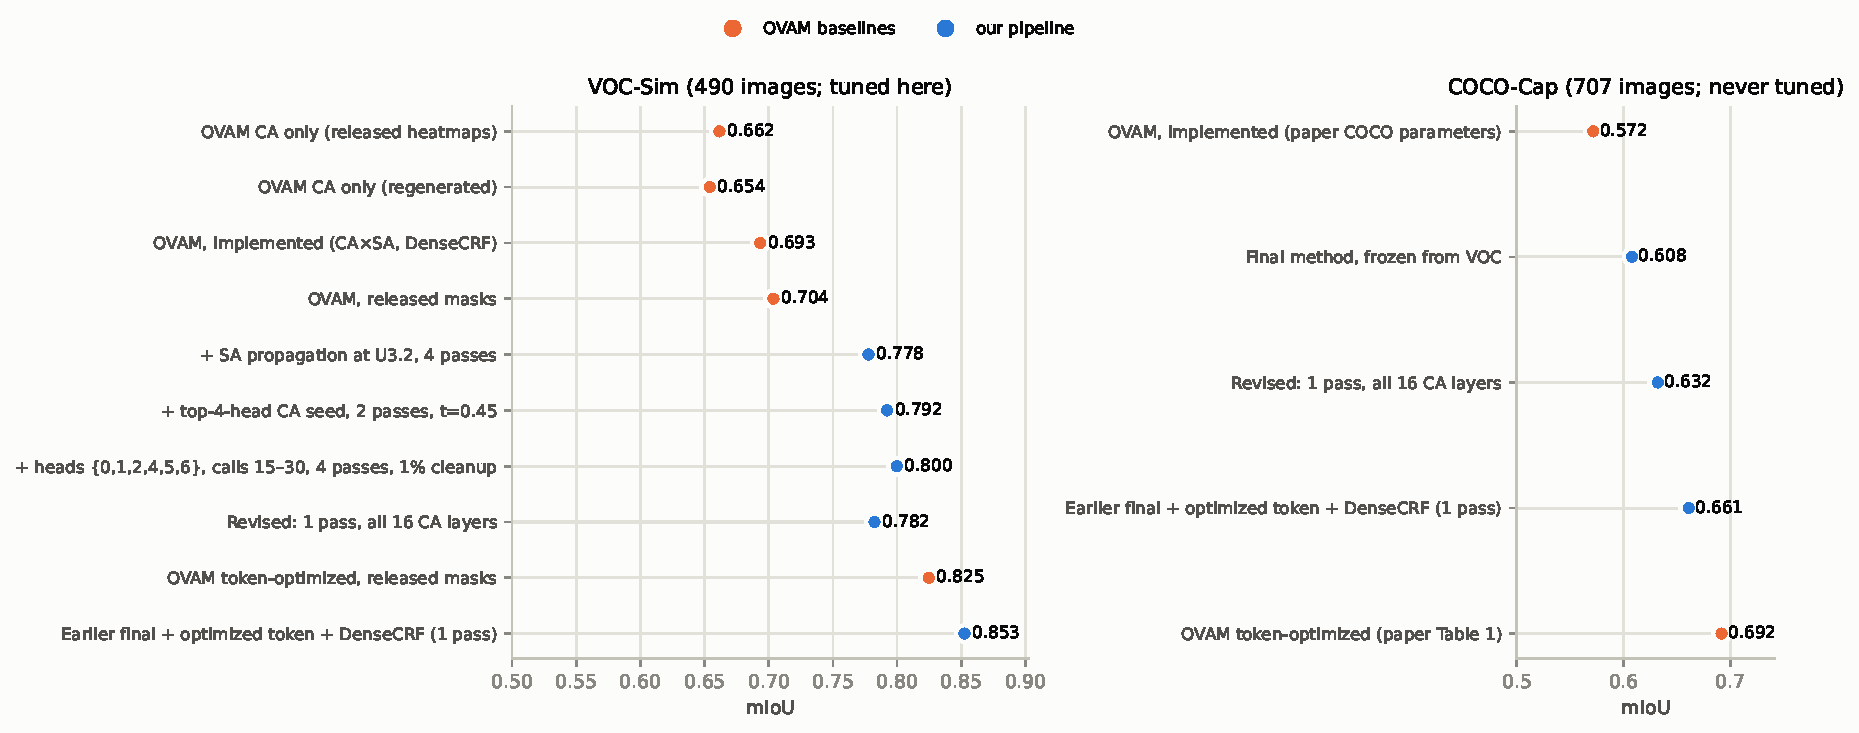
\includegraphics[width=0.8\linewidth]{evidence/figures/b_progression.pdf}
\caption{Each step of the earlier method and the baselines. VOC-Sim values are in-sample; COCO-Cap was never used to choose the earlier method.}\label{fig:rec_b_progression}
\end{figure}
\begin{figure}[H]\centering
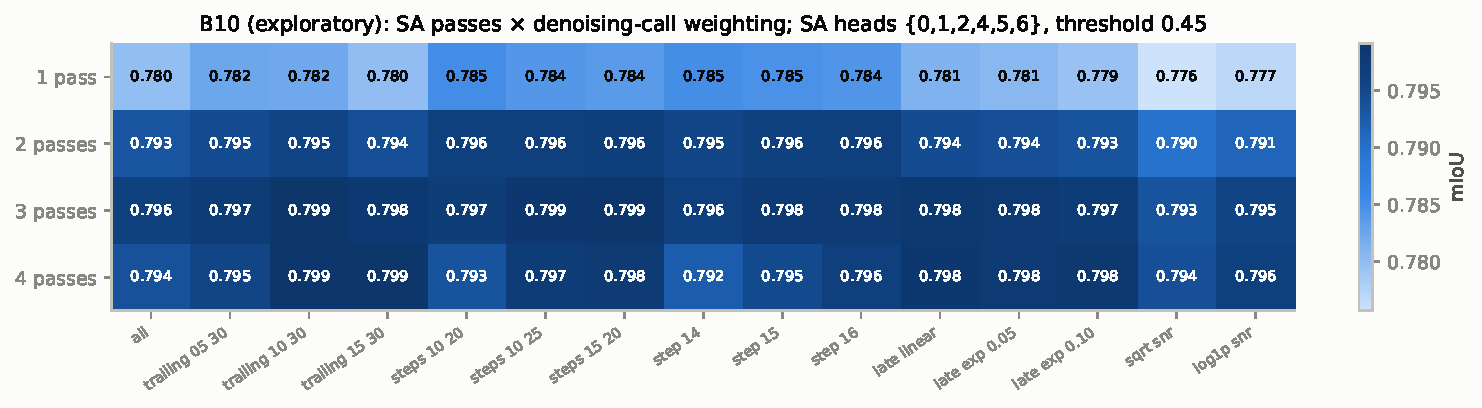
\includegraphics[width=0.8\linewidth]{evidence/figures/b_joint_passes_time.pdf}
\caption{Exploratory B10: SA passes by denoising-call weighting (in-sample).}\label{fig:rec_b_joint_passes_time}
\end{figure}
\begin{figure}[H]\centering
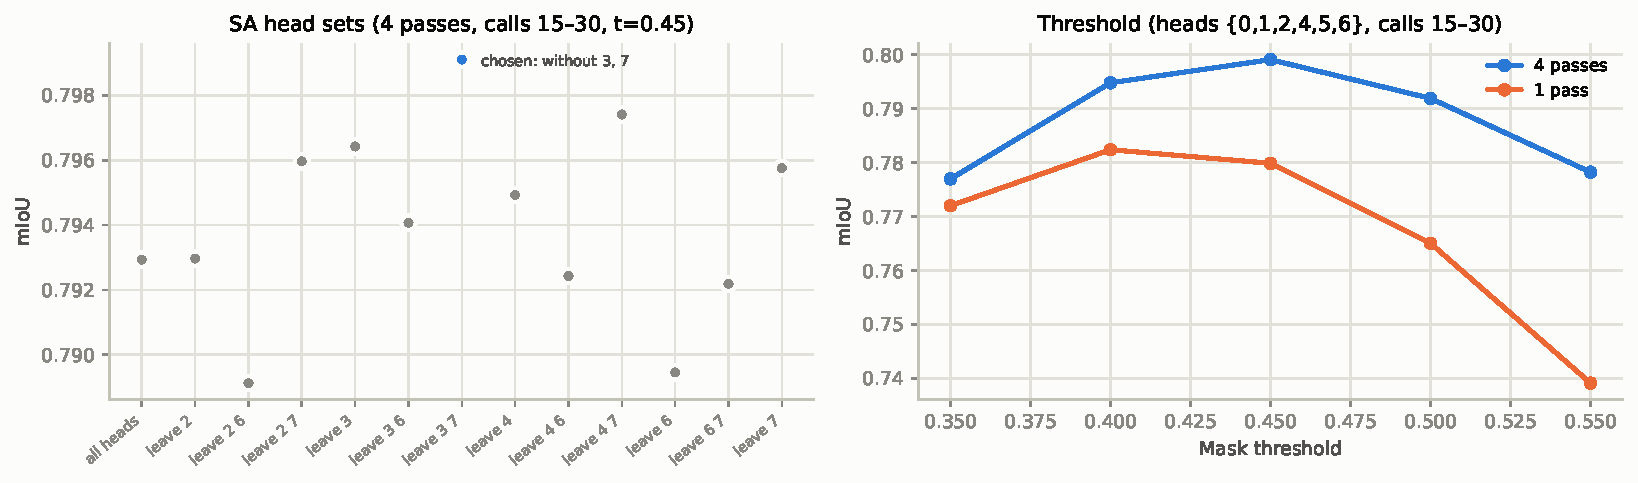
\includegraphics[width=0.8\linewidth]{evidence/figures/b_joint_heads_threshold.pdf}
\caption{Exploratory B10: SA head subsets and the mask threshold (in-sample).}\label{fig:rec_b_joint_heads_threshold}
\end{figure}
\begin{figure}[H]\centering
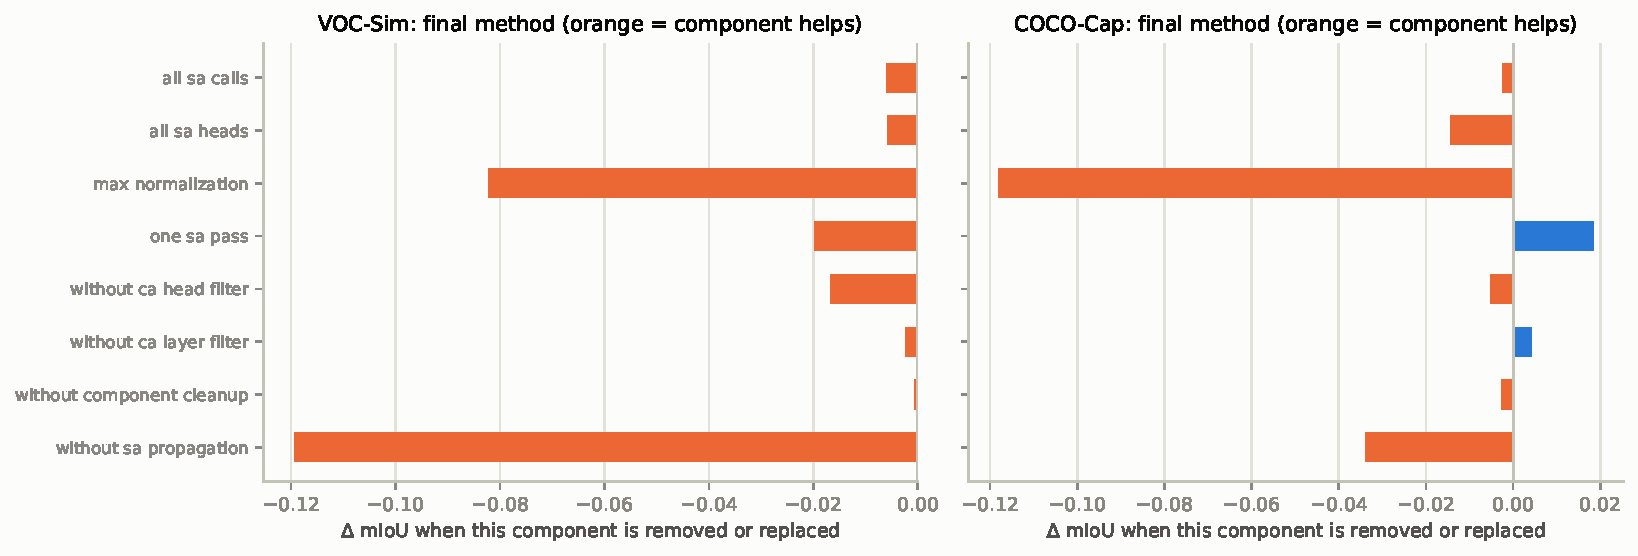
\includegraphics[width=0.8\linewidth]{evidence/figures/b_component_ablation.pdf}
\caption{Removing one component of the earlier method, on VOC-Sim and on the untuned COCO-Cap.}\label{fig:rec_b_component_ablation}
\end{figure}
\begin{figure}[H]\centering
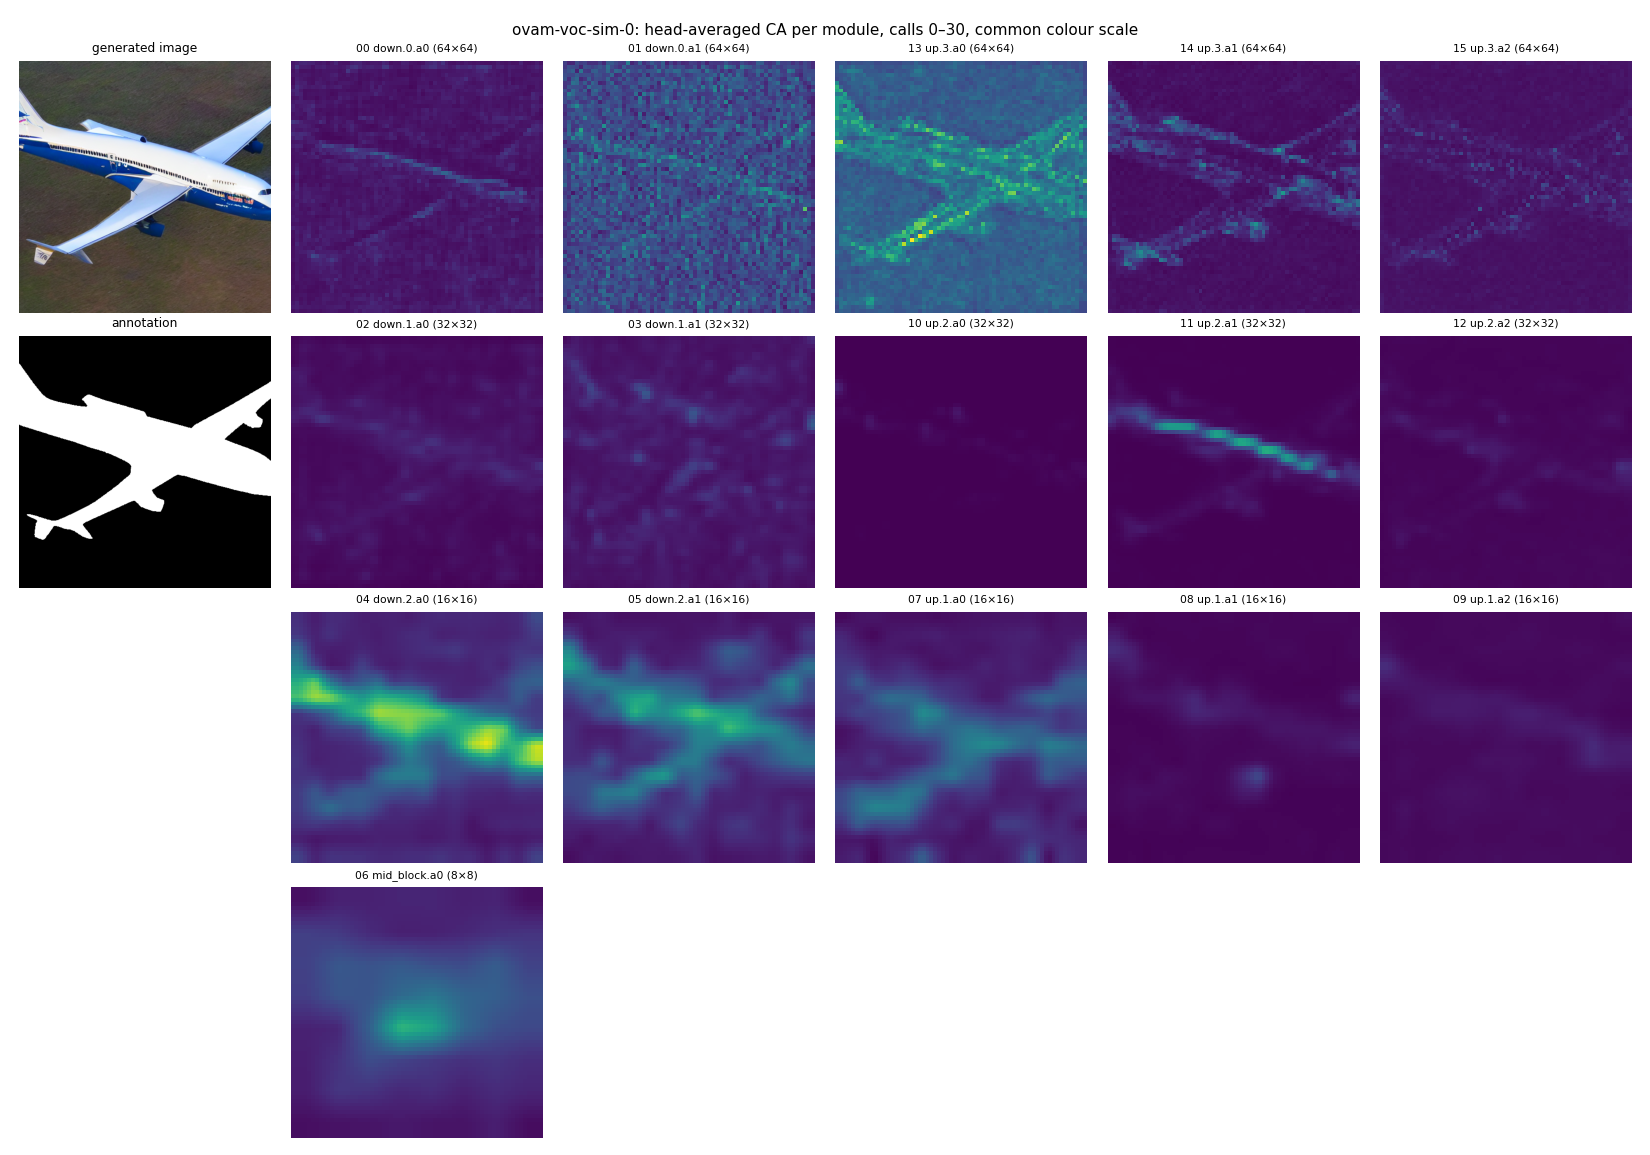
\includegraphics[width=0.7\linewidth]{evidence/figures/ovam-voc-sim-0_ca_modules.png}
\caption{Head-averaged cross-attention of every module for one VOC-Sim image (calls 0--30, common colour scale, one row per resolution). Further images in the evidence package.}\label{fig:rec_ca_modules}
\end{figure}


{
    \small
    \bibliographystyle{ieeenat_fullname}
    \bibliography{references}
}

\end{document}
